% Yue Li, July 2020

% This template is adapted from the previous template I wrote in 2017:
% University of Nottingham Thesis and Dissertation Template
% https://www.overleaf.com/latex/templates/university-of-nottingham-thesis-and-dissertation-template

% The current one includes more sample scripts in Chapter 4 Main Chapter, demonstrating the use of
% - Figures
% - Tables
% - Lists (for Research Questions and Hypotheses, etc.)
% - and PDF appendix in the Appendices chapter 

% This one is specifically shaped for a PhD thesis submission.
% Please double check with your faculty's thesis submission guideline.

% LENGTH AND PRESENTATION OF PhD THESIS
% The PhD thesis is normally about 80,000 words in length with an upper word-limit of 100,000 words. The Quality Manual states that ‘The thesis should not be more than 100,000 words in the case of PhD (inclusive of appendices, footnotes, tables, and bibliography); the University may withhold from examination a thesis that exceeds these word limits.'
% Your thesis/dissertation must be presented on A4 paper, single-sided, with 12 font typescript, with double spacing, and good quality printing to allow for reproduction. There should be a margin of at least 1.5 inches, preferably 2 inches (5cm), on the left side of the page, both for typescript and diagrams, to allow for binding. Other margins should be of at least 1 inch (2.5 cm).

\documentclass[a4paper,12pt,oneside]{report}
\usepackage[left=1.8in,right=1.2in,top=1in,bottom=1.2in]{geometry}

\setcounter{tocdepth}{2}

\usepackage{graphicx}
\usepackage{verbatim}
\usepackage{latexsym}
\usepackage[version=4]{mhchem}
\usepackage{mathchars}
\usepackage{setspace}
\usepackage[toc,page]{appendix}
\usepackage{float}
% \usepackage{subfigure}
\usepackage{subcaption}
\usepackage{url}
\usepackage{hyperref}
\hypersetup{
     colorlinks=true,
     linkcolor=black,
     filecolor=black,
     citecolor=black,
     urlcolor=blue,
}
% \usepackage[colorlinks=true]{hyperref}

%fonts; currently look weird with math.
%\usepackage[sfdefault]{roboto}
%\usepackage[T1]{fontenc}

%Per chapter appendix setup
\newcommand\appnums{% 
    \setcounter{figure}{0}
    \setcounter{table}{0}
    %\renewcommand\thefigure{\appendixname~\Alph{section}}}
    \renewcommand\thefigure{\thechapter.\Alph{figure}}
    \renewcommand\thetable{\thechapter.\Alph{table}}
    }
    
%reference setup
\usepackage[sectionbib, super, sort&compress, comma]{natbib}
\usepackage{chapterbib}
\setlength{\bibsep}{0.0pt}

\renewcommand{\bibname}{References}
\makeatletter 
\renewcommand\@biblabel[1]{#1.$\>\>$} 

%\usepackage{apalike}

% SI units, scientific notation
\usepackage{siunitx}
     
\usepackage{tabularx}
\usepackage{booktabs}
\usepackage{multirow}
\usepackage[normalem]{ulem}

% remove [demo] to actually display pdf. 
% Currently just displays empty pages
\usepackage[demo]{pdfpages}

\usepackage[htt]{hyphenat}

\usepackage[acronym]{glossaries}

% for H1. H2. enumeration
\usepackage{enumitem}

\usepackage{amsmath}
\usepackage{changepage}

\usepackage{acro}

% for C# code formatting
\usepackage{color}
\usepackage{listings}
\usepackage{spverbatim}
\lstloadlanguages{% Check Dokumentation for further languages ...
C,
C++,
csh,
Java
}

\definecolor{red}{rgb}{0.6,0,0} % for strings
\definecolor{blue}{rgb}{0,0,0.6}
\definecolor{green}{rgb}{0,0.8,0}
\definecolor{cyan}{rgb}{0.0,0.6,0.6}
\lstset{
basicstyle=\small\ttfamily, 
stringstyle=\color{black}\ttfamily, 
showstringspaces=false,
showspaces=false,
xleftmargin=17pt,
breaklines=true,
}
\usepackage{caption}

% number subsubsections
\setcounter{secnumdepth}{3}

% for table of contents to show Chapter
\usepackage{tocloft,calc}
\renewcommand{\cftchappresnum}{Chapter }
\AtBeginDocument{\addtolength\cftchapnumwidth{\widthof{Chapter}}}

% for table of contents to show Appendix
\renewcommand{\cftchappresnum}{\chaptername\space}
\setlength{\cftchapnumwidth}{\widthof{Appendix}}
\makeatletter
\g@addto@macro\appendix{%
  \addtocontents{toc}{%
    \protect\renewcommand{\protect\cftchappresnum}{\appendixname\space}
  }%
}

% mini table of content
\usepackage{minitoc}
\setlength{\mtcindent}{24pt}
\renewcommand{\mtcoffset}{0pt}
\mtcsetoffset{minitoc}{0pt} \setlength{\mtcskipamount}{\bigskipamount}
\mtcsetdepth{minitoc}{2} \mtcsetfont{minitoc}{*}{\small\rmfamily\upshape\mdseries} \mtcsetfont{minitoc}{section}{\small\rmfamily\upshape\bfseries}
\setcounter{mtc}{9}

\usepackage{fancyhdr}
% \fancypagestyle{plain}{%  the preset of fancyhdr 
%     \fancyhf{} % clear all header and footer fields
%     \fancyhead[C]{\textbf{\rightmark}}
%     % \fancyhead[R]{\textbf{\rightmark}}
%     % \pagenumbering{arabic}
%     % \fancyfoot[R]{\thepage}
%     \renewcommand{\headrulewidth}{0pt}
%     \renewcommand{\footrulewidth}{0pt}}
    
\fancypagestyle{front}{% style for TOC, LOF, LOT
  \fancyhf{}
  \renewcommand{\headrulewidth}{0pt}
  \cfoot{\thepage}
}
\fancypagestyle{main}{% style for the mainmatter
  \fancyhf{}
  \fancyhead[C]{\slshape \rightmark}
  \fancyfoot[C]{\thepage}
  \renewcommand\headrulewidth{.4pt}
}
\makeatletter
  \newcommand\frontpagestyle{\cleardoublepage\pagestyle{front}\let\ps@plain\ps@front}
  \newcommand\mainpagestyle{\cleardoublepage\pagestyle{main}\let\ps@plain\ps@main}
\makeatother

\setlength{\parskip}{\medskipamount}  % a little space before a \par
\setlength{\parindent}{0pt}	      % don't indent first lines of paragraphs
% %UHEAD.STY  If this is included after \documentstyle{report}, it adds
% an underlined heading style to the LaTeX report style.
% \pagestyle{uheadings} will put underlined headings at the top
% of each page. The right page headings are the Chapter titles and
% the left page titles are supplied by \def\lefthead{text}.

% Ted Shapin, Dec. 17, 1986

\makeatletter
\def\chapapp2{Chapter}

\def\appendix{\par
 \setcounter{chapter}{0}
 \setcounter{section}{0}
 \def\chapapp2{Appendix}
 \def\@chapapp{Appendix}
 \def\thechapter{\Alph{chapter}}}

\def\ps@uheadings{\let\@mkboth\markboth
% modifications
\def\@oddhead{\protect\underline{\protect\makebox[\textwidth][l]
		{\sl\rightmark\hfill\rm\thepage}}}
\def\@oddfoot{}
\def\@evenfoot{}
\def\@evenhead{\protect\underline{\protect\makebox[\textwidth][l]
		{\rm\thepage\hfill\sl\leftmark}}}
% end of modifications
\def\chaptermark##1{\markboth {\ifnum \c@secnumdepth >\m@ne
 \chapapp2\ \thechapter. \ \fi ##1}{}}%
\def\sectionmark##1{\markright {\ifnum \c@secnumdepth >\z@
   \thesection. \ \fi ##1}}}
\makeatother
%%From: marcel@cs.caltech.edu (Marcel van der Goot)
%%Newsgroups: comp.text.tex
%%Subject: illegal modification of boxit.sty
%%Date: 28 Feb 92 01:10:02 GMT
%%Organization: California Institute of Technology (CS dept)
%%Nntp-Posting-Host: andromeda.cs.caltech.edu
%%
%%
%%Quite some time ago I posted a file boxit.sty; maybe it made it
%%to some archives, although I don't recall submitting it. It defines
%%	\begin{boxit}
%%	...
%%	\end{boxit}
%%to draw a box around `...', where the `...' can contain other
%%environments (e.g., a verbatim environment). Unfortunately, it had
%%a problem: it did not work if you used it in paragraph mode, i.e., it
%%only worked if there was an empty line in front of \begin{boxit}.
%%Luckily, that is easily corrected.
%%
%%HOWEVER, apparently someone noticed the problem, tried to correct it,
%%and then distributed this modified version. That would be fine with me,
%%except that:
%%1. There was no note in the file about this modification, it only has my
%%   name in it.
%%2. The modification is wrong: now it only works if there is *no* empty
%%   line in front of \begin{boxit}. In my opinion this bug is worse than
%%   the original one.
%%
%%In particular, the author of this modification tried to force an empty
%%line by inserting a `\\' in the definition of \Beginboxit. If you have
%%a version of boxit.sty with a `\\', please delete it. If you have my
%%old version of boxit.sty, please also delete it. Below is an improved
%%version.
%%
%%Thanks to Joe Armstrong for drawing my attention to the bug and to the
%%illegal version.
%%
%%                                          Marcel van der Goot
%% .---------------------------------------------------------------
%% | Blauw de viooltjes,                    marcel@cs.caltech.edu
%% |    Rood zijn de rozen;
%% | Een rijm kan gezet
%% |    Met plaksel en dozen.
%% |


% boxit.sty
% version: 27 Feb 1992
%
% Defines a boxit environment, which draws lines around its contents.
% Usage:
%   \begin{boxit}
%	... (text you want to be boxed, can contain other environments)
%   \end{boxit}
%
% The width of the box is the width of the contents.
% The boxit* environment behaves the same, except that the box will be
% at least as wide as a normal paragraph.
%
% The reason for writing it this way (rather than with the \boxit#1 macro
% from the TeXbook), is that now you can box verbatim text, as in
%   \begin{boxit}
%   \begin{verbatim}
%   this better come out in boxed verbatim mode ...
%   \end{verbatim}
%   \end{boxit}
%
%						Marcel van der Goot
%						marcel@cs.caltech.edu
%

\def\Beginboxit
   {\par
    \vbox\bgroup
	   \hrule
	   \hbox\bgroup
		  \vrule \kern1.2pt %
		  \vbox\bgroup\kern1.2pt
   }

\def\Endboxit{%
			      \kern1.2pt
		       \egroup
		  \kern1.2pt\vrule
		\egroup
	   \hrule
	 \egroup
   }	

\newenvironment{boxit}{\Beginboxit}{\Endboxit}
\newenvironment{boxit*}{\Beginboxit\hbox to\hsize{}}{\Endboxit}
% Created by Yue Li, June 2017

\pagestyle{empty}

\setlength{\parskip}{0em}
\setlength{\parindent}{0em}

\makeatletter  %to avoid error messages generated by "\@". Makes Latex treat "@" like a letter

\linespread{1.5}
\def\submitdate#1{\gdef\@submitdate{#1}}
\def\degree#1{\gdef\@degree{#1}}
\def\studentid#1{\gdef\@studentid{#1}}
\def\supervisor#1{\gdef\@supervisor{#1}}

\def\maketitle{
    
  \begin{titlepage}{
    
    \centering{
    
\includegraphics[width=0.5\columnwidth]{images/nottingham-logo.png}} \par
    % \textbf{International Doctoral Innovation Centre}
    
    \vskip 1in \par 
    \LARGE {\bf \@title}
    
    \vskip 0.5in \par
    \normalsize {Thesis submitted to the University of Nottingham for the degree of \\\bf{\@degree}, \@submitdate.}

  }
  \vskip 0.3in \par
  \large {\bf \@author} \par
  \large {\bf \@studentid}
  
  \vskip 0.3in \par
  \normalsize {Supervised by} \par
  \normalsize {\textbf{\@supervisor}}
  \vskip 0.3in \par
%   \normalsize { School of Computer Science \par
%   University of Nottingham}

  \vskip 0.5in \par
%   \normalsize {I hereby declare that this dissertation is all my own work, except as indicated in the text: }

  \vskip 0.5in 
  \normalsize {Signature \underline{\hspace{1.5in}}}
  
  \vskip 0.1in
  \normalsize {Date \underline{\hspace{0.5in}} / \underline{\hspace{0.5in}} / \underline{\hspace{0.5in}}}
  
  %%%%%%%%%%
  %*Only include this sentence below if you do have all necessary rights and consents. For example, if you have including photographs or images from the web or from other papers or documents then you need to obtain explicit consent from the original copyright owner. If in doubt, delete this sentence. See Copyright Information: http://eprints.nottingham.ac.uk/copyrightinfo.html for more details.
  %%%%%%%%%%
  
%   \vskip 0.4in \par
%   \normalsize {I hereby declare that I have all necessary rights and consents to publicly distribute this dissertation via the University of Nottingham's e-dissertation archive.}

  %%%%%%%%%%
  %Only include this sentence below if there is some reason why your dissertation should not be accessible for some period of time, for example if it contains information which is commercially sensitive or might compromise an Intellectual Property claim. If included, fill in the date from which access should be allowed.
  %%%%%%%%%%

%   \vskip 0.4in \par
%   \normalsize {Public access to this dissertation is restricted until: DD/MM/YYYY}
  
  \end{titlepage}
}

\def\titlepage{
  \newpage
  \centering
  \linespread{1}
  \normalsize
  \vbox to \vsize\bgroup\vbox to 9in\bgroup
}
\def\endtitlepage{
  \par
  \kern 0pt
  \egroup
  \vss
  \egroup
  \cleardoublepage
}

\def\abstract{
  \begin{center}{
    \large\bf Abstract}
  \end{center}
  \small
  %\def\baselinestretch{1.5}
  \linespread{1.5}
  \normalsize
}
\def\endabstract{
  \par
}

\newenvironment{acknowledgements}{
  \cleardoublepage
  \begin{center}{
    \large \bf Acknowledgements}
  \end{center}
  \small
  \linespread{1.5}
  \normalsize
}{\cleardoublepage}
\def\endacknowledgements{
  \par
}

\def\preface{
    \pagenumbering{roman}
    \pagestyle{plain}
    \doublespacing
}

\setlength\cftbeforechapskip{1pt}

\def\body{
	\setcounter{tocdepth}{2}
	\setcounter{minitocdepth}{2}
	
	\dominitoc 
	\dominilof 
	\dominilot
	
    \tableofcontents
    \pagestyle{plain}
    
    \cleardoublepage
    \listoftables
    \addstarredchapter{List of Tables}
    \chaptermark{List of Tables}
    \pagestyle{plain}
    
    \cleardoublepage
    \addstarredchapter{List of Figures}
    \chaptermark{List of Figures}
    \listoffigures
    \pagestyle{plain}
    
    \cleardoublepage
    \printnoidxglossary[type=\acronymtype,style=index,nonumberlist,title=Abbreviations, nogroupskip=true]
    \printnoidxglossary[title=Nomenclature]
    \addstarredchapter{Abbreviations}
    \chaptermark{Abbreviations}
    \pagestyle{plain}
    
    \cleardoublepage
    \pagenumbering{arabic}
    \doublespacing
    
    \adjustmtc
}

\makeatother  %to avoid error messages generated by "\@". Makes Latex treat "@" like a letter

\newcommand{\ipc}{{\sf ipc}}
\newcommand{\Prob}{\bbbp}
\newcommand{\Real}{\bbbr}
\newcommand{\real}{\Real}
\newcommand{\Int}{\bbbz}
\newcommand{\Nat}{\bbbn}

\newcommand{\NN}{{\sf I\kern-0.14emN}}   % Natural numbers
\newcommand{\ZZ}{{\sf Z\kern-0.45emZ}}   % Integers
\newcommand{\QQQ}{{\sf C\kern-0.48emQ}}   % Rational numbers
\newcommand{\RR}{{\sf I\kern-0.14emR}}   % Real numbers
\newcommand{\KK}{{\cal K}}
\newcommand{\OO}{{\cal O}}
\newcommand{\AAA}{{\bf A}}
\newcommand{\HH}{{\bf H}}
\newcommand{\II}{{\bf I}}
\newcommand{\LL}{{\bf L}}
\newcommand{\PP}{{\bf P}}
\newcommand{\PPprime}{{\bf P'}}
\newcommand{\QQ}{{\bf Q}}
\newcommand{\UU}{{\bf U}}
\newcommand{\UUprime}{{\bf U'}}
\newcommand{\zzero}{{\bf 0}}
\newcommand{\ppi}{\mbox{\boldmath $\pi$}}
\newcommand{\aalph}{\mbox{\boldmath $\alpha$}}
\newcommand{\bb}{{\bf b}}
\newcommand{\ee}{{\bf e}}
\newcommand{\mmu}{\mbox{\boldmath $\mu$}}
\newcommand{\vv}{{\bf v}}
\newcommand{\xx}{{\bf x}}
\newcommand{\yy}{{\bf y}}
\newcommand{\zz}{{\bf z}}
\newcommand{\oomeg}{\mbox{\boldmath $\omega$}}
\newcommand{\res}{{\bf res}}
\newcommand{\cchi}{{\mbox{\raisebox{.4ex}{$\chi$}}}}
%\newcommand{\cchi}{{\cal X}}
%\newcommand{\cchi}{\mbox{\Large $\chi$}}

% Logical operators and symbols
\newcommand{\imply}{\Rightarrow}
\newcommand{\bimply}{\Leftrightarrow}
\newcommand{\union}{\cup}
\newcommand{\intersect}{\cap}
\newcommand{\boolor}{\vee}
\newcommand{\booland}{\wedge}
\newcommand{\boolimply}{\imply}
\newcommand{\boolbimply}{\bimply}
\newcommand{\boolnot}{\neg}
\newcommand{\boolsat}{\!\models}
\newcommand{\boolnsat}{\!\not\models}


\newcommand{\op}[1]{\mathrm{#1}}
\newcommand{\s}[1]{\ensuremath{\mathcal #1}}

% Properly styled differentiation and integration operators
\newcommand{\diff}[1]{\mathrm{\frac{d}{d\mathit{#1}}}}
\newcommand{\diffII}[1]{\mathrm{\frac{d^2}{d\mathit{#1}^2}}}
\newcommand{\intg}[4]{\int_{#3}^{#4} #1 \, \mathrm{d}#2}
\newcommand{\intgd}[4]{\int\!\!\!\!\int_{#4} #1 \, \mathrm{d}#2 \, \mathrm{d}#3}

% Large () brackets on different lines of an eqnarray environment
\newcommand{\Leftbrace}[1]{\left(\raisebox{0mm}[#1][#1]{}\right.}
\newcommand{\Rightbrace}[1]{\left.\raisebox{0mm}[#1][#1]{}\right)}

% Funky symobols for footnotes
\newcommand{\symbolfootnote}{\renewcommand{\thefootnote}{\fnsymbol{footnote}}}
% now add \symbolfootnote to the beginning of the document...

\newcommand{\normallinespacing}{\renewcommand{\baselinestretch}{1.5} \normalsize}
\newcommand{\mediumlinespacing}{\renewcommand{\baselinestretch}{1.2} \normalsize}
\newcommand{\narrowlinespacing}{\renewcommand{\baselinestretch}{1.0} \normalsize}
\newcommand{\bump}{\noalign{\vspace*{\doublerulesep}}}
\newcommand{\cell}{\multicolumn{1}{}{}}
\newcommand{\spann}{\mbox{span}}
\newcommand{\diagg}{\mbox{diag}}
\newcommand{\modd}{\mbox{mod}}
\newcommand{\minn}{\mbox{min}}
\newcommand{\andd}{\mbox{and}}
\newcommand{\forr}{\mbox{for}}
\newcommand{\EE}{\mbox{E}}

\newcommand{\deff}{\stackrel{\mathrm{def}}{=}}
\newcommand{\syncc}{~\stackrel{\textstyle \rhd\kern-0.57em\lhd}{\scriptstyle L}~}

\def\coop{\mbox{\large $\rhd\!\!\!\lhd$}}
\newcommand{\sync}[1]{\raisebox{-1.0ex}{$\;\stackrel{\coop}{\scriptscriptstyle
#1}\,$}}

\newtheorem{definition}{Definition}[chapter]
\newtheorem{theorem}{Theorem}[chapter]

\newcommand{\Figref}[1]{Figure~\ref{#1}}
\newcommand{\fig}[3]{
 \begin{figure}[!ht]
 \begin{center}
 \scalebox{#3}{\includegraphics{figs/#1.ps}}
 \vspace{-0.1in}
 \caption[ ]{\label{#1} #2}
 \end{center}
 \end{figure}
}

\newcommand{\figtwo}[8]{
 \begin{figure}
 \parbox[b]{#4 \textwidth}{
 \begin{center}
 \scalebox{#3}{\includegraphics{figs/#1.ps}}
 \vspace{-0.1in}
 \caption{\label{#1}#2}
 \end{center}
 }
 \hfill
 \parbox[b]{#8 \textwidth}{
 \begin{center}
 \scalebox{#7}{\includegraphics{figs/#5.ps}}
 \vspace{-0.1in}
 \caption{\label{#5}#6}
 \end{center}
 }
 \end{figure}
}

%for changing offsets when pdfs inserted
\newlength{\originalVOffset}
\newlength{\originalHOffset}
\setlength{\parskip}{1em}


% define all abbreviations used in the thesis
\newacronym{vr}{VR}{Virtual Reality}
\newacronym{ar}{AR}{Augmented Reality}
\newacronym{hvar}{HVAR}{Hybrid Virtual and Augmented Reality}

\makenoidxglossaries

% define research questions so that the phrasing of words are consistent.
\newcommand{\rqone}{First research question?}
\newcommand{\rqtwo}{Second research question?}
\newcommand{\rqthree}{Third research question?}
    
\begin{document}
\symbolfootnote
%\DeclareBackupCountersGroupName{pagebackup}
%\AssignBackupCounters[name=pagebackup]{page}

\newcounter{opagenum}
\setcounter{opagenum}{\thepage}

\title{Turbostratic carbons from \ce{CO2} capture: Novel synthetic methods, and development of improved experimental and computational techniques for understanding the relationship between porosity \ce{CO2} capacity}

\makeatletter
\let\inserttitle\@title
\makeatother

\author{L. Scott Blankenship}
\submitdate{July 2022}
\degree{Doctor of Philosophy}
\studentid{4343286}
\supervisor{\\Professor Robert Mokaya\\Dr Begum Tokay}

\normallinespacing
\maketitle

\preface

\cleardoublepage

\chapter*{Abstract} \label{Abstract}
\addcontentsline{toc}{chapter}{Abstract}

As of 2021, the atmospheric concentration of \ce{CO2} is 412 ppm and continues to rise. It is well established that these concentrations are resulting in rising temperatures, an increased incidence of extreme weather, and thus unspeakably disastrous consequences for all life. It follows then that \ce{CO2} capture and removal technologies must be rapidly developed to ensure the longevity of human society. One area of research is \ce{CO2} capture \textit{via} \gls{physisorption} onto porous materials and in particular on the easily synthesised \glspl{turbostratic carbon}. This application requires fine control over porosity (surface area, pore volume, pore size) according to conditions of sorption, and it therefore follows that both the ability to precisely measure pore sizes, as well as a definitive knowledge of the relationship between \ce{CO2} uptake capacity and pore size is needed. This thesis attempts to address all three of these issues.

In terms of routes to \glspl{activated carbon}, this work investigates two principal synthetic methods. Firstly in chapter \ref{ch:cbs} - developing on the author's previous work - a simplification of the production of \glspl{turbostratic carbon} from unwrapped \acrfullpl{ucf} was attempted by \gls{activation} of whole \acrfullpl{ucb} with \ce{KOH}. The simplified method resulted in much less porosity as compared to the previous work (maximal $A_{BET}$ of 4300 compared with 1960 $\rm m^2\ g^{-1}$) and the samples derived by this method possess a hierarchical - as opposed to narrow, microporous - \acrfull{psd}. Nevertheless, these new materials may perform well for \ce{CO2} capture in \acrfull{psa} applications. \Gls{pyrolysis} of \acrshortpl{ucb} in the absence of a \gls{porogen} created minimal porosity, perhaps as a result of contaminants present from the \acrshort{ucb} wrapping paper. 

The other approach to activation used (chapter \ref{ch:impregnation}) is a set of methods which have been collectively coined as impregnation routes, i.e. methods which attempt to achieve close contact between precursor and the activating species whilst maintaining a homogeneous distribution of the latter throughout the former. Impregnation was achieved through (i) the hydrothermal carbonisation of \acrfull{sd} with \ce{KOH} prior to pyrolysis, as well as (ii) direct activation of a polymeric sodium salt, \acrfull{nc}. In both cases, \acrshortpl{psd} achieved were generally narrow and situated principally in the small \gls{micropore} region, making the products potential candidates for low pressure \ce{CO2} capture. Both sets of materials also showed unexpected features, \acrshort{sd}-derived samples having extremely low bulk density, and those obtained from \acrshort{nc} exhibiting reduction in porosity at surprisingly low \gls{porogen}:precursor ratios. The latter of these suggests pore formation effects outside of the caustic nature of \gls{porogenesis} with \ce{Na} compounds, and is a potential route for further investigation of \gls{activation} mechanisms.

For materials derived through the synthetic routes mentioned above, reliable, accurate, and efficient isothermal porosimetry proved difficult due to poor diffusion of \ce{N2} into the materials' pores. As such, alternative porosimetric techniques were investigated in chapter \ref{ch:dual_isotherm}. It was found that dual isotherm porosimetry using \ce{O2} and \ce{H2} isotherms measured at -196 $\rm ^{\circ}C$ results not only in more expedient equilibration of the sorptive-sorbent system, but allows the measurement of sub-angstrom level developments in porosity associated with changes in quantity of \gls{porogen} used. These subtle developments in porosity are not measurable through traditional porosimetry using \ce{N2}. 

As for improving the understanding of the relationship between \ce{CO2} uptake as a function of pressure and pore size, chapter \ref{ch:pyPUC} details the development and deployment of the \acrfull{pypuc} which, using experimental \acrshortpl{psd} and gravimetric gas uptake isotherms applies a brute force approach to determine the correlation between porosity within some pore width range and \ce{CO2} uptake at a given pressure. This is performed for all user-defined pore width ranges and pressures, and correlation coefficients are compared to give optimum pore size ranges, $\Omega$ at each pressure. When applied to \ce{CO2} uptake on \glspl{turbostratic carbon}, it was confirmed that $\Omega$ broadens with increasing pressure. In addition, the relationship between $\Omega$ and pressure-dependent \ce{CO2} uptake was calculated to a more granular level of detail than has been previously reported. Furthermore, following on from findings in chapter \ref{ch:dual_isotherm} it was found that these relationships at low pressures are best described using dual isotherm \ce{O2}/\ce{H2} porosimetry.
\addstarredchapter{Statutory Declaration}
\chaptermark{Statutory Declaration}

\chapter*{Statutory Declaration}
\cleardoublepage

\chapter*{Acknowledgements}
\addcontentsline{toc}{chapter}{Acknowledgements}

It has been a long and unusual journey to finally come to submitting my thesis. As with anything such as this, it would not have been possible without the help of a hoard of disparate delightful humans. The first I'd like to acknowledge of course is my supervisor, Robert Mokaya. From the beginning (prior to my master's research) you have accepted and encouraged every half-planned route of investigation I've decided to go down. I look forward to continuing to work with you. I'm also grateful to all current and former members of the Mokaya group, but in particular Alison Taylor who trained me on many synthetic and analytical techniques as well as Thria Alkhaldi with whom it is always fun to discuss ideas for experiments. I'd like to thank the technical staff in the School of Chemistry, in particular Mark Guyler and Neil Barnes for their essentially help and calm heads when things (frequently!) break, or indeed when I break them even worse than they were originally broken. Neil also provided a vital listening ear when I was extremely stressed and frustrated in my second year. On that topic, thanks to everyone who frequents the school smoking area for allowing me to vent when needed.

Outside of the University of Nottingham, I'd like to thank Jacek Jagiello for taking an avid interest in my work and the many chats we had about adsorption theory. In a similar vein, discussions with Paul Iacomi have always been so insightful. He alongside Hassan Akhtar have been a great help in improving my infantile computer code at times. More recently, abstract mathematical discussions with my dear \textgreek{Ηρώ} have been great fun and helped me look at my work in a different way. Two broad groups of friends that may not have donated technical knowledge but lent more emotional support are those at Kunsthaus and its extended universe, and the Whitchurch OGs - you know who you are. From the latter group I'd like to single out my best mate Jonnie Felton, and from the former Raffa and Mattia who have patiently listened to me babble about some incoherent abstract concept for which I have not armed them adequately with the prerequisite knowledge.

I suppose that just leaves my family. My younger sisters have all served as cheerleaders in their own right and I'm thankful for all three of you. Aunt Mimi and Grandma Joy you've always told me I can be anything I want to be and that has inspired (an at times dangerous) amount of self-confidence which has pushed me through this PhD. But the biggest thanks goes to my mother Cheryl. Apart from preventing me from dying at various points before I was five and being a great Mom in general you literally taught me how to read and write, so none of this would be possible without you. You inspired and encouraged a lifelong love of learning in me and that is truly something that money cannot buy. 
\cleardoublepage
\addcontentsline{toc}{chapter}{List of Publications}

\chapter*{List of Publications}

This thesis resulted in the following publications;

\begin{enumerate}[label=\Roman*]
    \item \underline{L. Scott Blankenship} and Robert Mokaya, \textbf{Modulating the porosity of carbons for improved adsorption of hydrogen, carbon dioxide, and methane: a review}, \textit{Materials Advances}, 2022 (3), 1905-1930
    \item \underline{L. Scott Blankenship}, Jacek Jagiello and Robert Mokaya, \textbf{Confirmation of pore formation mechanisms in biochars and activated carbons by dual isotherm analysis}, \textit{Materials Advances}, 2022
    \item \underline{L. Scott Blankenship}, Nawaf Albeladi, Thria Alkhaldi, Asma Madkhali and Robert Mokaya, \textbf{Brute force determination of optimum pore sizes for \ce{CO2} uptake}, \textit{Journal}, 2022
    
\end{enumerate}

\paragraph{The author's contribution to these publications;}
In all cases, the author wrote the manuscript. For Publication I the author performed the literature review. In the case of Publication II the author did all experimental work and conceptualised the project and performed the majority of data analysis. For Publication III the author contributed to experimental work, conceptualised and designed the software needed to perform the analyses, and performed all data analysis.

\newpage
In addition to this thesis, the author has contributed to this publication;

\begin{enumerate}[resume, label=\Roman*]
    \item Ryan R Larder, Thomas M Bennett, \underline{L. Scott Blankenship}, Jesum A Fernandes, Bethany K Husband, Rachel L Atkinson, Matthew J Derry, Daniel TW Toolan, Higor A Centurion, Paul D Topham, Renato V Gonçalves, Vincenzo Taresco, Steven M Howdle, \textbf{Porous hollow \ce{TiO2} microparticles for photocatalysis: exploiting novel ABC triblock terpolymer templates synthesised in supercritical \ce{CO2}}, \textit{Polymer Chemistry}, 2021 (12), 19, 2904-2913
    
\end{enumerate}

The following publications were produced from the author's MSc, and form the basis of work in chapter \ref{ch:cbs}.

\begin{enumerate}[resume, label=\Roman*]
    \item \underline{L. Scott Blankenship}, Norah Balahmar and Robert Mokaya, \textbf{Oxygen-rich microporous carbons with exceptional hydrogen storage capacity}, \textit{Nature Communications}, 2017 (8), 1–12
    \item \underline{L. Scott Blankenship} and Robert Mokaya, \textbf{Cigarette butt-derived carbons have ultra-high surface area and unprecedented hydrogen storage capacity}, \textit{Energy \& Environmental Science}, 2017 (10), 2552–2562
    
\end{enumerate}

\newpage
\tableofcontents

\frontpagestyle

%\body

\mainpagestyle

% not working yet
%\setcounter{savepage}{\value{page}}
\pagenumbering{arabic}

\chapter{Introduction}
\label{ch:introduction}
The following sections provide the essential background of the concepts and applications of the experimental and computational work contained within this thesis. While it is indeed sufficiently thorough, the author provides for convenience, his published review on the modulation of the porosity of carbons for uptake of various gases (\ref{pub:review}) as appendix \ref{ap:review}. This provides much broader information of the synthesis of porous carbons outside of just the \glspl{turbostratic carbon} which are examined in this work, and the measurement of porosity, as well as the relationship between porosity and uptake of different sorbents. 

\newpage

\section{Synthesis of turbostratic carbons}

\Glspl{turbostratic carbon} are semi-ordered carbonaceous materials characterised as having high surface area due to an extensively porous structure. Gases such as \ce{CO2} can be physisorbed onto the surface of the material making for facile regeneration.\citep{Kuramochi2012Comparative, Ghosh2016} These characteristics make the material attractive for \ce{CO2} capture. In addition, these materials are chemically and thermally robust, meaning that they are suitable for industrial applications.\citep{Kuramochi2012Comparative, Coromina2016, HaffnerStaton2016High} As the only requirement for a porous carbon precursor  is  that  it have a high carbon content,  these materials can be  synthesized  from a  range  of cheap, and even renewable or waste-derived precursors.\citep{Sevilla2014Energy, Sun2017, Titirici2010Chemistry, Blankenship2017Cigarette, Ariharan2018}

The porosity of a carbonaceous material is typically developed \textit{via} a pyrolysis process wherein a graphitic structure is established. Pores are then further constructed \textit{via} intercalation of species inbetween the graphitic layers, either by gases,\citep{Gonzalez2009} or metal ions such as Na or K.\citep{Sevilla2014Energy, Osswald2009Porosity, Wang2012KOH, RuizFernandez2011} Both of these intercalating agents can come from the raw material itself or be added to improve pore development. Further pore development comes as the result of chemical reactions, such as the oxidation of carbon to form carbonates or dehydration reactions which form cross-links between graphitic layers.\citep{Sevilla2014Energy, Wang2012KOH, Prahas2008} These processes yield pores of a slit-like geometry, whose width is defined by the distance between two adjacent carbon walls, while the other dimensions are not usually defined (or assumed to be infinite).\citep{Sevilla2019, Everett1976Adsorption}

In order to facilitate high levels of porosity development, polymeric carbohydrates and sugars are often hydrothermally carbonised prior to activation with oxidative chemical \glspl{porogen} such as \ce{KOH}, by heating in water under high pressure to form \gls{hydrochar}. This results in a low-surface area material (\qty{\sim30}{\metre\squared\per\gram}) composed of microspheres with hydrophilic reactive oxygen moieties at  the  surface, while also increasing the overall oxygen concentration of the material.\citep{Titirici2010Chemistry, Sevilla2011High} Dried \gls{hydrochar} is then more susceptible to \ce{KOH}-activation due to the improved reactivity between K and the oxygen-rich material.\citep{Sevilla2011High, Sevilla2009Chemical} Indeed, some carbohydrates will not activate unless they have been first hydrothermally carbonised.\citep{Ares2014}

\subsection{From Cigarette Butts}

\acrfullpl{ucb} pose a large environmental hazard as a result of (i) being made of non-biodegradable \acrfull{ca} as well as (ii) containing a myriad of toxic chemicals.\citep{Slaughter2011, Puls2011, chevalier2018nano} As they are the most common waste material worldwide, there have been attempts to reduce their environmental presence, initially \textit{via} anti-littering campaigns.\citep{Prevention2011, Harris2011} More promising however is the prospect of valorising \acrshortpl{ucb} by various means, including conversion to activated carbons as reported by the author in \ref{pub:CB} as well as many other researchers.\citep{Soltani, Soltani2013, lima2018, xiong2019nitrogen, Lee2014, Hamzah2017, Yu2018, Wang2016a, Koochaki2019, Bilge2019}

\begin{figure}[h]
    \centering
    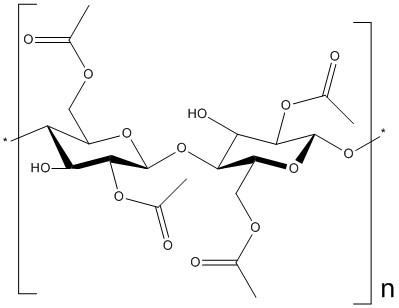
\includegraphics[width=0.7\columnwidth, keepaspectratio]{4-cbs/figs/cellulose_acetate.jpg}
    \caption{Structure of cellulose acetate.}
    \label{fig:cellulose acetate}
\end{figure}

\begin{sloppypar}
The reported porosity of carbons derived from \acrshortpl{ucb} is highly varied depending on synthetic conditions. In the absence of an \gls{activating agent}, and without pre-carbonisation steps, $A_{BET}$ typically does not exceed \qty{700}{\metre\squared\per\gram}.\citep{Koochaki2019, Soltani2013, Yazdi2012, Lee2014, Hamzah2017} Whereas using a \gls{porogen}, and/or pre-carbonising in air or hydothermally can improve surface areas to around \qty{3000}{\metre\squared\per\gram}.\citep{Xiong2018a, Koochaki2019, Sun2017, Bilge2019} The author's reports of ultrahigh porosity from KOH-activated hydrothermally carbonised \acrshortpl{ucb} in \ref{pub:CB} ($A_{BET}$ \qty{>4000}{\metre\squared\per\gram}, pore volume \qty{>2.00}{\cm\cubed\per\gram}) and high degree of microporosity (\qty{>90}{\percent}) are partially corroborated by the similar results using pure \acrfull{ca} in \ref{pub:CA}, suggesting that \acrshort{ca} is an ideal precursor for activation to yield high surface area carbons. Xiong \textit{et al.} also report a nitrogen-doped \acrshort{ucb}-derived activated carbon with hierarchical porosity and $A_{BET}$ of \qty{3420}{\metre\squared\per\gram}, though this result is dubious as (i) the \ce{N2} isotherm does not include ultralow pressure data, (ii) freespace appears to be incorrectly measured and (iii) isotherm measurement is not described in the text.\citep{xiong2019nitrogen} It was suggested in \ref{pub:CB} that the unusually high porosity of \acrshort{ucb}-derived carbons may be contributed to by the action of so-called contaminant-\glspl{porogen}, i.e. trace elements found in cigarette butts that can act as \glspl{activating agent} because carbons from \acrshortpl{ucb} had greater porosity than unused, i.e. `fresh' \acrshortpl{cb}. However, another factor may be the specific treatment of the \acrshortpl{ucb} prior to any carbonisation - that is the removal of any paper, residual ash and tobacco.
\end{sloppypar}

The trace element composition of \acrshortpl{ucb} have been studied by various means, including neutron activation analysis of the intact butts,\citep{iskander1992multielement, Iskander1985, jenkins1985neutron, Wu1997} \gls{adsorption} and emission spectroscopy of various aqueous extracts,\citep{MussaloRauhamaa1986, Kazi2009, Moriwaki2009, Moerman2011, Pelit2013, Dobaradaran2018} voltammetry experiments,\citep{Nitsch1991, Kalcher1993} as well as mixed methods according to environmental contaminant quantification standards.\citep{cardoso2018exposure} The reported concentration has a great degree of variability depending on collection site, method, and brand. For example, work by Iskander \textit{et al.} indicates that \ce{Al} can be present in concentrations as low as \num{59}, and as high as \qty{2200}{\micro\gram\per\gram}, depending on the country of origin of the smoked cigarette butt. Similarly, \acrshort{ucb} samples collected from the environment\citep{Dobaradaran2017, Moriwaki2009, Moerman2011, chevalier2018nano} may have lower quantities of some elements due to leaching, but simultaneously may absorb some elements from the environment (for example from sea water). Trace elements have been identified in \acrshortpl{ucb} from almost every region of the periodic table, including alkali and alkaline earth metals;\cite{MussaloRauhamaa1986, Iskander1985, iskander1992multielement, jenkins1985neutron, Wu1997, cardoso2018exposure}  transition metals, post transition metals and metalloids;\citep{MussaloRauhamaa1986, Dobaradaran2017, Iskander1985, jenkins1985neutron, Wu1997, Moriwaki2009, Moerman2011, Pelit2013, Dobaradaran2018, Ren2017, cardoso2018exposure, chevalier2018nano} lanthanides;\citep{iskander1992multielement} and halogens.\citep{Iskander1985, iskander1992multielement, jenkins1985neutron, Wu1997} Cigarette butt derived carbons have been also been found to contain various metals in trace quantities,\citep{Soltani, Soltani2013, Yazdi2012} although \ce{Ti}, \ce{K}, and \ce{Na} have also been reported at quantities above \qty{1}{\wtpercent}.\citep{Soltani, Soltani2013, Yazdi2012, lima2018, Lee2014} In addition the presence of \ce{Ca}, \ce{K}, \ce{Mg}, \ce{Na}, and \ce{Al} were identified in \acrshort{ucb}-derived \gls{hydrochar} reported in \ref{pub:CB}.

\subsection{Impregnation Methods}

Most commonly in the synthesis of activated carbons \glspl{porogen} are added to precursors by physical mixing - i.e. some combination of grinding and stirring - with the precursor.\citep{Aljumialy2020Porous, Blankenship2017Cigarette, Altwala2020Predictable, Sevilla2016Highly} As mentioned in an alternative technique is to impregnate the precursor with a (typically aqeuous) solution of \gls{porogen}.\citep{Botome2017Preparation, Ge2019Highly, Adlak2021Physicochemical, Shi2021Copper, Han2021Mulch} While there is scant evidence that solution impregnation has better outcomes over physical mixing in terms of porosity development, the rationale of the former technique is that the \gls{activating agent} will be more evenly distributed throughout the precursor thus providing more homogenous porosity in the product however there is as yet no study to support this. 

A further method using oxidative chemical activation is so-called organic salt carbonisation wherein the metal cation of an organic salt activates the carbonised precursor on pyrolysis. Reports, in particular from Sevilla \textit{et al.} show that this method allows for a high degree of tunability in carbon PSDs by changing the identity of the activating cation.\citep{Sevilla2013general, Tsumura2014Structure, Ferrero2015Mesoporous, Ferrero2016Efficient, Fuertes2015Hierarchical, Roberts2015Hierarchically, Yadav20123D, Yang2018Spontaneous} The majority of anions used in organic salt carbonisation are small molecules such as gluconate or citrate,\citep{Sevilla2013general, Yang2017Template, Sevilla2014Direct, Tsumura2014Structure, Ferrero2015Mesoporous, Ferrero2016Efficient, Fuertes2015Hierarchical, Yang2020Production, Fuertes2014One} however polymers have also been employed.\citep{Puthusseri20143D, Roberts2015Hierarchically, Yadav20123D, Hines2004Surface} 

The philosophy of these two emergent techniques (solution impregnation and organic salt carbonisation) for porogen-precursor mixing is that (i) the process can be simplified, (ii) porosity can be more readily controlled, and (iii) porosity is more homogeneous throughout the product. These effects are supposedly a result of both improved \gls{porogen}-precursor contact, and more homogeneous \gls{porogen} distribution. For the purposes of this chapter, mixing techniques with such goals are collectively termed `impregnation' methods. In terms of solution impregnation, thus far syntheses have only been reported wherein the precursor is mixed with the \gls{porogen} directly prior to pyrolysis.\citep{Botome2017Preparation, Ge2019Highly, Adlak2021Physicochemical, Shi2021Copper, Han2021Mulch, Boujibar2018CO2} That is, it has not been attempted to impregnate the \gls{porogen} at the \gls{htc} step. As such, herein the combined \gls{htc} and impregnation of \ce{KOH} on sawdust is examined. This technique is also inspired by the observation made by Zhang \textit{et al.} that the formation of \ce{K} salts with oxygen-rich moieties on the surface of calcined glucose is associated with improvements in ultramicroporosity.\citep{Zhang2019situ} \acrfull{sd} was chosen due to the high quantity of literature surrounding carbons derived from the activation of hydrothermally carbonised sawdust,\citep{Balahmar2019Pre, Aljumialy2020Porous, Cox2017Ultra, Balahmar2015Generalized} making for easy comparison between the results of the technique studied in this chapter and more established techniques.

\begin{figure}[ht!]
    \centering
    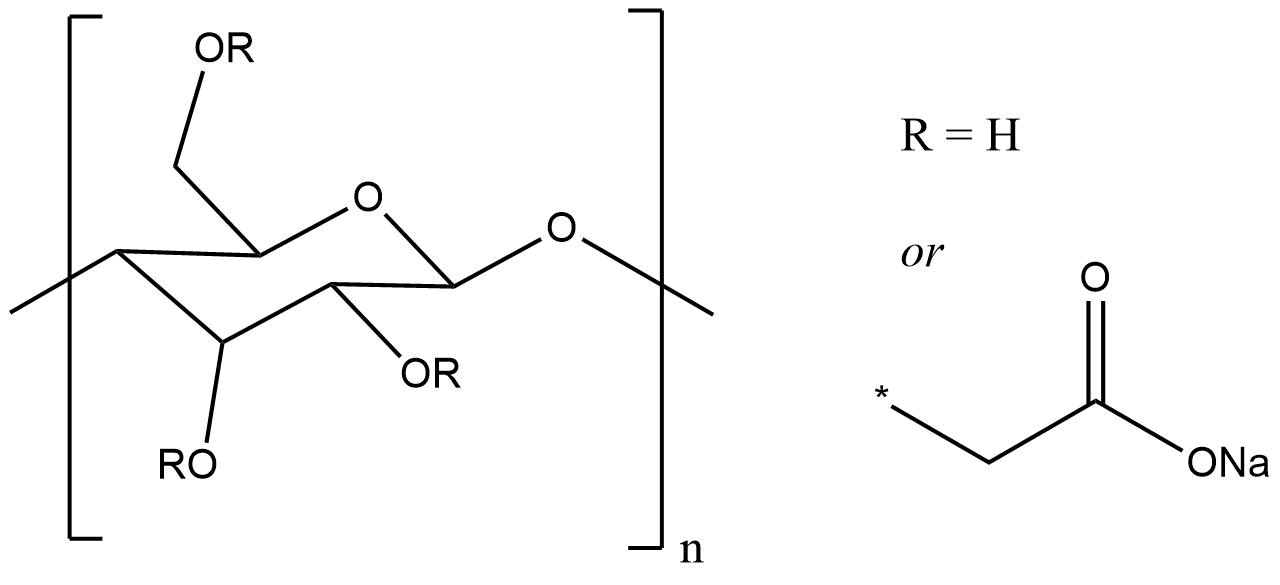
\includegraphics[width=0.8\columnwidth]{4-impregnation/figs/nc_structure.png}
    \caption{Structure of sodium carboxymethyl cellulose. \Acrfull{ds} is taken as the average number of sodium carboxymethyl groups (\ce{-CH2COONa}) per monomer.}
    \label{fig:nc_structure}
\end{figure}

On the other hand, while the porosity of carbons derived through organic salt carbonisation has been exploited through changing the cation,\citep{Sevilla2013general, Tsumura2014Structure, Ferrero2015Mesoporous, Ferrero2016Efficient, Fuertes2015Hierarchical, Roberts2015Hierarchically, Yadav20123D, Yang2018Spontaneous} the capacity for greater more precise control over porosity by changing the degree of substitution of a cation on a polymer chain has not yet been explored. In studies using physical mixing, the \gls{porogen}:precursor weight ratio is typically reported.\citep{Altwala2020Predictable, Adeniran2015Compactivation, Blankenship2017Cigarette, Sevilla2016green, Ludwinowicz2015Potassium, Deng2015Inspired, Alhamed2015Preparation, Hu2003simple} Oxidative chemical activation primarily relies on redox reactions between \ce{C} and the \gls{porogen}, thus knowing the exact stoichiometric  \gls{porogen}:\ce{C} ratio may provide a route to understanding the precise effects of \gls{porogen} concentration on carbon porosity requires information as to the composition of the precursor. To this end, this study also investigates \acrfull{nc} (structure shown in figure \ref{fig:nc_structure}) as a precursor to activated carbon. The \gls{porogen} in this case is the sodium carboxymethyl group, and the \gls{porogen}:precursor ratio is controlled by the \acrfull{ds}.

\section{Physisorption \& porosity}
\label{s:adsorption_porosity}
Porous materials possess an interconnected pore system where pores are defined as voids which are deeper than they are wide.\citep{mcnaught1997compendium, Thommes2015Physisorption} Additionally, pores are defined as being able to contain fluid, which indirectly gives a minimum width for voids to be considered pores of \qty{2.6}{\angstrom}, as this is the kinetic diameter of the smallest practical fluid specie, \ce{He}.\citep{Thommes2015Physisorption, Lide2007Handbook} The ability of porous materials to contain fluids has led to the use of the phenomenon of adsorption being used to characterise their porosity. That is, knowledge of the behaviour of the system when the material is enriched with a fluid is utilised to understand pore size, shape and interconnectivity. In particular, so-called \gls{physisorption} is exploited wherein \gls{adsorbate}-\gls{adsorbent} interactions do not include any sort of chemical attraction but instead rely on non-bonding forces\citep{Thommes2015Physisorption} - thus hypothetically, structure ought not be significantly conflated with surface chemistry. What follows is a discussion of the various types of pore structures and associated adsorption phenomena, and thus an overview of methods to determine porosity from an isotherm.

\subsection{Pore characteristics and filling mechanisms}
\label{ss:pore_filling}

The \acrfull{iupac} defines ranges of pore sizes according to the mechanisms of pore filling by an \gls{adsorbate}.\citep{Thommes2015Physisorption} The three main mechanisms; \gls{micropore} filing; monolayer adsorption; and multilayer adsorption are illustrated in figure \ref{fig:filling}. Specifically, \glspl{micropore} (\qty{<20}{\angstrom})\citep{mcnaught1997compendium} are filled at ultralow relative pressures, and are characterised by strong heats of adsorption due to complementary \gls{adsorbate}-\gls{adsorbent} interactions from all pore walls.\citep{dubinin1989fundamentals} The subdivision into \glspl{ultramicropore} (\qty{<7}{\angstrom}) and \glspl{supermicropore} (\qtyrange[range-units=single]{7}{20}{\angstrom})\citep{mcnaught1997compendium} is derived from the fact that pores narrower than \qty{7}{\angstrom} can fit two adjacent rows of \ce{N2} molecules,\citep{Thommes2015Physisorption} and thus have the highest degree of pore wall potential overlap. \Glspl{mesopore} (\qtyrange[range-units=single]{20}{500}{\angstrom})\citep{mcnaught1997compendium} are characterised by being large enough to allow monolayer adsorption. That is, all adsorbed molecules are in contact with the surface and are not significantly influenced by attraction to an opposing pore wall.\citep{gregg1967adsorption, yang1997gas} As pressure increases, repulsive \gls{adsorbate}-\gls{adsorbate} interactions are overcome so that additional \gls{adsorbate} molecules adsorb on top of the monolayer - this process is known as multilayer adsorption. The widest pore size classification is \glspl{macropore} which are larger than 500 \unit{\angstrom}\citep{mcnaught1997compendium} and are not easily characterised by isothermal gas adsorption experiments, instead necessitating the use of mercury intrusion porosimetry for determination of porosity.\citep{abell1999mercury, gregg1967adsorption, haynes1973pore} In addition to these principal adsorption processes, in \glspl{mesopore} capillary condensation can occur at relative pressures greater than \num{\sim0.2} wherein the adsorbate enters a liquid-like state despite being below saturation pressure. This can lead to hysteresis in the resultant isotherm which is discussed in more depth in section \ref{ss:iso_interpretation}.\citep{Thommes2015Physisorption, monson2012understanding}

\begin{figure}[ht!]
    \centering
    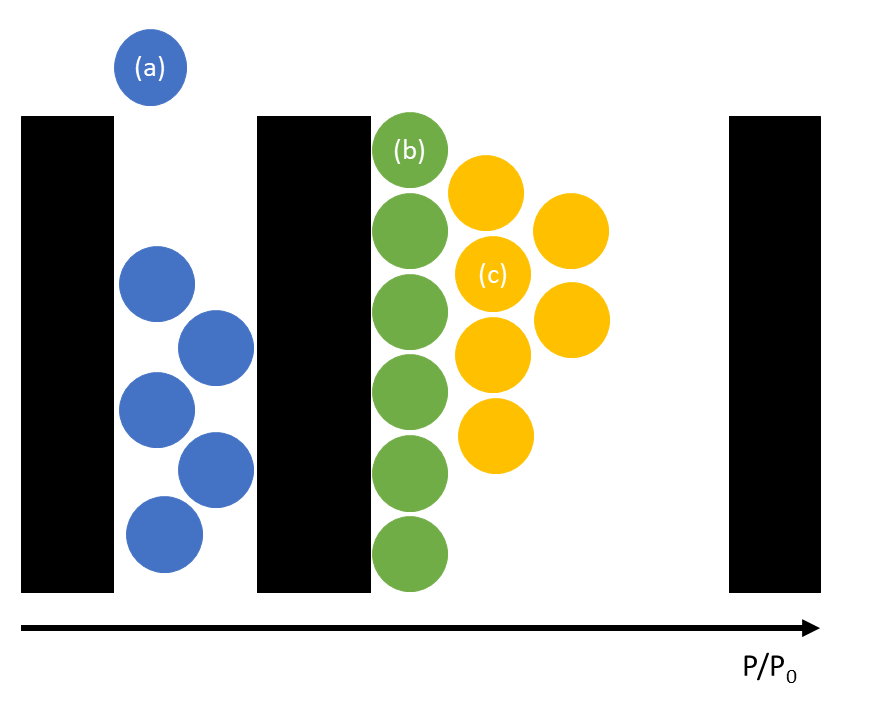
\includegraphics[width=\columnwidth, keepaspectratio]{1-introduction/figs/pore_filling.png}
    \caption{The three principle pore filling mechanisms, in order of their occurence with increasing relative pressure; (a) micropore filling; (b) completion of the monlayer in mesopores; and (c) multilayer adsorption.}
    \label{fig:filling}
\end{figure}

While few materials show uniform pore shape, idealised shape is defined by \acrshort{iupac} according to five characteristic shapes; cylindrical, slit, funnel, sphere, and ink-bottle.\citep{rouquerol1994recommendations, kaneko1994determination, zdravkov2007pore} For example while aluminium oxides typically have cylindrical pores,\citep{zdravkov2007pore} \glspl{turbostratic carbon} are usually assumed to have slit-shaped pores,\citep{Everett1976Adsorption, Jagiello20132D, Lastoskie1993} although carbide-derived carbons have been shown to possess cylindrical or spherical pores.\citep{kurig2016suitability} Zeolites have a broad range of pore shapes.\citep{park2002effect} 

\begin{figure}[b!]
    \centering
    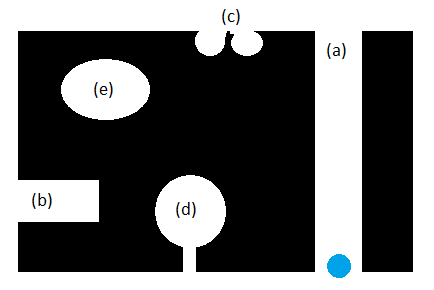
\includegraphics[width=\columnwidth, keepaspectratio]{1-introduction/figs/pore_accessibility.png}
    \caption{The different types of pores classified according to their accessibility; (a) an open, through pore; (b) an open, blind pore; (c) external pores; (d) a chemically closed pore; and (e) a closed pore. The small blue dot indicates the probe molecule size.}
    \label{fig:pore_accessibility}
\end{figure}

In addition to shape and size, pores are also defined by their degree of accessibility. Figure \ref{fig:pore_accessibility} illustrates this type of pore classification. In general, pores can be termed as `closed' or `open', based on whether or not they have an accessible entrance. In the case of open pores, these are further subdivided into `through' pores wherein both ends of the pore are accessible, and `blind' pores wherein only one end of the pore is accessible. In addition, porosity can be formed through undulations on the surface, provided that the depth of these undulations is greater than the width. These are known as `external pores'. However open pores are not necessarily accessible to an adsorptive, that is there entrance may be smaller than the adsorptive molecule - these pores are termed as `chemically closed'. This can occur for ink-bottle pores with a narrow neck, or for very narrow slit or cylindrical pores.\citep{rouquerol1994recommendations, kaneko1994determination, zdravkov2007pore} Porosimetry is only able to quantify apparent porosity as defined by `true' open pores (i.e. not chemically closed) and indeed for gravimetric adsorption applications this is the the only kind of meaningful porosity. However, closed pores nonetheless contribute to a materials bulk density and thus can influence \textit{volumetric} uptake capacity for an adsorptive.


The final characteristic of porous structures is porosity hierarchy. Materials like \acrshortpl{mof} and zeolites typically possess uniform or unimodal porosity,\citep{WeitkampZeolites, Siriwardane2005Adsorption, Ding2019Carbon, lin2009hydrogen} whereas \glspl{turbostratic carbon} typically have multiple- or even a continuous range of (i.e. hierarchical) pore widths.\citep{Li2020Hierarchical, Sevilla2014Energy, Xia2008Hierarchical, Balahmar2017Biomass} The pore hierarchy or lack thereof can play an important role in which applications the material is best suited to - for example a uniform \acrfull{psd} can be used to exclude molecules of a certain size.\citep{qian2020mof, reid2001adsorption, Adeniran2014family}

\subsection{Isotherm classification and interpretation}
\label{ss:iso_interpretation}

The various adsorption behaviours of a porous material discussed in the previous section result in distinct and interpretable forms of the resultant isotherms. As a general rule, the relative amount of gas adsorpted in different pressure ranges gives an indication of the amount of porosity in the internal \gls{micropore} and \gls{mesopore} regions as well as the amount of external surface area. To demonstrate, a labelled isotherm is shown in figure \ref{fig:isotherm_anatomy}. High adsorption in the low pressure region indicates the presence of \glspl{micropore}, while an increase in uptake at pressures around the midpoint of the isotherm indicate mesoporosity. If there is a plateau in the middle of the isotherm, this typically indicates that a monolayer has formed. The curvature of the isotherm prior to the plateau (the adsorption `knee') is indicative of the breadth of the \acrshort{psd}; a gentle knee shows a broad \acrshort{psd}, while a sharp knee indicates that pore sizes are narrowly distributed. Finally, high uptake as relative pressure approaches 1 are indicative of adsorption on the external surface, showing that the material is non-porous or macroporous.\citep{Thommes2015Physisorption} \acrshort{iupac} has designated eight distinct isotherm types.\citep{Thommes2015Physisorption, Sing1985} These need not be discussed in full detail here - it is sufficient to state that types I(a) and (b) isotherms are indicative of microporosity, while IV(a), IV(b) and V are seen on isotherms with high mesoporosity. Nonporous samples typically exhibit type II, III or VI isotherms. The variation in shapes can be indicative of surface chemistry and/or pore size hierarchy.\citep{thommes2014physical, monson2012understanding} Of course as a lot of materials exhibit multiple types of porosity, many materials exhibit characteristics of multiple isotherm types.\citep{Thommes2015Physisorption} 

\begin{figure}[t!]
    \centering
    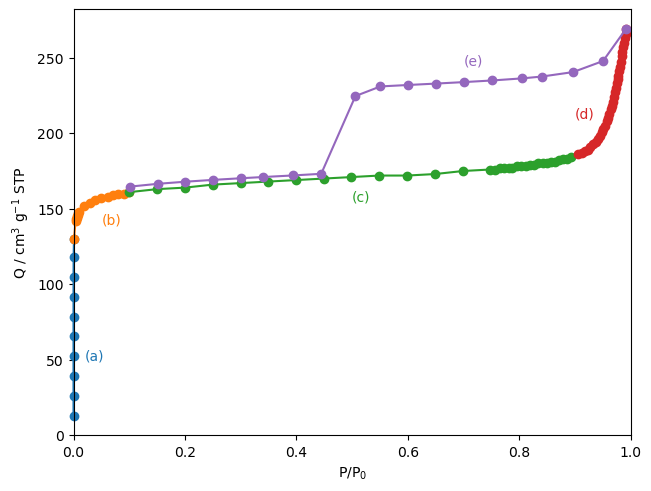
\includegraphics[width=\columnwidth, keepaspectratio]{1-introduction/figs/isotherm_anatomy.png}
    \caption{An isotherm of \ce{N2} on a turbostratic carbon. The isotherm possesses (a) high uptake in the micropore region, indicating microporosity; (b) a sharp knee due to a narrow \acrshort{psd}; (c) a plateau in the medium pressure region due to formation of a monolayer this remains flat in the middle of the isotherm due to lack of mesoporosity; (d) high uptake as relative pressure approaches 1 showing external surface adsorption; and (e) a hysteresis loop due to capillary condensation.}
    \label{fig:isotherm_anatomy}
\end{figure}

Apart from the general isotherm types, the presence of hysteresis - i.e. desorption releasing less \gls{adsorbate} than is taken up during adsorption at an identical relative pressure - is indicative of capillary condensation (see section \ref{ss:pore_filling}.\citep{thommes2014physical, monson2012understanding, landers2013density} As with characteristic isotherm types, \acrshort{iupac} has defined six distinct forms of hysteresis loop. Depending on the type of hyteresis loop, its presence may indicate adsorption metastability in an `open' pore, pore network effects and/or other forms of pore blocking.\citep{Thommes2015Physisorption} Each of the six hysteresis loops are associated with specific kinds of materials - for example H4 loops are frequently found in micro-mesoporous carbons, whereas H1 is typically associated with materials possessing uniform open mesopores.\citep{Thommes2015Physisorption, monson2012understanding}  

\subsection{Isotherm models}

The theory of adsorption on a surface can be described mathematically, that is loading of \gls{adsorbate} on an \gls{adsorbent}, $Q$ can be described as a function of pressure, $p$. In the simplest instance, Henry's law\citep{henry1803experiments} (equation \ref{eq:henry} can be used to described a linear relationship.

\begin{equation}\label{eq:henry}
    Q(p) = K_H P
\end{equation}

Of course, a linear relationship is unrealistic as saturation eventually occurs. Nonetheless, $K_H$ an be used as an approximation of the strength of interaction between \gls{adsorbate} and \gls{adsorbent}. Improvements can be attained through treating the isotherm as a quadratic or virial function, or by the Freundlich approach which modifies the Henry equation to account for the unavailability of adsorption sites by with increase in loading by using the exponent $\frac{1}{m}$, but this still does not account for saturation. Furthermore, neither of these approaches consider the specific case of adsorption of gases onto solid surfaces. Such a theory was first introduced by Langmuir using kinetics. This assumes a reversible reaction between an ideal \gls{adsorbate}, $A_g$ and an \gls{adsorption} site, $S$ to form the adsorbed complex, $A_{ad}$. The reaction proceeds until it reaches equilibrium with constant $K$;

\begin{equation}
    \ce{A_g + S <=>[K] A_{ad}}
\end{equation}

From this can be derived the Langmuir isotherm (equation\ref{eq:langmuir}), which also accounts for the formation of the monolayer which under this theory is the maximum possible loading, by including the monolayer capacity, $Q_m$.

\begin{equation}\label{eq:langmuir}
    Q(P) = n_m \frac{K P}{1 + K P}
\end{equation}

This can then be adapted to account for \gls{adsorbent} heterogeneity by considering multiple \gls{adsorption} sites, each with their own equilibrium constants, $K_i$ and monolayer capacities $Q_{m_i}$. Thus the isotherm is modelled as a summation of Langmuir isotherms as in equation \ref{eq:multi_langmuir}. Alternatively, as in the T\'{o}th model, a heteroegeneity factor, $t$ can be used - see equation \ref{eq:toth}. 

\begin{equation}\label{eq:multi_langmuir}
    Q(P) = \sum_{1} Q_{m_i} \frac{K_i P}{1 + K_i P}
\end{equation}

\begin{equation}\label{eq:toth}
    Q(P) = n_m \frac{K P}{\sqrt[t]{1 + (K P)^t}}
\end{equation}

Thus, surface heterogeneity can be quantified by $t$ or the number of adsorption sites. In addition, it has been recently shown that equilibrium constant(s) can be use to approximate the potential energy of adsorption, $\varepsilon$ as a function of surface coverage (i.e. fractional loading).\citep{whittaker2013predicting} On the other hand, the  Dubinin-Radushkevitch and later the Dubinin-Astakhov (see equation \ref{eq:da}) models explicitly considers the thermodynamics of adsorption and so $\varepsilon$ is included in such a treatment.

\begin{equation}\label{eq:da}
    Q(P) = Q_m \exp{ \left[ - \left( \frac{ -R T \ln{\left( \frac{P}{P_0}\right)}}{\varepsilon} \right) \right]^m }
\end{equation}

What is lacking in all of the models discussed above is a description of multilayer adsorption. Stephen Brunauer, Paul Emmet, and Edward Teller expanded Langmuir theory to account for multilayer \gls{adsorption}, which occurs at higher pressures and temperatures. The following assumptions are made;\citep{Brunauer1938Adsorption}

	\begin{enumerate}[label=(\arabic*)]
		\item Gas molecules adsorb on solid layers infinitely;
		\item Gas molecules only interact with adjacent layers;
		\item The Langmuir theory can be applied to each layer.
		\item The enthalpy of \gls{adsorption} for the first layer is constant and greater than that for subsequent layers;
		\item After monolayer \gls{adsorption}, the enthalpy of \gls{adsorption} is the same as that of liquefaction.
	\end{enumerate}

The total quantity of gas adsorbed, $Q$  and thus the proportional surface coverage, $\theta$ is related the quantity of the monolayer, $Q_m$ by equation \ref{eq:bet}. This contains the constant $c$ which describes (see equation \ref{eq:bet_c}) the difference in heats of adsorption, $\lambda$ between the first and subsequent layers. The latter is assumed to be the heat of liquefaction $\lambda_L$.

\begin{equation}\label{eq:bet}
    \theta(P) = \frac{Q}{Q_m} =  Q_m \frac{c P}{\left( 1 - \frac{Q}{Q_0} \right) \left(P_0 + P \left(c - 1 \right) \right)}
\end{equation}

\begin{equation}\label{eq:bet_c}
    c = \exp{\frac{\lambda_1 - \lambda_L}{RT}}
\end{equation}

Equation \ref{eq:bet} can be rearranged to give equation \ref{eq:bet_plot}, which yields a linear relationship. When applied to an iostherm both the thermodynamic constant $c$ and the monolayer loading, $Q_m$ can be derived. From the former the enthalpy of monolayer adsorption can be calculated. The latter gives a simple method (equation \ref{eq:bet_area} )to quantify the specific surface area of the \gls{adsorbent} if the cross-sectional area of the \gls{adsorbate}, $\sigma$ is known.

\begin{equation} \label{eq:bet_plot}
    \frac{1}{Q  \left( \frac{P_0}{P} - 1 \right)} = \frac{c-1}{Q_m \, c}  \left( \frac{P}{P_0} \right) + \frac{1}{Q_m \, c}
\end{equation}

\begin{equation}\label{eq:bet_area}
    A_{BET} = \frac{Q_m \, N_A \, \sigma}{a}
\end{equation}

Where $N_A$ is the Avogadro constant and $a$ is the mass of the \gls{adsorbent}.\citep{Brunauer1938Adsorption} In equation \ref{eq:bet_area}, calculation of the \acrshort{bet} area per unit mass of \gls{adsorbent} is shown. It can also be written in terms of total area, or \gls{adsorbent} volume given the density of the \gls{adsorbent}.

For microporous materials, using the \acrshort{bet} method to calculate surface area is problematic for two reasons;

	\begin{enumerate}[label=(\arabic*)]
		\item The initial step in the \gls{adsorption} mechanism is not the formation of the monolayer, but the filling of \glspl{micropore}. This renders \acrshort{bet} theory inaccurate for microporous materials.
		\item 	Following the \acrshort{bet} transform, there are often multiple linear regions of the plot. This means that reported $A_{BET}$ may be inconsistent.
	\end{enumerate}

Despite these problems, $A_{BET}$ continues to be the dominant measure of surface area used for microporous materials. As yet, there is no widespread alternative or extension of \acrshort{bet} theory that solves (1), however the standardisation required according to (2) is most commonly achieved according to a method described by Rouquerol et al, where the \acrshort{bet} plot is transformed by changing the term on the y-axis to $Q \left(1 - \frac{P}{P_0} \right)$. This yields a roughly parabolic graph known as the Rouquerol transform. A pressure range of the \acrshort{bet} transform can then be selected to yield a consistent calculation of $A_{BET}$ according to the following principles;

	\begin{enumerate}[label=(\arabic*)]
		\item The intercept of the original \acrshort{bet} transform must be positive, as a negative intercept would yield a negative value for $c$.
		\item The range selected must correspond to a region of the Rouquerol transform where $Q \left(1 - \frac{P}{P_0} \right)$ constantly increases with $\frac{P}{P_0}$.
		\item $Q_m$ as determined from (1) and (2) can be found in the region of the isotherm selected.\citep{Rouquerol2007Is} 
	\end{enumerate}

There have been further modifications to the \acrshort{bet} theory including \acrfull{gab}, which attempts to account for the differences in enthalpies of adsorption and liquefaction.\citep{Guggenheim1966Applications} Other extensions to \acrshort{bet} theory have been developed to give a more realistic model of adsorption for example by including the fact that number of layers adsorbed ought to be finite, or by substitution of relative pressure for relative density of the adsorbed phase which is useful in the case of for supercritical isotherms.\citep{Brunauer1940, zhou2019modified}

\subsection{Pore size distributions}

As detailed in section \ref{ss:iso_interpretation}, isothermal porosimetry can be used to determine a general qualitative definition of the porosity of a sample. Due to the development of models of adsorption, this can further be expanded to quantify porosity. In the first instance, scalar quantities such as pore volume or surface area can be determined.\citep{Thommes2015Physisorption} The simplest example of the former is the single point pore volume which relies simply on the amount adsorbed at the isothermal plateau for a subcritical \gls{adsorbent} as saturation is approached. As for surface area, this is most commonly determined from BET theory and/or Langmuir theory.\citep{Brunauer1938Adsorption, Langmuir1918adsorption} Further theoretical manipulations such as t-plot or Dubinin treatments can be used to determine porosity within some range, i.e. \glspl{micropore} or \glspl{mesopore}.\citep{Dubinin1971Description, Marczewski2002practical} Alternatively a supercritical isotherm can be used to find pore volume below a certain maximum pore width, with the adsorbate and conditions selected to exclude pores larger than some maximum. A common example of this is \ce{CO2} at \qty{0}{\degreeCelsius} to find pore volume in pores smaller than \qty{10}{\angstrom}.\citep{Jagiello2019Enhanced, Sevilla2013Assessment, Thommes2015Physisorption} Porosity can also be defined using a vector, namely the \acrfull{psd} which is essentially the porosity of the sample as a function of pore width typically represented as $f(w)$. Typically porosity is defined as pore volume but can easily be converted to be in terms of surface area. The resulting relationship can be used in the form of an incremental or cumulative \acrshort{psd}. While incremental \acrshortpl{psd} can be used to determine discreet pore widths, its cumulative counterpart is useful for finding the volume of pores within some range of widths such as \glspl{micropore}. By this token, the \acrshort{psd} can also be used to determine total pore volume or surface area.\citep{Thommes2015Physisorption, shull1948physical, Barrett1951determination}

Classical models used for determining \glspl{psd} rely on parameters including the monolayer capacity of the \gls{adsorbent}, as well as the \gls{adsorbate}-\gls{adsorbent} interaction. Additionally, they make use of false assumptions such as that the \gls{adsorbate} behaves as a two-dimensional ideal gas (in the case of the Horvath-Kawazoe model).\citep{Barrett1951determination, Horvath1983Method}  A more recent development method is the kernel fit \acrshort{psd}, wherein the experimental isotherm is fit to a library (the kernel) of model isotherms that vary only according to the single pore width of the \gls{adsorbent}.\citep{Thommes2015Physisorption, tan1990adsorption, sosin1995using, tarazona1987phase} The determination of isotherms in the kernel relies on statistical modelling of \gls{adsorbate}-\gls{adsorbate} and \gls{adsorbate}-\gls{adsorbent} interactions specific to a system defined by pore size, pore geometry, the adsorptive and temperature. As a result, the \acrshortpl{psd} determined this way are much more accurate. The determination of the kernel is most commonly performed using \acrfull{dft} or \acrfull{gcmc} computational methods. Currently, \acrshort{dft} methods are preferred and are discussed below.

In the simplest method to calculate a kernel, a system is described by a surface with single width, slit shaped pores under vacuum. This is then dosed with argon at a specified pressure. As this occurs argon atoms will begin to fill the pore, causing pressure in the bulk \gls{adsorbate} to decrease until an equilibrium is reached between the bulk argon and that adsorbed within the pore. According to the theory of dispersion interactions, the argon should be most concentrated at the surface at equilibrium – this concentration is the amount of gas adsorbed at the given pressure, i.e. one point on an isotherm. The amount of gas adsorbed can be calculated by minimising the free energy of the system as given by the Lennard-Jones potential, $U(s)$;

\begin{equation}
U(s) = 4\varepsilon \left[ \left(\frac{\sigma}{s}\right)^{12} -  \left(\frac{\sigma}{s}\right)^{6} \right]
\end{equation}

Where $s$ is the distance between the \gls{adsorbate} and surface, $\varepsilon$ is the energy of the \gls{adsorbate}; and $\sigma$ is the molecular diameter of the \gls{adsorbate}.  Thus, by varying the pressure from ultra-low to saturation, the amount of gas adsorbed at defined pressures can be calculated, and from this a model isotherm of this simple theoretical system can be built. 

In practice, the equilibrium density profile is built up by minimising the grand potential energy of the system as a function of density, $\Omega[\rho(r)]$ - which is calculated for a point $r$ in the system as follows;

\begin{equation}
\Omega[\rho(r)] = F[\rho(r)] + \int \rho(r)\left(V(r) - \mu\right) \,\rm{d}r
\end{equation}

The rightmost, integral term defines the gas properties via the ideal gas equations according to the potential acting on the molecule $V(r)$, while $F[\rho(r)]$ is the Helmholtz free energy of the gas at equilibrium density at point $r$. $F[\rho(r)]$ is defined by the sum of repulsive (hard sphere) and attractive interactions between gas molecules. This treatment results in the local density approximation, which assumes that a local part of an inhomegeneous system has the same free energy density as a bulk homogeneous system of the same density. The inaccuracy of this treatment has led to further development of the theory via non-localised methods (\acrfull{nldft}), \citep{tarazona1987phase, lastoskie1993pore, landers2013density} and further extended using a corrugated pore model to account for energetic heterogeneity, as developed by Jagiello et al.\citep{Jagiello20132D} These adaptations are discussed in greater depth below.

Regardless of the method, the computational generation of an isotherm is repeated across a range of pore widths to generate a library of isotherms for a specific \gls{adsorbate}-\gls{adsorbent} system known as the kernel, $N\left(\frac{P}{P_0}, \, W\right)$. The general \gls{adsorption} integral equation (equation \ref{eq:GAI}) is then used to correlate the experimental isotherm, $N\left(\frac{P}{P_0}\right)$  with the kernel resulting in the pore size distribution as a function of pore width, $f(W)$.\citep{Thommes2015Physisorption}

\begin{equation} \label{eq:GAI}
    N\left(\frac{P}{P_0}\right) = \int_{w_{min}}^{w_{max}} N\left(\frac{P}{P_0}, \, w \right) f(W) \, \mathrm{d}w
\end{equation}

This data can be displayed in terms of differential or cumulative pore volume and surface area, and as such can be used to determine textural quantities which prior to the development of kernel-fit \acrshortpl{psd} had been calculated \textit{via} classical methods.

The earliest kernels for \gls{adsorption} of \ce{N2} on porous carbon used a one-dimensional, homogeneous, semi-infinte model of the pore wall surface.\citep{seaton1989new} That is, the pore wall is completely flat and its length extends to infinity. This simplified kernel determination as pore space was only characterised by the pore width, and used a local density approximation to account for repulsive forces; short-range interactions are omitted for simplicity. Unfortunately this results in a poor description of the density profile of \gls{adsorbate} molecules near the pore walls. Tarazona and co-workers improved on this model by considering these short-range interactions, producing the so-called \acrfull{nldft} kernel.\citep{tarazona1985free, tarazona1987phase} This nonetheless does not consider the energetic and chemical heterogeneity of pore walls within real porous carbons. Not only is this inaccurate, but the use of these kernels leads to poor fitting to the experimental isotherm and consistent artefacts in the resultant \acrshort{psd}.\citep{Jagiello20132D,  olivier1998improving, lueking2009tests, nguyen2004characterization} Olivier suggested improvements such as applying weightings to the model isotherms before fitting to the experimental data, as well as using a finite pore model.\citep{olivier1998improving} Nguyen and Bhatia found some improvements by taking the approach of considering pore wall heterogeneity by varying the pore wall thickness.\citep{nguyen2004characterization} Jagiello \textit{et al.}, however consider the pore wall to be a two-dimensional surface, having regular sinusoidal corrugations. This accounts for both chemical and energetic heterogeneity\citep{Jagiello20132D} and the eponymous 2D-NLDFT-HS (2-dimensional NLDFT heterogeneous surface) approach results in a better fit to the experimental isotherm.\citep{Jagiello20132D, puziy2016comparison, shi2021current} Thus far, the 2D-NLDFT-HS kernel has been developed for \ce{N2}, \ce{O2}, \ce{H2}, \ce{CO2}, and \ce{Ar}.\citep{Jagiello20132D, Jagiello2013, jagiello2019consistency, Jagiello2020Exploiting}

The general \gls{adsorption} integral equation was shown in equation \ref{eq:GAI}. For convenience, it is reproduced in equation \ref{eq:GAI_jagiello} in a form closer to that used by Jagielllo. $V(p_i)$ and $K(p_i,\,w)$ are the experimental isotherm and kernel respectively, and $f(w)$ is the differential \acrshort{psd} to be calculated.

\begin{equation} \label{eq:GAI_jagiello}
    V(p_i) = \int_{w_{min}}^{w_{max}} K(p_i,w) f(w) \, \mathrm{d}w
\end{equation}

The solution to this equation is quite involved, but is achievable using a method developed by Jagiello.\citep{Jagiello1994Stable} In short, a stable \acrshort{psd} can be determined by using the regularization approach to determine an appropriate fitting parameter, $\lambda$\citep{Hansen2001, Hansen1993use, Hansen2001L} and the discrete result is interpolated using the B-spline approach.\citep{knott2000interpolating, prautzsch2002bezier, deboor1978practical} This method is automated in the SAIEUS (Solution to the Adsorption Integral Equation Using Splines) program.\citep{Jagiello1994Stable} The $\lambda$ variable is added to the expression in equation \ref{eq:GAI_jagiello} to produce \ref{eq:GAI_jagiello_lambda};

\begin{equation} \label{eq:GAI_jagiello_lambda}
    V(p_i) = \int_{w_{min}}^{w_{max}} K(p_i,w) f(w) \, \mathrm{d}w + \lambda\int_{w_{min}}^{w_{max}}\left[ f''(w) \right]^2\, \mathrm{d}w
\end{equation}

When considering $M$ multiple isotherms, a summative approach is needed.\citep{caguiat2014uncertainties} Minimisation of the multi-isotherm, multi-kernel  expression in equation \ref{eq:multiple_isotherm} for each \gls{adsorbate}, $m$ will yield a single \acrshort{psd} for all $M$ isotherms.\footnote{The summative expression in equation \ref{eq:multiple_isotherm} is a result of the solution to the single isotherm general \gls{adsorption} integral equation described in equation \ref{eq:GAI_jagiello_lambda}. Its derivation is discussed by Jagiello in the original paper,\citep{Jagiello1994Stable} but is outside the scope of this work.}

\begin{equation} \label{eq:multiple_isotherm}
    \mathrm{min}\sum_{m}^{M}\sum_{i}^{N_m}\left[ V_m(p_i) - \int_{w_{min}}^{w_{max}}K_m(p_i,\,w)f(w)\,\mathrm{d}w\right]^2 + \lambda\int_{w_{min}}^{w_{max}}\left[ f''(w) \right]^2\, \mathrm{d}w
\end{equation}

Where $V_m(p_i)$ and $K_m(p_i,\,w)$ are the $m$th experimental isotherm and $m$th kernel respectively.\citep{Jagiello2015Dual, Jagiello2008Characterization, Jagiello2007}

\section{\texorpdfstring{\ce{CO2} capture}{CO2 capture}}
\label{s:ccs}

Methods for \ce{CO2} capture as an add-on to industrial processes can be divided into three principal, broad groups; (i) oxy-fuel combustion, (ii) pre-combustion capture and (iii) post-combustion capture.\citep{kanniche2010pre} Oxy-fuel combustion is not a true \ce{CO2} capture method, but provides a means to more facile \ce{CO2} capture by producing a highly pure stream of \ce{CO2} meaning that gas separation is not necessary priory to capture.\citep{stanger2015oxyfuel, wall2009overview} Pre-combustion capture on the other hand involves the gasification of the fuel source using steam and oxygen, forming a mixture of \ce{H2} and \ce{CO} which is known as syngas. The \ce{H2} can be used as a fuel, while in a similar manner to oxy-fuel combustion, the \ce{CO} is converted to pure \ce{CO2} for ease of capture.\citep{jansen2015pre} Post-combustion capture does not require any of these complex treatments - \ce{CO2} is simply separated and captured from existing flue streams.\citep{wang2017review, samanta2012post} Thus, this method may be considered the the most versatile of the three.

The principal commercial mode of post-combustion \ce{CO2} capture is \textit{via} chemical capture using liquid amines. This process is plagued by high costs due to the degradation of the amine solvent as well as corrosion of equipment.\citep{aronu2009solvent, dutcher2015amine, delgado2018degradation} Membrane-based \ce{CO2} capture and separation doesn't rely on chemical regeneration as the requisite membrane material simply selectively allows \ce{CO2} to travel through it while excluding other molecules due to their size.\citep{adewole2013current, ramasubramanian2011recent} The (theoretically) pure stream of \ce{CO2} is then captured at the other side. In order for this to work, high pressures must be use to force \ce{CO2} through the membrane; this can often lead to membrane degradation.\citep{powell2006polymeric} As a result of these problems, a third category of \ce{CO2} capture materials is under a lot of investigation - that is, solid porous sorbents which are not plagued by high regeneration costs or degradation. These include \acrshortpl{mof},\citep{Ding2019Carbon, qian2020mof} zeolites,\citep{Siriwardane2005Adsorption, Krishna2010silico} and of course porous carbons.\citep{Zhu2015Naturally, Chen2019Template, Xia2011Superior, Sevilla2016Highly} 

Candidates for solid \glspl{adsorbent} applied to \ce{CO2} capture are typically exploited for swing adsorption processes such as \acrfull{psa}, \acrfull{vsa} or \acrfull{tsa}. This type of process relies on \gls{adsorption} taking place at some pressure (\acrshort{psa}, \acrshort{vsa}) or temperature (\acrshort{tsa}) after which \ce{CO2} can be regenerated by changing the condition; typically this means reducing the pressure or increasing the temperature to facilitate desorption.\citep{bahamon2018energetic, hedin2013adsorbents, Zhao2018Synthesis, adewole2013current, ho2008reducing}  \acrshort{psa} and \acrshort{vsa} only differ in that the former captures \ce{CO2} at elevated pressure and regenerates by reducing to ambient pressure; whereas the latter performs capture at ambient pressure and release occurs at vaccuum. Thus \acrshort{vsa} is more cost effective, however both of these pressure-based solutions are more desirable than \acrshort{tsa} as they can be performed at the elevated temperatures present in flue gases.\citep{ho2008reducing, adewole2013current, Pirngruber2013} Due to the different physical conditions used to capture and regenerate \ce{CO2} in each of these adsorptive processes, selection of solid sorbent is based on porosity. For example, materials for \acrshort{psa} should have a high specific surface area and possess minimal microprosity while for \acrshort{vsa} pore size is more important than overall surface area.\citep{ho2008reducing, Chou2004, Presser2011Effect} Physisorbents such as \acrshortpl{mof} and zeolites have also been recently applied to the newer field of \acrfull{dac}, which may prove a necessary, complementary technology to post-combustion capture.\citep{kumar2015direct, mcqueen2021review, deutz2021life} Selectivity for \ce{CO2} over \ce{N2} is particularly important in \acrshort{dac} due to \ce{CO2}'s low partial pressure in the air. The selectivity is usually facilitated \textit{via} moieties with high chemical affinity for \ce{CO2}, but nonetheless porosity is likely to play a role in the performance of these materials.\citep{kumar2015direct, darunte2016direct, deng2021comparative}

While surface chemistry may play a role in the suitability of a porous carbon to capture \ce{CO2} and indeed the applicability of a porous material in general to adsorb a gas,\citep{Lueking2004, Li2011a, Li2020Sustainable, wang2012significantly, Botome2017Preparation, liang2013, Kayal2018Activated} in the case of \glspl{turbostratic carbon}, porosity is the defining variable for \ce{CO2} capture performance.\citep{Sevilla2014Energy, Adeniran2016Is, Sevilla2013Assessment, Choi2019Unique, Lee2013Determination, Presser2011Effect, Wickramaratne2013Importance}  Simply increasing overall surface area and pore volume does improve gas uptake,\citep{Cox2017Ultra, Blankenship2017Cigarette} however the magnitude of the effects of increasing these parameters are limited by pore size\citep{Sevilla2014Energy, Sevilla2013Assessment, Choi2019Unique, Li2019Selective, Cabria2007optimum, Gogotsi2009, Masika2012} - that is, it is important to maximise the porosity contained within pores of some specific width in order to optimise \ce{CO2} uptake capacity. This so-called optimum pore width is dependent on the surface chemistry\citep{wang2012significantly, Kayal2018Activated, Lueking2004} and pore geometry\citep{Rzepka1998Physisorption, Zhou2004comparative, Hlushak2018Heat} of the \gls{adsorbent}. With all of these factors controlled for, at a given temperature, optimum pore size also appears to be highly variable with pressure.\citep{Presser2011Effect, DelaCasaLillo2002Hydrogen} Up to now, the optimum pore width is defined either as (i) a single pore width\citep{Sevilla2014Energy, Choi2019Unique, Li2019Selective} or (ii) all pores of width less than some maximum.\citep{Biloe2002Optimal, Cabria2007optimum, Presser2011Effect} Thus far, the values of both (i) and (ii) are estimated through computational modelling,\citep{Biloe2002Optimal, Cabria2007optimum, Hlushak2018Heat} and then attempts have been made to confirm these results through experiment.\citep{Choi2019Unique, Presser2011Effect} For \ce{CO2} capture carbons with pores of width \qty{<5}{\angstrom} are optimal at \qty{0.1}{\bar}, while this increases to \qty{<8}{\angstrom} at \qty{1.0}{\bar}.\citep{Presser2011Effect} Larger \glspl{micropore} and \glspl{mesopore} have been shown to have far greater importance at high pressure.\citep{Sevilla2013Assessment, Casco2014Effect, Sevilla2018Optimization} It also appears that the discrete size of these pores may not be as important under high pressure regimes.\citep{Blankenship2022Modulating} As such, design of \glspl{turbostratic carbon} for specific \ce{CO2} capture regimes relies on tailoring porosity. For example carbons for \acrshort{psa} ought to have minimal porosity below \qty{8}{\angstrom} and high porosity in larger pores. On the other hand, \acrshort{dac} physisorbents may rely on pores smaller than \qty{5}{\angstrom}. However, as yet a rigorous analysis of the relationship between porosity within some range of pore widths and \ce{CO2} uptake as a function of pressure does not exist in the literature.

\bibliographystyle{rsc}
\bibliography{bibliography/bib}
\chapter{Motivations \& Objectives}
\label{ch:motivations_objectives} 

As discussed in chapter \ref{ch:introduction}, \glspl{turbostratic carbon} can be useful for storing or capturing small molecules in their pores. In particular, these materials have been extensively explored for their potential for use in \ce{CO2} capture at pressures typically ranging from \qtyrange{0}{40}{\bar}, with the view to apply them to different \ce{CO2} capture regimes. It is apparent that the width of the carbons' porosity and in particular the width of their pores plays a large role in the ability of a material to capture ambient temperature \ce{CO2}; that is at low pressures smaller pores are more useful but larger pores appear to be more beneficial at higher pressures. Furthermore, there is evidence to suggest that at lower pressures the precise value of the pore width becomes more important whereas at high pressures there is less precision needed. However the understanding of these phenomena is incomplete for a number of reasons. Firstly precisely creating \glspl{turbostratic carbon} with very narrow pores, whose widths also lie in a very narrow range is difficult, not least because the mechanisms of pore formation are a subject of debate. Secondly measurement of the widths and volumes of narrow, poorly ordered pores using current methods is difficult and furthermore appears to be quite inaccurate. Finally, the relationship between the width of the pores and the pressure-dependent \ce{CO2} uptake has only been tested at a handful of pore widths and pressures.  

To this end, this thesis investigates two relationships (i) that between synthesis conditions and porosity (especially pore size), and (ii) that between pore size and pressure-dependent, ambient temperature \ce{CO2 uptake}. In addition, improvements to current methods of determining pore width are evaluated, as precise measurement of pore width underpins relationships (i) and (ii). This investigation is performed \textit{via} the three routes described below.

Firstly this work exploits synthesis routes with the aim of creating carbons whose pore sizes are easily controllable in chapters \ref{ch:cbs} and \ref{ch:impregnation}. Specifically, chapter \ref{ch:cbs} aims to further the work of the author reported in \ref{pub:CB} and \ref{pub:CA} to ascertain if contaminants found in \acrshortpl{ucb} can be useful in creating porosity in carbons made from \acrshortpl{ucb} as well trying to simplify the synthesis from \ref{pub:CB}. On the other the work reported in chapter \ref{ch:impregnation} attempts gain a more precise understanding of the relationship between these conditions and the porosity of the products by utilising some novel synthesis methods to strictly control activation conditions. 

Secondly the objective of chapter \ref{ch:dual_isotherm} is to verify the utility of some recently developed techniques for determining porosity of carbons. Namely comparisons are made of \acrshortpl{psd} derived from fitting of the 2D-NLDFT (heterogeneous surface) kernel to \ce{N2}, \ce{O2}, and \ce{H2} isotherms as well as combinations of these isotherms. Any improvement in the accuracy of calculated \acrshortpl{psd} can then be utilised to better understand the pore formation mechanisms which take place in the novel synthesis routes discussed in chapter \ref{ch:impregnation}. 

Finally in chapter \ref{ch:pyPUC} a more thorough investigation of the relationship between pressure-dependent \ce{CO2} uptake and pore width will be introduced \textit{via} the creation of a piece of software to test the correlation between pore width and \ce{CO2} uptake at a given pressure, for every pressure in a given range. The novelty of the approach will not only be in its thoroughness, but also its use of a experimental \acrshortpl{psd} and \ce{CO2} uptake isotherms porous carbons with a high variation in their porosities. Furthermore, following on from chapter \ref{ch:dual_isotherm} more recently developed methods of determining \acrshortpl{psd} and thus pore widths will be used in order to evaluate their utility for defining the relationship between pore width and ambient temperature, pressure-dependent \ce{CO2} uptake.

More broadly this work aims to evaluate, develop, and improve tools for determining porosity in porous materials of all types, as well as for rigorous understanding of the relationship between porosity and uptake of a given \gls{adsorbent}.  
\chapter{Methodology}
\label{ch:methodology}

\newpage
\section{Synthetic Techniques}

In the context of porous carbon materials, activation is the process of porosity development in carbonaceous material.\citep{Sevilla2014Energy} In this work, activation is principally conducted \textit{via} chemical oxidation,\citep{Sevilla2014Energy} that is by the oxidative action of a caustic agent - either \ce{KOH} (chapter \ref{ch:cbs} and \ref{ch:impregnation}) or the self-activation of a polymer containing \ce{Na+} ions (chapter \ref{ch:impregnation}) - on the carbon framework of the precursor. The oxidation of \ce{C} to \ce{CO2} and/or \ce{CO3^2-} results in voids forming in the semi-graphitic structure.\citep{Wang2009High, Wang2012, Otowa1993Production} Further pore-forming processes may include intercalation of free \gls{porogen} ions between graphitic layers,\citep{LozanoCastello2007Carbon} as well as the formation of cross-links between polymeric chains prior to carbonisation.\citep{lin2015preparation, yu2017koh, yu2017one}

\Gls{htc} is often used in the synthesis of \glspl{turbostratic carbon} to make the precursor easier to activate. The process consists of simply placing a mixture of the precursor (typically biomass) and water into a sealed vessel and heating to temperatures between 180 and \qty{300}{\degreeCelsius}. The ease of activation is attributed to the solid product, known as \gls{hydrochar}, having a high \ce{O} content and low aromaticity.\citep{Sevilla2011Hydrothermal, Sevilla2009Chemical, Sevilla2009a} Indeed, the interaction with water molecules results in the formation of microspheres with a hydrophobic core and hydrophilic shell; this means that any \gls{porogen} used in a subsequent activation step has much greater contact with these \ce{O}-rich moieties.

\begin{table}[ht!]
    \caption{Synthetic details of samples derived from cigarette butts.}
    \label{tb:cb_synthesis}
    \begin{tabularx}{\textwidth}{lXl}
        \toprule
            \textbf{Prefix} & \textbf{Preparation}  & \textbf{\# Samples} \\ 
        \midrule
            \textbf{hC}     & From public ash tray; Ash, excess tobacco removed before grinding. \Gls{hydrochar} washed with \qty{500}{\cm\cubed} water.  & 9              \\
            \textbf{hD}     &  From public ash tray; Ash, excess tobacco removed before grinding. & 9             \\
            \textbf{hE}     & Single brand from single smoker. Paper, ash, excess tobacco removed before grinding.  & 3              \\
        \bottomrule
    \end{tabularx}%
\end{table}

In chapter \ref{ch:cbs} activated carbons were produced from \glspl{ucb} collected from two different sources. Sets C and D came from a public ash tray and were used without removing the wrapping paper. Sets E came from a single brand from a single smoker and the wrapping paper was removed before further treatment. Full details of the sample sets can be found in table \ref{tb:cb_synthesis}. In all cases, \qty{2.5}{\gram} \acrshortpl{ucb} were ground in a spice grinder before being hydrothermally carbonised with \qty{25}{\cm\cubed} water in a teflon-lined stainless steel autoclave by heating at \qty{5}{\degreeCelsius\per\minute} to \qty{250}{\degreeCelsius}. Temperature was held for \qty{2}{\hour} before the reaction mixture was allowed to cool to ambient temperature. Samples in set C were washed with \qty{500}{\cm\cubed} water under suction to attempt remove any contaminants, while others (sets D and E) were derived without this treatment. In either case, the resultant \glspl{hydrochar} was dried for at \qty{100}{\degreeCelsius} for \qty{24}{\hour}. \Gls{hydrochar} was then activated, either with \ce{KOH} or alone in a tube furnace under \ce{N2} at a flow rate of \qty{60}{\cm\cubed\per\minute} by heating at a rate of \qty{3}{\degreeCelsius\per\minute} to the target temperature (\qtylist[list-units=single, list-final-separator={ or }]{600;700;800}{\degreeCelsius} and holding for \qty{1}{\hour}. After being allowed to cool, all samples activated with \ce{KOH} were washed in \qty{600}{\cm\cubed} of \qty{10}{\volpercent} \ce{HCl} solution for at least \qty{24}{\hour}, then filtered and washed with water to give neutral washings. A portion of the samples activated without \ce{KOH} were not washed in order to examine the effect of the washing step on the composition, morphology and porosity of the resultant samples. Sample designation is h\textit{A-xTTT}, where h indicates the \gls{htc} step, \textit{A} is the sample prefix (see table \ref{tb:cb_synthesis}), \textit{x} is KOH:\acrshort{ucb} ratio (wt./wt.), and \textit{TTT} is activation temperature in \unit{\degreeCelsius}. For the self activated samples i.e. those that did not use \ce{KOH} in the activation step, $'$ is appended to the end to indicate those which were not washed. For example hC-0800$'$ indicates a sample activated at \qty{800}{\degreeCelsius} in the absence of \gls{activating agent}, and that was not washed. To refer to the \gls{hydrochar} itself, the designation is h\textit{A}-hydrochar, e.g. \gls{hydrochar} derived from \acrshort{ucb}-\gls{hydrochar} set hD (see table \ref{tb:cb_synthesis}) is hD-hydrochar.


Sawdust-derived carbons were made in chapter \ref{ch:impregnation} by incorporating \ce{KOH} at the \gls{htc} step. An aqueous solution of \ce{KOH} was made where the mass of the \ce{KOH} was defined as a ratio (between \numrange{0.00}{2.00}) of the mass of the sawdust used. The solution was then mixed with the sawdust and placed in an autoclave. The autoclave and contents were heated at a ramp rate of \qty{5}{\degreeCelsius} to the target temperature (\qtylist[list-units=single, list-final-separator={ or }]{200;250;300}{\degreeCelsius}), held for \qty{2}{\hour} and then allowed to cool. The procedure was completed by drying the resultant slurry overnight at \qty{100}{\degreeCelsius} and then activating in a tube furnace under \ce{N2} (\qty{60}{\cm\cubed\per\minute}) at \qty{800}{\degreeCelsius} for \qty{1}{\hour} following a ramp rate of \qty{3}{\degreeCelsius\per\minute}. These sawdust-derived carbons are designated SA\textit{x.xx-HHH} where the prefix SA indicates activated sawdust, \textit{x.xx} is the KOH:sawdust ratio and \textit{HHH} is the \gls{htc} temperature. All samples were washed with\qty{600}{\cm\cubed} of \qty{10}{\volpercent} \ce{HCl} solution for a minimum of \qty{24}{\hour} before being filtered under suction and washed with water until the pH of the washings was neutral. Finally the samples were dried at \qty{100}{\degreeCelsius} overnight. The hydrothermally carbonised intermediates were also isolated and washed with water (\qty{500}{\cm\cubed}) under suction before drying overnight at \qty{100}{\degreeCelsius}. The hydrochars are designated  SH\textit{x.xx-HHH} to differentiate them from the activated samples.

\begin{figure}[ht!]
    \centering
    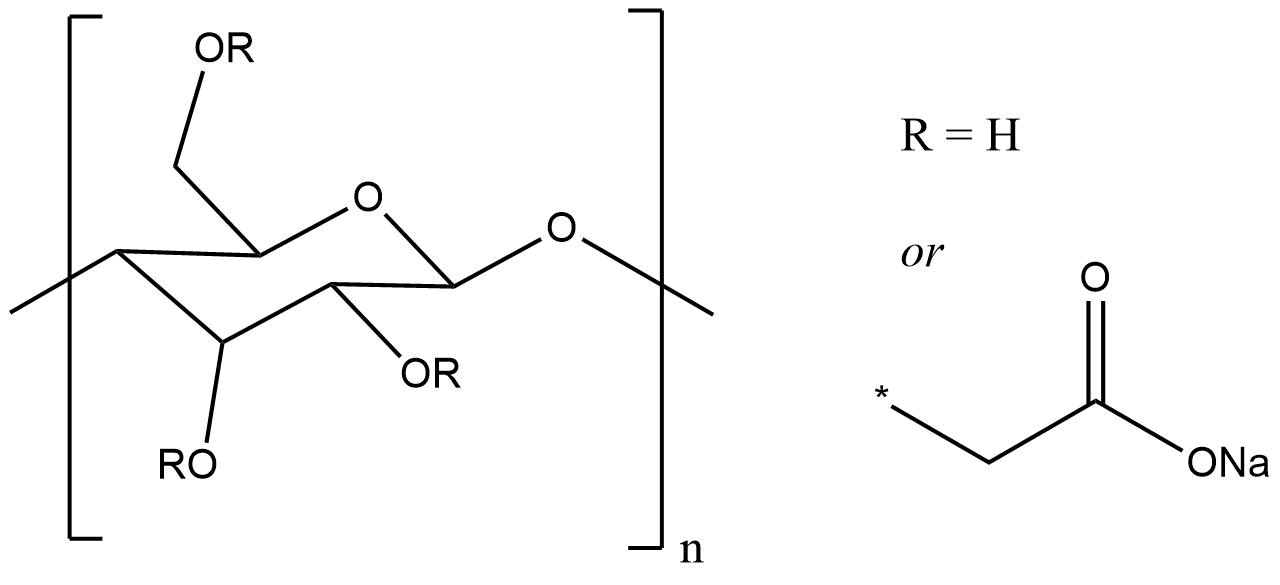
\includegraphics[width=0.8\columnwidth]{4-impregnation/figs/nc_structure.png}
    \caption{Structure of sodium carboxymethyl cellulose. \Acrfull{ds} is taken as the average number of sodium carboxymethyl groups (\ce{-CH2COONa}) per monomer.}
    \label{fig:nc_structure}
\end{figure}

Additionally, in chapter \ref{ch:impregnation} \acrfull{nc} was used as a precursor for direct (without \gls{htc}) activation. The structure of \acrshort{nc} is shown in figure \ref{fig:nc_structure}. Carbons were obtained from \acrshort{nc} with different \acrfullpl{ds} (\qtylist[list-final-separator={ or }, list-units=single]{0.0;0.7;0.9;1.2}), obtained from Sigma-Aldrich. For all samples, NC was heated under a flow of \ce{N2} (\qty{60}{\cm\cubed\per\minute}) at a rate of \qty{3}{\degreeCelsius\per\minute} and held for \qty{1}{\hour} at the target temperature of \qtylist[list-final-separator={ or }, list-units=single]{600;700;800}{\degreeCelsius}. Samples were washed in \qty{600}{\cm\cubed} of \qty{10}{\volpercent} \ce{HCl} solution, before being filtered and washed with deionised water to give neutral washings, and finally dried at \qty{100}{\degreeCelsius} for \qty{24}{\hour}. Samples are designated as NC\textit{x.x-TTT} where \acrshort{nc} indicates sodium carboxymethyl cellulose, \textit{x.x} is the \acrshort{ds}, and \textit{TTT} is the activation temperature. 

\section{Composition and morphology}
Techniques in this section were employed to understand the composition, structure, and porosity of samples synthesised in this work, and their results are presented in chapters \ref{ch:cbs} and \ref{ch:impregnation}. The more precise compositional analysis techniques - \acrfull{xps} and \acrfull{icp-oes} - as well as electron microscopy were only used for samples produced from \acrfullpl{ucb} in chapter \ref{ch:cbs}.

\acrfull{tga} measures the mass of a sample undergoing heating as a function of temperature or time.\citep{coats1963thermogravimetric} \acrshort{tga} was used in this study primarily to determine the \gls{ash content} of samples, thus giving a measure of sample purity,\citep{mcnaught1997compendium} i.e. whether the material contains any non-combustible matter, typically residual metals. For this work, \acrshort{tga} was performed using a TA Q500 Thermogravimetric Analyser. All samples were analysed using a platinum pan under a flow of air at \qty{100}{\cm\cubed\per\min}. All experiments took place as follows; temperature was increased at \qty{10}{\degreeCelsius\per\minute} from ambient to \qty{1000}{\degreeCelsius} before dwelling for \qty{10}{\minute}.

CHN elemental microanalysis precisely determines the concentration (by weight) of carbon, nitrogen and hydrogen that make up a sample. This is achieved by total combustion of the sample at \qty{975}{\degreeCelsius} under pure oxygen. At this stage impurities such as sulfur, phosphorous, and halogen compounds are also removed \textit{via} various reactions. This results in a pure mixture of \ce{H2O}, \ce{CO2} and oxides of nitrogen, which is transferred by means of a flow of He to a reduction chamber where the nitrogen oxides are reduced to \ce{N2}. This mixture of three sample gases plus the He carrier gas is then equilibrated to precise and constant temperature, volume and pressure. \ce{H2O} and \ce{CO2} are then sequentially separated according to their thermal conductivity, leaving a flow of \ce{N2} and \ce{He}. The volumes of \ce{H2O} and \ce{CO2} can then directly be used to calculate the sample \ce{H} and \ce{C} concentrations. The mixture of \ce{N2} and \ce{He} is compared with a reference flow of pure \ce{He} to determine \ce{N} content. For this study, CHN analysis was performed using an Exeter Analytical CE-440 Elemental Analyzer.
% find citation
% particular details of machine.

In general \acrfull{p-xrd} is principally used to identify elements and determine inter-layer spacing within crystalline powder samples. In the case of the partially-ordered \glspl{turbostratic carbon} and \glspl{hydrochar} reported in this thesis \acrshort{p-xrd} was used to determine the extent of graphiticity (i.e. how ordered the turbostratic domains are). In addition sharp peaks indicate the presence of crystalline material, which can be attributed to contaminants - typically residual \gls{porogen}. In this study, \acrshort{p-xrd} measurements were made using a PANalytical X’Pet Pro diffractometer, with \ce{Cu}K\textgreek{α} X-rays of wavelength \qty{1.54}{\angstrom}. Data collection occurred at 2\textgreek{θ} from \qtyrange[range-units=single]{2}{80}{\degree}.

X-ray photoelectron spectra are produced \textit{via} the irradiation of a sample with an X-ray beam, resulting in the ejection of electrons from low energy atomic orbitals according to the photoelectric effect\citep{richardson1912liii}. The electrons are collected and detected by the apparatus, facilitating the elucidation of the identity and quantity of elements present on the surface of the material from the kinetic energy of ejected electrons and the number of electrons ejected at each binding energy, respectively. The binding energy, $E_B$ is calculated according to the below equation;

\begin{equation}\label{eq:xps}
    E_B = h\nu - \Phi - E_K
\end{equation}

where $h\nu$ is the photon energy, $\Phi$ is the sample’s work function, and $E_K$ is the kinetic energy of the photoelectron. So-called `shifting' of elemental characteristic $E_B$ from those expected according equation \ref{eq:xps} can be used to determine chemical and electronic states of detected species.\citep{moulder1995handbook} For the purpose of \acrshort{xps} analysis in this work, samples were prepared from selected \glspl{hydrochar} and \glspl{turbostratic carbon} by performing a \acrshort{tga} in air to burn off all carbonaceous material. The remaining inorganic matter was then analysed using the Kratos AXIS ULTRA with a mono-chromated \ce{Al}k\textgreek{α} X-ray source (\qty{1486.6}{\electronvolt}) operated at \qty{10}{\mA} emission current and \qty{12}{\kilo\volt} anode potential (\qty{120}{\watt}). Spectra were acquired with the Kratos VISION II software. A charge neutralizer filament was used to prevent surface charging. Hybrid–slot mode was used measuring a sample area of approximately \qtyproduct{300 x 700}{\micro\metre}. The analysis chamber pressure was better than \qty{5e-9}{\milli\bar}. Three areas per sample were analysed. A wide scan at low resolution (Binding energy range \qtyrange{1400}{-5}{\electronvolt}, with pass energy \qty{80}{\electronvolt}, step \qty{0.5}{\electronvolt}, sweep time \qty{20}{\minute}) was used to estimate the total atomic \% of the detected elements. High resolution spectra at pass energy \qty{20}{\electronvolt}, step of \qty{0.1}{\electronvolt}, and sweep times of \qty{10}{\minute} each were also acquired for photoelectron peaks from the detected elements and these were used to model the chemical composition. The spectra were charge corrected to the C 1s peak set to \qty{285}{\electronvolt}. Casaxps (version 2.3.19 PR1.0) software\citep{fairley2021systematic} was used for quantification and spectral modelling.

Optical Emission Spectrometry (OES), also known as Atomic Emission Spectrometry (AES) is a technique used to quantify concentration of elements in solution by exciting them and measuring intensity of emissions at some characteristic wavelength associated with the return of the species to the ground state. These intensities are then converted to concentrations using a calibration curve. While there are multiple methods to excite the atoms, a common method is using Inductively Coupled Plasma (ICP) which also acts to separate elements in the solution. This technique is thus abbreviated to \acrshort{icp-oes} or ICP-AES.\citep{Hinners1988interlaboratory} In this work, samples were prepared for \acrshort{icp-oes} by dry-ashing in an alumina crucible at \qty{600}{\degreeCelsius} for at least \qty{16}{\hour}, the ash was then digested in an aqueous solution of \qty{10}{\volpercent} each of high purity \ce{HNO3} and \ce{HCl} (Aristar grade). The mixture was then sonicated for several hours, and digestion was completed via microwave, before being centrifuged at \qty{4000}{rpm} for \qty{99}{\minute}. Finally the digestate was filtered through syringe filters to remove any remaining sediment. References and blanks were prepared from the same stock digestion solution to ensure consistency. Standards were made from a 28-element standard (\qty{100}{\mg\per\dm\cubed}, \qty{2}{\volpercent} \ce{HNO3} matrix from Fisher) at concentrations of \qtylist[list-units = single]{0.1;1;10;50;100}{\mg\per\dm\cubed}. Measurements were made using a Perkin-Elmer Optima 2000 Spectrometer, using argon plasma.

\subsection{Electron microscopy}

Various forms of electron microscopy was used on the samples in chapter \ref{ch:cbs} in order to determine sample morphology as well as composition and dispersion of inorganic heteroatoms.

\paragraph{\acrfull{sem}} uses a beam of focused electrons in order to image solid materials. As the electrons interact with the material, electrons and electromagnetic radiation are emitted via various mechanisms. \Acrfull{se} are a result of the ejection of electrons from atoms near the sample surface, and \acrfull{sei} provide high resolution images of surface morphology and texture.\citep{Goldstein2017Scanning} 

\paragraph{\acrfull{bse}} are electrons deflected by nuclear electrostatic charge – degree of deflection increases with nuclear charge. Though this results in much lower resolution images, \acrfull{bed} images the material according to atomic weight, with heavier elements showing up as bright spots. This technique does not identify elements, but can be used to map heavier elements interspersed within a low atomic mass material.\citep{Goldstein2017Scanning}

\paragraph{\acrfull{tem}} differs from \acrshort{sem} in that the electrons are transmitted through the sample as opposed to reflecting off of it. Imaging with \acrshort{tem} allows for much more detailed imaging, down to the atomic scale.\citep{knoll1932elektronenmikroskop}

\paragraph{\acrfull{edx}} relies on the excitation by X-rays of electrons within a sample to identify and quantify its elemental components. It can be coupled with \acrshort{tem} in order to image the dispersion of elements within a sample, this technique is known as \acrshort{edx}-\acrshort{tem}.\citep{Goldstein2017Scanning}

\par \acrshort{sem} images were taken on a JEOL 7100F FEG-SEM with detector set at a working distance of 10.00 mm. SE images were captured with an electron accelerating voltage of 1.00 or 2.00 kV, but this was increased to 15.00 kV for BSE. %find TEM information

\section{Isotherms}\label{s:porosimetry}

In this work isotherms were measured in order to determine the porosity of the carbon samples as well as to find ambient temperature gravimetric \ce{CO2} uptake capacity as a function of pressure. The techniques used for these measurements are discussed below.

All \ce{N2} isotherms used for porosimetry were measured at \qty{-196}{\degreeCelsius} on a 3flex analyser from Micromeritics. Prior to isotherm measurement, all samples were degassed at \qty{300}{\degreeCelsius} for \qty{16}{\hour} under high vacuum. Adsorption were then measured in the relative pressure range \numrange{\sim e-8}{\sim1}, after which the desorption isotherm was measured down to \num{\sim0.1}. Thereafter free space was measured using \ce{He} at both ambient and analysis temperature and used to adjust the previously measured isotherm. From the isotherms, $A_{BET}$ values were determined using the Rouquerol method in the case of type-I isotherms,\citep{Rouquerol2007Is} otherwise this value was calculated using the linear portion of the BET transform within relative pressures between 0.05 and 0.30. Total pore volume ($V_t$) was determined from the volume adsorbed by the sample at a single point at relative pressure \num{\sim0.9} on the plateau of the isotherm. Classical determination of \gls{micropore} volume and surface area were determined using t-plot, with a carbon black STSA thickness curve. All \acrshortpl{psd} are derived using the 2D-NLDFT heterogeneous surface kernel in the SAIEUS software,\citep{Jagiello20132D} with the regularization parameter, $\lambda$\citep{Hansen1992Analysis, Hansen2001L} kept constant for samples derived from the same precursor and chosen to optimise fit across all isotherms. 

While the porosimetric analyses in chapters \ref{ch:cbs} and \ref{ch:impregnation} use only \ce{N2} isotherms, in chapters \ref{ch:dual_isotherm} and \ref{ch:pyPUC}  \ce{O2} and \ce{H2} isotherms measured at \qty{-196}{\degreeCelsius} were used to improve porosimetric analysis. \ce{O2} isotherms were measured in the same manner as for \ce{N2}, however \ce{H2} isotherms were measured up to  the arbitrary pressure of \qty{1013}{\milli\bar} as \ce{H2} is supercritical at \qty{-196}{\degreeCelsius} and thus relative pressure is not physically meaningful. In chapter \ref{ch:dual_isotherm}, the same classical measures of porosity were calculated from \ce{O2} isotherms as previously performed using \ce{N2} isotherms. In addition, comparisons were made of the \acrshortpl{psd} derived from fitting 2D-NLDFT heterogeneous surface kernels to \ce{O2}, \ce{N2}, and \ce{H2} isotherms. In addition, Jagiello's multiple isotherm fitting procedure\citep{Jagiello2015Dual} was employed with combinations of \ce{N2}, \ce{O2} and \ce{H2} isotherms to yield a single \acrshort{psd} for a single sample. These porosities derived from these alternative techniques were compared in \ref{ch:dual_isotherm}, and further used to assess the relationship between porosity and \ce{CO2} uptake in chapter \ref{ch:pyPUC}.

Excess \ce{CO2} uptake isotherms of \gls{turbostratic carbon} samples reported in chapters \ref{ch:cbs}, \ref{ch:dual_isotherm} and \ref{ch:pyPUC} was determined \textit{via} gravimetric analysis. This begins with the degassing of the samples under vacuum followed by precise measurement of the weight of the sample with increasing \ce{CO2} pressure. The procedure results in an excess \ce{CO2} uptake isotherm, from which molar gravimetric uptake can be read as a function of pressure. Measurements were taken at either \qtylist[list-pair-separator={ or }, list-units=single]{25;18}{\degreeCelsius} and up to \qtylist[list-pair-separator={ or }, list-units=single]{40;20}{\bar}, on XEMIS or IGA analysers respectively from Hiden Isochema. 

\section{Software development}
Chapter \ref{ch:pyPUC} describes the use of several python libraries in order to calculate linear regressions between porosity within some range of pore sizes to uptake of \ce{CO2} at some pressure. The main libraries used in this project, known as the python Porosity Uptake Correlator (pyPUC) are \verb|scipy|,\citep{SciPy2020} \verb|numpy|,\citep{numpy2022} \verb|pandas|,\citep{pandas2010} and \verb|pygaps|.\citep{Iacomi2019pyGAPS}

pyPUC is a fairly simple package whose structure is shown in figure \ref{fig:pyPUC_structure}. It is written almost exclusively in python,\citep{python1995} apart from one small bash script.\citep{bash2007} The main functions of pyPUC can be found in \verb|pyPUC/pyPUC/core|, while outside of this is the module \verb|pyPUC/interface.py| which constructs a simple command line interface to run the program, and the bash script \verb|pyPUC-cli| which executes \verb|pyPUC/interface.py|. Finally there is a directory for the \verb|source_data| which should be populated by the user with \acrshortpl{psd} and experimental uptake isotherms for the project in question.

\begin{figure}[ht!]
    \centering
    \begin{forest}
          for tree={
            font=\ttfamily,
            grow'=0,
            child anchor=west,
            parent anchor=south,
            anchor=west,
            calign=first,
            inner xsep=7pt,
            edge path={
              \noexpand\path [draw, \forestoption{edge}]
              (!u.south west) +(7.5pt,0) |- (.child anchor) pic {folder} \forestoption{edge label};
            },
            % style for your file node 
            file/.style={edge path={\noexpand\path [draw, \forestoption{edge}]
              (!u.south west) +(7.5pt,0) |- (.child anchor) \forestoption{edge label};},
              inner xsep=2pt,font=\small\ttfamily
                         },
            before typesetting nodes={
              if n=1
                {insert before={[,phantom]}}
                {}
            },
            fit=band,
            before computing xy={l=15pt},
          }  
        [pyPUC
          [pyPUC
            [core
              [best\_width\_at\_pressure.py,file]
              [psd\_processing.py,file]
              [uptake\_processing.py,file]
              [utils.py,file]
            ]
            [interface.py,file]
          ]
          [source\_data
            [project
              [psd
                [sorptive(s)]
              ]
              [uptake
                [sorptive]
              ]
            ]
          ]
          [pyPUC-cli,file]
        ]
    \end{forest}
    \caption{Structure of key modules and directories in the pyPUC package. There are other components in the github repository but they are not essential to the function of the package.}
    \label{fig:pyPUC_structure}
\end{figure}

The code is well documented, however a brief discussion of the purpose of each of the modules in \verb|pyPUC/pyPUC/core| follows here. Firstly \verb|utils.py| defines utility methods for the other three modules. Most important are the methods \verb|read_data()| and \verb|define_array()|. The former simply reads the data from the \verb|source_data| directory according to input arguments using the \verb|pandas| library,\citep{pandas2010} while the latter is a simple method for defining an array of pressures or pore widths for the modules \verb|uptake_processing| or \verb|psd_processing| using the \verb|numpy| library.\citep{numpy2022} 

\begin{table}[b!]
\centering
\captionof{table}{An example output of processed data from the \texttt{uptake\_processing.py} (a) and \texttt{psd\_processing.py} modules (b). \textit{A}, \textit{B}, \textit{C}, and \textit{D} are the four samples used in this analysis. In the case of (a), the numbers are the loadings of \ce{CO2} on the samples at each of the pressures in column \textit{p}, and for (b) they are the surface areas of the samples within the pore size range defined by $w_{min}$ and $w_{max}$.}
    \begin{subtable}{.5\linewidth}
      \centering
        \caption{}
        \begin{tabular}{l|l|l|l|l}
            p & A & B & C & D \\
            \midrule
            1 & 4.27 & 4.01 & 4.27 & 4.35 \\
            2 & 5.93 & 5.25 & 5.93 & 5.95 \\
            3 & 6.94 & 5.96 & 6.94 & 6.91 \\
        \end{tabular}
    \label{tb:loading_output}
    \end{subtable}%
    \begin{subtable}{.5\linewidth}
      \centering
        \caption{}
        \begin{tabular}{l|l|l|l|l|l}
            $\rm w_{min}$ & $\rm w_{max}$ & A & B & C & D \\
            \midrule
            5 & 4 & 59 & 282 & 238 & 260 \\
            6 & 4 & 401 & 514 & 442 & 465 \\
            6 & 5 & 142 & 232 & 204	& 204 \\
        \end{tabular}
    \label{tb:param_output}
    \end{subtable} 
\label{tb:loading_param_outputs}

\begin{python}
import pandas as pd
import numpy as np

sample_df = pd.read_csv('psd.csv')  # PSD stored in DataFrame 
w_array = [4, 5, 6]  # array of pore widths  
i=0
for wmax in w_array[1:]:  
    for wmin in w_array[w_array<wmax]:  # every possible combination of two w values
        rows_max = np.max(list(np.where(w < wmax)))
        rows_min = np.min(list(np.where(w > wmin)))
        max_value = sample_df.loc[rows_max, 'Vcum']
        min_value = sample_df.loc[rows_min, 'Vcum']
        param = max_value - min_value
        i+=1 # Go through all possible values of wmin for wmax
\end{python}
\captionof{figure}{How the porosity within some pore width range is determined in pyPUC. Note that this is pseudo-code\citep{davis2019pseudocode} as opposed to the actual source code.}
\label{fig:pypuc_porosity}
\end{table}

The \verb|uptake_processing.py| and \verb|psd_processing.py| modules are fairly self-explanatory, in each case simply processing the uptake or \acrshort{psd} data for all samples in \verb|source_data/project|. The outputs from these modules can be seen in figure \ref{tb:loading_param_outputs}. The former attempts to fit each uptake isotherm in the appropriate project in \verb|source_data| to a range of model isotherms and selects the best fit, by using the \verb|modelling| module from the library \verb|pygaps|.\citep{Iacomi2019pyGAPS} These model isotherms are then converted to point isotherms at pressures defined by the user. The pressures and loadings are then stored in a two-dimensional DataFrame, $D_\upsilon$ (see table \ref{tb:loading_output}). The latter reads in the cumulative \acrshortpl{psd} for each sample, and determines the pore volume or surface area within each user-defined pore size range. A demonstration of how this works is shown in figure \ref{fig:pypuc_porosity}. This is done for each sample and stored in the DataFrame $D_\pi$ (see table \ref{tb:param_output}). In either case, the data produced can be stored in memory or output as a \verb|.csv|, alongside a simple report of the data processing as shown in the appendix, figures \ref{fig:loading_report} and \ref{fig:psd_report}.

Finally \verb|best_width_at_pressure.py| takes the two DataFrames generated by \verb|uptake_processing.py| and \verb|psd_processing.py| and uses the \verb|stats.linregress()| method from the \verb|scipy| library\citep{SciPy2020} to perform linear regressions between each row of $D_\upsilon$ and each row of $D_\pi$. That is, if each of $D_\upsilon$ and $D_\pi$ have three rows (1, 2, 3) then a linear regression of row 1 in $D_\upsilon$ will be performed against each row 1, 2 and 3 of $D_\pi$. Then the same is performed for row 2 of $D_\upsilon$, etc.. \verb|scipy.stat.linregress()| then returns the $r^2$ value, slope, and intercept of the regression which is stored in the correlation DataFrame, $D_c$ alongside the values for $w_{min}$, $w_{max}$ and $P$ - an example of this can be seen in table \ref{tb:D_c}. $D_c$ can be reduced in size using the method \verb|correlation_requirements()| which allows rows in the DataFrame to be eliminated according to various arguments. The best pair of $w_{min}$ and $w_{max}$, according to the highest $r^2$ value for each pressure can be selected using the method \verb|make_correlation_df()|, i.e. yielding the optimum pore size region for uptake of the sorptive, $\Omega$.

\begin{table}[h!]
    \centering
    \begin{tabular}{l|l|l|l|l|l|l|l}
        $\rm w_{min}$ & $\rm w_{max}$ & p & $\rm r^2$ & m & c & x & y \\
        \midrule
        \rowcolor{yellow} 4 & 5 & 1 & 0.503 & -0.005 & 5.77 & [259 282 ...] & [4.27 4.01 ...] \\
        \rowcolor{yellow} 4 & 5 & 2 & 0.667 & -0.0157	& 9.85 & [259 282 ...] & [5.93 5.25 ...] \\
        4 & 5 & 3 & 0.691 & -0.0225 & 12.5 & [259 282 ...] & [6.94 5.96 ...] \\
        4 & 6 & 1 & 0.457 & -0.00213 & 5.20 & [401 514 ...] & [4.27 4.01 ...] \\
        4 &	6 & 2 & 0.662 & -0.00591 & 8.46	& [401 514 ...] & [5.93 5.25 ...] \\
        \rowcolor{yellow} 4 &	6 & 3 &	0.696 & -0.00854 & 10.5 & [401 514 ...] & [6.94 5.96 ...] \\
        5 & 6 & 1 & 0.254 & -0.00196 & 4.61 & [142 232 ...] & [4.27 4.01 ...] \\
        5 & 6 & 2 & 0.390 & -0.00561 & 6.86 & [142 232 ...] & [5.93 5.25 ...] \\
        5 & 6 & 3 & 0.413 & -0.00814 & 8.28 & [142 232 ...] & [6.94 5.96 ...] \\
    \end{tabular}
    \caption{Example output of a $D_c$ DataFrame from \ce{CO2} uptake and \acrshort{psd} data in table \ref{tb:loading_param_outputs}. Highlighted rows indicate the regression that yields the optimum pore size range ($\Omega$) for each of the pressures (1, 2, and 3 bar). Columns x and y indicate the surface area and loadings used for the regression, respectively. Values are truncated to save space.}
    \label{tb:D_c}
\end{table}
\bibliographystyle{rsc}
\bibliography{bibliography/bib}

%\chapter{Turbostratic carbons from ligno-cellulosic biomass}
\label{ch:syntheses}

\newpage

\section{Introduction}

\section{Precursor selection, synthesis \& sample designation}

\section{Results \& Discussion}
\subsection{Cigarette Butts}
\label{ss:cigarette_butts}


\subsubsection{Sample composition}
A primary goal of synthesising the carbons from cigarette butts was quantification and identification of so-called contaminant-porogens in cigarette butts, and monitoring their presence upon conversion of cigarette butts to hydrochar then to turbostratic carbon. Initial identification and rough quantification of the contaminants was performed using P-XRD and TGA respectively, with reference to CHN elemental microanalysis. Attempts were made to identify and more precisely quantify components using XPS and ICP-OES. Finally, imaging of the dispersion of contaminant-metals within unwashed turbostratic carbons was performed using BSE-SEM and EDX-TEM.

\paragraph{Cigarette Butts}

\paragraph{Hydrochars}
In the case of samples in sets \textit{hC} and \textit{hD} 

\paragraph{Activated Carbons}

\subsubsection{Porosity}

\subsubsection{\ce{CO2} uptake}

\subsection{Sawdust}
\label{ss:sawdust}

\subsection{Sodium Carboxymethyl Cellulose}
\label{ss:nc}

\subsubsection{Composition}

\subsubsection{Porosity}

\paragraph{Hysteresis}

\subsubsection{\ce{CO2} uptake}

\section{Conclusions}

\section*{References}
\chapter{Turbostratic carbons I: from cigarette butts}
\label{ch:cbs}

\newpage
\section*{Abstract}

Sequential \gls{htc} and KOH-mediated activation of \acrfullpl{ucf} has previously been shown by the author to provide a solution to the problem of \acrfull{cb} waste, in the form of an extremely promising \ce{H2} storage medium (see \ref{pub:CB}). The following study serves to expand the previous work \textit{via} carbonisation of \gls{hydrochar} derived from whole \acrfullpl{ucb} i.e. including the wrapping paper. \ce{KOH} activation of \acrshort{ucb}-\gls{hydrochar} yields carbons with much lower porosity than in \ref{pub:CB}, achieving micro-mesoporous carbons with $A_{BET}$ of up to \qty{1875}{\metre\squared\per\gram} and pore volume of \qty{0.89}{\cm\cubed\per\gram} at an activation temperature of \qty{700}{\degreeCelsius}. Thus, these materials are best applied to room temperature \ce{CO2} capture, with reasonable uptakes of \num{2.7} and \qty{14.1}{\milli\mole\per\gram} achieved at 1 and \qty{20}{\bar}, respectively.

\acrshortpl{ucb} are an unusual carbon precursor in that they contain a relatively high quantity, and diverse range of metals. As a result the composition and elemental distribution in \acrshortpl{ucb}, as well as in derived \glspl{hydrochar} and \glspl{turbostratic carbon} is investigated, as well as the efficacy of post-synthetic washing steps. \acrshortpl{ucb} and derived, unwashed \gls{hydrochar} were found to contain \ce{Al}, \ce{Fe}, \ce{K}, \ce{Mg}, \ce{Na}, \ce{Ti}, and \ce{Ca} in concentrations above \qty{0.10}{\mg\per\gram}. Many of these elements were also identified in derived \glspl{turbostratic carbon}. While it was hypothesised in \ref{pub:CB} that such contaminants may have an activating effect, there is no evidence of this in this work. Indeed, the stubbornness of these elements to removal \textit{via} \ce{HCl} washing results in porosity that is lower than expected indicating that these contaminants are limiting pore accessibility.

\newpage
\section{Introduction}

\acrfullpl{ucb} pose a large environmental hazard as a result of (i) being made of non-biodegradable \acrfull{ca} as well as (ii) containing a myriad of toxic chemicals.\citep{Slaughter2011, Puls2011, chevalier2018nano} As they are the most common waste material worldwide, there have been attempts to reduce their environmental presence, initially \textit{via} anti-littering campaigns.\citep{Prevention2011, Harris2011} More promising however is the prospect of valorising \acrshortpl{ucb} by various means, including conversion to activated carbons as reported by the author in \ref{pub:CB} as well as many other researchers.\citep{Soltani, Soltani2013, lima2018, xiong2019nitrogen, Lee2014, Hamzah2017, Yu2018, Wang2016a, Koochaki2019, Bilge2019}

\begin{figure}[h]
    \centering
    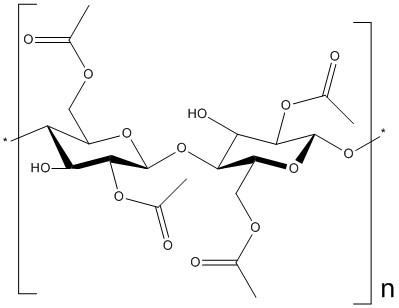
\includegraphics[width=0.7\columnwidth, keepaspectratio]{4-cbs/figs/cellulose_acetate.jpg}
    \caption{Structure of cellulose acetate.}
    \label{fig:cellulose acetate}
\end{figure}

\begin{sloppypar}
The reported porosity of carbons derived from \acrshortpl{ucb} is highly varied depending on synthetic conditions. In the absence of an \gls{activating agent}, and without pre-carbonisation steps, $A_{BET}$ typically does not exceed \qty{700}{\metre\squared\per\gram}.\citep{Koochaki2019, Soltani2013, Yazdi2012, Lee2014, Hamzah2017} Whereas using a \gls{porogen}, and/or pre-carbonising in air or hydothermally can improve surface areas to around \qty{3000}{\metre\squared\per\gram}.\citep{Xiong2018a, Koochaki2019, Sun2017, Bilge2019} The author's reports of ultrahigh porosity from KOH-activated hydrothermally carbonised \acrshortpl{ucb} in \ref{pub:CB} ($A_{BET}$ \qty{>4000}{\metre\squared\per\gram}, pore volume \qty{>2.00}{\cm\cubed\per\gram}) and high degree of microporosity (\qty{>90}{\percent}) are partially corroborated by the similar results using pure \acrfull{ca} in \ref{pub:CA}, suggesting that \acrshort{ca} is an ideal precursor for activation to yield high surface area carbons. Xiong \textit{et al.} also report a nitrogen-doped \acrshort{ucb}-derived activated carbon with hierarchical porosity and $A_{BET}$ of \qty{3420}{\metre\squared\per\gram}, though this result is dubious as (i) the \ce{N2} isotherm does not include ultralow pressure data, (ii) freespace appears to be incorrectly measured and (iii) isotherm measurement is not described in the text.\citep{xiong2019nitrogen} It was suggested in \ref{pub:CB} that the unusually high porosity of \acrshort{ucb}-derived carbons may be contributed to by the action of so-called contaminant-\glspl{porogen}, i.e. trace elements found in cigarette butts that can act as \glspl{activating agent} because carbons from \acrshortpl{ucb} had greater porosity than unused, i.e. `fresh' \acrshortpl{cb}. However, another factor may be the specific treatment of the \acrshortpl{ucb} prior to any carbonisation - that is the removal of any paper, residual ash and tobacco.
\end{sloppypar}

The trace element composition of \acrshortpl{ucb} have been studied by various means, including neutron activation analysis of the intact butts,\citep{iskander1992multielement, Iskander1985, jenkins1985neutron, Wu1997} \gls{adsorption} and emission spectroscopy of various aqueous extracts,\citep{MussaloRauhamaa1986, Kazi2009, Moriwaki2009, Moerman2011, Pelit2013, Dobaradaran2018} voltammetry experiments,\citep{Nitsch1991, Kalcher1993} as well as mixed methods according to environmental contaminant quantification standards.\citep{cardoso2018exposure} The reported concentration has a great degree of variability depending on collection site, method, and brand. For example, work by Iskander \textit{et al.} indicates that \ce{Al} can be present in concentrations as low as \num{59}, and as high as \qty{2200}{\micro\gram\per\gram}, depending on the country of origin of the smoked cigarette butt. Similarly, \acrshort{ucb} samples collected from the environment\citep{Dobaradaran2017, Moriwaki2009, Moerman2011, chevalier2018nano} may have lower quantities of some elements due to leaching, but simultaneously may absorb some elements from the environment (for example from sea water). Trace elements have been identified in \acrshortpl{ucb} from almost every region of the periodic table, including alkali and alkaline earth metals;\cite{MussaloRauhamaa1986, Iskander1985, iskander1992multielement, jenkins1985neutron, Wu1997, cardoso2018exposure}  transition metals, post transition metals and metalloids;\citep{MussaloRauhamaa1986, Dobaradaran2017, Iskander1985, jenkins1985neutron, Wu1997, Moriwaki2009, Moerman2011, Pelit2013, Dobaradaran2018, Ren2017, cardoso2018exposure, chevalier2018nano} lanthanides;\citep{iskander1992multielement} and halogens.\citep{Iskander1985, iskander1992multielement, jenkins1985neutron, Wu1997} Cigarette butt derived carbons have been also been found to contain various metals in trace quantities,\citep{Soltani, Soltani2013, Yazdi2012} although \ce{Ti}, \ce{K}, and \ce{Na} have also been reported at quantities above \qty{1}{\wtpercent}.\citep{Soltani, Soltani2013, Yazdi2012, lima2018, Lee2014} In addition the presence of \ce{Ca}, \ce{K}, \ce{Mg}, \ce{Na}, and \ce{Al} were identified in \acrshort{ucb}-derived \gls{hydrochar} reported in \ref{pub:CB}.

\begin{comment}
\begin{table}[b]
    \caption{Details of porosity and composition of selected \acrshort{ucb}-derived carbons.}
    \label{tb:cb_carbons_lit}
    \begin{tabularx}{\textwidth}{Xlllll}
        \toprule
            \textbf{Preparation} & \multicolumn{2}{c}{\textbf{Pyrolysis}} & $\mathbf{A_{BET}}\ /$ & \textbf{Elements} & \textbf{Ref.}\\ 
            & & & $\rm m^2\ g^{-1}$ &  &\\
            & $\mathbf{T\ /\ ^{\circ}C}$ & \textbf{\Gls{porogen}}  & & & \\
        \midrule
            & 900 & KOH (1) & 224 & K, Na, Si, Cl, Ti & \citep{Soltani} \\
            & 900 & - & 637 & Si, K, Ti & \citep{Yazdi2012} \\
            HTC & 190 & \ce{NaOH} (0.4) & - &  & \citep{lima2018} \\
            Add polypyrrole & 800 & KOH (1.5) & 3420 &  & \citep{xiong2018a} \\
            AC with NaOH & 800 & NaOH & 1083 & & \citep{Koochaki2019} \\
            & 800 &  & 571 & & \citep{Koochaki2019} \\
        \bottomrule
    \end{tabularx}%
\end{table}
\end{comment}

\section[Synthesis]{Precursor selection, synthesis \& sample designation}
% may need to include more synthetic details depending on methodology section.

The genesis of this synthetic work is linked to results reported in \ref{pub:CB}, namely the unusually high surface area and microporosity found for samples derived from the KOH-activation of used cigarette filter derived \gls{hydrochar}. It was suggested in this report that this porosity was not solely a result of KOH but indeed that other \glspl{porogen} (so-called contaminant-\glspl{porogen}) may be present in the precursor. This made it important to (i) determine the identity of these  contaminant-\glspl{porogen}; (ii) test whether these high levels of (micro-) porosity could be attained using the whole cigarette butt; (iii) ascertain if the removal of these contaminant-\glspl{porogen} had an effect on porosity; and (iv) see if such contaminant-\glspl{porogen} do in fact confer porosity on their own. As a result, samples were synthesised both from public ash trays and from a single brand as well as with and without the wrapping paper. Full synthetic details can be found in table \ref{tb:cb_synthesis}. In all cases, \qty{2.5}{\gram} \acrshortpl{ucb} were ground in a spice grinder, hydrothermally carbonised with \qty{25}{\cm\cubed} water at \qty{250}{\degreeCelsius} (\qty{5}{\degreeCelsius\per\minute}), held \qty{2}{\hour} then activated for \qty{1}{\hour} with or without \ce{KOH}. After cooling, all samples were washed with \ce{HCl} for at least \qty{24}{\hour}, then filtered and washed with water to give neutral washings. Sample designation is h\textit{A-xTTT}, where \textit{A} is the sample prefix (see table \ref{tb:cb_synthesis}), \textit{x} is KOH:\acrshort{ucb} ratio (wt./wt.), and \textit{TTT} is activation temperature in \unit{\degreeCelsius}. A portion of each self activated (i.e. $x = 0$) sample in sets C and D was left unwashed to determine the efficacy of the final washing step. These are indicated with $'$, for example hC-0800$'$ indicates a sample activated at \qty{800}{\degreeCelsius} in the absence of \gls{activating agent}, which was not washed. To refer to the \gls{hydrochar} itself, the designation is h\textit{A}-hydrochar, e.g. \gls{hydrochar} derived from subset hD (see table \ref{tb:cb_synthesis}) is hD-hydrochar.

\begin{table}[t]
    \caption{Synthetic details of samples derived from cigarette butts.}
    \label{tb:cb_synthesis}
    \begin{tabularx}{\textwidth}{lXXl}
        \toprule
            \textbf{Prefix} & \textbf{Preparation} & \textbf{T / \unit{\degreeCelsius}} & \textbf{\# Samples} \\ 
        \midrule
            \textbf{hC}     & From public ash tray; Ash, excess tobacco removed before grinding. \Gls{hydrochar} washed with \qty{0.5}{\dm\cubed} water.              & \numlist[list-final-separator={, }]{600;700;800} & 9              \\
            \textbf{hD}     &  From public ash tray; Ash, excess tobacco removed before grinding.             & \numlist[list-final-separator={, }]{600;700;800} & 9             \\
            \textbf{hE}     & Single brand from single smoker. Paper, ash, excess tobacco removed before grinding              & \numlist[list-final-separator={, }]{600;700;800} & 3              \\
        \bottomrule
    \end{tabularx}%
\end{table}

\section{Results \& Discussion}
\label{s:cb_results}

% need comparison to other hydrochars and carbons
Yields of \glspl{hydrochar} and derived \glspl{turbostratic carbon} can be found in table \ref{tb:cb_yield} (refer to table \ref{tb:cb_synthesis} for syntheses of the three sets of carbons). The fact that the yield of hC-hydrochar is significantly less than that of hD-hydrochar indicates that washing the \gls{hydrochar} does remove some labile matter. Although hE-hydrochar was also not washed, it has a similar yield to hC-hydrochar perhaps indicating that the concentration of non-carbonisable material was lower in set E of cigarette butts. These differences in yield are also transferred to the overall yield (bracketed numbers) of derived \glspl{turbostratic carbon}, but not to the yield of the activation step considered on its own - indicating that whatever is removed by washing of the \gls{hydrochar} does not have a significant affect on the product of the pyrolysis step. It is noteworthy that the yields of washed and unwashed carbons (0\textit{TTT} and 0\textit{TTT}$'$, respectively) are very similar, indicating that the extensive post-pyrolysis washing step does not remove significant amounts of material. Yields of \ce{KOH}-activated samples are of course significantly lower than samples pyrolysed in the absence of external \gls{activating agent}, due to removal of \ce{C} \textit{via} the dissolution of \ce{K2CO3} from the carbon framework during washing.

\begin{table}[t!]
    \caption{Average yields (\unit{\wtpercent}) of carbons derived from the three sets of used cigarette butt samples. The yield is taken as that of the single step in the synthesis; numbers in brackets are overall yield. Where cell is blank, this sample does not exist.}
    \label{tb:cb_yield}
    \begin{tabularx}{\textwidth}{llXlXlX}
        \toprule
            \textbf{xTTT} & \multicolumn{6}{c}{\textbf{Prefix}} \\
            & \multicolumn{2}{l}{\textbf{hC}} & \multicolumn{2}{l}{\textbf{hD}} & \multicolumn{2}{l}{\textbf{hE}} \\ 
        \midrule
            \textbf{hydrochar}  & 35 & & 50 & & 39 & \\
        \\
            \textbf{0600$'$} & 38 & (13) & 39 & (19) & & \\
            \textbf{0700$'$} & 35 & (12) & 33 & (17) & & \\
            \textbf{0800$'$} & 33 & (12) & 37 & (19) & & \\
        \\
            \textbf{0600} & 34 & (12) & 36 & (18) & 6 & (14) \\
            \textbf{0700} & 30 & (11) & 31 & (16) & 30 & (11)\\
            \textbf{0800} & 31 & (11) & 33 & (17) & 24 & (9)\\
        \\
            \textbf{4600} & 8 & (3) & 13 & (7) & & \\
            \textbf{4700} & 10 & (4) & 11 & (6) & & \\
            \textbf{4800} & 9 & (3) & 10 & (5) & & \\
        \bottomrule
    \end{tabularx}%
\end{table}


\subsection{Sample composition}

A primary goal of synthesising the carbons from cigarette butts was quantification and identification of so-called contaminant-\glspl{porogen} in \acrshortpl{ucb}, and monitoring their presence upon conversion of \acrshortpl{cb} to \gls{hydrochar} then to \gls{turbostratic carbon}. Initial identification and rough quantification of the contaminants was performed using \acrshort{p-xrd} and \acrshort{tga} respectively, with reference to CHN elemental microanalysis. Attempts were made to identify and more precisely quantify components using \acrshort{xps} and \acrshort{icp-oes}. Finally, imaging of the dispersion of contaminant-metals within unwashed \glspl{turbostratic carbon} was performed using \acrshort{bse}-\acrshort{sem} and \acrshort{edx}-\acrshort{tem}.

\begin{table}[t!]
    \caption{\ce{C}, \ce{H}, and \ce{N} content of \glspl{hydrochar} and carbons derived from cigarette butts, determined using elemental microanalysis as well as \gls{ash content} according to residual mass following TGA in air.}
    \label{tb:chn_ash}
    \begin{tabularx}{\textwidth}{lXXXX|X}
    \toprule
        & \multicolumn{4}{c}{\textbf{Contents / \unit{\wtpercent}}} \\
        \textbf{Sample} & \textbf{C} & \textbf{H} & \textbf{N} & \textbf{other} & \textbf{Ash} \\
    \midrule
        \textbf{hC-hydrochar} & 56 & 5 & 0 & 44 & 8 \\
        \textbf{hD-hydrochar} & 53 & 5 & 0 & 42 & 7 \\
        \textbf{hE-hydrochar} & 61 & 4 & 2 & 32 & \\
        &&&&&\\
        \textbf{hC-0600$'$} & 69 & 2 & 0 & 29 & 16 \\
        \textbf{hD-0600$'$} & 67 & 2 & 0 & 30 & 20 \\
        &&&&&\\
        \textbf{hC-0700$'$} & 71 & 1 & 1 & 27 & 19 \\
        \textbf{hD-0700$'$} & 72 & 0 & 0 & 27 & 13\\
        &&&&&\\
        \textbf{hC-0800$'$} & 77 & 0 & 0 & 22 & 18 \\
        \textbf{hD-0800$'$} & 77 & 0 & 0 & 21 & 12 \\
        &&&&&\\
        \textbf{hC-0600} & 68 & 2 & 0 & 30 & 20 \\
        \textbf{hD-0600} & 67 & 2 & 1 & 30 & 17 \\
        \textbf{hE-0600} & 77 & 2 & 2 & 19 & 2 \\
        &&&&&\\
        \textbf{hC-0700} & 71 & 1 & 1 & 27 & 14 \\
        \textbf{hD-0700} & 72 & 0 & 0 & 24 & 16 \\
        \textbf{hE-0700} & 81 & 2 & 2 & 16 & \\
        &&&&&\\
        \textbf{hC-0800} & 75 & 1 & 1 & 22 & 13 \\
        \textbf{hD-0800} & 77 & 0 & 0 & 22 & 20 \\
        \textbf{hE-0800} & 83 & 1 & 3 & 14 & 2 \\
        &&&&&\\
        \textbf{hC-4600} & 73 & 0 & 0 & 25 & 6 \\
        \textbf{hD-4600} & 58 & 0 & 0 & 41 & 31 \\
        &&&&&\\
        \textbf{hC-4700} & 78 & 0 & 0 & 22 & 5 \\
        \textbf{hD-4700} & 53 & 0 & 0 & 46 & 5 \\
        &&&&&\\
        \textbf{hC-4800} & 90 & 0 & 0 & 10 & 6 \\
        \textbf{hD-4800} & 50 & 0 & 0 & 50 & 37 \\
    \bottomrule
    \end{tabularx}
\end{table}
% find missing values
% Maybe repeat some TGA?

Relative proportions (by weight) of \ce{C}, \ce{H}, and \ce{N} for all \acrshort{ucb}-derived samples, as well as their \gls{ash content} can be found in table \ref{tb:chn_ash}. The composition of \glspl{hydrochar} and carbons activated without \ce{KOH} is essentially the same for samples in sets hC and hD. Furthermore the discrepancy in the \gls{ash content} of hC-hydrochar and hD-hydrochar is within margin for error. As such, it can be confirmed that the post-\gls{htc} washing step only serves to remove combustible matter, i.e. non-metals. The slightly larger discrepancies in \gls{ash content} between samples hC-0\textit{TTT} and hD-0\textit{TTT} (or hC-0\textit{TTT}$'$ and hD-0\textit{TTT}$'$) must therefore be ascribed to heterogeneous distribution of contaminants in the precursor, as opposed to removal of non-combustible contaminants prior to pyrolysis. Furthermore, washing of the \glspl{turbostratic carbon} does not seem to serve any consistent, significant role  in removing these contaminants. On the other hand, \ce{KOH}-activated samples (i.e. hC-4\textit{TTT} and hD-4\textit{TTT}) show more significant compositional differences, particularly in terms of \ce{C} content. This further confirms that the reduction in yield of hD-hydrochar relative to hC-hydrochar (see table \ref{tb:cb_yield}) is a result of removal of water-soluble organic material not incorporated into the \gls{hydrochar} macrostructure; it appears that the \ce{KOH} destroys such material in hD-4\textit{TTT}, thus reducing \ce{C} content. The higher \ce{C} and lower \gls{ash content} of hE-hydrochar and hE-0\textit{TTT} samples is an indication that the majority of the non-combustible contaminants seen in the ash of hC and hD samples come from the \acrshort{ucb} wrapping paper as opposed to the \acrshort{ucb} itself. In fact, the \gls{ash content} is zero (within margins for error) for the hE samples, and as a result the composition of these samples is much easier to discern; the `other' column simply represents the \ce{O} content. Unsurprisingly \ce{C} content increases, and \ce{O} content decreases with increasing activation temperature as consistently reported elsewhere.\citep{Blankenship2022Modulating, Sevilla2014Energy}

\begin{table}[b!]
    \caption{Gravimetric concentrations of metals in \acrshort{ucb} (including paper), wrapping paper and its derived, unwashed hydrochar according to ICP-OES. Samples derived from same batch of \acrshort{ucb} as used to make hC and hD samples - see table \ref{tb:cb_synthesis}}
    \label{tb:icp}
    \begin{tabularx}{\textwidth}{lXXXX}
    \toprule
         \multicolumn{2}{l}{\textbf{Analyte} ($\lambda$ / \unit{\nano\metre})} & \multicolumn{3}{c}{\textbf{Concentration / \unit{\mg\per\gram}}}\\
         & & \textbf{\acrshort{ucb}} & \textbf{\acrshort{ucb} paper} & \textbf{hydrochar}\\
    \midrule
        \textbf{\ce{Al}} & (396.153) & 1.58 & 46.0 & 4.81  \\
        \textbf{\ce{Fe}} & (283.204) & 2.81 & 38.6 & 3.66  \\
        \textbf{\ce{K}} & (766.490) & 2.91 & 17.9 & 4.60 \\
        \textbf{\ce{Mg}} & (285.210) & 0.71 & 11.0 & 1.13 \\
        \textbf{\ce{Na}} & (589.590) & 0.27 & 6.25 & 0.73 \\
        \textbf{\ce{Ti}} & (334.940) & 1.07 & 8.75 & 0.87 \\
        \textbf{\ce{Ca}} & (317.933) & 13.1 & 283 & 17.2 \\
        \textbf{\ce{Zn}} & (213.857) & - & 0.50 & - \\
    \bottomrule
    \end{tabularx}
\end{table}

The presence of sharp peaks in \acrshort{p-xrd} spectra confirms the presence of crystalline material in most of the \gls{hydrochar} and \gls{turbostratic carbon} samples (see appendix, figures \ref{fig:xrd_hydrochar}-\ref{fig:xrd_KOH}). Due to the complexity of the spectra it is difficult to assign peaks to any particular specie. Therefore, \acrshort{xps} was used and identified \ce{Ti}, \ce{Na}, \ce{K}, and \ce{Ca} in dry-ashed \acrshortpl{ucb} (see appendix, figure \ref{fig:cb_xps}). although absolute concentrations are not determinable by this technique as (i) there are likely adventitious \ce{C} and \ce{O} atoms on the surface of the ash, and (ii) it is unlikely that all atomic species are accounted for. \acrshort{icp-oes} allowed more precise determinations of metals in \acrshortpl{ucb}, their wrapping paper, and a derived \gls{hydrochar} - results are shown in table \ref{tb:icp}. These results confirm the presence of metals identified in \acrshort{xps}, as well as identifying \ce{Al}, \ce{Fe}, and \ce{Mg} in all samples. \ce{Zn} was only found in quantifiable amounts for the \acrshort{ucb} wrapping paper. These metals have previously been identified in \acrshortpl{ucb} by Iskander and others.\citep{chevalier2018nano, cardoso2018exposure, iskander1992multielement, jenkins1985neutron} All trace elements were found to have a higher occurence in the paper as opposed to the whole \acrshort{ucb}. This may explain the much higher \gls{ash content} of \glspl{hydrochar} and \gls{turbostratic carbon} derived from whole \acrshortpl{ucb} as compared to unwrapped \acrshortpl{ucf}, i.e. hC/hD  samples versus those derived from hE and those reported in \ref{pub:CB} respectively. 

\subsubsection{Electron Microscopy}

Electron microscopy was used to determine the distribution of heavy elements within \glspl{hydrochar} and \glspl{turbostratic carbon}. Initially, comparison of BSE to SE was used to gain a rough measure of elemental distribution, and an example thereof is shown in figure \ref{fig:SEM_BSE}. In the case of \gls{hydrochar} samples (figure \ref{fig:SEM_BSE}(a, b)), there appears to be a random, continuous distribution of heavy elements throughout the sample. On the other hand, unwashed \glspl{turbostratic carbon} derived without the use of \ce{KOH} as \gls{porogen} (exemplified in figure \ref{fig:SEM_BSE}(c, d) by hD-0600$'$) show more distinct clusters of heavy elements, though the distribution is no less random. The lack of uniformity of heavy element distribution is unsurprising as these elements are unlikely to be distributed regularly in the \acrshort{ucb} precursor, and the hydrothermal and pyrolytic processes are unlikely to produce any more compositional homogeneity. 

\begin{figure}[ht!]
    \centering
    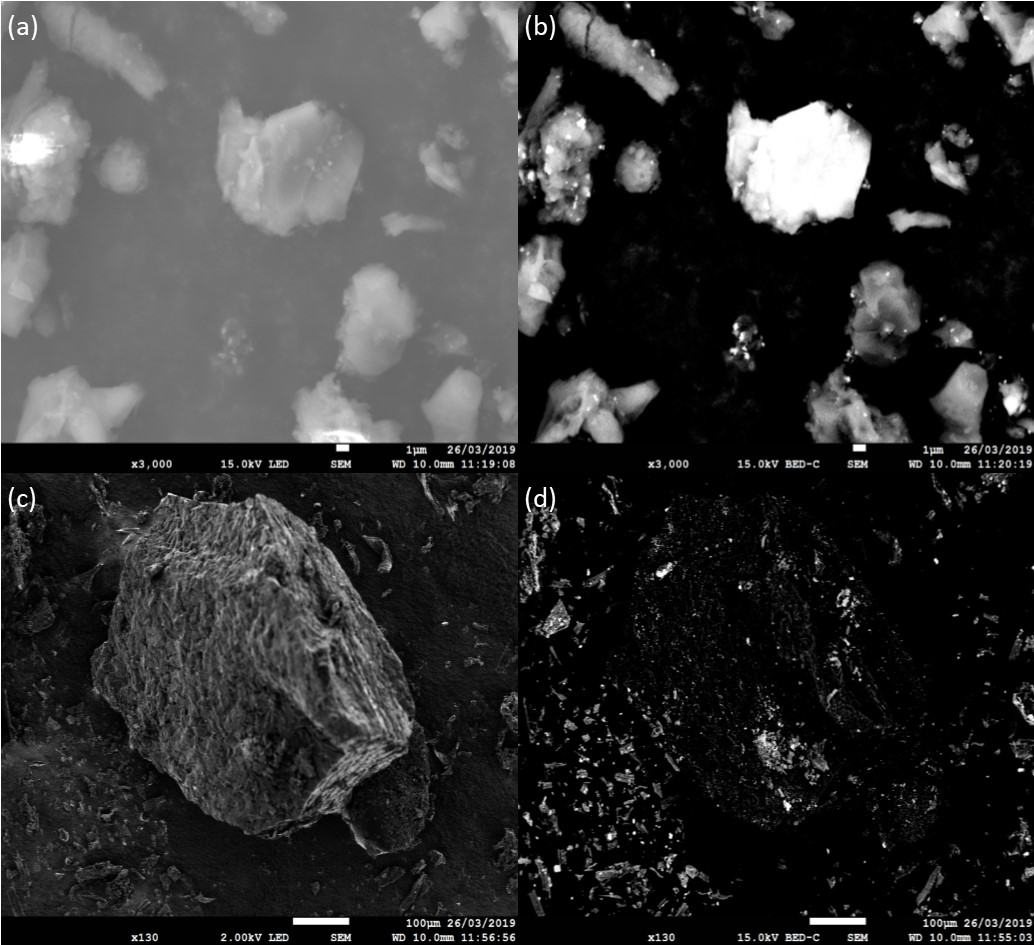
\includegraphics[width=\columnwidth, keepaspectratio]{4-cbs/figs/SEM_BSE.png}
    \caption{SE (a, c) and BSE (b, d) images of samples hD-hydrochar (a, b) and hD-0600$'$ (c, d).}
    \label{fig:SEM_BSE}
\end{figure}

\begin{figure}[b!]
    \centering
    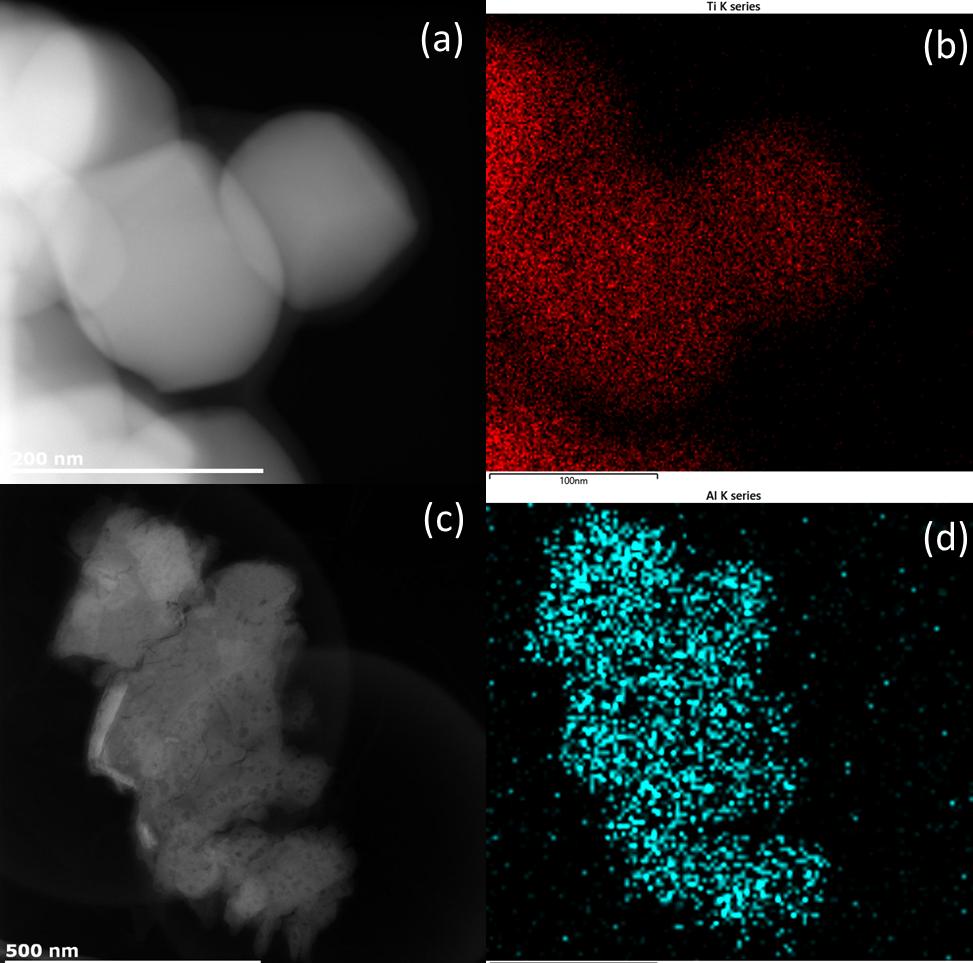
\includegraphics[width=\columnwidth, keepaspectratio]{4-cbs/figs/EDX_TEM.png}
    \caption{\acrshort{tem} (a, c) and \acrshort{edx}-\acrshort{tem} (b, d) images of hD-0700$'$ at sites 1 (a, b) and 3 (c, d). (b) and (d) show distribution of \ce{Ti} and \ce{Al} particles respectively.}
    \label{fig:EDX_TEM}
\end{figure}

For more detailed analysis of the distribution of elements in \glspl{turbostratic carbon}, EDX-TEM was used. Representative images derived using this technique are shown in figure \ref{fig:EDX_TEM}, and quantification at three different sites in table \ref{tb:cb_edx}. Most of the elements quantified by ICP-OES; \ce{Al}, \ce{Ca}, \ce{Cu}, \ce{K}, and \ce{Ti} are also identifiable by EDX-TEM, the \ce{Fe} and \ce{Na} are notably absent. In addition, \ce{Au} and \ce{Cr} are also present, though not in quantifiable amounts. The images in figure \ref{fig:EDX_TEM} show that heavy elements in the \glspl{turbostratic carbon} form clusters over the surface of the carbon structure. \ce{Ti} and \ce{Al} are the only metals whose concentrations were quantifiable at any site examined, with site 2 having \ce{Ti} as the majority component. \ce{Al} could only be quantified at site 3, wherein \ce{Ti} was notably absent in measurable quantities. Thus, it appears that at \ce{Ti} and \ce{Al} form discrete clusters within this \gls{turbostratic carbon}. On the other hand, the other metals identified by \acrshort{icp-oes} (see table \ref{tb:icp}) must be distributed more evenly meaning that they can not be as readily quantified in the small (roughly \qty{100}{\micro\metre\squared}) sites examined.

\begin{table}[t!]
    \caption{Concentrations of \ce{C}, \ce{O}, \ce{Al} and \ce{Ti} at three different sites in hD-4700 according to EDX-TEM }
    \label{tb:cb_edx}
    \begin{tabularx}{\textwidth}{llXlXlX}
    \toprule
        \textbf{Analyte} & \multicolumn{6}{c}{\textbf{Concentration / \unit{\wtpercent} (Atomic \unit{\percent})}} \\
        & \multicolumn{2}{l}{\textbf{Site 1}} & \multicolumn{2}{l}{\textbf{Site 2}} & \multicolumn{2}{l}{\textbf{Site 3}} \\
    \midrule
        \textbf{\ce{C}} & 80 & (90) & 33 & (36) & 73 & (82)\\
        \textbf{\ce{O}} & 8 & (7) & 4 & (5) & 14 & (12) \\
        \textbf{\ce{Al}} & - & (-) & - & (-) & 3 & (2) \\
        \textbf{\ce{Ti}} & 10 & (3) & 60 & (29) & - & (-) \\
    \bottomrule
    \end{tabularx}
\end{table}



\subsection{Porosity}

\begin{table}[hb!]
    \centering
    \caption{Porosity of \acrshort{ucb}-derived carbons from \ce{N2} isotherms. $A_{BET}$ determined using the Rouquerol method where applicable. Total pore volume, $V_t$ determined using the single point method. Numbers in brackets indicate micropore surface area and pore volume. Peak pore width, $w_{peak}$ (for samples hC-4\textit{TTT} and hD-4\textit{TTT}) taken as peak of the \acrshortpl{psd} in figure \ref{fig:cb_isopsd}.}
    \label{tb:cb_porosity}
    \begin{tabularx}{0.9\textwidth}{lllllll}
    \toprule
        \textbf{Sample} & \multicolumn{2}{l}{$\mathbf{A_{BET}}$ \textbf{/ \unit[detect-weight]{\metre\squared\per\gram}}}  & \multicolumn{2}{l}{$\mathbf{V_t}$ \textbf{/ \unit[detect-weight]{\cm\cubed\per\gram}}} & \multicolumn{2}{l}{$\mathbf{w_{peak}}$ \textbf{/ \unit{\angstrom}}} \\
    \midrule
        \textbf{hD-0600$'$} & 10 & (-) & - & (-) & \\
        \textbf{hD-0700$'$} & 170 & (150) & 0.07 & (0.06) \\
        \textbf{hD-0800$'$} & 226 & (198) & 0.09 & (0.08) \\
        & & & \\
        \textbf{hD-0600} & 120 & (104) & 0.05 & (0.04) & \\
        \textbf{hD-0700} & 122 &  (101) & 0.05 & (0.04) & \\
        \textbf{hD-0800} & 146 & (125) & 0.06 & (0.05) \\
        & & & \\
        \textbf{hC-4600} & 1428 & (1054) & 0.63 & (0.43) & 7  \\
        \textbf{hD-4600} & 1487 & (1036) & 0.64 & (0.41) & 7 \\
        & & & \\
        \textbf{hC-4700} & 1875 & (917) & 0.89 & (0.37) & 8 \\
        \textbf{hD-4700} & 1807 & (611) & 0.88 & (0.25) & 9  \\
        & & & \\
        \textbf{hC-4800} & 1958 & (626) & 1.00 & (0.26) & 8 \\
        \textbf{hD-4800} & 979 & (206) & 0.52 & (0.09) &  8 \\
    \bottomrule
    \end{tabularx}
\end{table}

As a result of the discovery of high quantities of non-combustible matter in turbostratic carbons which both were and were not washed, the effect of the washing step on porosity was examined. The results, i.e. porosity of samples hD-0\textit{TTT} and hD-0\textit{TTT}$'$ are shown in table \ref{tb:cb_porosity} alongside that for sets hC-4\textit{TTT} and hD-4\textit{TTT}. Isotherms and resultant PSDs for samples hC-4\textit{TTT} and hD-4\textit{TTT} are displayed in figure \ref{fig:cb_isopsd}.\footnote{Isotherms and PSDs for hD-0\textit{TTT} and hD-0\textit{TTT}$'$ can be found in the appendix, figure \ref{fig:0TTT_psdiso}, as well as full plots of isotherms and fits for all samples for which porosity is reported herein in figures \ref{fig:4TTT_psdisofull} and \ref{fig:0TTT_psdisofull}. Due to poor equilibration, the PSDs cannot be considered to be accurate. This issue is discussed in more depth in chapter \ref{ch:dual_isotherm} and \ref{pub:dual_iso}.}.  It is unclear whether washing in \ce{HCl} had any effect at all on porosity - indeed, for activation at 700 and \qty{800}{\degreeCelsius} there are significant reductions in $A_{BET}$ after washing. Perhaps this is simply a marker of physical agglomeration of particles during the washing process, and has little to do with internal porosity. Additionally, the porosity of these samples is not higher than would be expected for pyrolysed biomass; \gls{self-activation} of a pure cellulose acetate-derived \gls{hydrochar} yielded a carbon with $A_{BET}$  \qty{>500}{\metre\squared\per\gram},\footnote{Full porosimetric details of this sample are in appendix, figure \ref{fig:CA_psdiso} and table \ref{tb:CA_porosity}.} indeed \acrshort{ucb}-derived self-activated carbons have previously been shown to exhibit far higher surface areas.\citep{Soltani2013, Yazdi2012, Lee2014, Yu2018, Koochaki2019} As such there is no proof that the non-combustible contaminants can act as \glspl{porogen}. Of course this is not definitive as removal of contaminants proved impossible in these samples. The porosity that hD-0\textit{TTT} carbons \textit{do} possess is principally (over \qty{80}{\percent}, by surface area) in the \gls{micropore} region, though again this is to be expected for \glspl{biochar}/self-activated carbons.\citep{Weber2018Properties, Jagiello2019Enhanced, suliman2017role}

\begin{figure}[t]
    \centering
    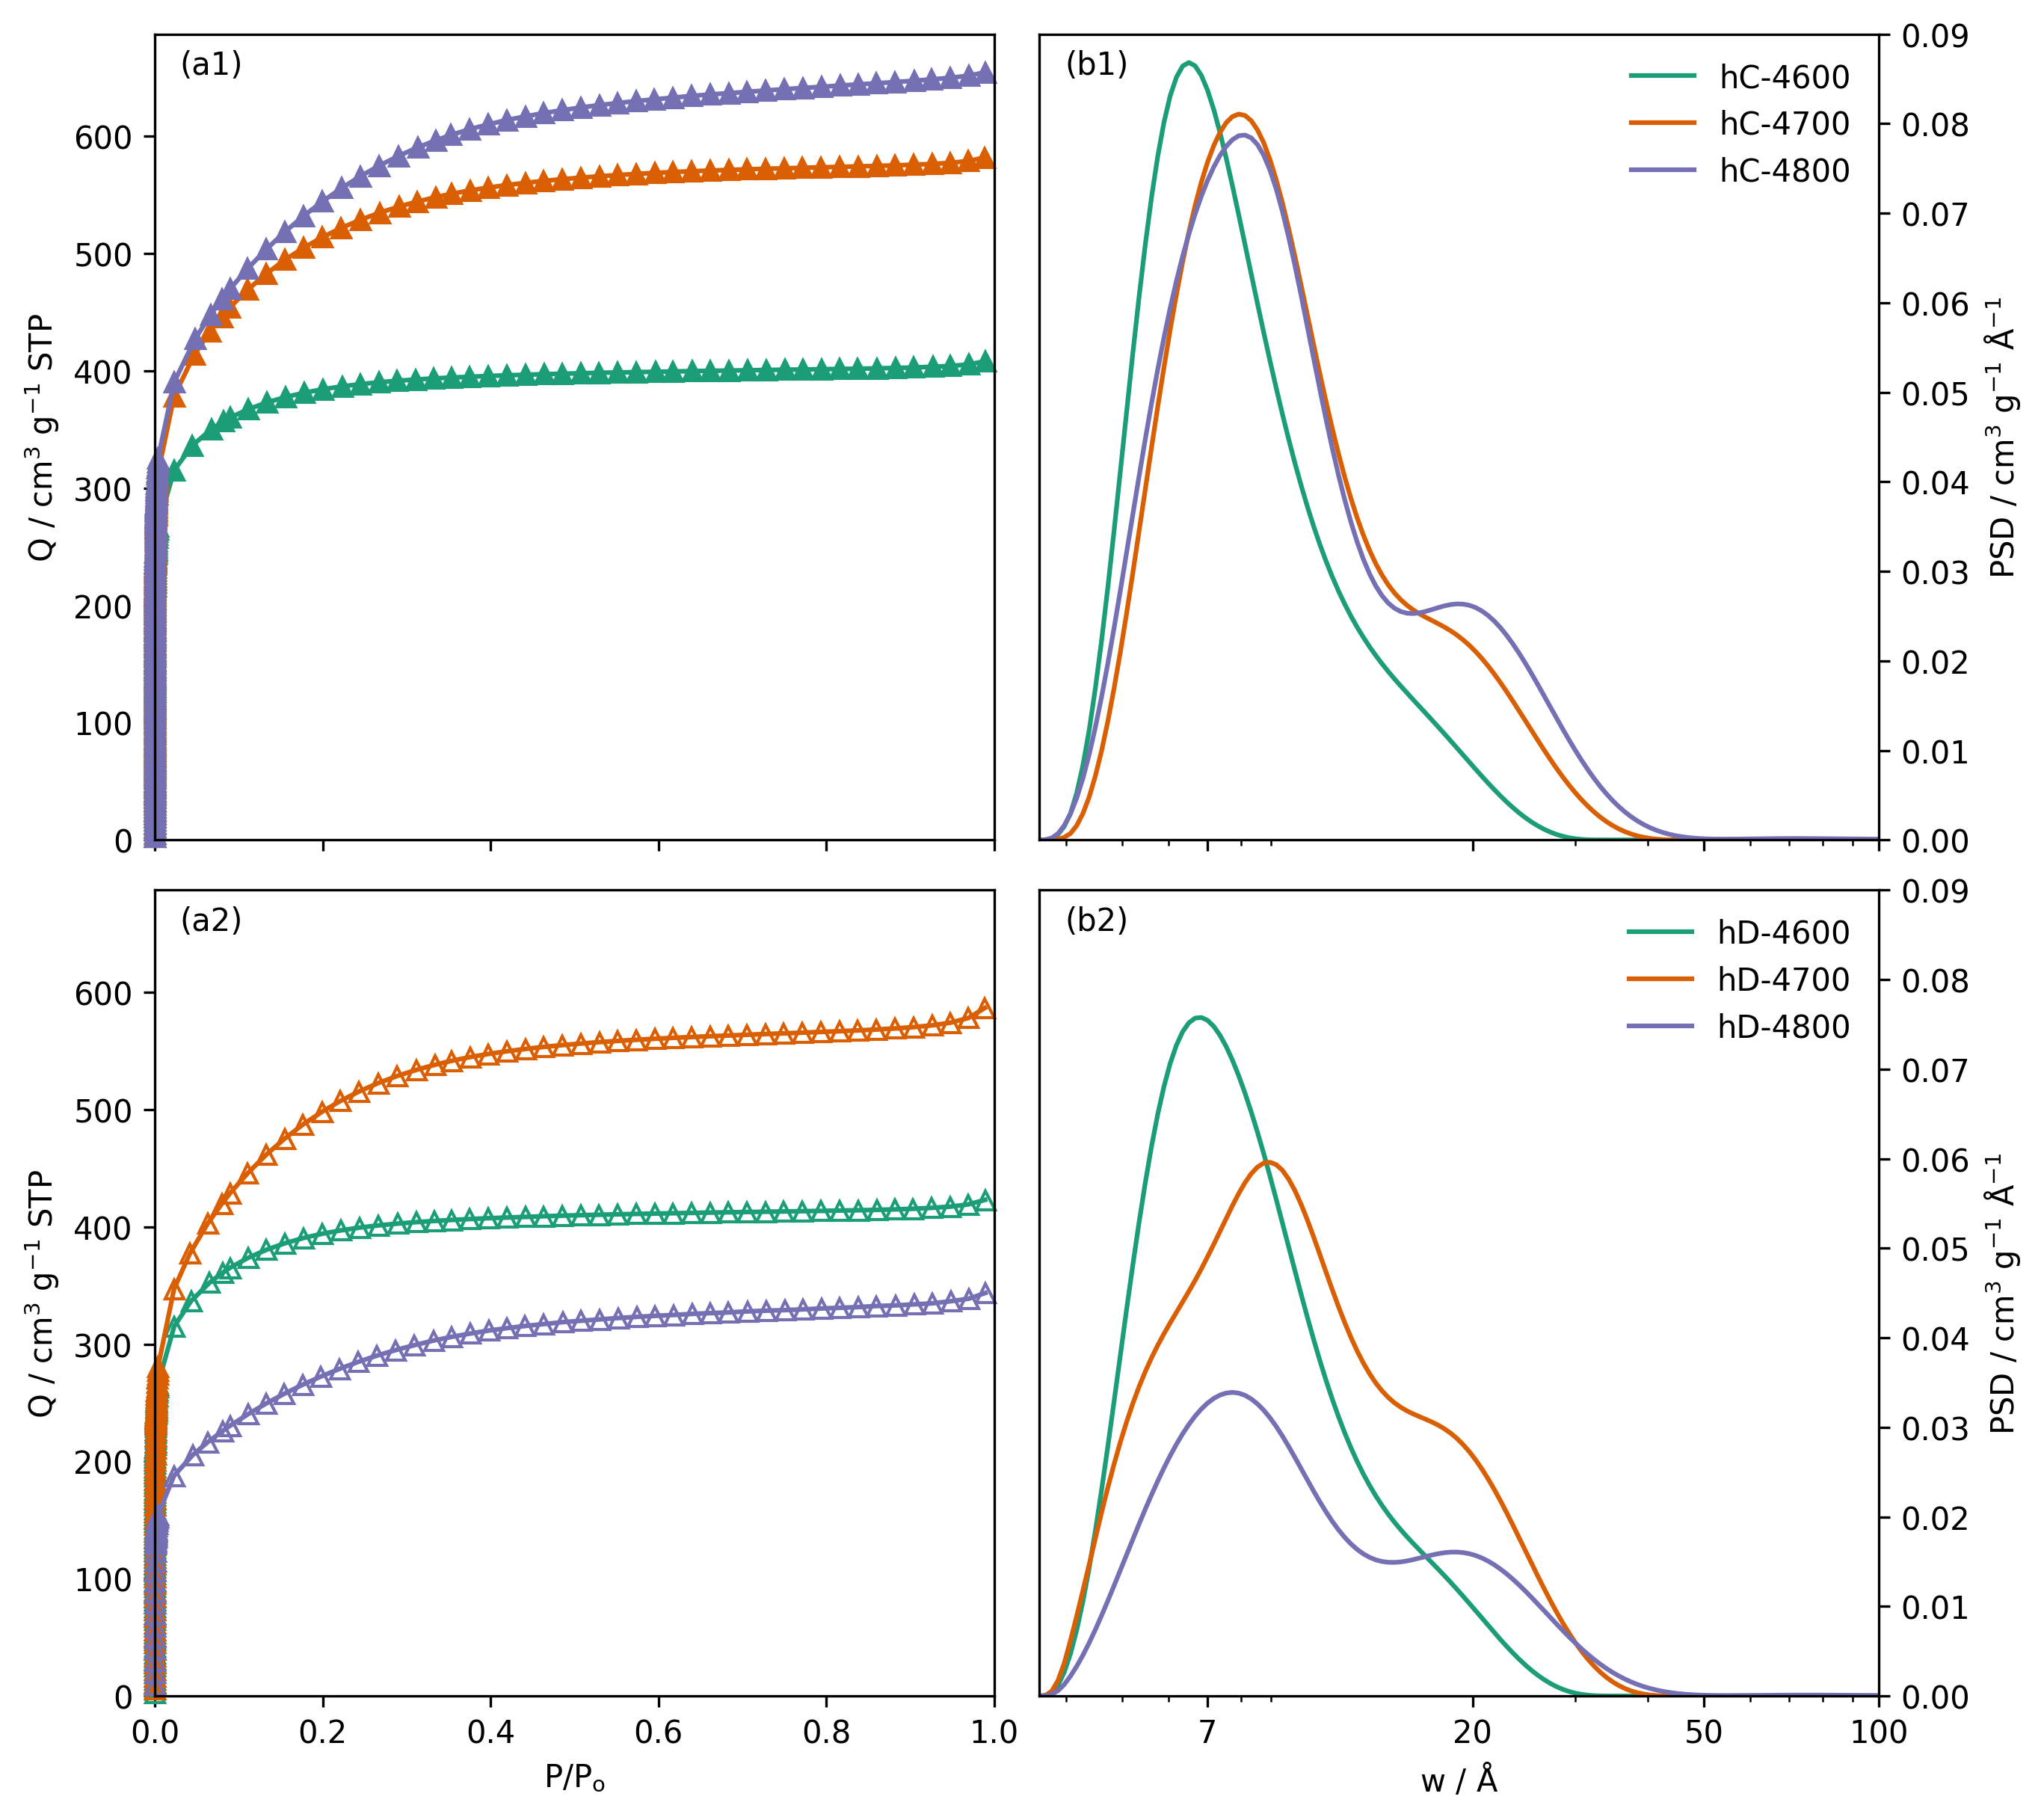
\includegraphics[width=\columnwidth, keepaspectratio]{4-cbs/figs/CB_n2_isotherms.png}
    \caption{Isotherms and resultant PSDs for samples hC-4\textit{TTT} and hD-4\textit{TTT}.}
    \label{fig:cb_isopsd}
\end{figure}

Carbons activated using \ce{KOH} have moderate surface areas, and a much lower relative microporosity than samples hD-0\textit{TTT}, ranging from \qty{71}{\percent} to as low as \qty{21}{\percent} when activated at \qtylist[list-units=single]{600;800}{\degreeCelsius} respectively. That is, these carbons are much more mesoporous, and mesoporosity increases with activation temperature. Indeed, the mesoporosity is reflected in the broad curvature of the \ce{N2} isotherms used to determine these textural characteristics as show in figure \ref{fig:cb_isopsd}(a1, a2). This is in contrast to the carbons reported in \ref{pub:CB}, where the author reported $A_{BET}$ of more than double that shown in this work, and all carbons were mostly microporous. This is likely a result of the relatively high (estimated) oxygen content, and thus low activation resistance (see \ref{pub:review}, \textbf{section 4.1.2.}) of the \glspl{hydrochar} formed in this work (see table \ref{tb:chn_ash}) as opposed to any limitations on porosity development resulting from the non-combustible contaminants. The lowest possible estimates of O-content for hC-hydrochar and hD-hydrochar are \qtylist[list-units=single]{37;35}{\wtpercent} respectively,\footnote{Minimum O-content taken as the difference between `other' and \gls{ash content} of the \glspl{hydrochar} (table \ref{tb:chn_ash}). The true value is likely much higher as the ash contains the oxides of non-combustible contaminants, thus weight reported is greater than in the carbon itself.} compared to \qty{25}{\wtpercent} for \acrshort{ucb}-derived \gls{hydrochar} in \ref{pub:CB}. 


Washing of the \gls{hydrochar} does not appear to have a consistent effect on porosity of derived KOH-activated carbons. That is,  $A_{BET}$ and pore volume are the essentially the same for both sets of carbons activated with \ce{KOH} at \qtylist[list-units=single]{600;700}{\degreeCelsius}, while porosity of hD-4800 is approximately half that of hC-4800. On the other hand, activation at \qtylist[list-final-separator={or }, list-units=single]{700;800}{\degreeCelsius} of unwashed \gls{hydrochar} results in much lower absolute microporosity relative to washed \gls{hydrochar}. This may be a result of combustion of volatile compounds dried into the unwashed \gls{hydrochar}, which produces oxidising gases such as \ce{CO} and \ce{CO2} leading to uncontrolled degradation of the carbon framework, and thus pore broadening.\citep{Sevilla2014Energy, Blankenship2022Modulating} This pore width broadening with increasing activation temperature is also evidenced by the PSDs of the carbons (see figure \ref{fig:cb_isopsd}(b1, b2)), with significantly more of the porosity above 20 \AA\space for samples activated at \qtylist[list-final-separator={or }, list-units=single]{700;800}{\degreeCelsius} relative to \qty{600}{\degreeCelsius}. The pores also become centered around higher values of $w$ (see table \ref{tb:cb_porosity}) with increasing activation temperature, though this trend is somewhat obscured for samples hD-4\textit{TTT} - but this may simply be an effect of reduction in overall porosity resulting from combustion of volatiles in the activation process. Pore size hierarchy does not appear to be significantly affected by the presence (or lack of) a \gls{hydrochar} washing step.

\subsection{\texorpdfstring{\ce{CO2} uptake}{CO2 uptake}}

While the ultra-high surface areas of carbons reported in \ref{pub:CB} made them excellent candidates for \ce{H2} storage, this is not the case for \acrshort{ucb}-derived KOH-activated carbons prepared in this work. The lower surface area and more hierarchical pore structure of these carbons (table \ref{tb:cb_porosity}) make them much better candidates for \ce{CO2} capture. As such, room temperature molar \ce{CO2} uptake was measured up to \qty{40}{\bar}, and results thereof are tabulated in table \ref{tb:cb_co2} and shown in full in figure \ref{fig:cb_co2}. 

\begin{table}[b!]
    \centering
    \caption{\ce{CO2} uptakes (measured at \qty{25}{\degreeCelsius}) at \qtylist[list-units=single]{1;20}{\bar} for samples hC-4\textit{TTT} and hD-4\textit{TTT}.}
    \label{tb:cb_co2}
    \begin{tabularx}{0.8\textwidth}{XXX}
    \toprule
        \textbf{Sample} & \multicolumn{2}{c}{\textbf{\ce{CO2} uptake / \unit[detect-weight]{\milli\mole\per\gram}}} \\
         & \textbf{1 \unit[detect-weight]{\bar}} & \textbf{20 \unit[detect-weight]{\bar}}\\
    \midrule
        \textbf{hC-4600} & 2.6 & 9.8 \\
        \textbf{hD-4600} & 1.5 & 6.1 \\
        \\
        \textbf{hC-4700} & 2.3 & 12.1 \\
        \textbf{hD-4700} & 2.3 & 14.1 \\
        \\
        \textbf{hC-4800} & 2.7 & 12.6 \\
        \textbf{hD-4800} & 1.5 & 9.7 \\
    \bottomrule
    \end{tabularx}
\end{table}

\begin{figure}[hb!]
    \centering
    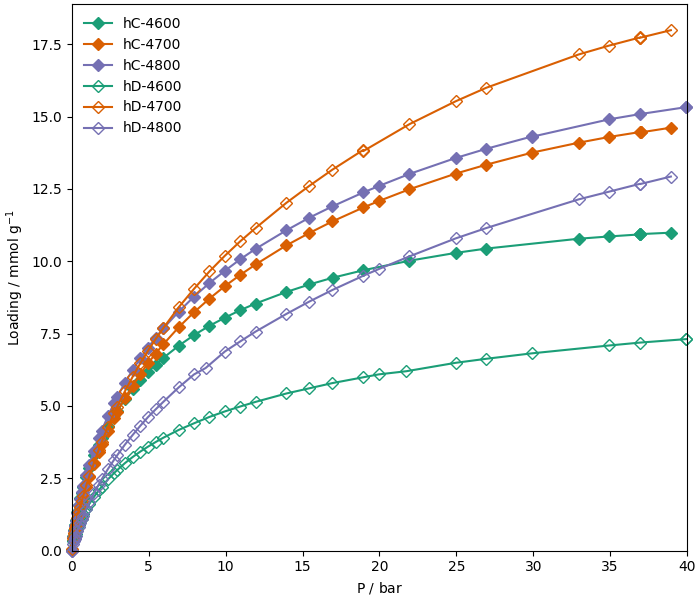
\includegraphics[width=\columnwidth, keepaspectratio]{4-cbs/figs/CB_CO2.png}
    \caption{\ce{CO2} uptake isotherms (298 K) for samples hC-4\textit{TTT} and hD-4\textit{TTT}.}
    \label{fig:cb_co2}
\end{figure}

At \qty{20}{\bar}, the highest surface area samples - hD-4700, hC-4700 and hC-4800 - perform the best as a result of maximisation of available adsorption sites for attractive London forces between \ce{CO2} and the material surface. The more mesoporous hD-4700 (see table \ref{tb:cb_porosity}) has a \qty{17}{\percent} greater \ce{CO2} uptake than the more microporous hC-4700 at \qty{20}{\bar}. This is likely because \glspl{mesopore} fill at higher pressure than \glspl{micropore}. Conversely, if we compare hC-4600 and hD-4600 the origin of the discrepancy in their \ce{CO2} uptake is unclear at both 1 and 20 bar, as their porosity is essentially identical. The only major distinction is compositional; hD-4600 has a far higher \gls{ash content} (see table \ref{tb:chn_ash}). Perhaps some contaminant prevents ingress of \ce{CO2} into hD-4600's pores. Optimum low pressure \ce{CO2} uptake is achieved by two samples with quite different porosity; hC-4600 and hC-4800. The high degree of microporosity ($A_{BET} = \qty{1023}{\metre\squared\per\gram}$, $V_t = \qty{0.64}{\cm\cubed\per\gram}$) in hC-4600 counteracts the greater overall porosity of hC-4800, whose pore volume is \qty{56}{\percent} greater than hC-4600. 

The \ce{CO2} uptakes of the two samples synthesised at \qty{600}{\degreeCelsius} approach a plateau at pressures in excess of \qty{10}{\bar}. This behaviour is likely a result of the fairly narrow \acrshortpl{psd} of these carbons. On the other hand, the slope of isotherms for the other four samples does not decrease to the same extent as they have a greater degree of hierarchy in their \acrshortpl{psd}. Thus the samples synthesised at \qtylist[list-units=single]{700;800}{\degreeCelsius} are more suitable for applications such as \acrshort{psa}.\citep{Sevilla2014Energy} The activation temperature-porosity-gas uptake capacity relationship is similar to that for carbons synthesised in \ref{pub:CA} and \ref{pub:CB}, in that optimum porosity for \ce{CO2} uptake is achieved at a lower than expected activation temperature of \qty{700}{\degreeCelsius}. In general in a series of \glspl{turbostratic carbon} derived through the activation of biomass, the optimum gas uptake is achieved for samples activated at \qty{\sim800}{\degreeCelsius}.\citep{Ariharan2018}

\section{Conclusion}

The KOH-mediated pyrolysis of whole \acrshortpl{ucb} does not yield carbons with ultrahigh porosity as shown in \ref{pub:CB}. This appears to be due to compositional differences, i.e. that the wrapping paper is not as readily activated as the \acrshort{ca} present in the filters themselves. As a result, KOH-activated materials do not show promise as \ce{H2} storage media, but instead their medium $A_{BET}$ (approaching \qty{2000}{\metre\squared\per\gram}) and hierarchical \acrshortpl{psd} make them useful for ambient temperature \ce{CO2} capture; \ce{CO2} uptakes of \qtylist[list-units=single]{2.7;14.1}{\milli\mole\per\gram} were achieved at \qtylist[list-units=single]{1;20}{\bar} respectively. 

Of further interest is the function of the two washing steps, i.e. after \gls{htc} and after pyrolysis. It appears that removal of non-combustible contaminants is inconsistent, although washing the \gls{hydrochar} \textit{does} remove volatile organic matter, which may slightly increase the concentration of \ce{C} in derived turbostratic carbons. On the other hand, washing of the carbons pyrolysed in the absence of KOH has inconsistent effects on porosity, and indeed on the concentration of non-combustible matter in the samples with \glspl{ash content} of up to \qty{20}{\wtpercent} even in washed carbons. In addition the porosity of these samples is lower than is found for carbon derived from the sequential \gls{htc} and pyrolysis of pure \acrshort{ca}, suggesting some interference of the stubborn metal contaminants with pore accessibility.

The difficulty in the removal of non-combustible contaminants led the author to investigate their nature. It was found through a combination of \acrshort{icp-oes}, \acrshort{xps}, and electron microscopy that \ce{Al}, \ce{Fe}, \ce{K}, \ce{Mg}, \ce{Na}, \ce{Ti}, and \ce{Ca} are present in whole \acrshortpl{ucb} and unwashed \gls{hydrochar}. In addition, nanoclusters of \ce{Au} and \ce{Cr} were also identified in an unwashed \gls{turbostratic carbon}. 

\bibliographystyle{rsc}
\bibliography{bibliography/bib}

%\newpage
\cleardoublepage
%\section*{Appendix}
%\label{cb:appendix}
%\addcontentsline{toc}{section}{\nameref{cb:appendix}}
%\appnums
\begin{subappendices}

\begin{figure}[h]
    \centering
    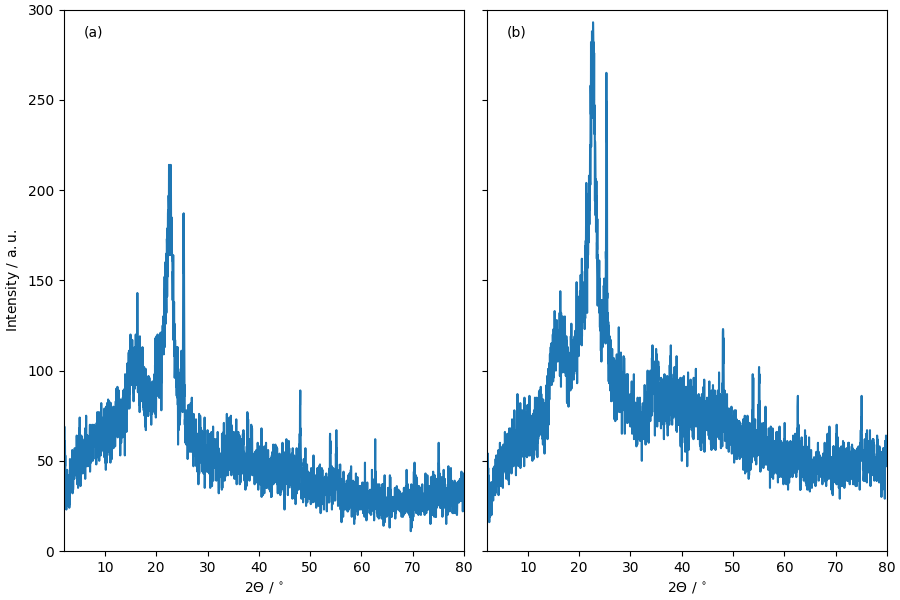
\includegraphics[width=\columnwidth, keepaspectratio]{4-cbs/figs/xrd_hydrochar.png}
    \caption{P-XRD spectra for samples hC-hydrochar (a) and hD-hydrochar (b).}
    \label{fig:xrd_hydrochar}
\end{figure}

\begin{figure}[h]
    \centering
    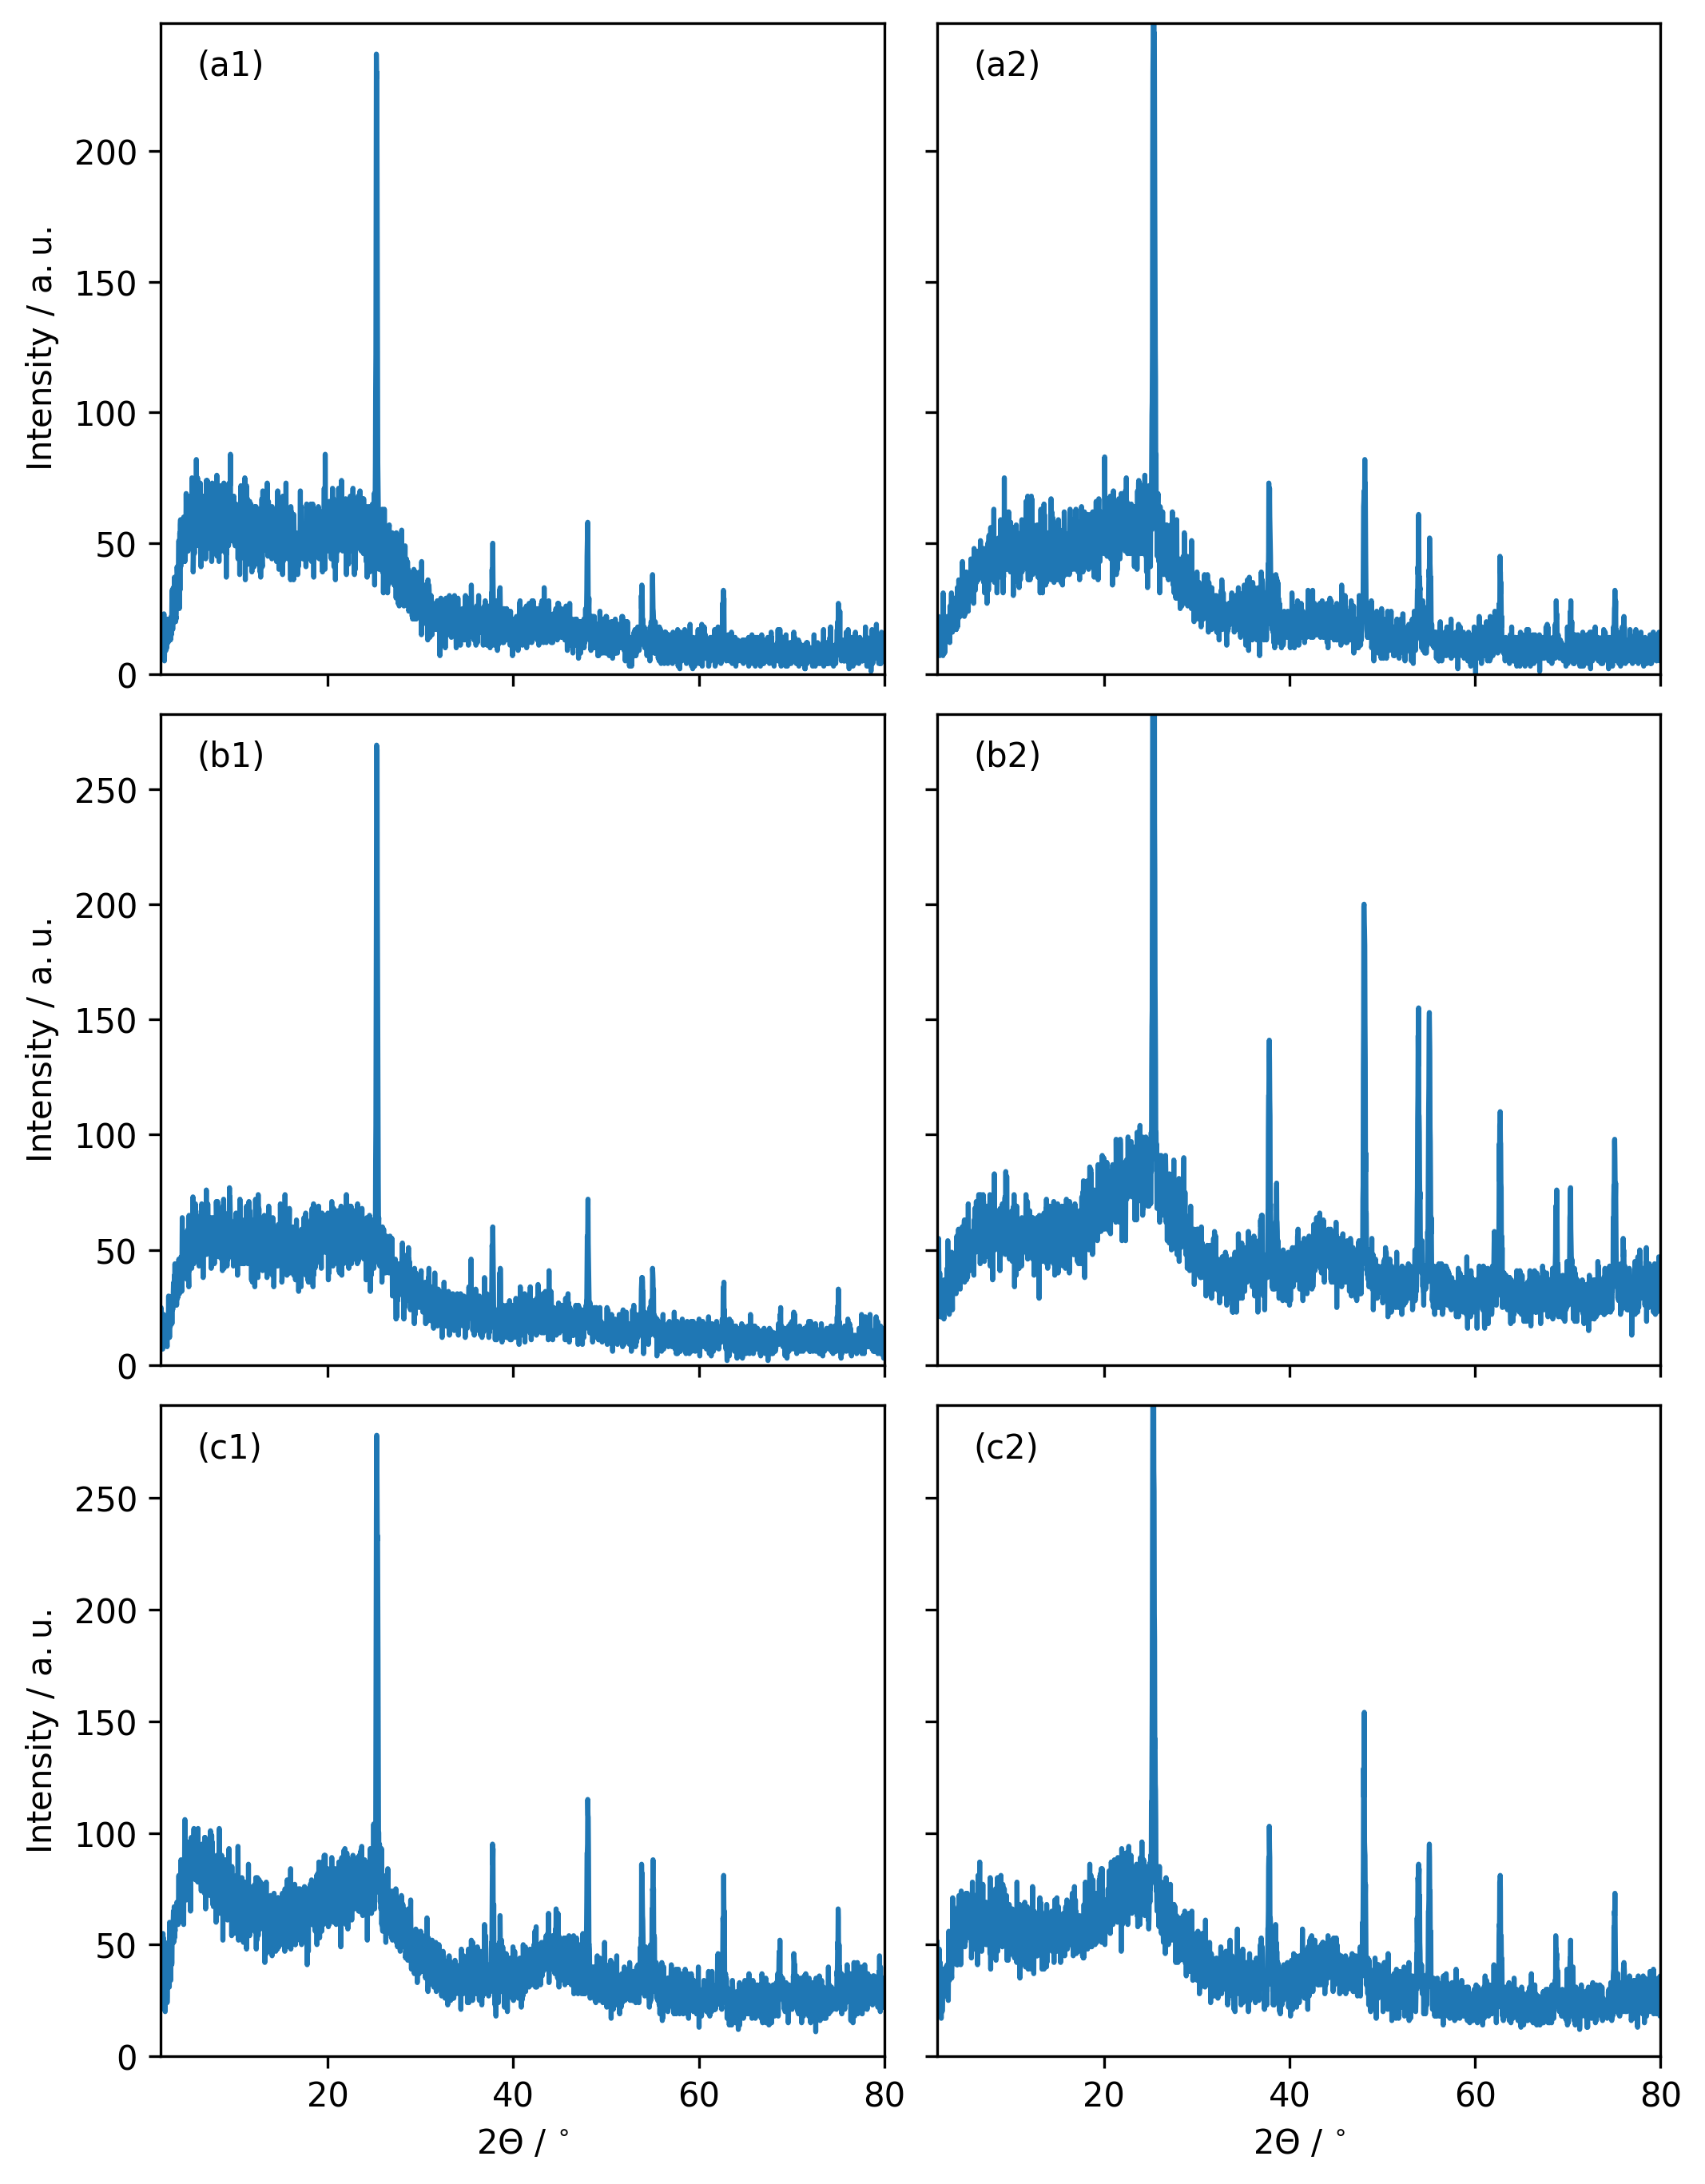
\includegraphics[width=\columnwidth, keepaspectratio]{4-cbs/figs/xrd_hC-0TTT.png}
    \caption{P-XRD spectra for samples hC-0600 (a1), hC-0600$'$ (a2), hC-0700 (b1), hC-0700$'$ (b2), hC-0800 (c1), hC-0800$'$ (c2).}
    \label{fig:xrd_hC-0TTT}
\end{figure}

\begin{figure}[h]
    \centering
    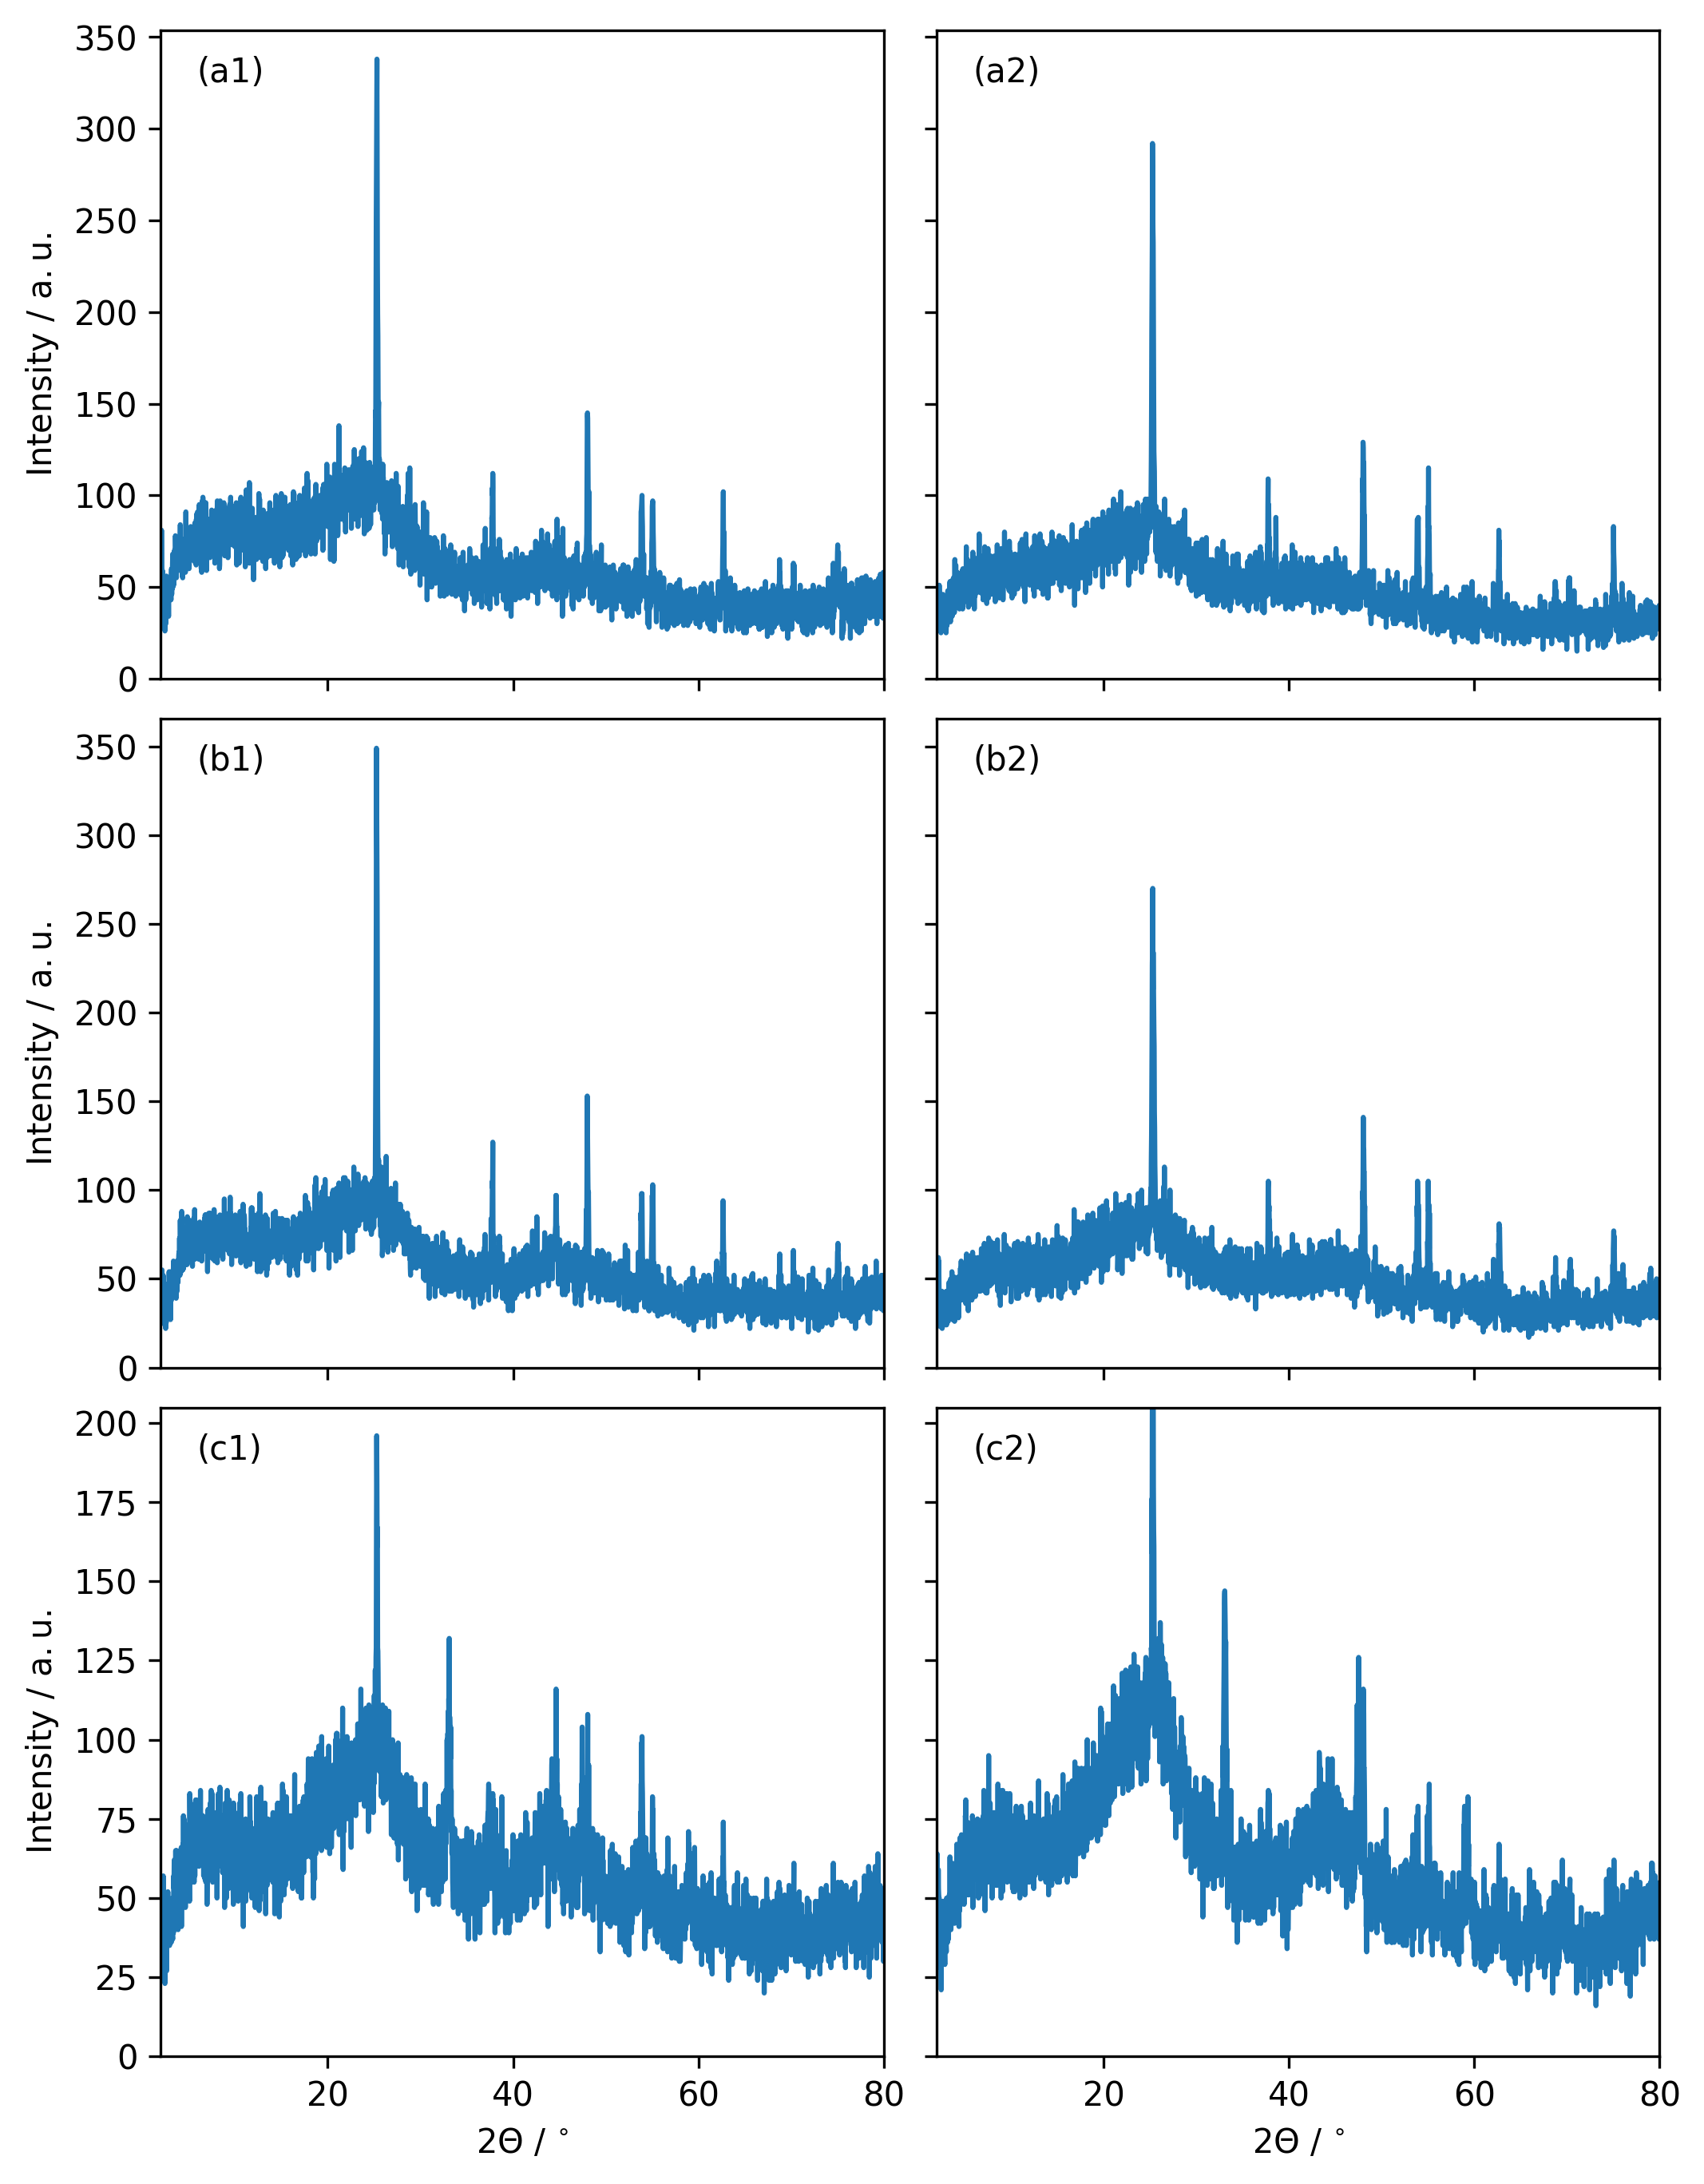
\includegraphics[width=\columnwidth, keepaspectratio]{4-cbs/figs/xrd_hD-0TTT.png}
    \caption{P-XRD spectra for samples hD-0600 (a1), hD-0600$'$ (a2), hD-0700 (b1), hD-0700$'$ (b2), hD-0800 (c1), hD-0800$'$ (c2).}
    \label{fig:xrd_hD-0TTT}
\end{figure}

\begin{figure}[h]
    \centering
    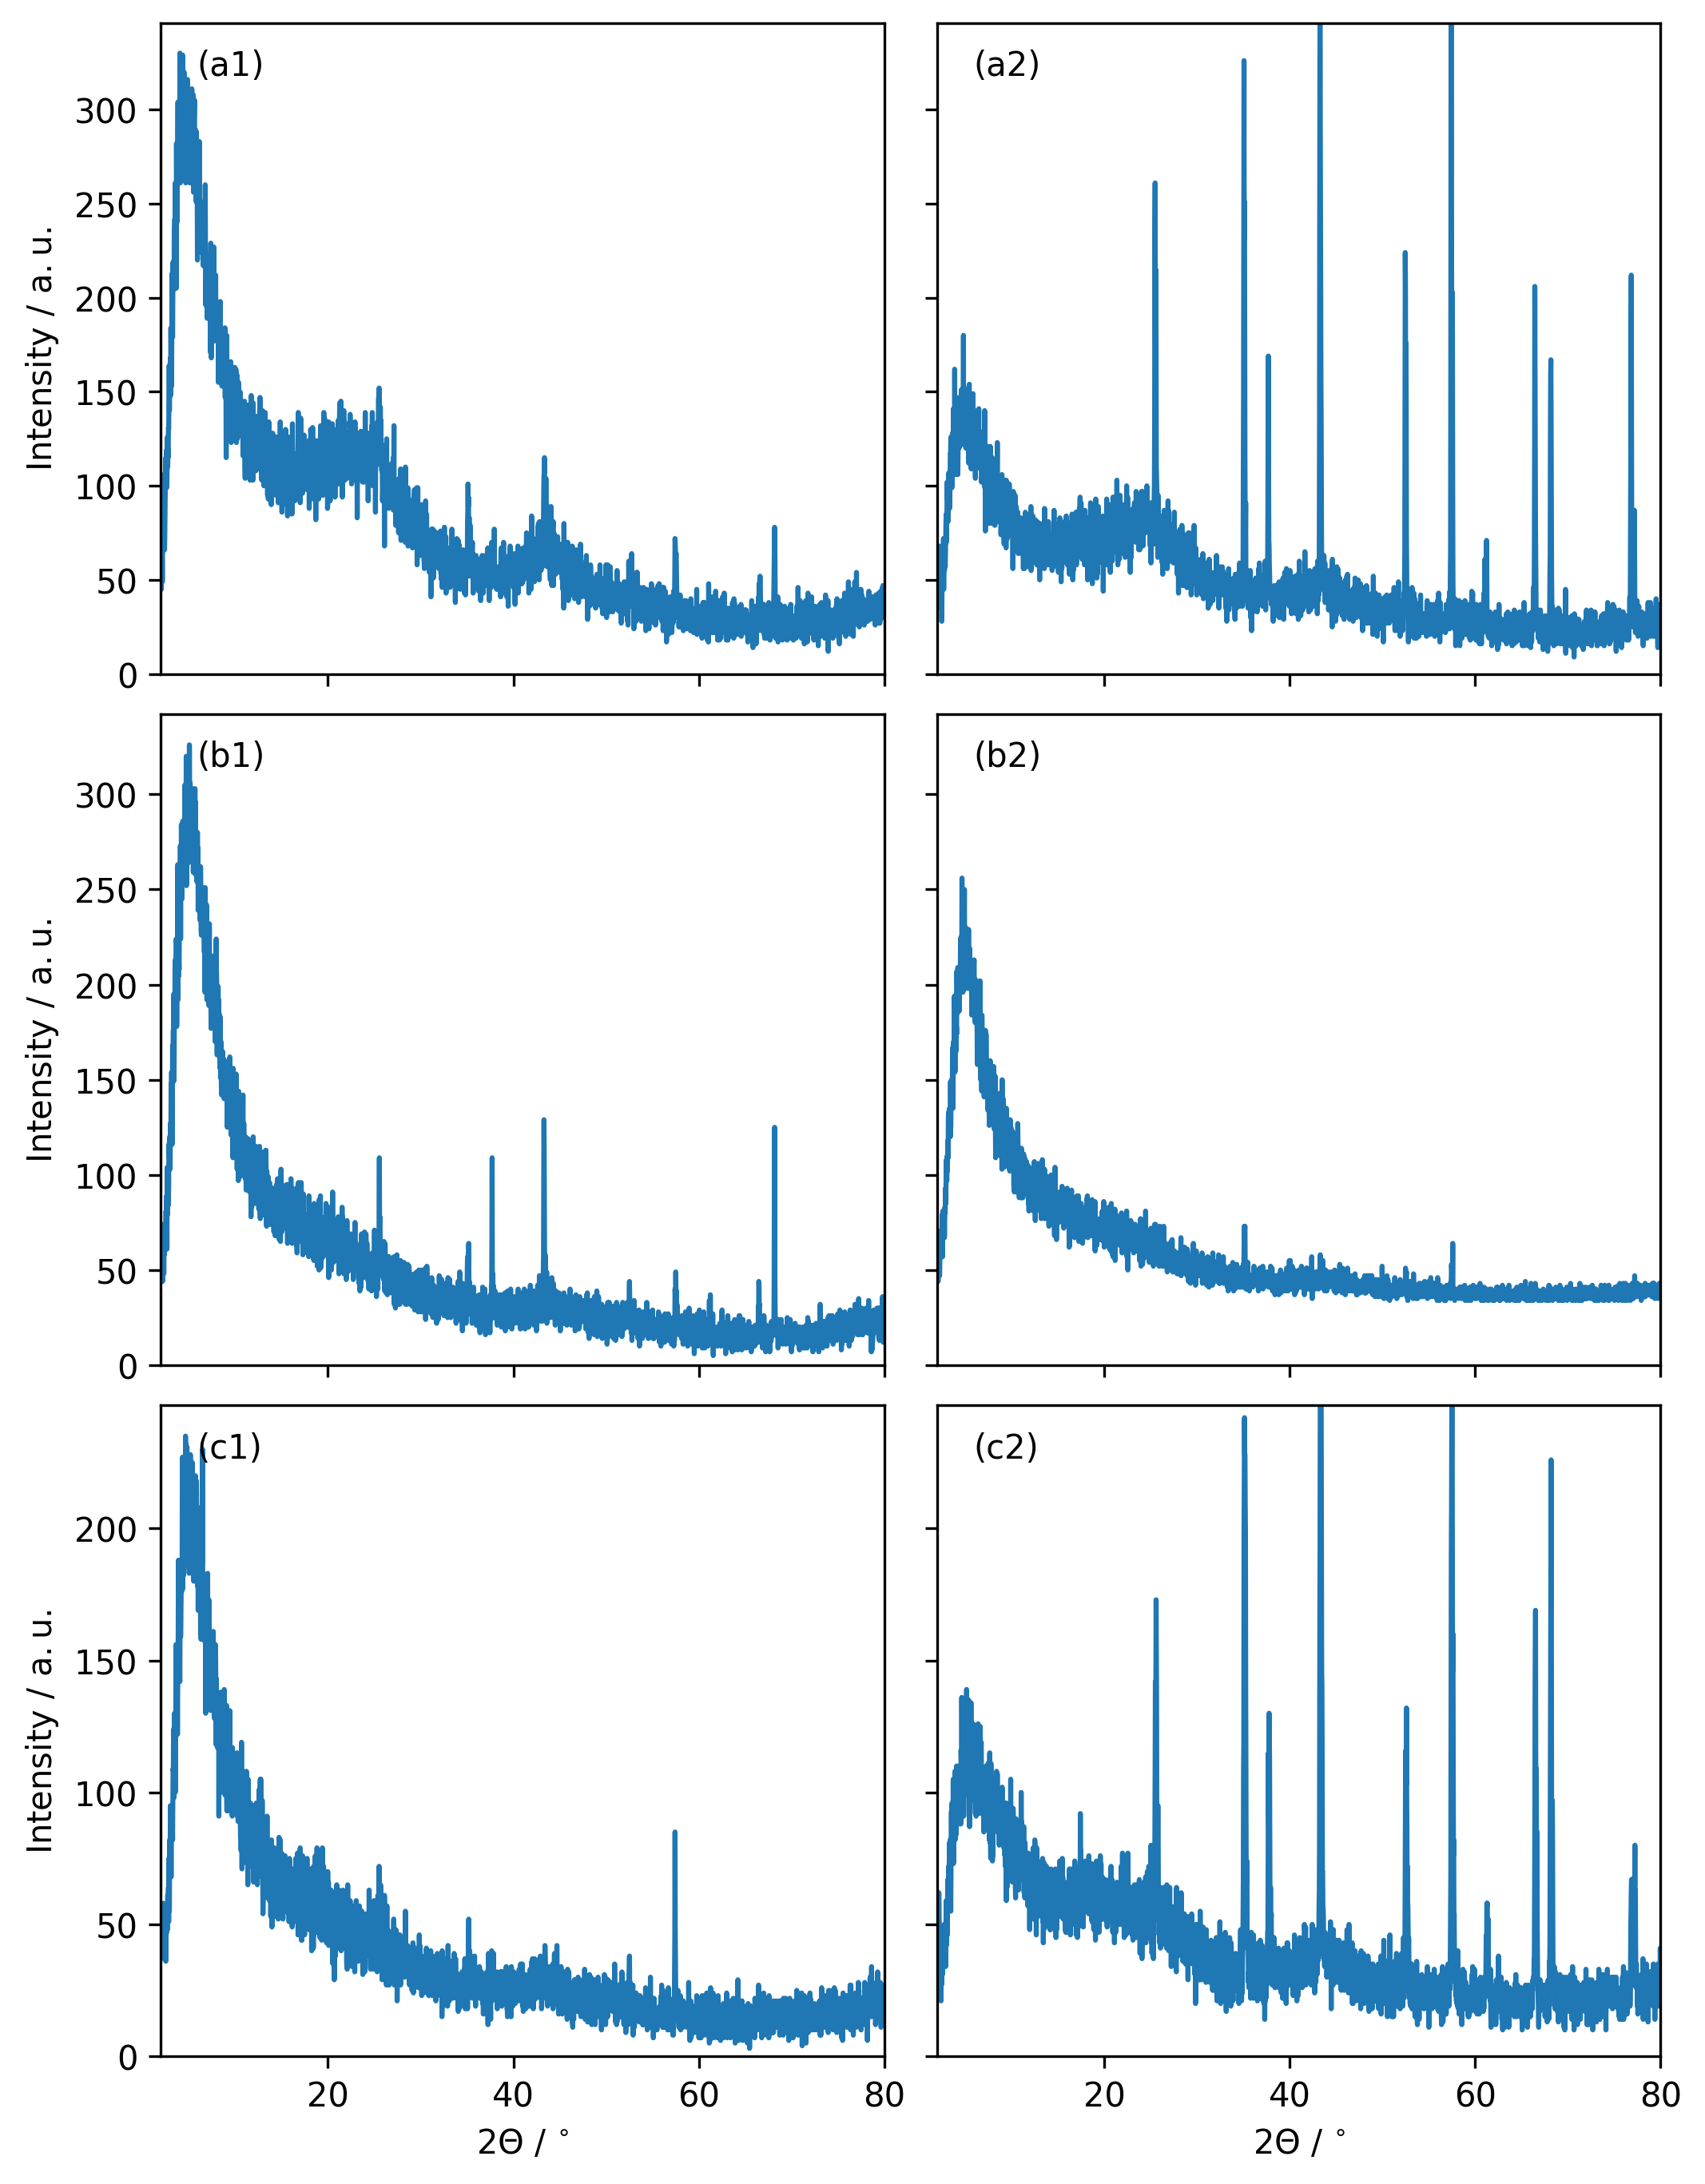
\includegraphics[width=\columnwidth, keepaspectratio]{4-cbs/figs/xrd_KOH.png}
    \caption{P-XRD spectra for samples hC-4600 (a1), hD-4600 (a2), hC-4700 (b1), hD-4700 (b2), hC-4800 (c1), hD-4800 (c2).}
    \label{fig:xrd_KOH}
\end{figure}

\begin{figure}[h]
    \centering
    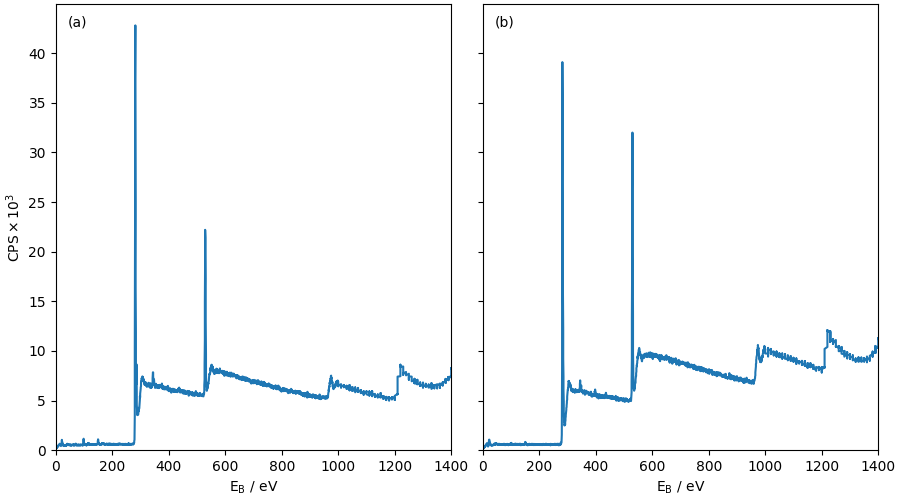
\includegraphics[width=\columnwidth, keepaspectratio]{4-cbs/figs/xps.png}
    \caption{XPS spectra for samples hD-0700 (a) and hD-hydrochar (b).}
    \label{fig:cb_xps}
\end{figure}

\begin{figure}[p]
    \centering
    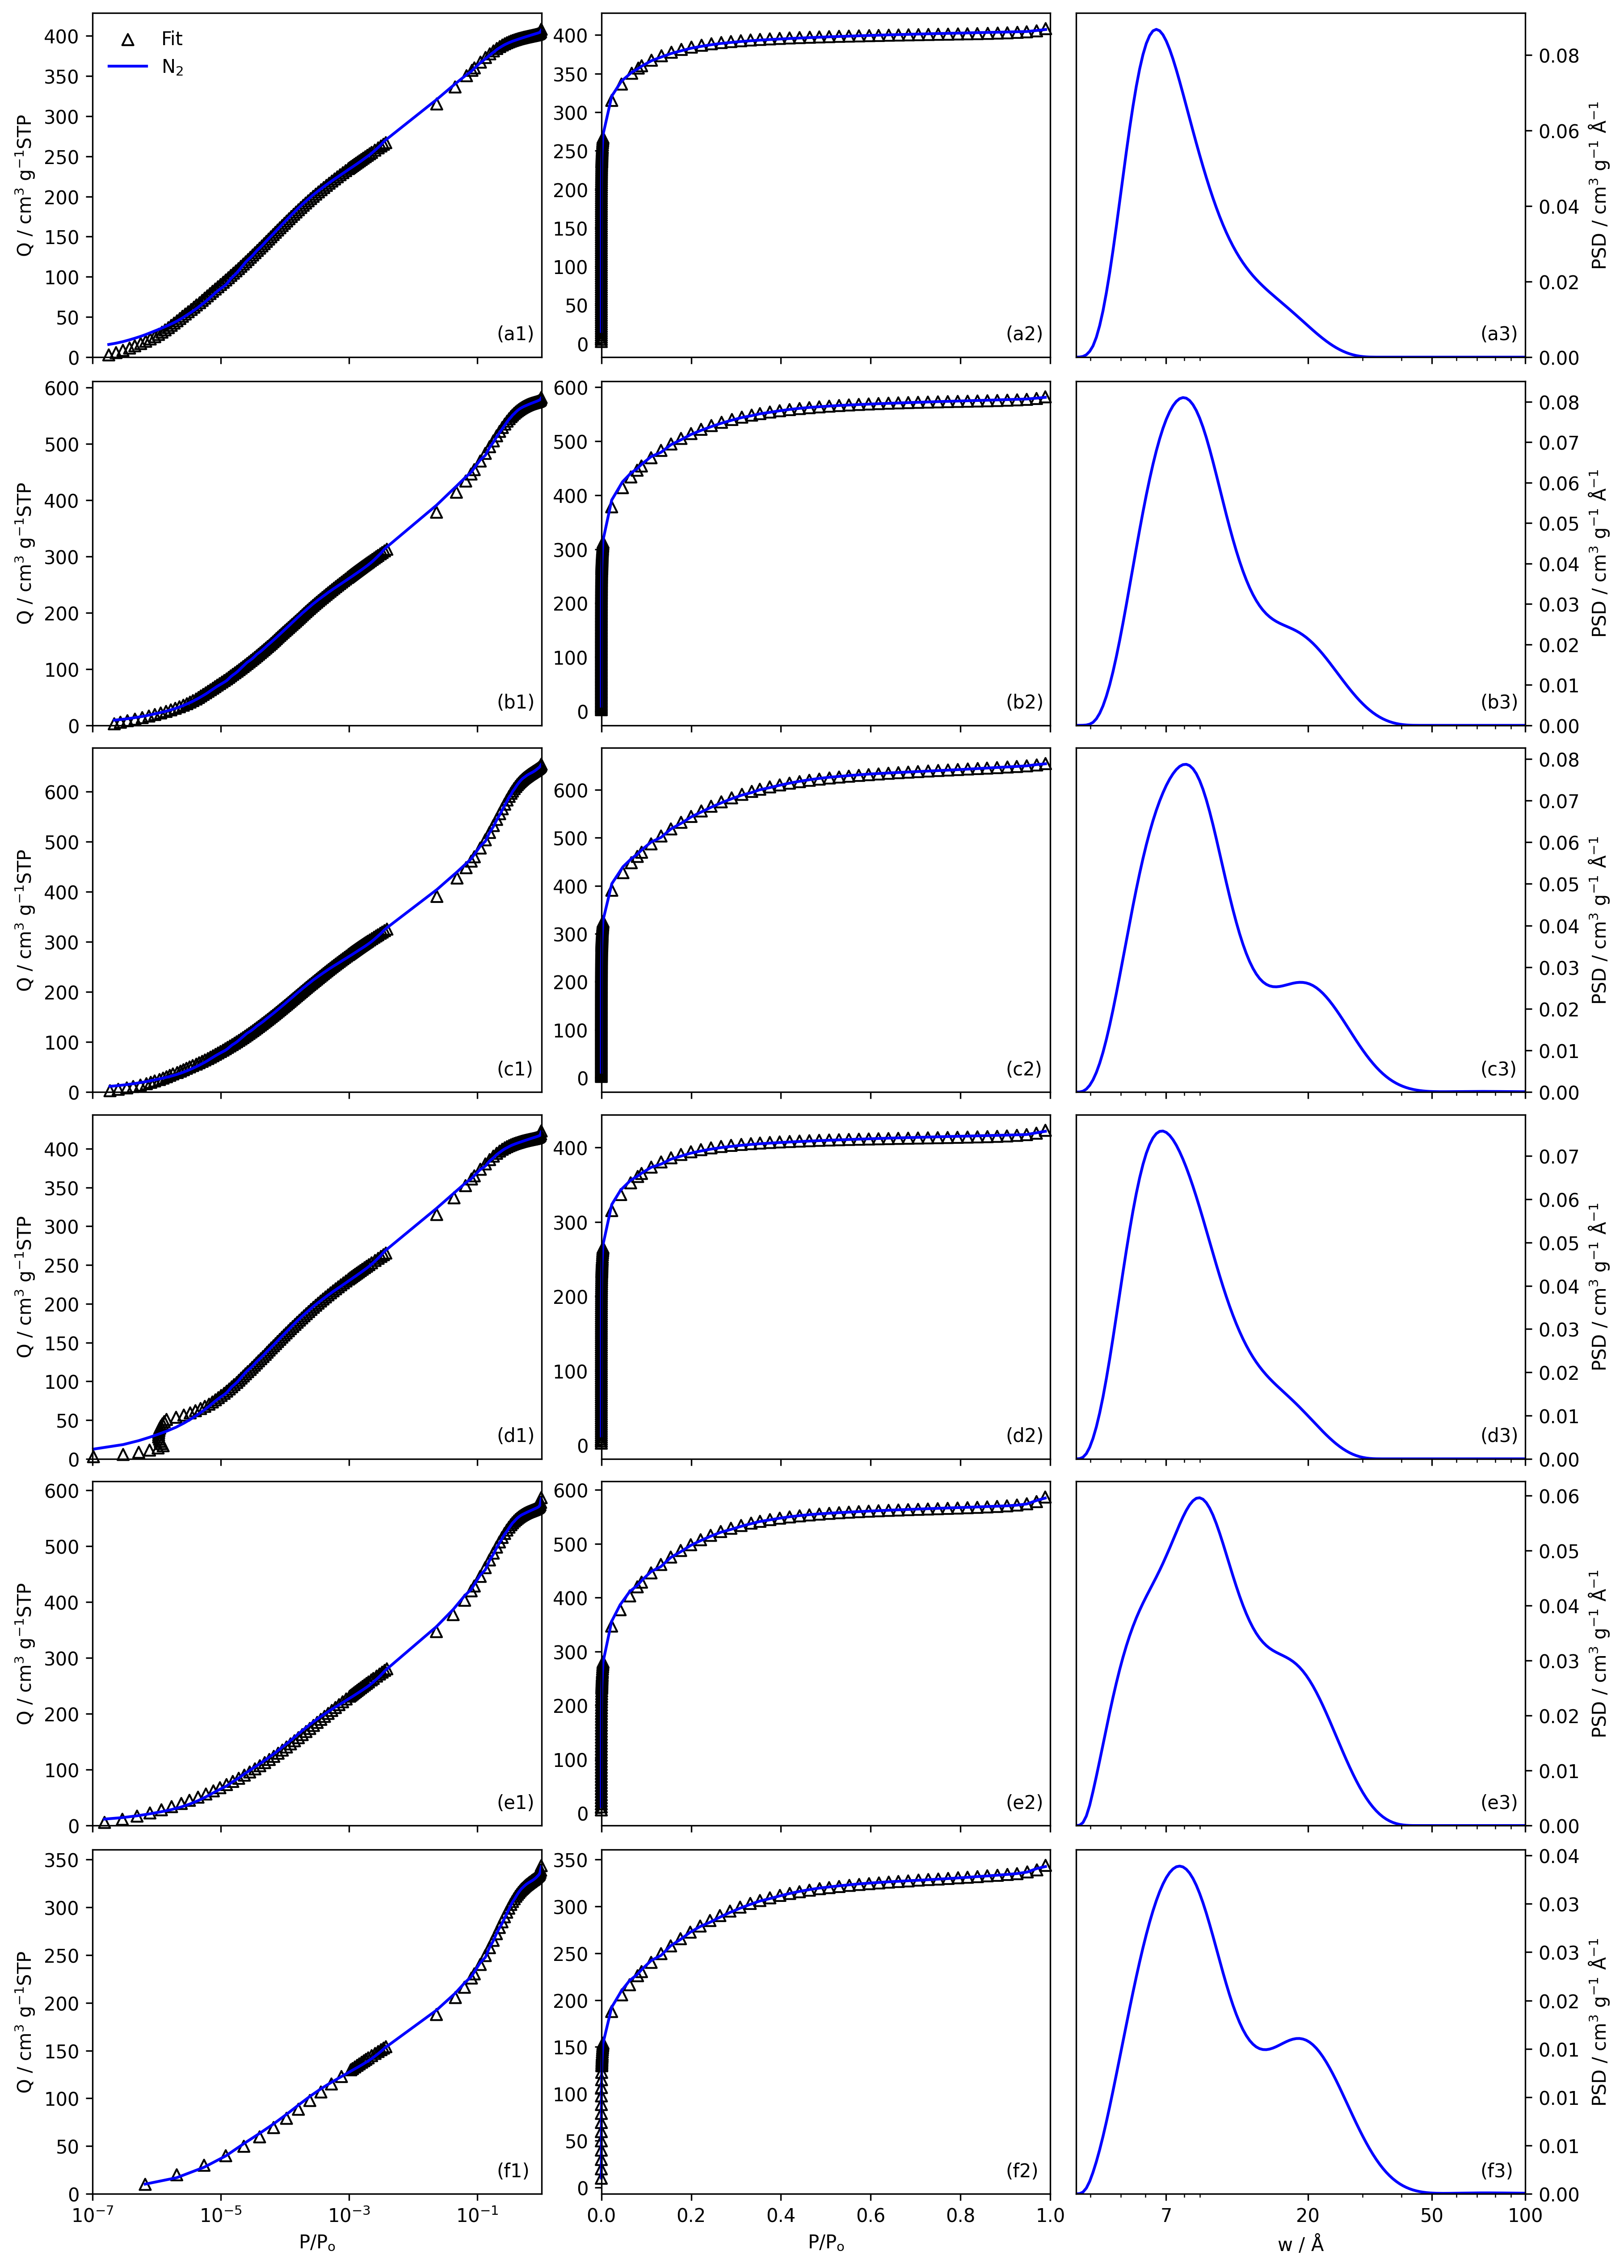
\includegraphics[width=\columnwidth, keepaspectratio]{4-cbs/figs/CB-4TTT_isopsd.png}
    \caption{Fits to \ce{N2} isotherms with logarithmic (a) and linear (b) relative pressure scale, and resultant differential PSDs (c) for samples hC-4600, hC-4700, hC-4800, hD-4600, hD-4700, hD-4800 in order in rows (1-6).}
    \label{fig:4TTT_psdisofull}
\end{figure}

\begin{figure}[p]
    \centering
    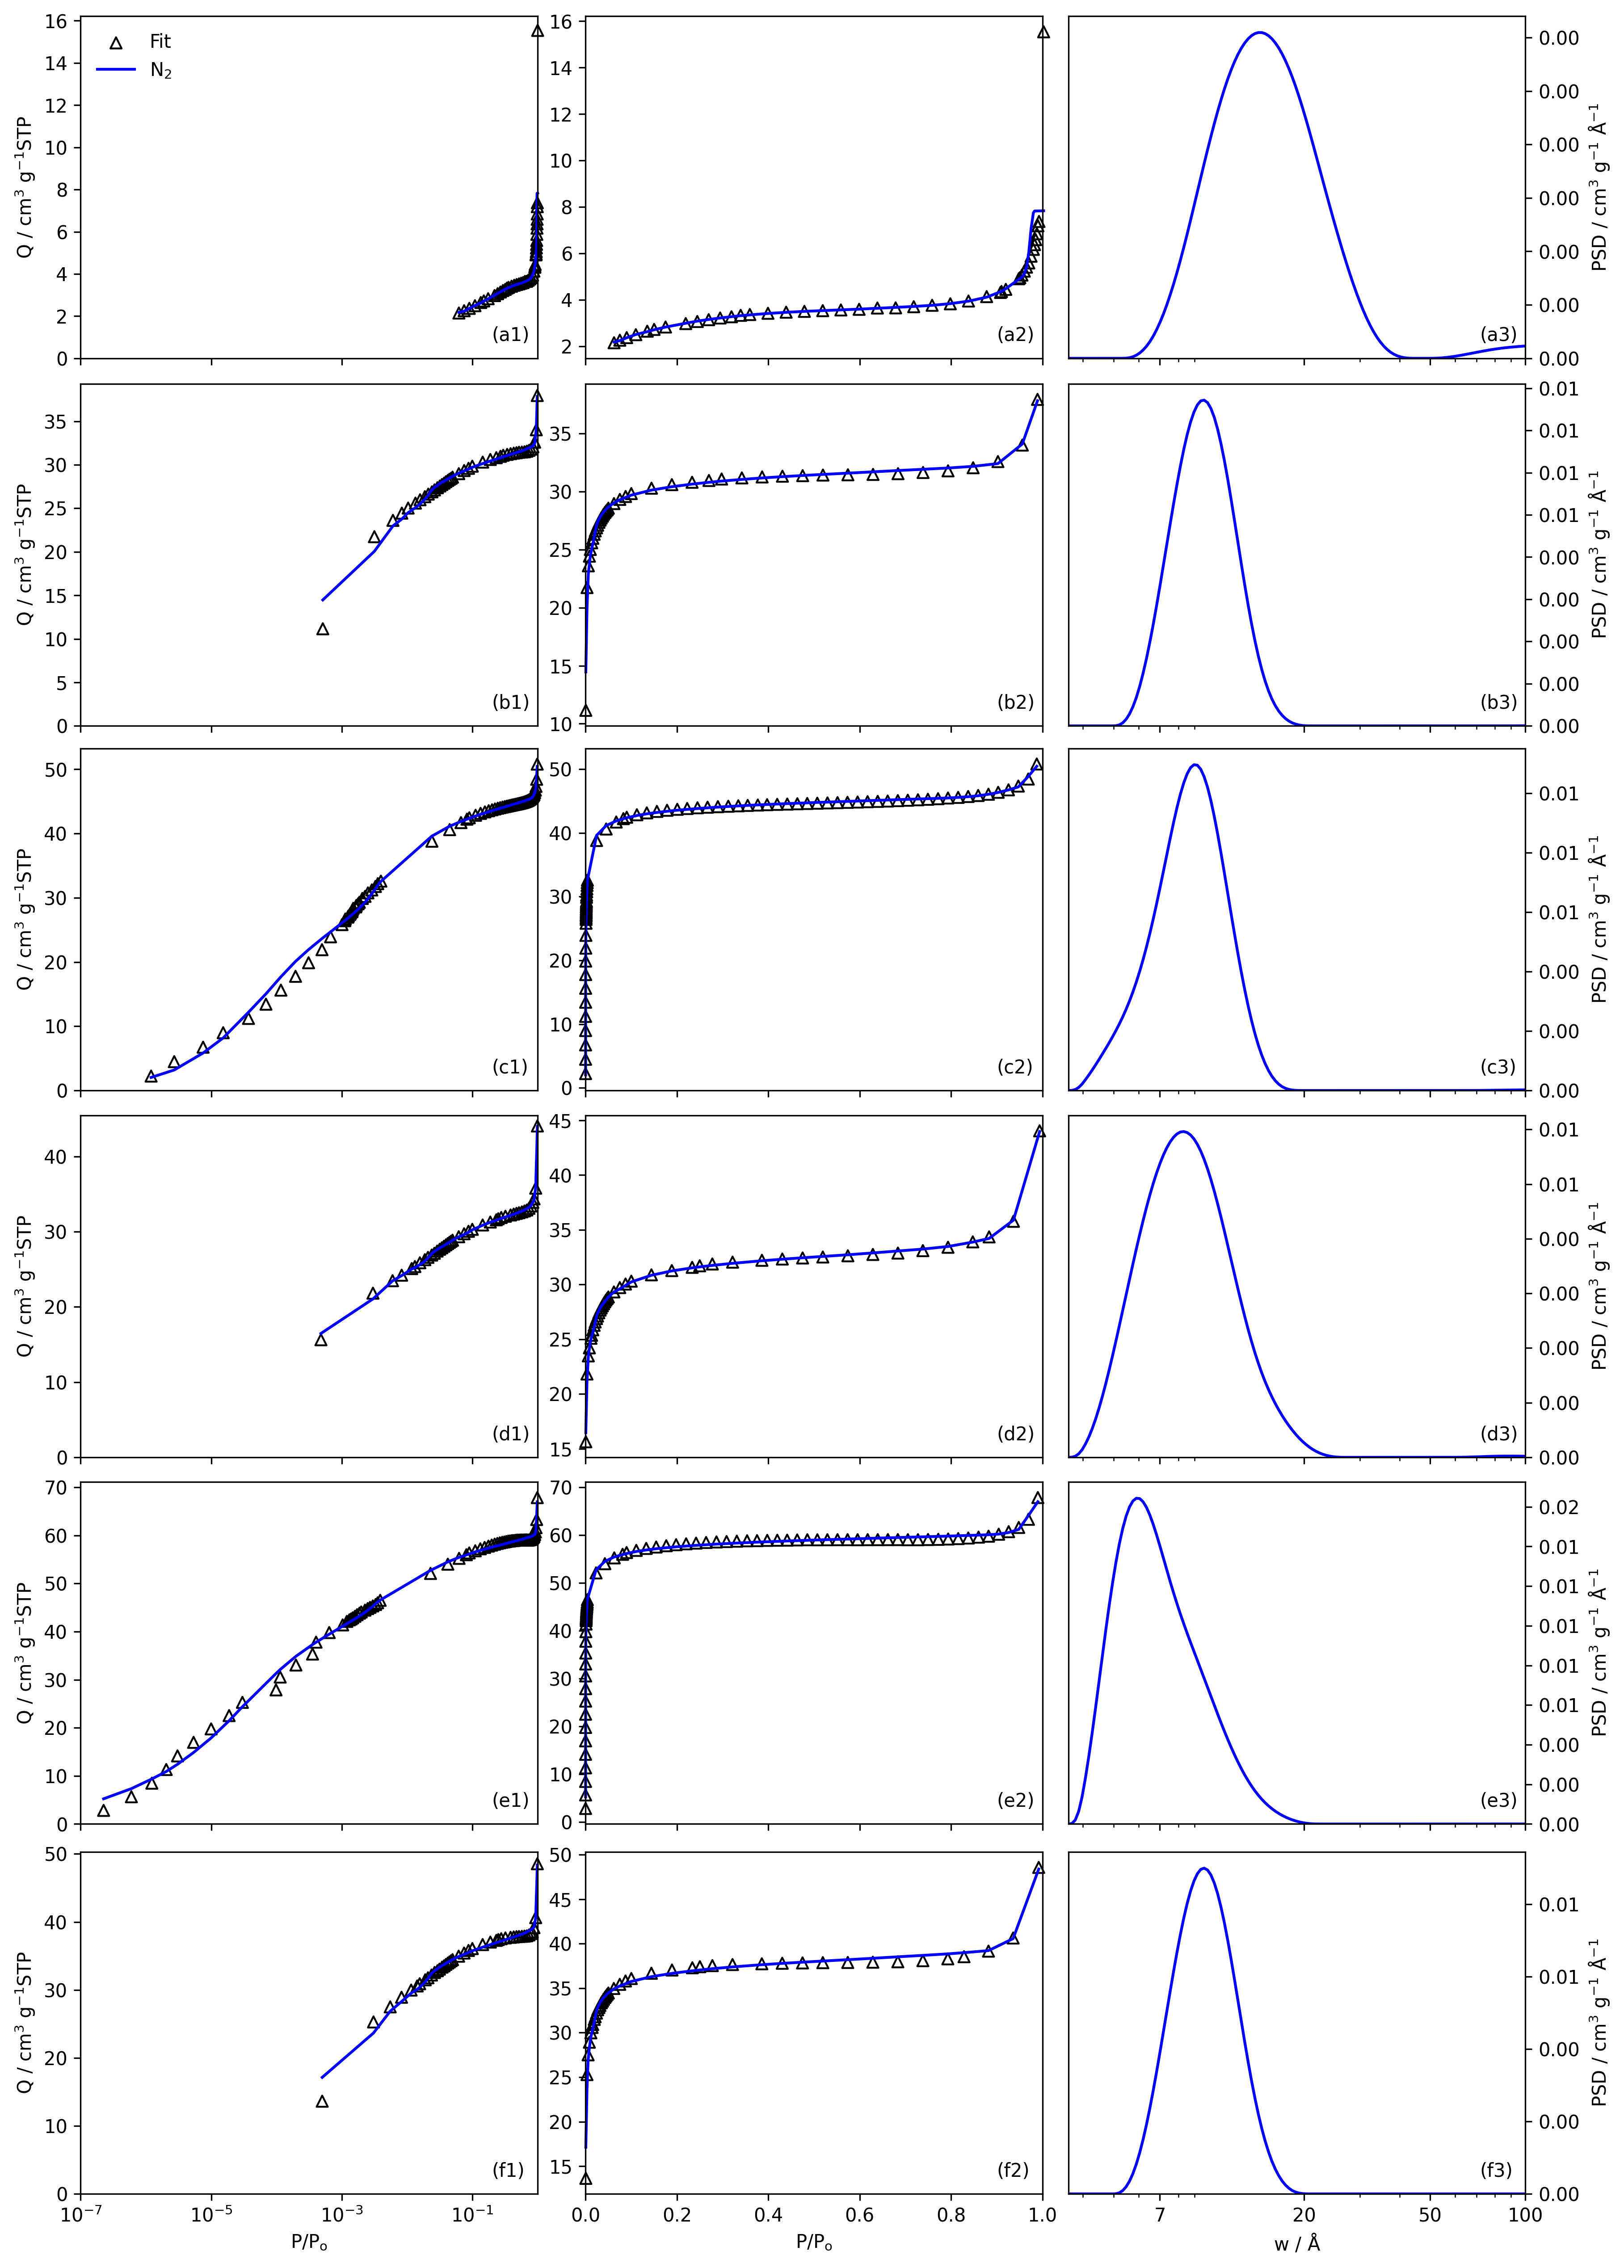
\includegraphics[width=\columnwidth, keepaspectratio]{4-cbs/figs/CB-0TTT_isopsd.png}
    \caption{Fits to \ce{N2} isotherms with logarithmic (a) and linear (b) relative pressure scale, and resultant differential PSDs (c) for samples hD-0600, hD-0700, hD-0800, hD-0600$'$, hD-0700$'$, and hD-0800$'$ in order in rows (1-6).}
    \label{fig:0TTT_psdisofull}
\end{figure}


\begin{figure}[h]
    \centering
    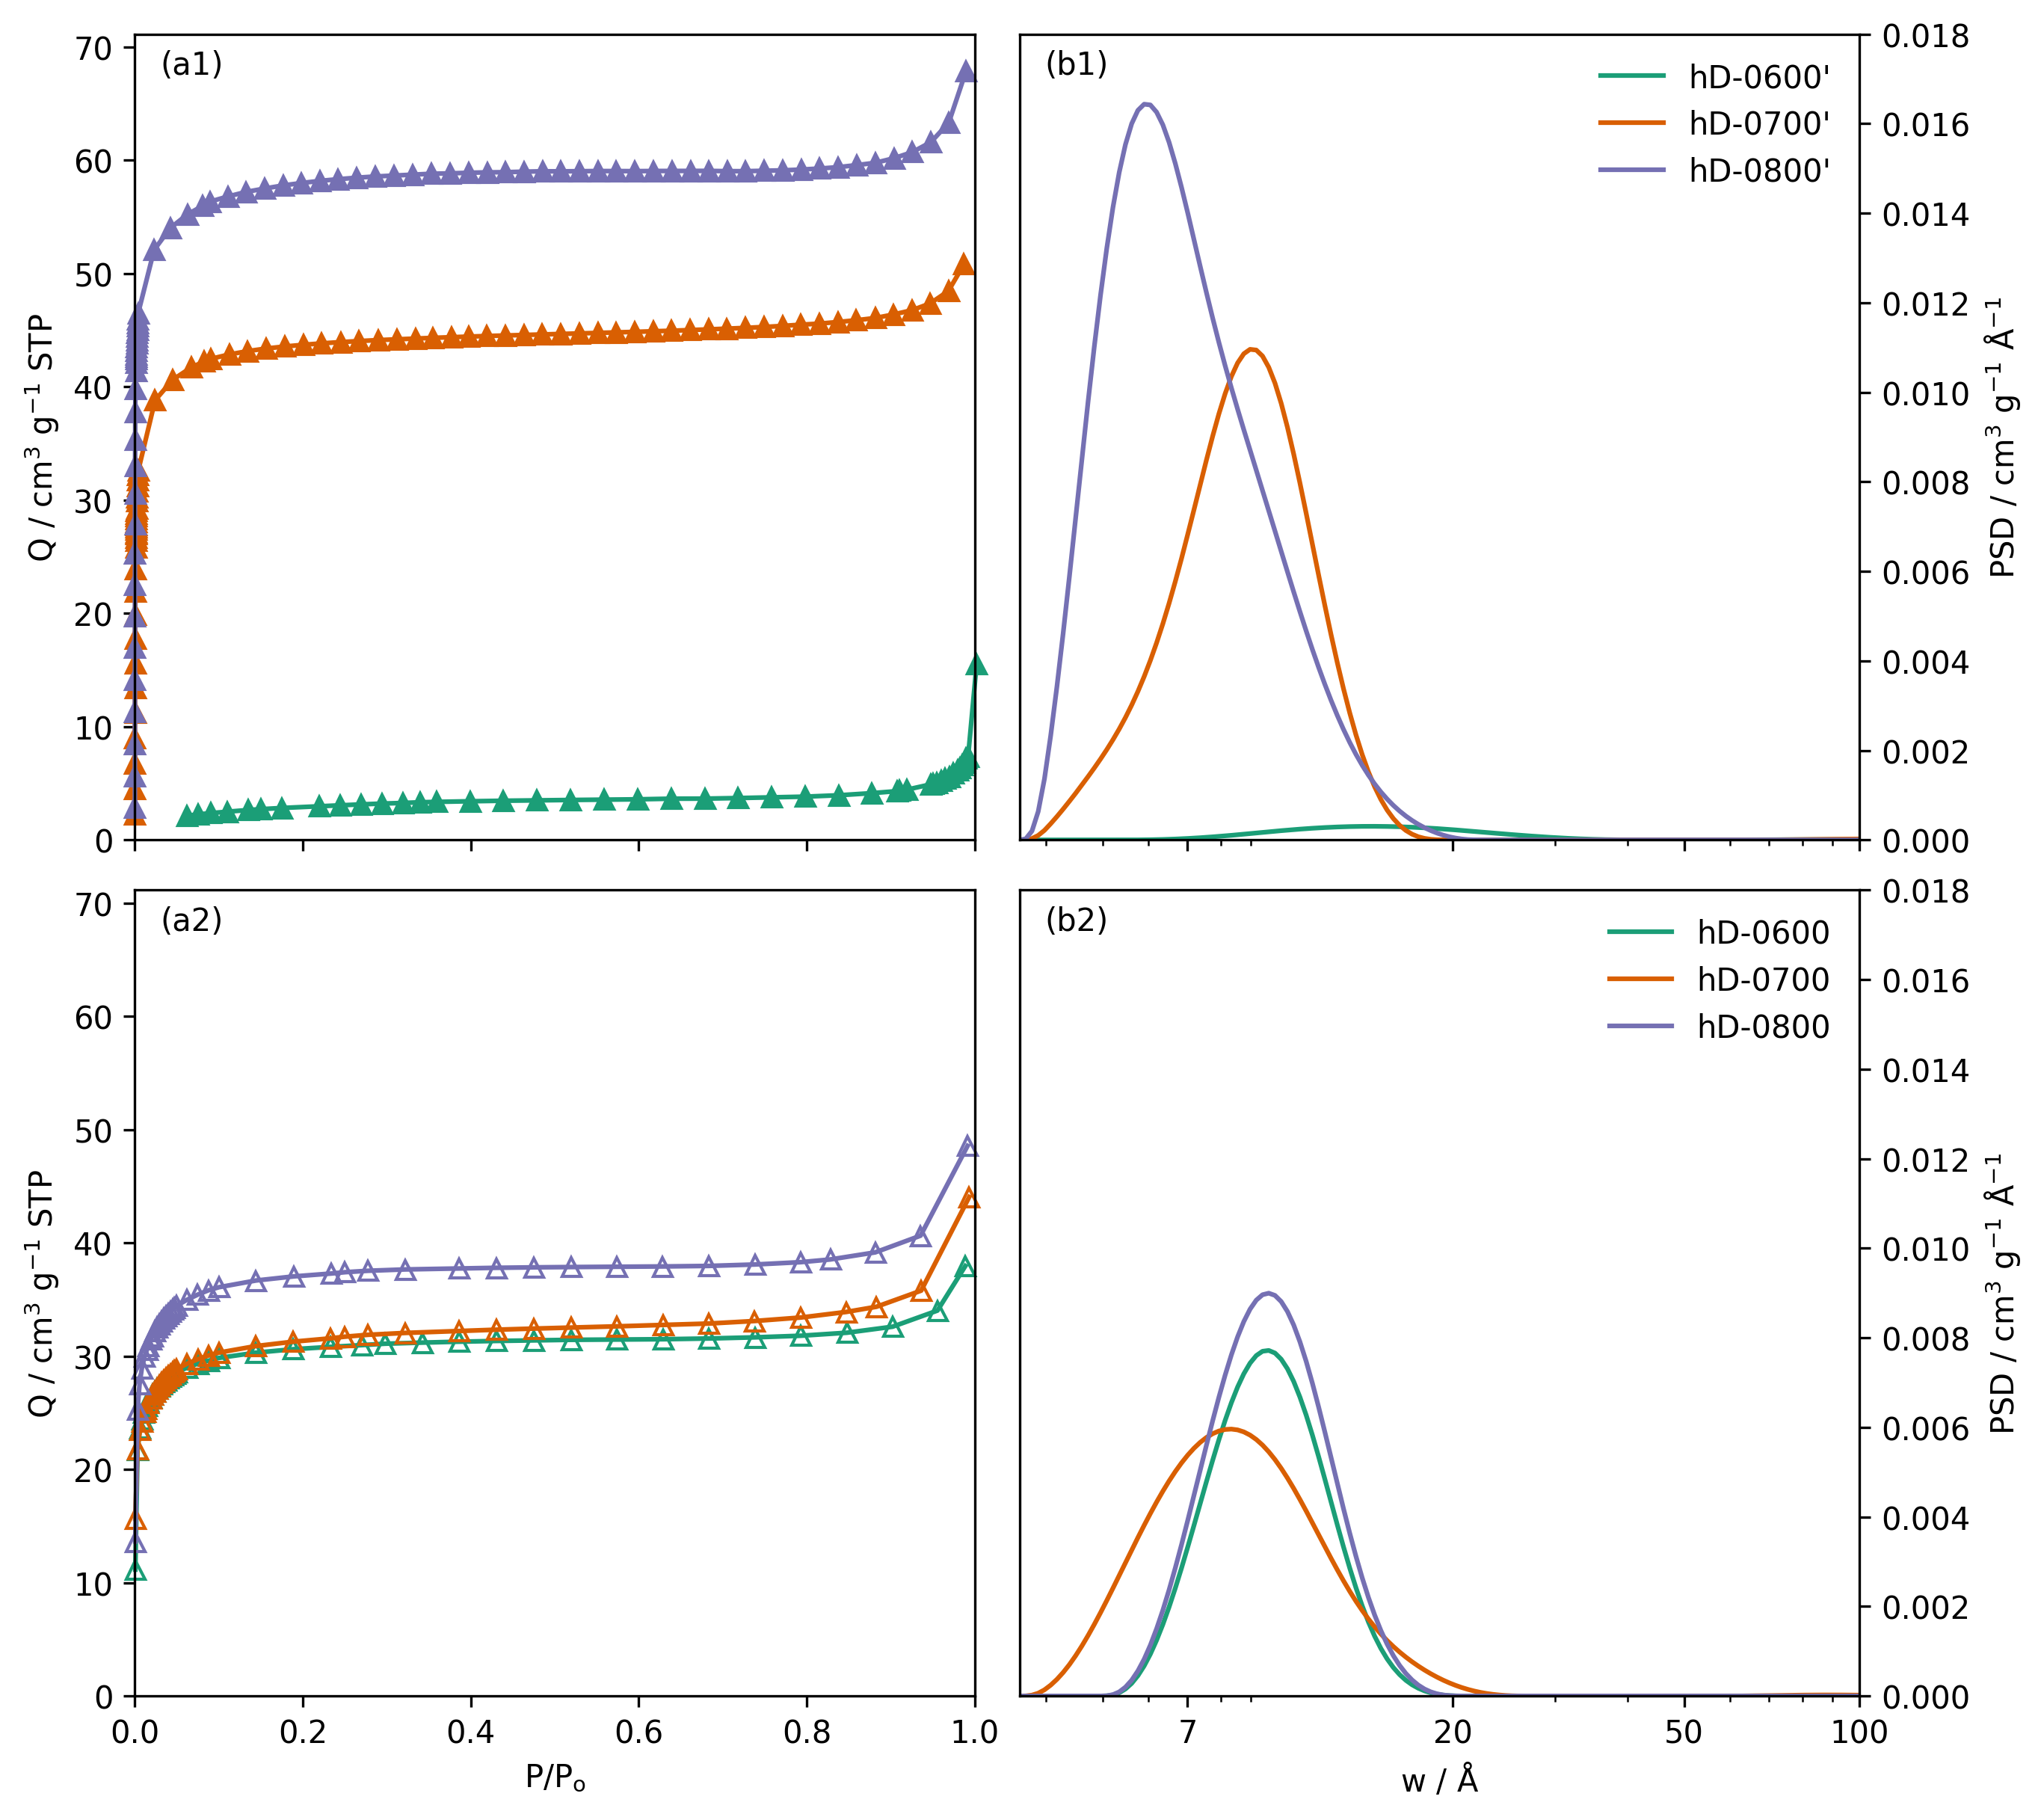
\includegraphics[width=\columnwidth, keepaspectratio]{4-cbs/figs/0TTT_n2_isotherms.png}
    \caption{Isotherms and resultant PSDs for samples hD-0\textit{TTT} and hD-0\textit{TTT}$'$.}
    \label{fig:0TTT_psdiso}
\end{figure}


\begin{figure}[h]
    \centering
    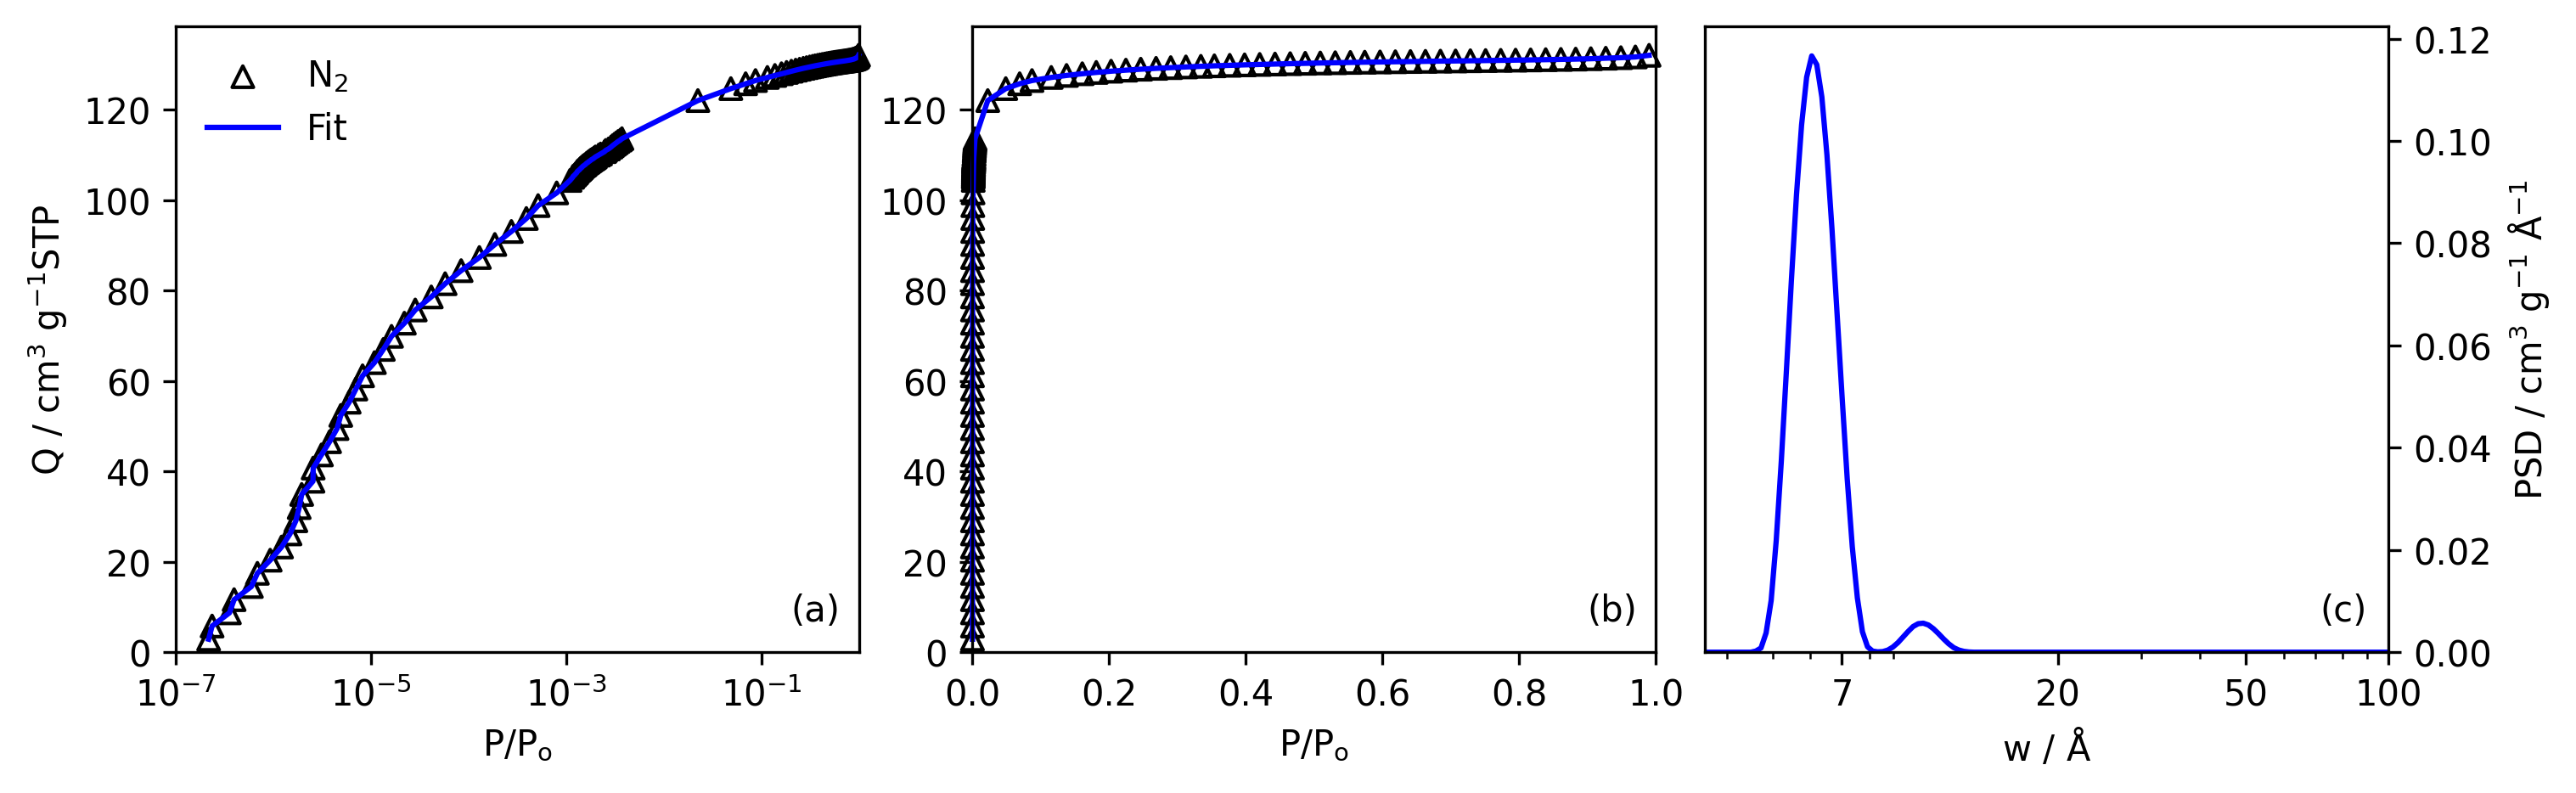
\includegraphics[width=\columnwidth, keepaspectratio]{4-cbs/figs/CA_iso_psd.png}
    \caption{Fits to \ce{N2} isotherms with logarithmic (a) and linear (b) relative pressure scale, and resultant differential PSDs (c) for the cellulose acetate derived sample CA-0800.}
    \label{fig:CA_psdiso}
\end{figure}

\clearpage
\begin{table}[h]
    \centering
    \caption{Porosity of CA-0800}
    \label{tb:CA_porosity}
    \begin{tabularx}{0.9\textwidth}{llllll}
    \toprule
        \multicolumn{2}{l}{$\mathbf{A_{BET}\ /\ m^2\ g^{-1}}$}  & \multicolumn{2}{l}{\textbf{Pore volume} / $\mathbf{cm^3\ g^{-1}}$} & \multicolumn{2}{l}{\textbf{Pore size / \AA}} \\
    \midrule
    522 & (491) & 0.20 & (0.19) & 6 \\
    \bottomrule
    \end{tabularx}
\end{table}

\end{subappendices}
\chapter{Turbostratic carbons II: Impregnation methods}
\label{ch:impregnation}

\newpage
\section*{Abstract}
In recent years, various researchers have investigated alternative methods of introduction of oxidative chemical \gls{porogen} to precursor in the synthesis of \glspl{activated carbon}. These differ from the standard physical mixing method in that they attempt to increase the homogeneity of the precursor-\gls{porogen} mixture while simultaneously decreasing distances between \gls{porogen} and precursor atoms. These techniques include solution impregnation and the carbonisation of organic salts. Such techniques are collectively termed as impregnation techniques for the purposes of this chapter, and have been shown to yield more precise control over pore size, geometry, and pore network connectivity as well as showing promise in facilitation development of improved microporosity.

What is lacking in these studies is insight into the effect of the relative quantity of impregnated \gls{porogen} as well as activation temperature on the pore structure and elemental composition of the derived porous carbons. Thus, this chapter reports the investigation of these variables by two means, (i) hydrothermal impregnation of \ce{KOH} into \acrfull{sd} followed by pyrolysis, and (ii) carbonisation of \acrfull{nc} at varying degrees of substitution. It was found that in the case of the \acrshort{sd}-derived materials, \ce{C} content is drastically improved by this technique relative to more `traditional' methods. In addition at a \ce{KOH}:\acrshort{sd} ratio of \num{2.00}, a carbon with unusually low bulk density (\qty{\sim0.031}{\gram\per\cm\cubed}),  and high mesoporosity (\qty{73}{\percent} by surface area) is produced. As for \acrshort{nc}-derived carbons, in many cases a two-phase highly oxygen-rich product was produced. These properties appear to be a function of both the amount of \ce{Na} in the precursor, as well as activation temperature. Network connectivity and/or pore geometry in the carbons also appears to be a result of these two variables. This work provides scope for investigation of the pore formation mechanisms of these highly unusual carbons.

\newpage

\section{Introduction}
Most commonly in the synthesis of activated carbons \glspl{porogen} are added to precursors by physical mixing - i.e. some combination of grinding and stirring - with the precursor.\citep{Aljumialy2020Porous, Blankenship2017Cigarette, Altwala2020Predictable, Sevilla2016Highly} As mentioned in \textbf{section 4.1.1.} of \ref{pub:review} an alternative technique is to impregnate the precursor with a (typically aqeuous) solution of \gls{porogen}.\citep{Botome2017Preparation, Ge2019Highly, Adlak2021Physicochemical, Shi2021Copper, Han2021Mulch} While there is scant evidence that solution impregnation has better outcomes over physical mixing in terms of porosity development, the rationale of the former technique is that the \gls{activating agent} will be more evenly distributed throughout the precursor thus providing more homogenous porosity in the product however there is as yet no study to support this. 

A further method using oxidative chemical activation is so-called organic salt carbonisation (again, see \ref{pub:review} \textbf{section 4.4.1.}) wherein the metal cation of an organic salt activates the carbonised precursor on pyrolysis. Reports, in particular from Sevilla \textit{et al.} show that this method allows for a high degree of tunability in carbon PSDs by changing the identity of the activating cation.\citep{Sevilla2013general, Tsumura2014Structure, Ferrero2015Mesoporous, Ferrero2016Efficient, Fuertes2015Hierarchical, Roberts2015Hierarchically, Yadav20123D, Yang2018Spontaneous} The majority of anions used in organic salt carbonisation are small molecules such as gluconate or citrate,\citep{Sevilla2013general, Yang2017Template, Sevilla2014Direct, Tsumura2014Structure, Ferrero2015Mesoporous, Ferrero2016Efficient, Fuertes2015Hierarchical, Yang2020Production, Fuertes2014One} however polymers have also been employed.\citep{Puthusseri20143D, Roberts2015Hierarchically, Yadav20123D, Hines2004Surface} 

The philosophy of these two emergent techniques (solution impregnation and organic salt carbonisation) for porogen-precursor mixing is that (i) the process can be simplified, (ii) porosity can be more readily controlled, and (iii) porosity is more homogeneous throughout the product. These effects are supposedly a result of both improved \gls{porogen}-precursor contact, and more homogeneous \gls{porogen} distribution. For the purposes of this chapter, mixing techniques with such goals are collectively termed `impregnation' methods. In terms of solution impregnation, thus far syntheses have only been reported wherein the precursor is mixed with the \gls{porogen} directly prior to pyrolysis.\citep{Botome2017Preparation, Ge2019Highly, Adlak2021Physicochemical, Shi2021Copper, Han2021Mulch, Boujibar2018CO2} That is, it has not been attempted to impregnate the \gls{porogen} at the \gls{htc} step. As such, herein the combined \gls{htc} and impregnation of \ce{KOH} on sawdust is examined. This technique is also inspired by the observation made by Zhang \textit{et al.} that the formation of \ce{K} salts with oxygen-rich moieties on the surface of calcined glucose is associated with improvements in ultramicroporosity.\citep{Zhang2019situ} \acrfull{sd} was chosen due to the dearth of literature surrounding carbons derived from the activation of hydrothermally carbonised sawdust,\citep{Balahmar2019Pre, Aljumialy2020Porous, Cox2017Ultra, Balahmar2015Generalized} making for easy comparison between the results of the technique studied in this chapter and more established techniques.

\begin{figure}[b!]
    \centering
    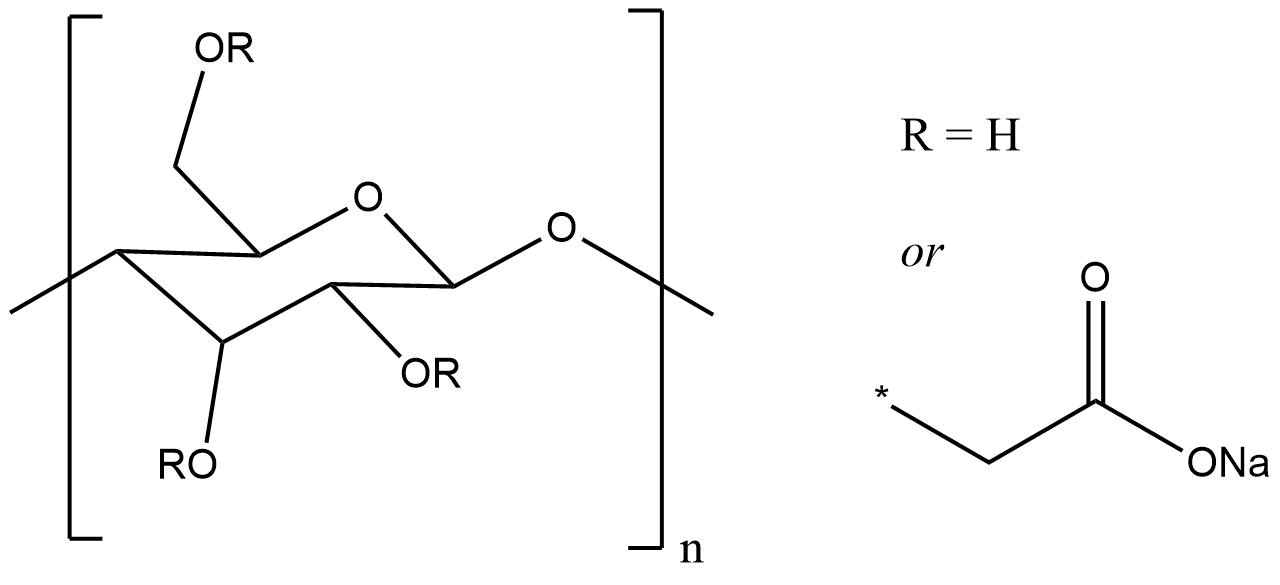
\includegraphics[width=0.8\columnwidth]{4-impregnation/figs/nc_structure.png}
    \caption{Structure of sodium carboxymethyl cellulose. \Acrfull{ds} is taken as the average number of sodium carboxymethyl groups (\ce{-CH2COONa}) per monomer.}
    \label{fig:nc_structure}
\end{figure}

On the other hand, while the porosity of carbons derived through organic salt carbonisation has been exploited through changing the cation,\citep{Sevilla2013general, Tsumura2014Structure, Ferrero2015Mesoporous, Ferrero2016Efficient, Fuertes2015Hierarchical, Roberts2015Hierarchically, Yadav20123D, Yang2018Spontaneous} the capacity for greater more precise control over porosity by changing the degree of substitution of a cation on a polymer chain has not yet been explored. In studies using physical mixing, the \gls{porogen}:precursor weight ratio is typically reported.\citep{Altwala2020Predictable, Adeniran2015Compactivation, Blankenship2017Cigarette, Sevilla2016green, Ludwinowicz2015Potassium, Deng2015Inspired, Alhamed2015Preparation, Hu2003simple} As discussed in \ref{pub:review}, \textbf{section 2.1.2.} oxidative chemical activation primarily relies on redox reactions between \ce{C} and the \gls{porogen}, thus knowing the exact stoichiometric  \gls{porogen}:\ce{C} ratio may provide a route to understanding the precise effects of \gls{porogen} concentration on carbon porosity requires information as to the composition of the precursor. To this end, this study also investigates \acrfull{nc} (structure shown in figure \ref{fig:nc_structure}) as a precursor to activated carbon. The \gls{porogen} in this case is the sodium carboxymethyl group, and the \gls{porogen}:precursor ratio is controlled by the \acrfull{ds}.

\section{Synthesis}
Sawdust-derived carbons were made by incorporating \ce{KOH} at weight ratios between \numlist{0.00;2.00} into the \gls{htc} step, drying the resultant slurry overnight at \qty{100}{\degreeCelsius} and then activating at \qty{800}{\degreeCelsius} as usual. \Gls{htc} occured at \qtylist[list-units=single]{200;250;300}{\degreeCelsius}. These sawdust-derived \glspl{hydrochar} are designated SA\textit{x.xx-HHH} where the prefix SA indicates activated sawdust, \textit{x.xx} is the KOH:sawdust ratio and \textit{HHH} is the \gls{htc} temperature. All samples were washed in the normal manner following activation. The hydrothermally carbonised intermediates were also isolated and washed - they are designated  SH\textit{x.xx-HHH} to differentiate them from the activated samples.

Additionally, sodium carboxymethyl cellulose (see figure \ref{fig:nc_structure}) was used as a precursor for direct (without \gls{htc}) activation.  Samples are designated as NC\textit{x.x-TTT} where \acrshort{nc} indicates sodium carboxymethyl cellulose, \textit{x.x} is the \acrshort{ds}, and \textit{TTT} is the activation temperature. Values for \textit{x.x} were \numlist{0.0;0.7;0.9;1.2} and \textit{TTT} was \qtylist[list-units=single]{600;700;800}{\degreeCelsius}.

\section{Results \& Discussion}
\subsection[Hydrothermal Sawdust KOH-impregnation]{Hydrothermal Sawdust \ce{KOH}-impregnation}
\label{ss:sd_results}

Eleven SH\textit{x.xx-HHH} samples were produced from the sawdust precursor. In the case of \textit{x.xx} \num{>0.00}, removal of \ce{K} salts \textit{via} washing resulted in the sole product being small amounts of flakey carbonaceous matter that was difficult to isolate as an intermediate. As a result, compositional and porosimetric analysis was difficult to achieve. Furthermore, extensive washing appears to remove extremely fine particles which may have some function in the subsequent pyrolysis step. The three \glspl{hydrochar}, SH0.00-\textit{HHH} were much easier to isolate and analyse. The eleven \glspl{turbostratic carbon} (SA\textit{x.xx-HHH}) were the typical black powders, however SA2.00-250 was very diffuse and clearly has a much lower density relative to the other samples and indeed to that of typical activated/\glspl{turbostratic carbon}.

\subsubsection{Composition}

CHN elemental microanalysis was used to determine the composition of sawdust precursor and derived carbons; results are show in table \ref{tb:sa_chn}. \acrshort{tga} shows that all samples are fully carbonaceous, i.e. there are no residual \ce{K} compounds present after washing - see appendix, figure \ref{fig:SD_tga}. Thus, in the CHN analysis, the remainder of the sum of \ce{C}, \ce{H} and \ce{N} gravimetric concentrations is assumed to be made up by \ce{O} in table \ref{tb:sa_chn}. In addition, for all carbons there is a single burn-off event at \qty{600}{\degreeCelsius}, as reported previously both for carbons prepared directly from sawdust or from sawdust-derived \gls{hydrochar}.\citep{Balahmar2017Biomass} Therefore, the thermal stability of carbons derived from sawdust does not seem to be significantly effected by the quantity (or even presence) of \ce{KOH} as a \gls{porogen}, the method of preparing the precursor, or the method of introducing \ce{KOH} to the precursor.

\begin{table}[b!]
    \caption{Composition of SA\textit{x.xx-TTT} carbons according to elemental microanalysis. \ce{O} content is the remaining \unit{\wtpercent} after consideration of the \ce{C}, \ce{H}, and \ce{N}.}
    \label{tb:sa_chn}
    \begin{tabularx}{\textwidth}{lXXXXXX}
    \toprule
        \textbf{Sample} & \multicolumn{4}{c}{\textbf{Concentration / \unit{\wtpercent}}} & \multicolumn{2}{c}{\textbf{Atomic ratio}} \\
        & \textbf{C} & \textbf{H} & \textbf{N} & \textbf{O} & \textbf{O/C} & \textbf{H/C} \\
    \midrule
        \textbf{\acrshort{sd}} & 45 & 6 & 1 & 48 & 0.80 & 1.62 \\
        \\
        \textbf{SA0.00-200} & 87 & 1.4 & 1.7 & 11 & 0.09 & 0.19 \\
        \textbf{SA0.50-200} & 88 & 0.44 & 0.03 & 12 & 0.10 & 0.06 \\
        \textbf{SA1.00-200} & 90 & 0.15 & 0.94 & 8.8 & 0.07 & 0.02 \\
        \\
        \textbf{SA0.00-250} & 85 & 0.94 & 0.33 & 14 & 0.12 & 0.13 \\
        \textbf{SA0.25-250} & 87 & 0.04 & 0.05 & 13 & 0.12 & 0.13 \\
        \textbf{SA0.50-250} & 93 & 0.00 & 0.52 & 6.2 & 0.05 & - \\
        \textbf{SA1.00-250} & 90 & 0.00 & 0.00 & 9.6 & 0.08 & - \\
        \textbf{SA2.00-250} & 93 & 0.00 & 0.00 & 7.5 & 0.06 & - \\
        \\
        \textbf{SA0.00-300} & 86 & 0.89 & 0.55 & 12 & 0.11 & 0.12 \\
        \textbf{SA0.50-300} & 91 & 0.09 & 0.15 & 8.6 & 0.07 & 0.01 \\
        \textbf{SA1.00-300} & 92 & 0.14 & 0.00 & 7.4 & 0.06 & 0.02 \\
    \bottomrule
    \end{tabularx}
\end{table}

The elemental composition of the sawdust is similar to that previously reported by the Mokaya group.\citep{Balahmar2019Pre, Balahmar2017Biomass} Carbons derived from the slurries formed \textit{via} \gls{htc} at \qtylist[list-units=single, list-final-separator={or }]{250;300}{\degreeCelsius} without the use of \ce{KOH} have slightly lower \ce{C} contents than their \ce{KOH}-activated counterparts, and retained some \ce{H} and \ce{N}. On the other hand, \ce{KOH}-activated samples with \ce{KOH}:\acrshort{sd} mass ratio \num{>0.25} are at least \qty{90}{\percent} carbon with the heteroatoms - excluding \ce{O} - almost completely removed. On the other hand, SA0.00-200 has a very similar \ce{O}/\ce{C} atomic ratio to SA0.50-200. This indicates that at some \gls{htc} temperature between \qtylist[list-units=single]{200;250}{\degreeCelsius}, \ce{KOH} facilitates the breakdown of \ce{O}-rich moieties in the sawdust, resulting in their removal during the activation step. Further, the addition of \ce{KOH} only significantly facilitates this degradation once \ce{KOH}:\ce{C} mass ratio is greater than 0.25. The \ce{O}/\ce{C} atomic ratios of the SA\textit{x.xx}-250 ($x.xx>0.00$) carbons are  lower than those of previously reported carbons derived by the sequential \gls{htc} at \qty{250}{\degreeCelsius} and activation with \ce{KOH} at \qty{800}{\degreeCelsius}. In their report, Balahmar and Mokaya find that the the lowest \ce{O}/\ce{C} (\num{0.12}) was achieved at a \ce{KOH}:\gls{hydrochar} mass ratio of \num{4}.\citep{Balahmar2017Biomass} Thus, the inclusion of \ce{KOH} in the \gls{htc} step provides for a route to a more carbon-rich material, without necessitating the use of higher quantities of \ce{KOH}.

\subsubsection{Porosity}

It was initially attempted to produce porous carbons \textit{via} \gls{htc} with a \ce{KOH} solution, i.e. without \gls{pyrolysis}. Unsurprisingly this proved ineffective as \gls{activation} typically requires temperatures in excess of \qty{400}{\degreeCelsius}.\citep{Sevilla2014Energy, Blankenship2022Modulating} $A_{BET}$ of these samples (i.e. SH\textit{x.xx-HHH}) was not in excess of \qty{10}{\metre\squared\per\gram}. As for the pyrolised samples, porosity was reasonable, with $A_{BET}$ of least \qty{300}{\metre\squared\per\gram} for samples synthesised without \ce{KOH}, and above \qty{990}{\metre\squared\per\gram} for the \ce{KOH}-activated samples. Full textural characteristics are shown in table \ref{tb:sa_porosity}, as well as the isotherms from which they are derived and \acrshortpl{psd} in figure \ref{fig:SA_n2_isotherms}.\footnote{Individual \glspl{psd} and the kernel fits they are derived from can be found in the appendix, figures \ref{fig:SAxxx-200_isopsd}-\ref{fig:SAxxx-300_isopsd}.} 

\begin{table}[b!]
    \centering
    \caption{Porosity of SA\textit{x.xx-TTT} carbons. $A_{BET}$ derived using the Rouquerol method, the total pore volume, $V_t$ is taken using the single point method. Values in brackets indicate the microporous portion of $A_{BET}$ and $V_t$, calculated using t-plot. Peak pore width, $w_{peak}$ is the maximum of the \acrshort{psd} determined using \acrshort{nldft}, as shown in figure \ref{fig:SA_n2_isotherms}.}
    \label{tb:sa_porosity}
    \begin{tabularx}{0.9\textwidth}{lllllll}
    \toprule
        \textbf{Sample} & \multicolumn{2}{l}{$\mathbf{A_{BET}}$ \textbf{/ \unit[detect-weight]{\metre\squared\per\gram}}}  & \multicolumn{2}{l}{$\mathbf{V_t}$ \textbf{/ \unit[detect-weight]{\cm\cubed\per\gram}}} & \multicolumn{2}{l}{$\mathbf{w_{peak}}$ \textbf{/ \unit{\angstrom}}} \\
    \midrule
        \textbf{SA0.00-200} & 339 & (311) & 0.14 & (0.12) & 8 \\
        \textbf{SA0.50-200} & 1174 & (1092) & 0.47 & (0.42) & 7 \\
        \textbf{SA1.00-200} & 1524 & (1398) & 0.61 & (0.54) & 7 \\
        \\
        \textbf{SA0.00-250} & 452 & (418) & 0.18 & (0.16) & 6 \\
        \textbf{SA0.25-250} & 994 & (922) & 0.39 & (0.35) & 6 \\
        \textbf{SA0.50-250} & 1319 & (1242) & 0.51 & (0.47) & 6 \\
        \textbf{SA1.00-250} & 1341 & (1238) & 0.53 & (0.48) & 6 \\
        \textbf{SA2.00-250} & 2396 & (644) & 0.84 & (0.27) & 8 \\
        \\
        \textbf{SA0.00-300} & 323 & (294) & 0.13 & (0.11) & 9 \\
        \textbf{SA0.50-300} & 1084 & (989) & 0.44 & (0.38) & 6 \\
        \textbf{SA1.00-300} & 1295 & (1140) & 0.54 & (0.44) & 6 \\
    \bottomrule
    \end{tabularx}
\end{table}

\begin{figure}[ht!]
    \centering
    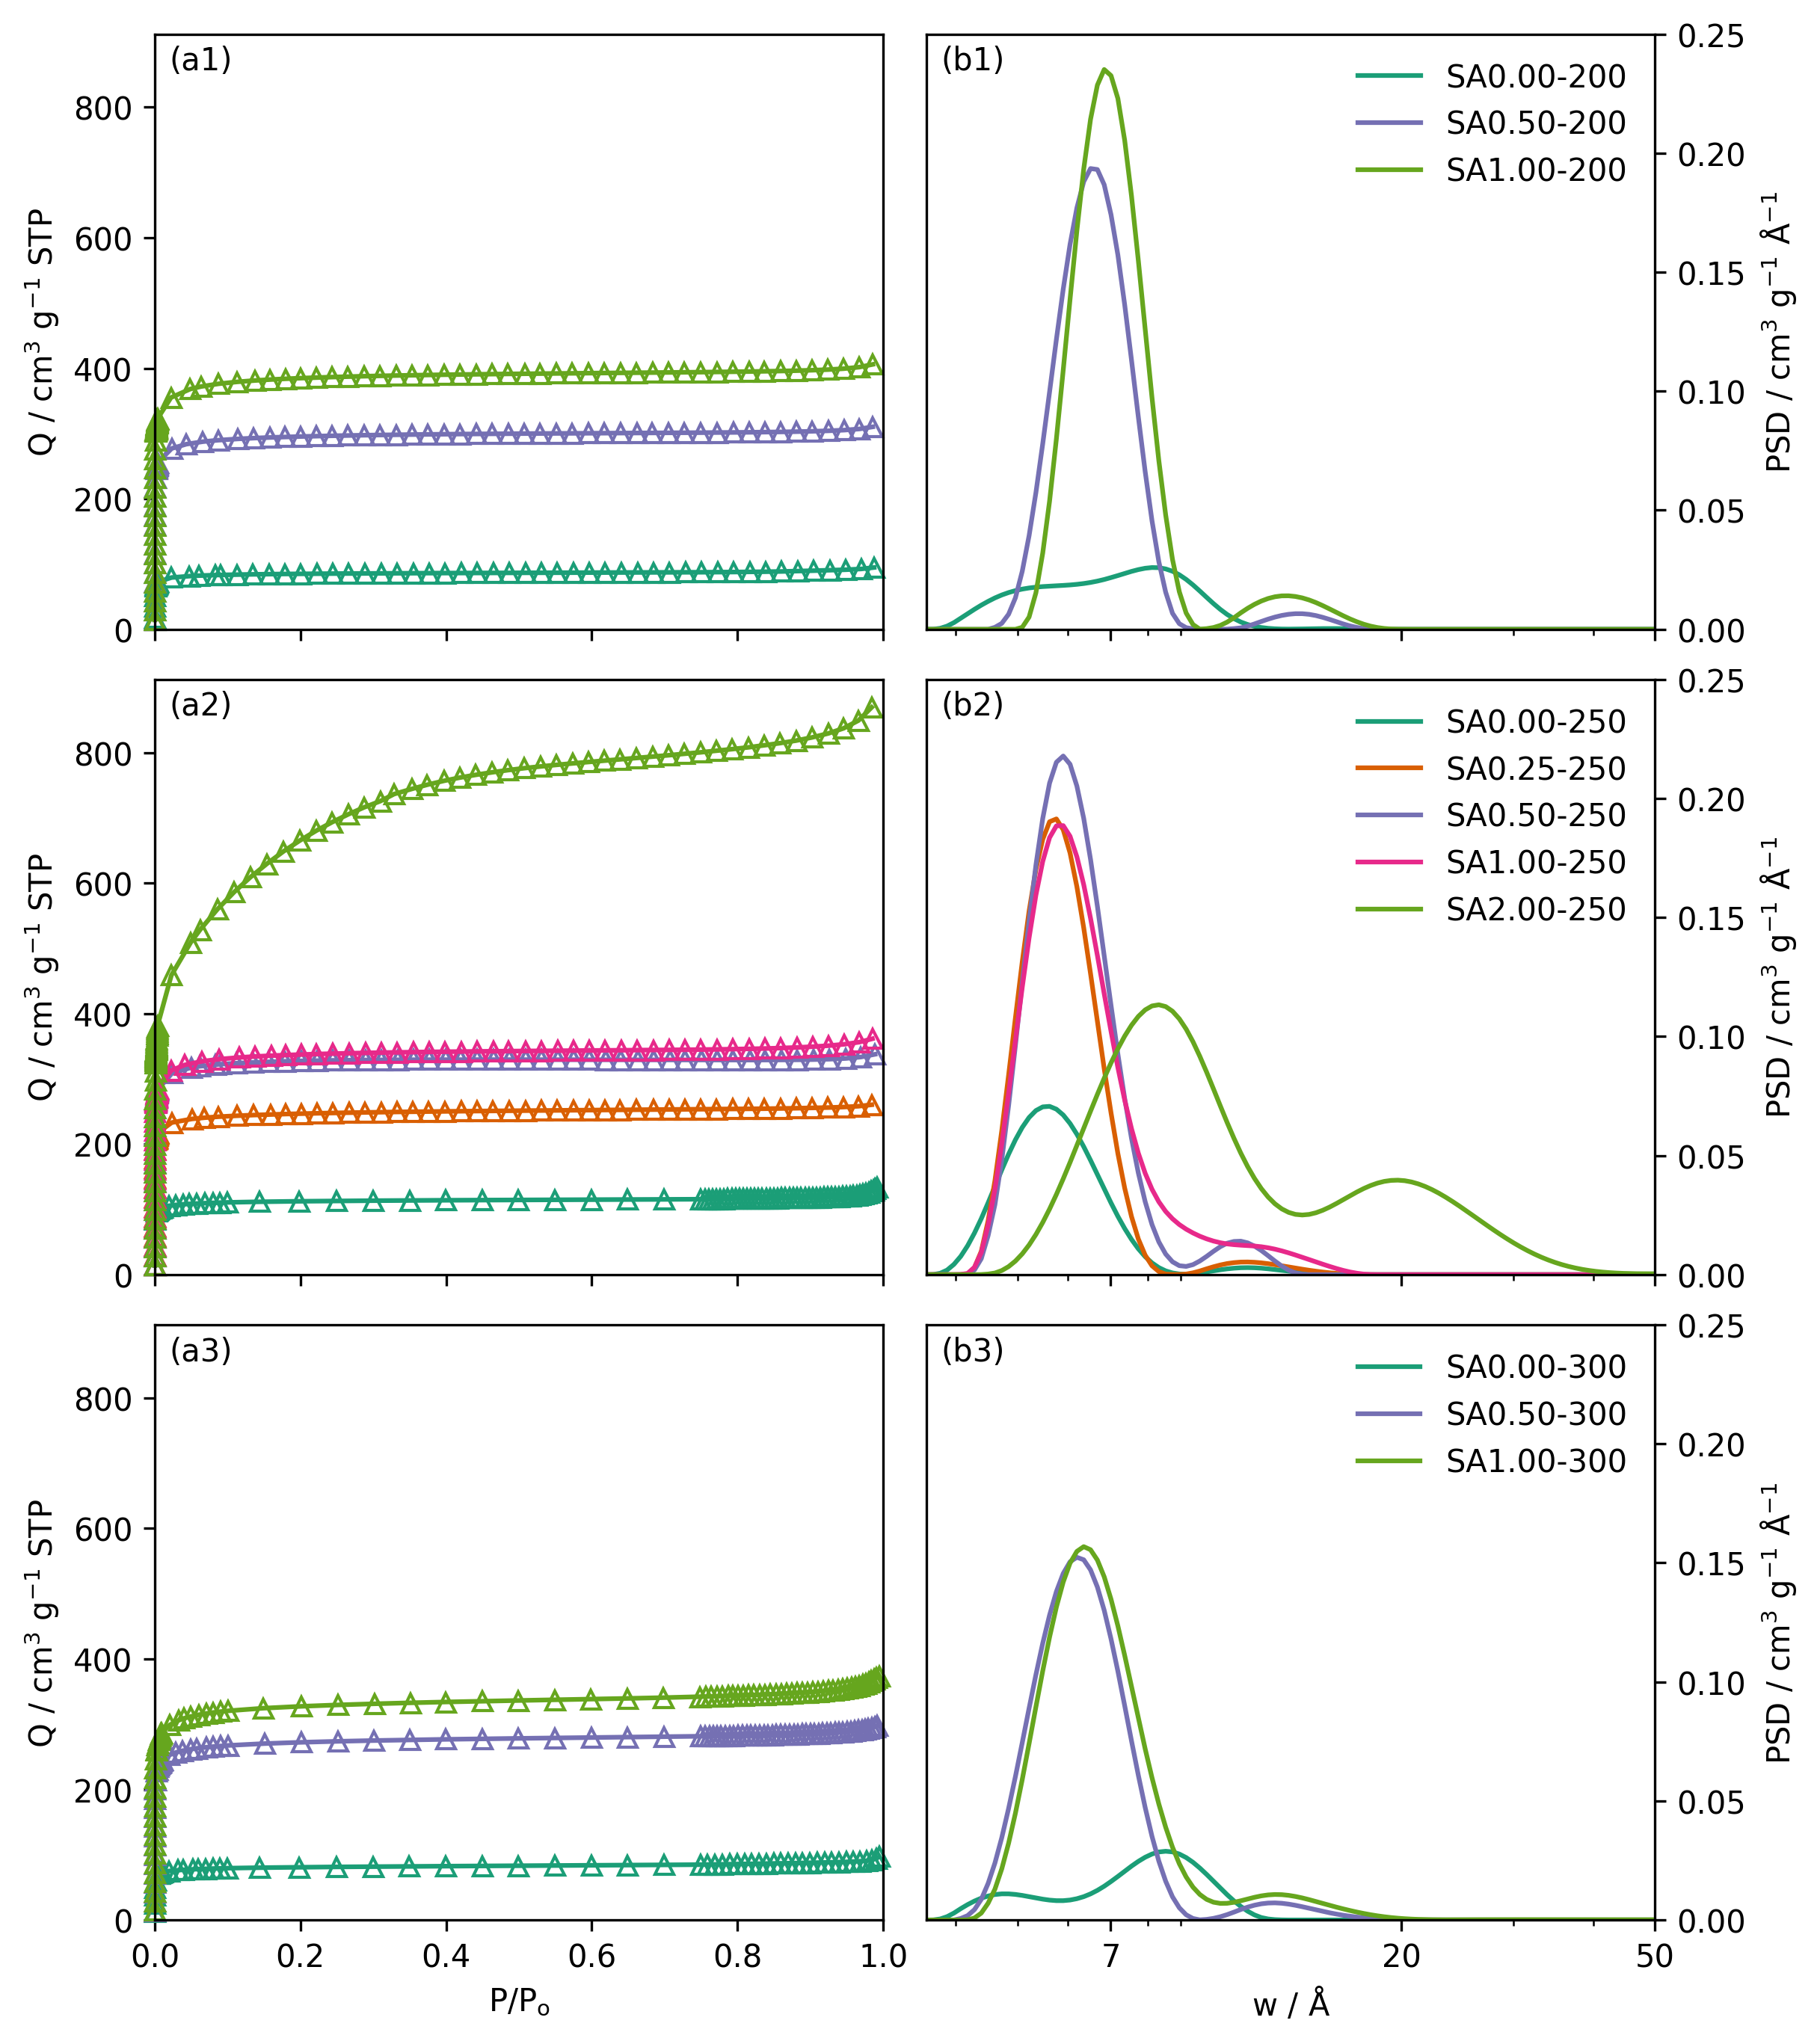
\includegraphics[width=\columnwidth, keepaspectratio]{4-impregnation/figs/SA_n2_isotherms.png}
    \caption{Isotherms (column a) and resultant \acrshortpl{psd} (column b) for SA samples hydrothermally carbonised at \qtylist[list-units=single]{200;250;300}{\degreeCelsius} (rows 1, 2 and 3 respectively).}
    \label{fig:SA_n2_isotherms}
\end{figure}

In the case of SA0.00-\textit{HHH} samples, overall surface area and pore volume (\qty{456}{\metre\squared\per\gram} and \qty{0.18}{\cm\cubed\per\gram}) was maximised where the \gls{htc} temperature was \qty{250}{\degreeCelsius}. Increasing \gls{htc} temperature generally reduces \ce{C} content in the resultant \gls{hydrochar},\citep{Sevilla2009a, parshetti2013chemical, kim2014hydrothermal} however temperatures above \qty{250}{\degreeCelsius} have also been shown to result in the break down of the poylmerised product into volatile organic moieties.\citep{gao2012characterization, Xiao2012Hydrothermal, wang2018review} As such, the apparent optimisation of porosity found by preparation with \gls{htc} at \qty{250}{\degreeCelsius} is likely a result of both of these factors affecting the activation resistance\citep{Altwala2020Predictable, Blankenship2022Modulating} and thus ultimately the porosity of the resultant activated carbon.

As for the \ce{KOH}-activated samples, in general increasing \ce{KOH}:\acrshort{sd} ratio is associated with increases in overall porosity, with SA2.00-250 achieving the highest surface area and pore volume of \qty{2396}{\metre\squared\per\gram} and \qty{0.84}{\cm\cubed\per\gram} respectively. In general this improvement does not appear to significantly effect microporosity which remains in the range \numrange[range-phrase={-}]{88}{94} and \qtyrange[range-units=single, range-phrase={-}]{81}{92}{\percent} in terms of surface area and pore volume respectively. This is, until \ce{KOH}:\acrshort{sd} ratio is increased to \num{2.00}, wherein development of mesoporosity reduces percent micropore surface area to \qty{27}{\percent}. This is reflected in the \ce{N2} isotherm for this sample (see figure \ref{fig:SA_n2_isotherms}(a2)) which displays a large \gls{adsorption} knee, unlike the very pure type I isotherms\citep{Thommes2015Physisorption} of the remaining samples.

The additional KOH:\acrshort{sd} ratio of 0.25 and 2.00 were included at \gls{htc} temperature of \qty{250}{\degreeCelsius} due to the relative similarity of isotherms and resultant porosities where KOH:\acrshort{sd} ratio is 0.50 or 1.00. In all cases, percent microporosity remains approximately the same, and the pore size is identical at these two ratios (see table \ref{tb:sa_porosity}). There are of course small improvements in overall porosity (most pronounced according to pore volume), when the ratio is increased from 0.50 to 1.00, but not to the extent that might be expected for a doubling of the amount of \gls{porogen} in the reaction mixture. This is most evident when examining differential \glspl{psd} (see figure \ref{fig:SA_n2_isotherms}(b1-3)) where for all SA\textit{x.xx-HHH} samples with \textit{x.xx} between 0.25 and 1.00 the profile is essentially the same, with porosity centered at \qtyrange[range-units=single, range-phrase={-}]{6}{8}{\angstrom}, and having minor shifts in position and/or size of the maximum which may simply be attributable to fitting of the kernel to the at times poorly equilibrated isotherm (see appendix, figures \ref{fig:SAxxx-200_isopsd}-\ref{fig:SAxxx-300_isopsd}). Similarly, for samples wherein \textit{x.xx} is 0.00, the \gls{psd} is much broader with low porosity at any given value of $w$, but all porosity remains in the \gls{micropore} region. Conversely, SA2.00-250 displays a clear hierarchical \gls{psd} with significant porosity in both the \gls{micropore} and small \gls{mesopore} range. 


In their 2017 work Balahmar \textit{et al.} report carbons which were synthesised by activation with \ce{KOH}  activation at \qty{800}{\degreeCelsius} either of untreated sawdust or sawdust-derived \gls{hydrochar} synthesised at \qty{250}{\degreeCelsius}.\citep{Balahmar2017Biomass} Figure \ref{fig:SA_porosity_compare} compares these results. $A_{BET}$ is compared in terms of both \ce{KOH}:precursor mass ratio, and atomic \ce{K}:\ce{C} ratio; the latter according to the elemental composition of the precursor (sawdust or \gls{hydrochar}). The three methods, i.e. direct activation of sawdust, activation of \gls{hydrochar}, and hydrothermal impregnation of \ce{KOH} into sawdust do not seem to show any significant difference in terms of the overall $A_{BET}$ of the final product. Indeed, there is a clear strong linear correlation  between amount of \ce{KOH} used and $A_{BET}$; $r^2=0.90$, regardless of whether mass of \ce{KOH} or amount of \ce{K} is considered. The slopes of the linear regressions on figure \ref{fig:SA_porosity_compare}(a1, a2) are \qtylist[list-units=single]{523;386}{\metre\squared\per\gram}, respectively. Thus, increases in $A_{BET}$ with increasing amount of \ce{KOH} can be precisely predicted. Furthermore, the temperature used in the hydrothermal impregnation step (this work) does not significantly effect $A_{BET}$ of the final product. However, the microporosity of the product is significantly effected by synthetic method. At a \ce{KOH}:precursor mass ratio of 2.00, microporosity is maximised by direct activation of sawdust at \qty{84}{\percent}, which decreases to \qty{63}{\percent} for activation of sawdust-derived \gls{hydrochar}, and finally to \qty{27}{\percent} for the hydrothermal impregnation method. These results are also reflected by the very broad, principally mesoporous \gls{psd} of SA2.00-250 relative to the comparable samples reported in the paper by Balahmar and co-workers.\citep{Balahmar2017Biomass} 

\begin{figure}[t!]
    \centering
    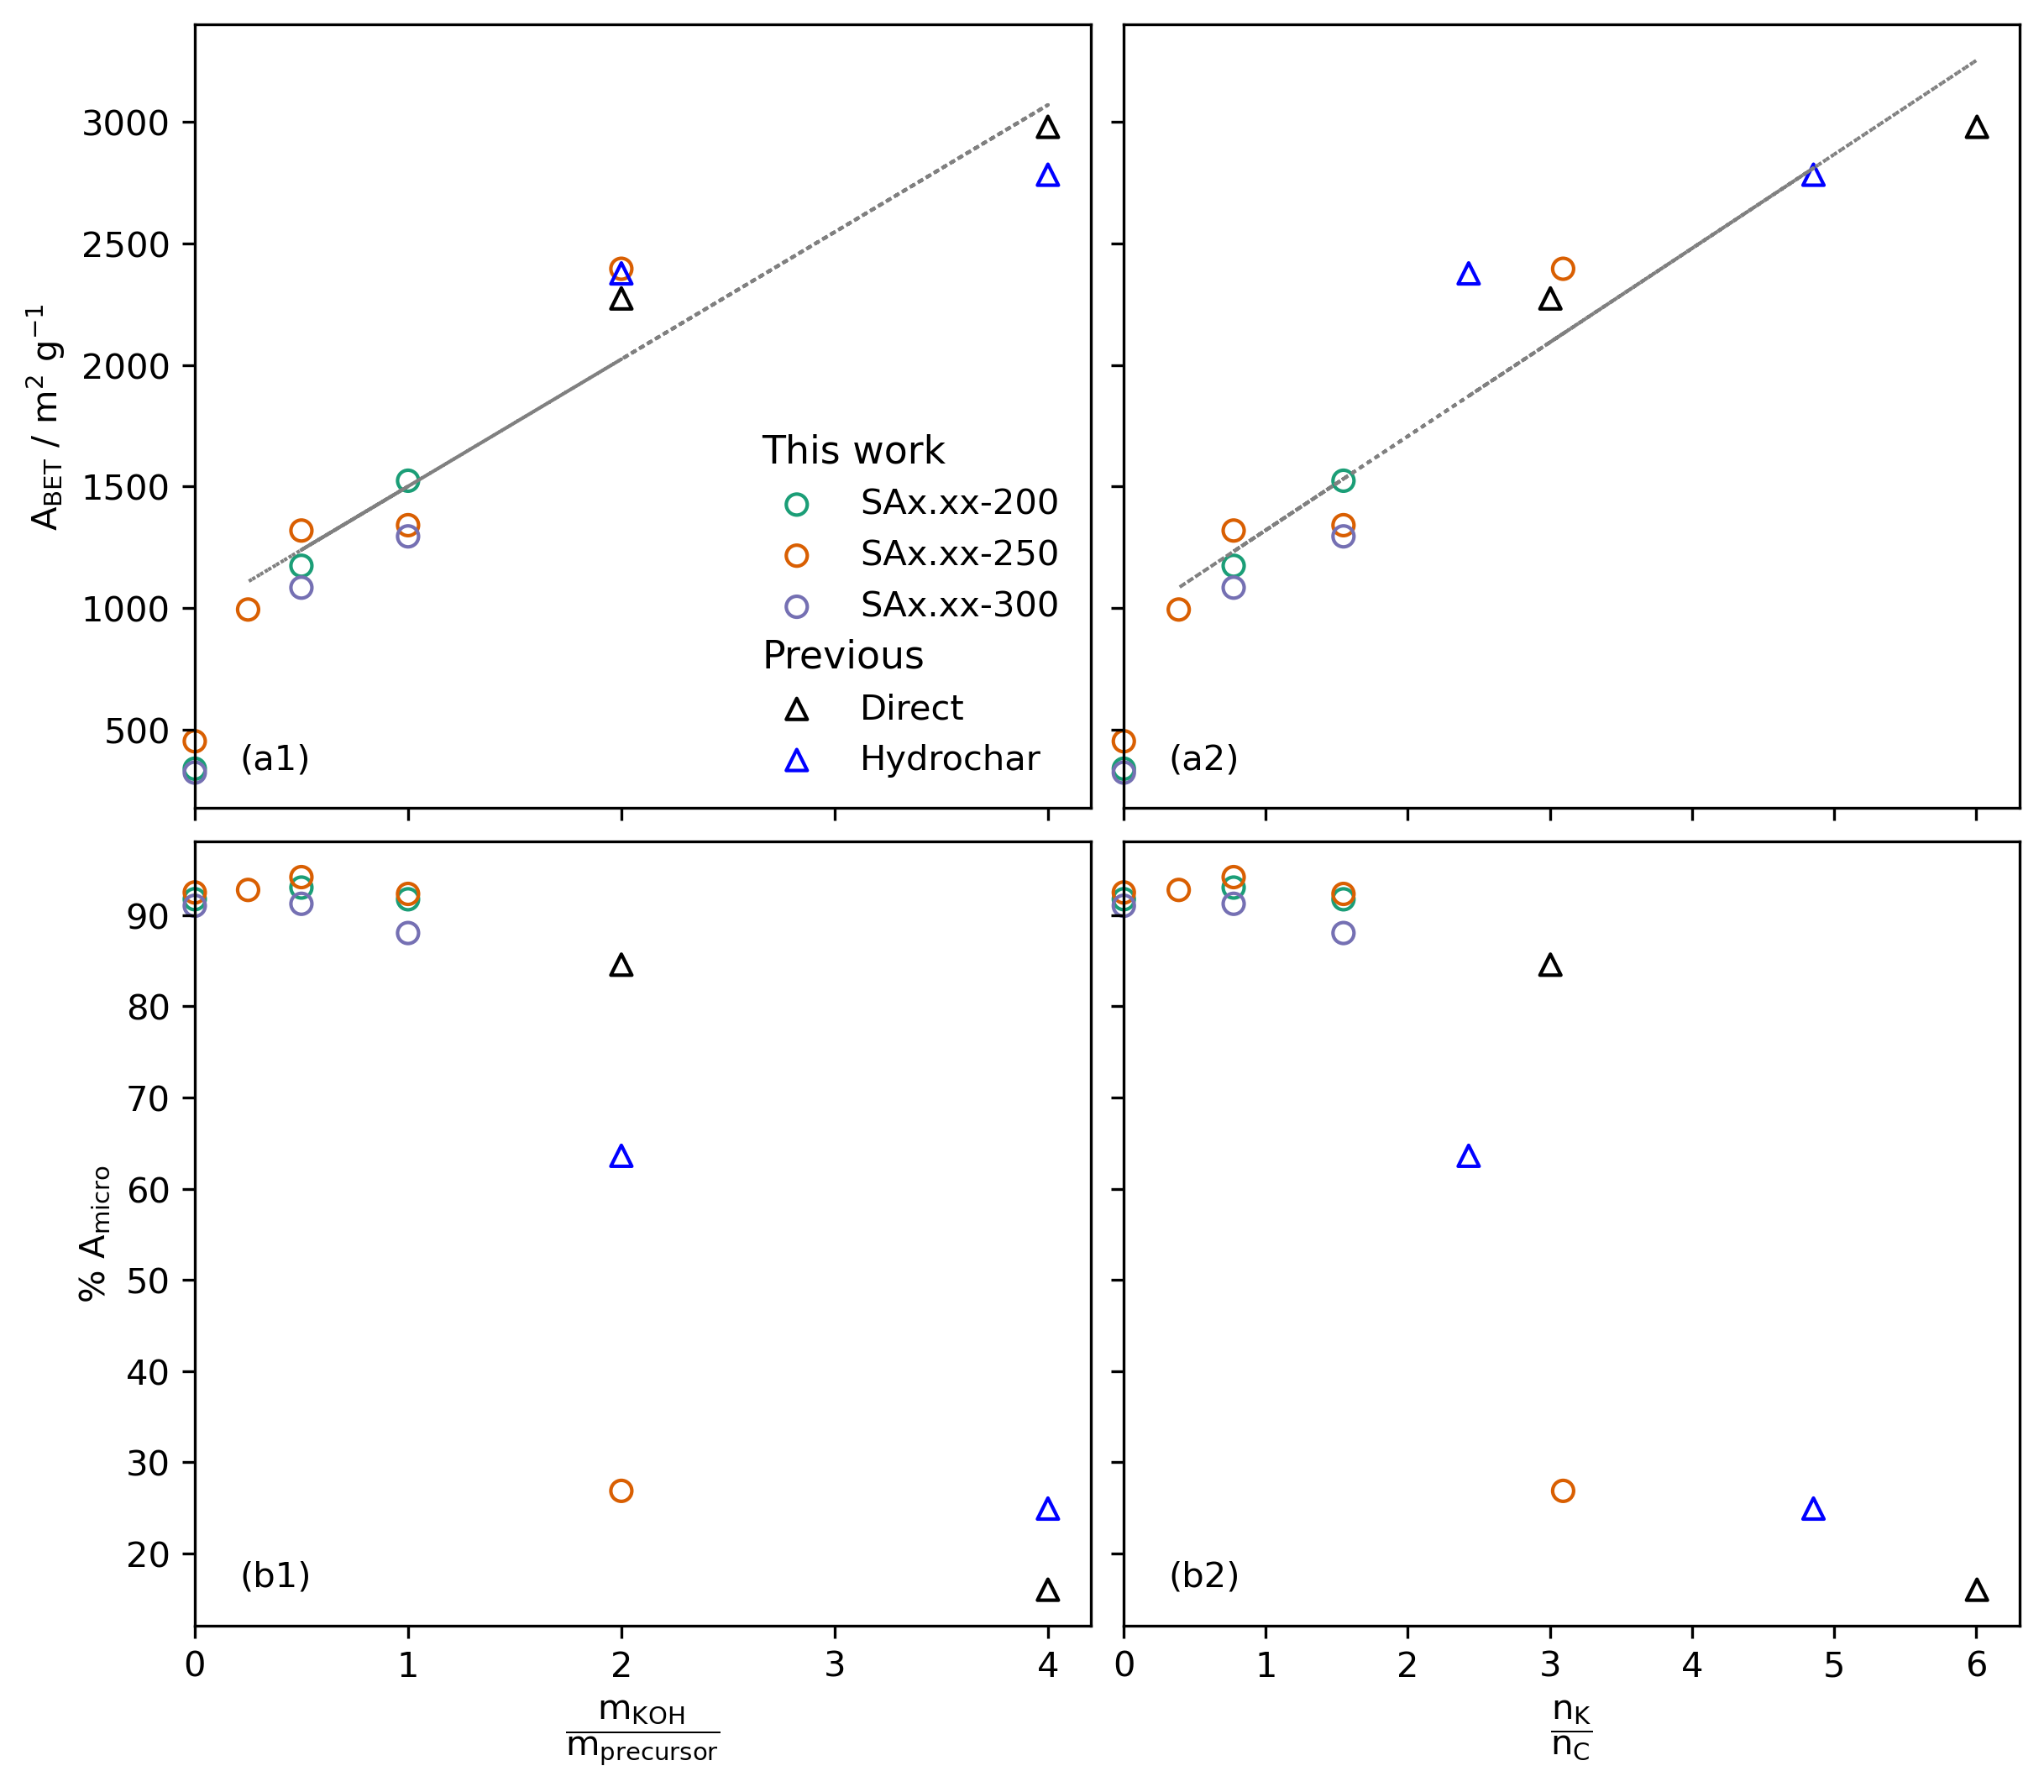
\includegraphics[width=\columnwidth, keepaspectratio]{4-impregnation/figs/SD_porosity_compare.png}
    \caption{Relationship between amount of \ce{KOH} used in activation of sawdust and porosity. Samples synthesised by Balahmar \textit{et al.} included to show effect of different methods of preparation.\citep{Balahmar2017Biomass} Amount of \ce{KOH} shown as KOH:precursor mass ratio (column 1), and as \ce{K}:\ce{C} atomic ratio (column 2). Porosity shown in terms of total $A_{BET}$ (row a) and micropore surface area calculated using t-plot (row b).}
    \label{fig:SA_porosity_compare}
\end{figure}

\paragraph{Density}

\begin{figure}[ht!]
    \centering
    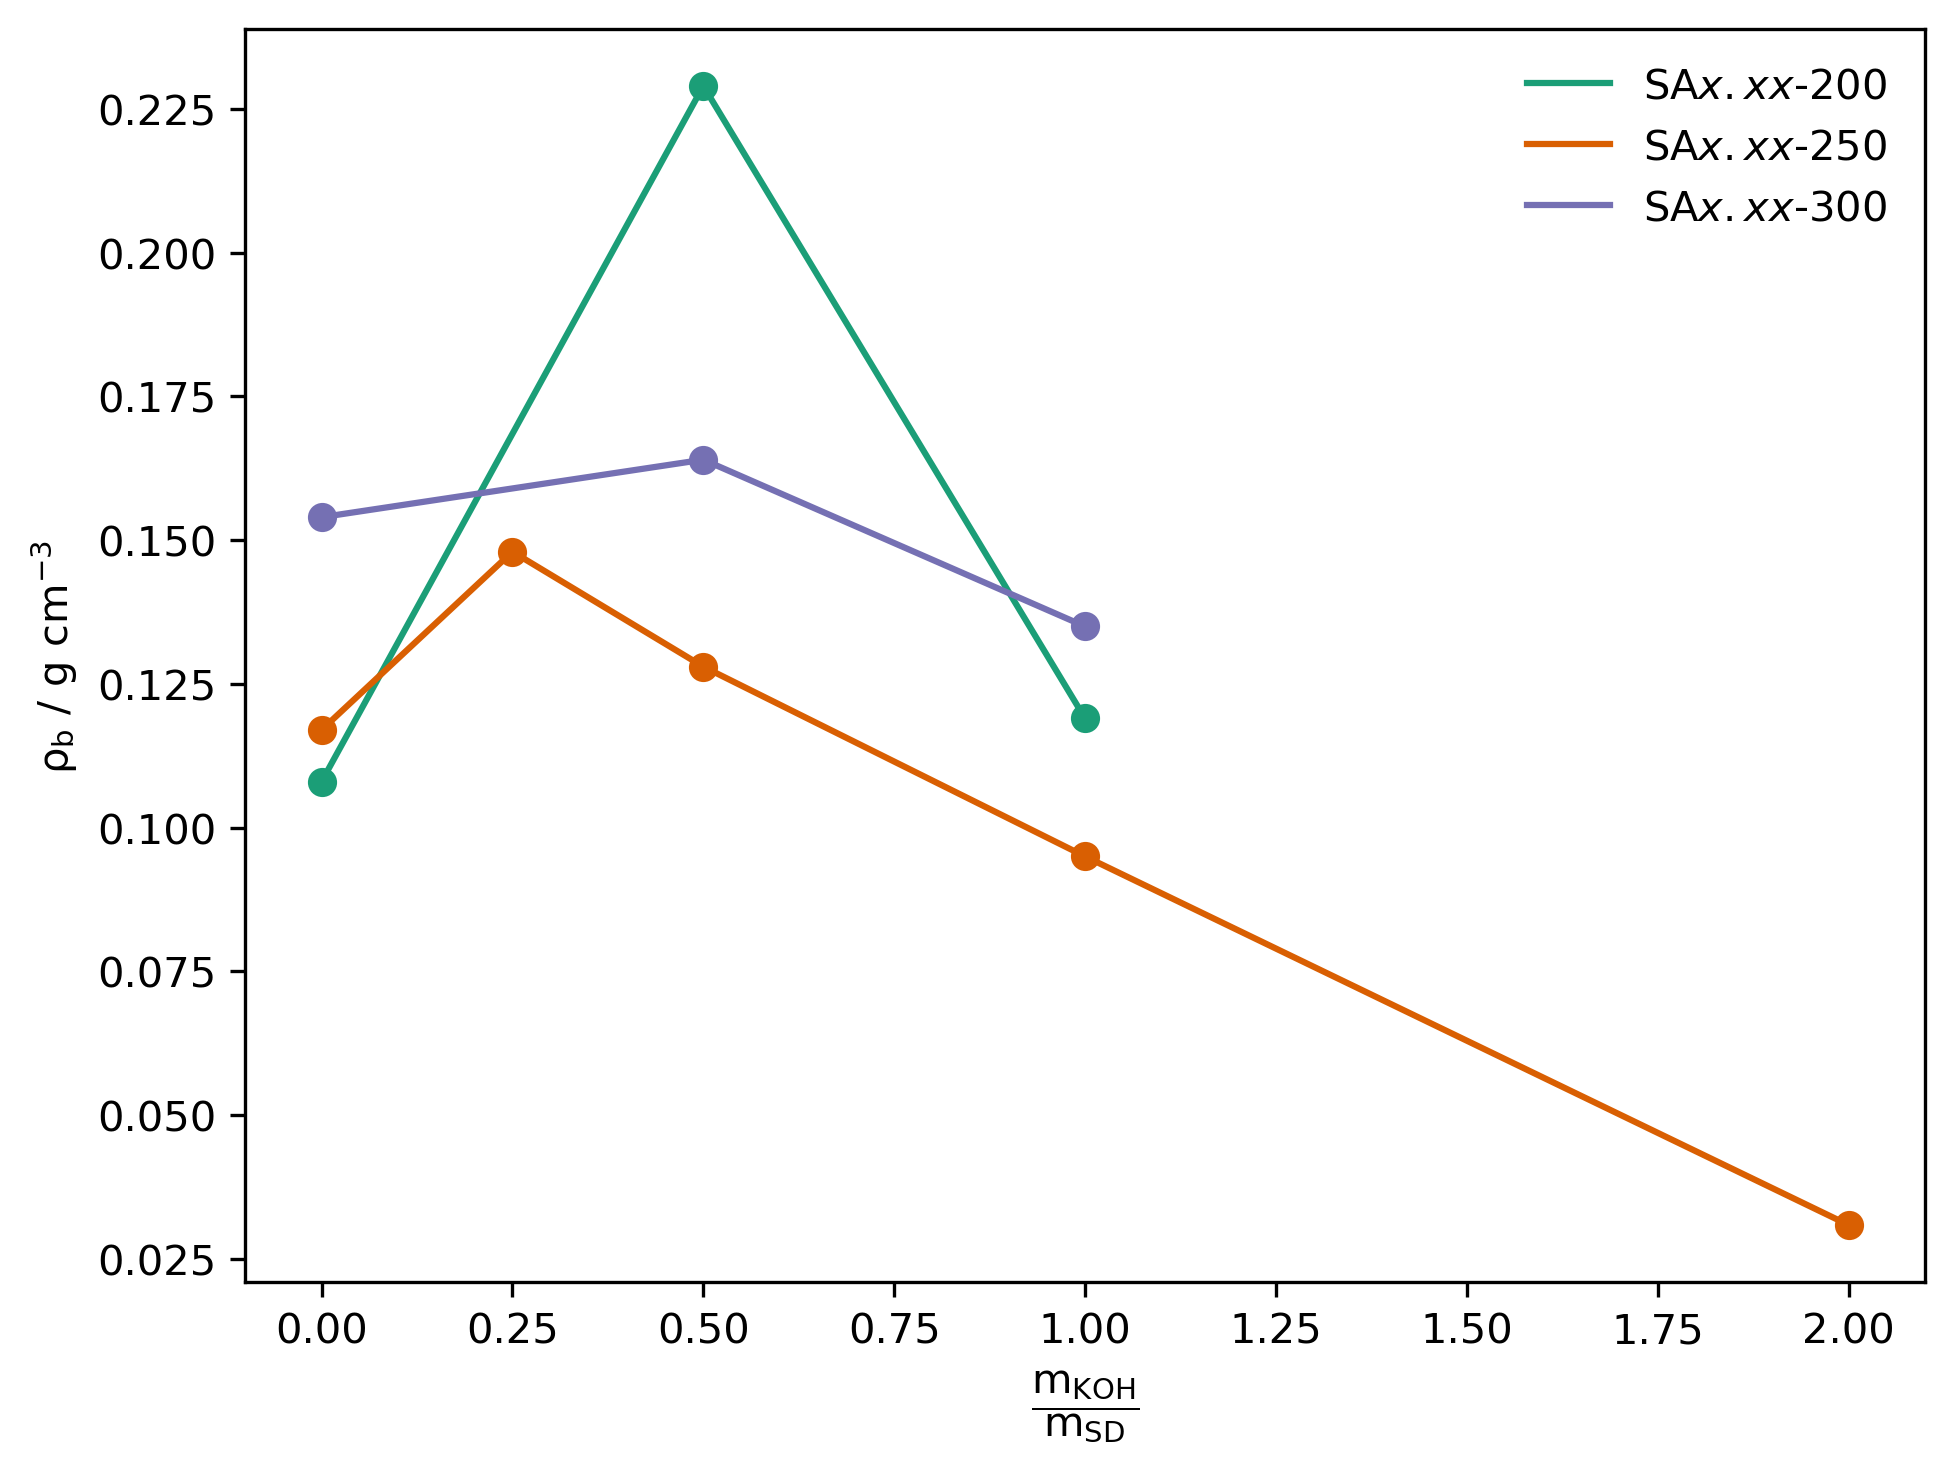
\includegraphics[width=\columnwidth, keepaspectratio]{4-impregnation/figs/SD_density.png}
    \caption{Effect of \ce{KOH}:\acrshort{sd} ratio on bulk density, $\rho_b$ of carbons synthesised using the three \ce{htc} temperatures. $\rho_b$ estimated from freespace measurements.}
    \label{fig:SA_density}
\end{figure}

As mentioned in subsection \ref{ss:sd_results}, sample SA2.00-250 was noticeably more diffuse than the other samples. In lieu of access to appropriate pycnometric equipment, bulk density ($\rho_{b}$) of samples found here was estimated by using ambient temperature \ce{He} freespace measurements during the measurement of \ce{N2} isotherms. The sample volume was taken as the difference between this freespace and the ambient freespace of the empty tube, thus calculation of the $\rho_{b}$ was trivial as sample mass is already known. These estimated bulk densities are shown in figure \ref{fig:SA_density}. Densities of these carbons are at the low end of that  reported for \ce{KOH}-activated carbons,\citep{casco2015very, machnikowski2012adsorption, Altwala2020Predictable} however similar values have been reported by some groups.\citep{tseng2008effects, rashid2016koh, Guan2011Methane} Additionally, for \ce{KOH} activated samples, $\rho_b$ is negatively correlated with amount of \ce{KOH} used during activation, similarly to reports by Tseng \textit{et al.}.\citep{tseng2008effects} The extremely low bulk density (\qty{0.031}{\gram\per\cm\cubed}) of SA2.00-250 may be ascribed to an effect described by Deng and co-workers in 2015, i.e. that high production of gases by the activating agent results in bulk densities as low as \qty{0.043}{\gram\per\cm\cubed} and hierarchical \glspl{psd}.\citep{Deng2015Inspired} While the gas production in the work by Deng \textit{et al.} is thought to be a result of decomposition of the \ce{KHCO3} \gls{porogen}, in this study reactions of excess aqueous \ce{KOH} with the precursor during the hydrothermal impregnation step may form \glspl{porogen} that have a similar capacity to release gases such as \ce{CO2}. This does not however serve to explain the low densities of the remaining samples which are almost exclusively microporous. 

\newpage
\subsection{Sodium Carboxymethyl Cellulose}
\label{ss:NC}

Twelve carbon samples were produced from sodium carboxymethyl cellulose with varying \acrshort{ds}. On removal from the furnace, samples derived from precursors containing \ce{Na} glowed red due to exposure of small amounts of elemental \ce{Na} to air, thus indicating this specie is a product of the activation process. While there is some debate as to whether elemental metals form during activation with \ce{KOH} or \ce{NaOH},\citep{Blankenship2022Modulating, Sevilla2014Energy, LozanoCastello2007Carbon, Kelemen1983interaction, Xue2003Formation} it is clear that it occurs here. In addition, these samples took the form of a single, hard mass whereas activated carbons are typically powders. On washing with \ce{HCl}, the samples broke up into a fine powder. This indicates that residual \ce{Na} compounds or other by-products of activation may be holding particles together in some way.

\subsubsection{Composition}
\label{sss:NC_composition}

\begin{figure}[htpb!]
    \centering
    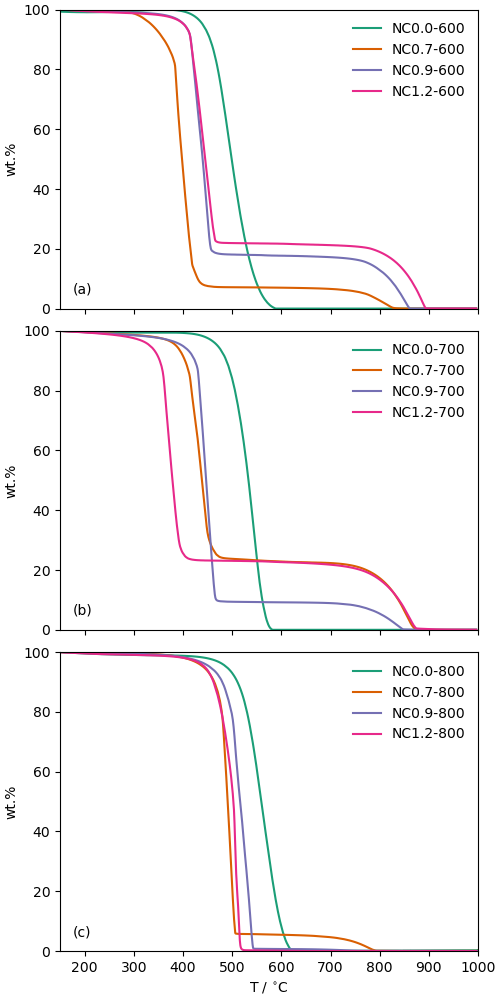
\includegraphics[width=0.82\columnwidth, keepaspectratio]{4-impregnation/figs/NC_tga_adj.png}
    \caption{\acrshort{tga} curves for all NC\textit{x.x-TTT} samples, adjusted for water evaporation, and residual masses set to 0, where within \qty{1}{\wtpercent}. Original (unadjusted) thermograms are provided in figure \ref{fig:NC_tga}.}
    \label{fig:NC_tga_adj}
\end{figure}

\acrshort{tga} (shown in figure \ref{fig:NC_tga_adj}) of the twelve samples confirms that the washing process removed any residual \ce{Na} compounds, i.e. the samples are all fully carbonaceous. In order to simplify direct comparisons between the combustion behaviour of the samples, the initial mass loss (moisture loss) at \qty{100}{\degreeCelsius} is ignored, and initial mass is taken to be that of the dry sample. In addition, the residual mass has been adjusted to \qty{0}{\wtpercent} for all samples to improve plot readability.\footnote{Unadjusted \acrshort{tga} curves can be found in the appendix, figure \ref{fig:NC_tga}.} For some of the \glspl{turbostratic carbon} there is a large loss of mass at between \qtylist[list-units=single]{400;500}{\degreeCelsius}, before the remainder of the sample is burned off. This is followed by a second burn-off event between \qtylist[list-units=single]{800;900}{\degreeCelsius}. In the case of samples with only a single burn-off temperature, this occurs at between \qtylist[list-units=single]{500;650}{\degreeCelsius}. The dual burn-offs appear to be associated with the presence of \ce{Na} in the precursor, as all NC0.0-\textit{TTT} samples only display a single-burn off. Furthermore, both the amount of \ce{Na} in the precursor and the activation temperature influence the temperature and mass decrease in the first mass loss (when it is present). For example, for NC\textit{x.x}-600 samples, the mass loss associated with the initial burn-off decreases with increasing \acrshort{ds}, while the temperature of this process increases. The trend for NC\textit{x.x}-700 is more convoluted, and for NC\textit{x.x}-800 samples only NC0.7-800 displays the dual burn-off behaviour. Nonetheless, it appears that the oxidative \gls{porogen} (here in the form of \ce{Na} and/or \ce{CH2COONa} and/or other various derivatives) produces two phases in the resultant carbons to varying extents depending on the activation temperature and \ce{Na}:\ce{C} ratio. 

\begin{figure}[hptb]
    \centering
    \captionof{table}{Composition of sodium carboxymethyl cellulose at all values of \acrshort{ds}, and of NC\textit{x.x-TTT} carbons according to CHN elemental microanalysis. For NC\textit{x.x-TTT} carbons, \ce{O} content is taken as remainder of the sum of \ce{C} and \ce{H} contents as samples are clean according to \acrshort{tga}. \ce{N} content not shown as it is zero for all samples.}
    \label{tb:nc_chn}
    \begin{tabularx}{0.9\textwidth}{lXXXXXXX}
    \toprule
        \textbf{Sample} & \multicolumn{4}{c}{\textbf{Concentration / \unit{\wtpercent}}} & \multicolumn{3}{c}{\textbf{Atomic ratio}} \\
        & \textbf{C} & \textbf{H} & \textbf{O} & \textbf{Na} & \textbf{O/C} & \textbf{H/C} & \textbf{Na/C} \\
    \midrule
        \textbf{NC0.0} & 44 & 6.2 & 49 & 0 & 0.83 & 0.14 & - \\
        \textbf{NC0.0-600} & 87 & 1.9 & 11 & 0 & 0.10 & 0.26 & - \\
        \textbf{NC0.0-700} & 91 & 0.97 & 8.5 & 0 & 0.07 & 0.13 & - \\
        \textbf{NC0.0-800} & 92 & 0.46 & 7.4 & 0 & 0.06 & 0.06 & - \\
        \\
        \textbf{NC0.7} & 41 & 5.2 & 47 & 7.4 & 0.87 & 0.13 & 0.09 \\
        \textbf{NC0.7-600} & 76 & 2.8 & 21 & 0 & 0.21 & 0.43 & - \\
        \textbf{NC0.7-700} & 65 & 0.38 & 35 & 0 & 0.40 & 0.07 & - \\
        \textbf{NC0.7-800} & 85 & 0.37 & 15 & 0 & 0.13 & 0.05 & - \\
        \\
        \textbf{NC0.9} & 40 & 5.1 & 46 & 8.8 & 0.88 & 0.13 & 0.12 \\
        \textbf{NC0.9-600} & 83 & 0.26 & 17 & 0 & 0.16 & 0.04 & - \\
        \textbf{NC0.9-700} & 75 & 0.36 & 25 & 0 & 0.25 & 0.06 & - \\
        \textbf{NC0.9-800} & 90 & 0.3 & 9.5 & 0 & 0.08 & 0.03 & - \\
        \\
        \textbf{NC1.2} & 39 & 4.8 & 46 & 11 & 0.89 & 0.12 & 0.14 \\
        \textbf{NC1.2-600} & 66 & 0.89 & 33 & 0 & 0.38 & 0.16 & - \\
        \textbf{NC1.2-700} & 64 & 0.61 & 36 & 0 & 0.42 & 0.11 & - \\
        \textbf{NC1.2-800} & 76 & 0.06 & 24 & 0 & 0.24 & 0.01 & - \\
    \bottomrule
    \\
    \end{tabularx}

    \centering
    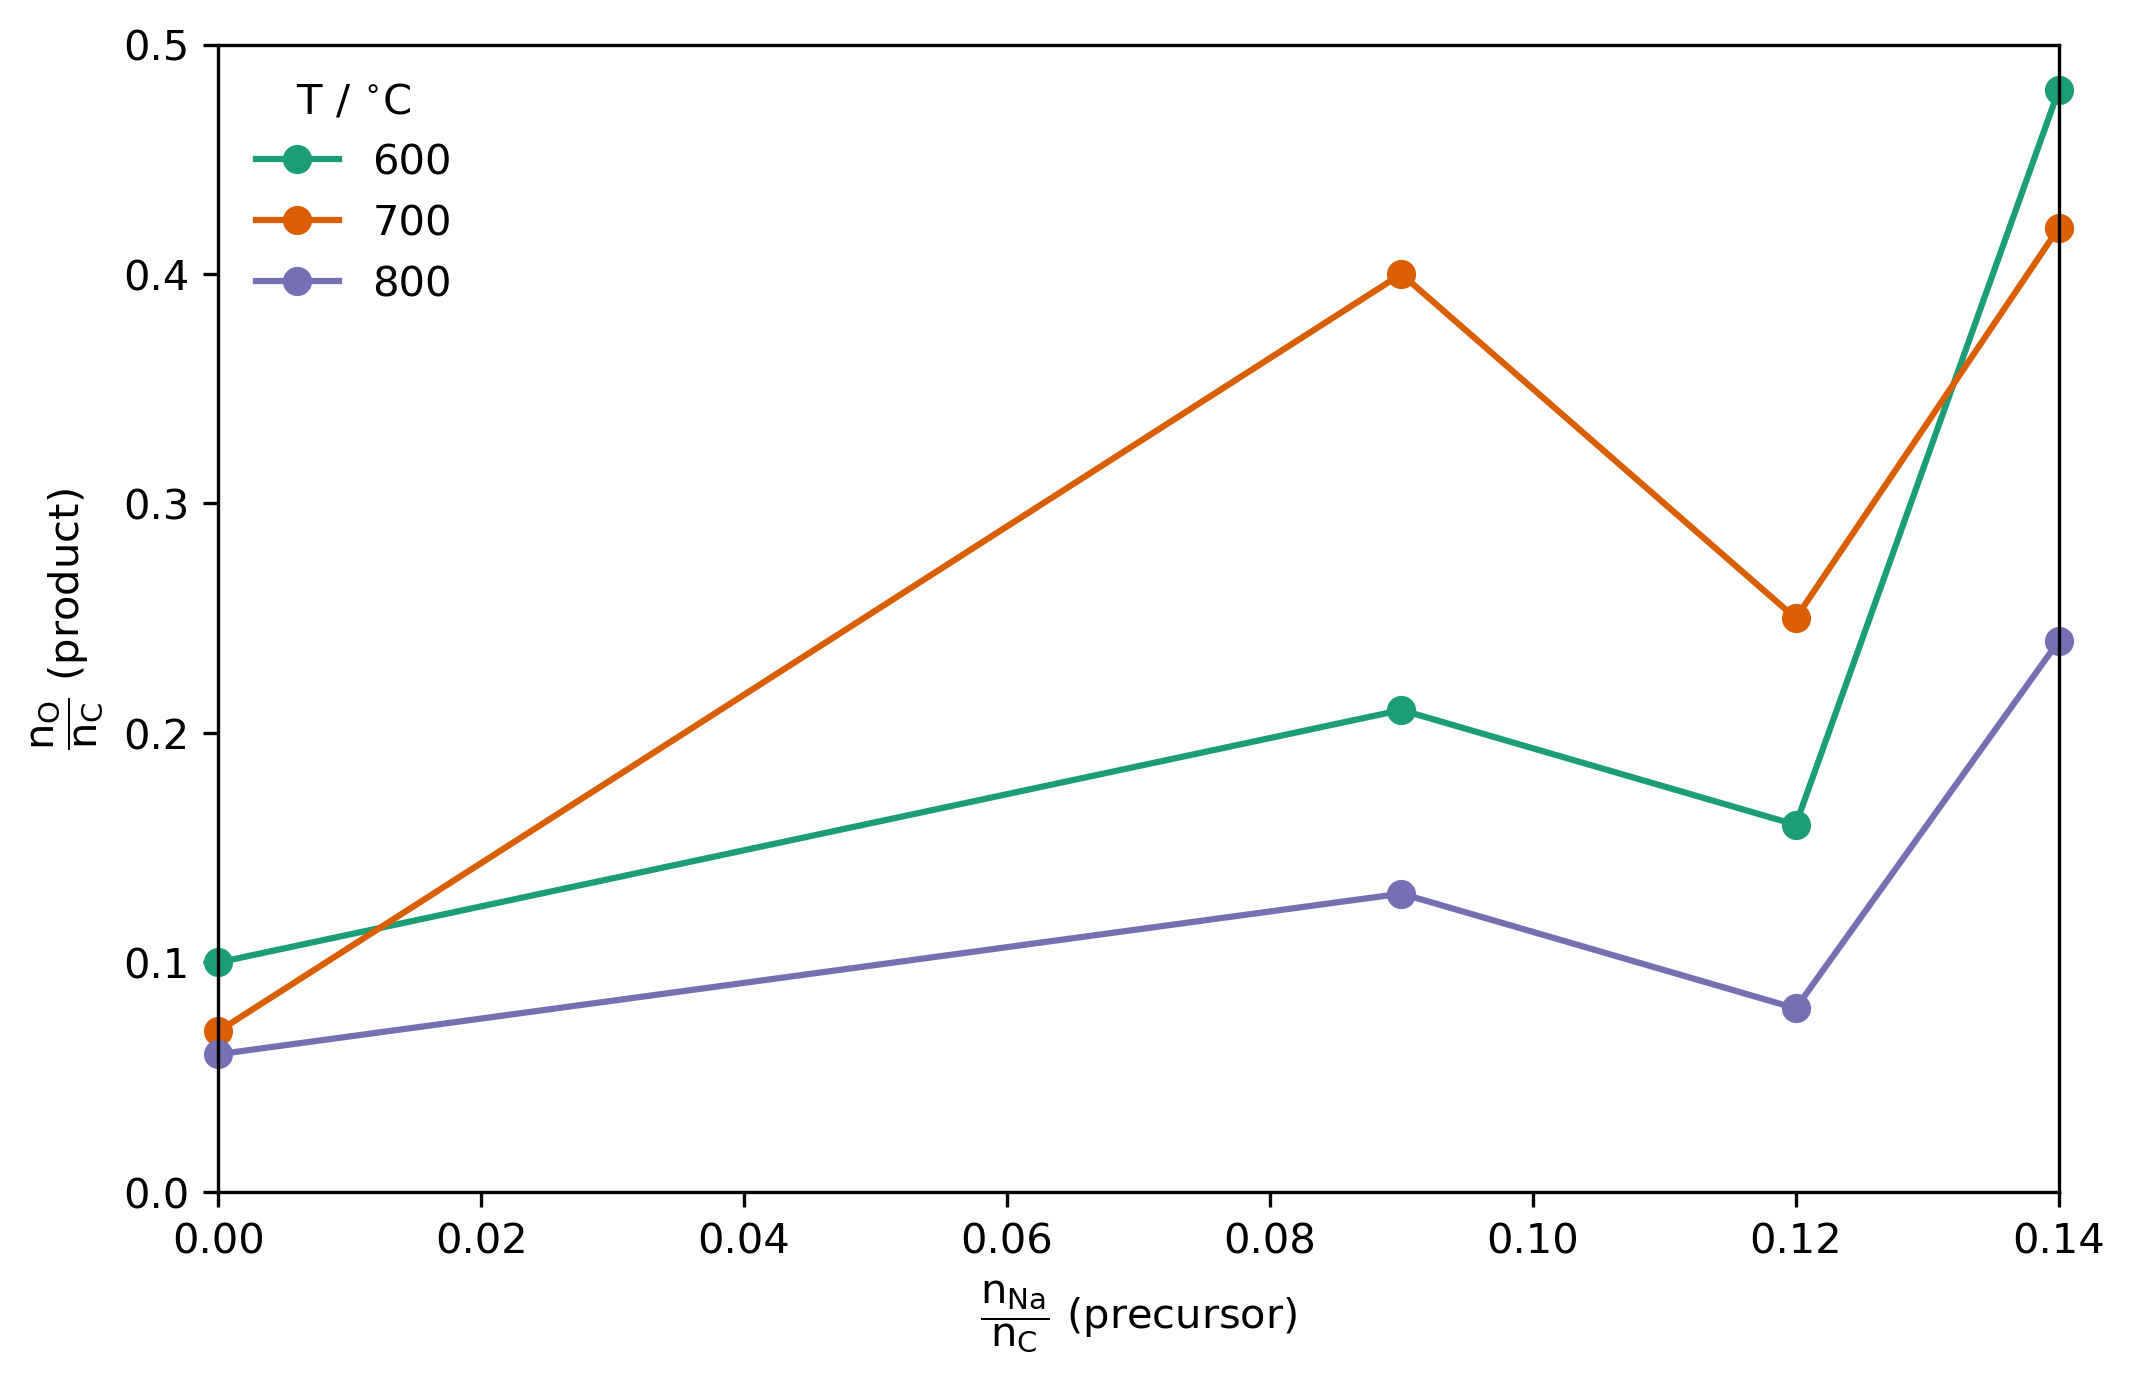
\includegraphics[width=\columnwidth, keepaspectratio]{4-impregnation/figs/NaCprecursor_OCproduct.png}
    \captionof{figure}{The effect of precursor \ce{Na}:\ce{C} ratio on the \ce{O}:\ce{C} ratio in the product at each of the three pyrolysis temperatures, $T$.}
    \label{fig:NaCprecursor_OCproduct}
\end{figure}

Results of CHN elemental microanalysis are shown in table \ref{tb:nc_chn}, alongside calculated concentrations of \ce{C}, \ce{H}, \ce{O}, and \ce{Na} in each of the four precursors. While there are variations in \ce{C}, \ce{H} and \ce{O} content between the four precursors, the most significant change is with respect to the \ce{Na}:\ce{C} ratio. The effect of precursor \ce{Na}:\ce{C} ratio on product \ce{O}:\ce{C} ratio is shown in figure \ref{fig:NaCprecursor_OCproduct}. Typically, increased oxidative \gls{porogen} concentration results in higher relative \ce{O} contents in the derived porous carbon, commonly believed to be due to increased destruction of the \ce{C} framework.\citep{park2002effect, chen2020insight, tseng2007physical} What is interesting in the case of these sodium carboxymethyl cellulose-derived carbons is that there is a consistent minimum in atomic \ce{O}:\ce{C} ratio for carbons derived from precursors with a \ce{Na}:\ce{C} of 0.12, i.e. a \acrshort{ds} of 0.9, regardless of activation temperature. The effect of quantity of \gls{porogen} on the mechanism of oxidative chemical activation is not typically investigated for such low \gls{porogen}:\ce{C} ratios, so there is little to base a mechanistic hypothesis on for this case. However, it is possible that there is a balance being struck between formation of cross-links and activation with the \ce{Na+} cation (or its derivatives). Cross-link formation, if it occurs ought to result in the loss of \ce{O} due to the condensation of the two carboxylate groups to form the anyhdride linkage. Thus the drop in the \ce{O} concentration at a \acrshort{ds} of 0.9 may indicate the dominance of the (\ce{O}-removing) cross-linking process over the (\ce{O}-increasing) oxidative action of the \gls{porogen}. Similarly, the high \ce{O} content of samples synthesised at \qty{700}{\degreeCelsius} relative to the other two temperatures may be a function of the two competitive mechanisms. That is, pyrolysis at \qty{700}{\degreeCelsius} is optimal for cross-link formation. It should be noted however, that cross-linkages between sodium carboxymethyl cellulose chains have thus far only been shown to form as a result of low temperature, solution phase reactions with the use of reagents to promote their formation.\citep{lin2015preparation, yu2017koh, yu2017one}

\subsubsection{Porosity}

The samples in this work were not expected to have a high degree of porosity, and thus not expected to be particularly suitable candidates for gas sorption applications. Classical measures of porosity of the twelve carbons are displayed in table \ref{tb:nc_porosity}, and the \ce{N2} isotherms from which these quantities are derived as well as the resultant \acrshort{psd}s are shown in figure \ref{fig:NC_n2_isotherms}. Full details of \acrshort{psd}s and fitting to \acrshort{nldft} kernels are shown in the appendix, figures \ref{fig:NCxx-600_psdisofull}-\ref{fig:NCxx-800_psdisofull}.\footnote{Due to poor equilibration, these \acrshortpl{psd} cannot be considered to be accurate, this is discussed in more depth in chapter \ref{ch:dual_isotherm} and \ref{pub:dual_iso}.} Most samples are highly microporous according to t-plot calculations, having 87-91 \% and 75-90 \% \gls{micropore} surface area and pore volume respectively. The notable exceptions to this are NC0.7-600 wherein $A_{BET}$ and $V_t$ are so low that t-plot calculations are rendered extremely imprecise, as well as NC1.2-600 and NC1.2-800. The slightly lower microporosity of the latter two samples may be attributed to increased \gls{mesopore} development due to higher quantities of \gls{porogen}. 

\begin{table}[ht!]
    \caption{Porosity of NC\textit{x.x-TTT} carbons. $A_{BET}$ derived using the Rouquerol method. The total pore volume, $V_t$ is taken using the single point method. Values in brackets indicate the microporous portion of $A_{BET}$ and $V_t$, calculated using t-plot. Peak pore width $w_{peak}$ is the maximum of the \acrshort{psd} determined using \acrshort{nldft}, as shown in figure \ref{fig:NC_n2_isotherms}.}
    \label{tb:nc_porosity}
    \begin{tabularx}{\textwidth}{Xllllll}
    \toprule
        \textbf{Sample} & \multicolumn{2}{l}{$\mathbf{A_{BET}}$ \textbf{/ \unit[detect-weight]{\metre\squared\per\gram}}}  & \multicolumn{2}{l}{$\mathbf{V_t}$ \textbf{/ \unit[detect-weight]{\cm\cubed\per\gram}}} & \multicolumn{2}{l}{$\mathbf{w_{peak}}$ \textbf{/ \unit{\angstrom}}} \\
    \midrule
        \textbf{NC0.0-600} & 587 & (530) & 0.24 & (0.21) & 6 \\
        \textbf{NC0.7-600} & 21 & (13) & 0.01 & (-) & 7 \\
        \textbf{NC0.9-600} & 577 & (505) & 0.25 & (0.19) & 6 \\
        \textbf{NC1.2-600} & 238 & (213) & 0.10 & (0.08) & 6 \\
        \\
        \textbf{NC0.0-700} & 531 & (485) & 0.21 & (0.19) & 6 \\
        \textbf{NC0.7-700} & 162 & (151) & 0.07 & (0.06) & 7 \\
        \textbf{NC0.9-700} & 364 & (325) & 0.16 & (0.13) & 7 \\
        \textbf{NC1.2-700} & 190 & (169) & 0.08 & (0.06) & 5 \\
        \\
        \textbf{NC0.0-800} & 403 & (356) & 0.17 & (0.13) & 6 \\
        \textbf{NC0.7-800} & 491 & (427) & 0.21 & (0.16) & 6 \\
        \textbf{NC0.9-800} & 650 & (570) & 0.28 & (0.22) & 6 \\
        \textbf{NC1.2-800} & 476 & (382) & 0.21 & (0.15) & 5 \\
    \bottomrule
    \end{tabularx}
\end{table}

There are some clear trends with respect to overall porosity and both quantities of activating agent and activation temperature. The porosity of NC0.0-\textit{TTT} samples decreases with increasing activation temperature, while maintaining fairly constant microporosity (\qty{90(2)}{\percent}, by surface area), and average pore size of \qty{6}{\angstrom}. This indicates that for \glspl{biochar}, increasing activation temperature only serves to destroy porosity created at lower temperatures, while not broadening the \acrshort{psd} significantly. It has been previously observed that \gls{biochar} porosity is optimised with \gls{pyrolysis} temperature of around \qty{600}{\degreeCelsius},\citep{zama2017role, ronsse2013production, leng2021overview} although values for $A_{BET}$ and $V_t$ in these reports are around an order of magnitude less than shown by carbons reported herein from cellulose. Indeed, Zhang \textit{et al.} reported $A_{BET}$ and $V_t$ of only \qty{4.1}{\metre\squared\per\gram} and \qty{0.02}{\cm\cubed\per\gram} respectively for a carbon derived from the pyrolysis of cellulose at \qty{800}{\degreeCelsius},\citep{zhang2021pyrolysis} compared to the $A_{BET}$ of \qty{403}{\metre\squared\per\gram} for NC0.0-800. The samples reported here are more comparable in terms of porosity to that of the \gls{biochar} reported in chapter \ref{ch:cbs} derived from pure cellulose acetate (see table \ref{tb:CA_porosity}). This much higher surface area may simply be a result of washing of the biochars, which removes some soluble matter that contributed to pore blocking but may also be indicative of the low activation resistance of purely cellulosic materials relative to the traditionally carbonised ligno-cellulosic biomass.\citep{Hirst2018simple, Balahmar2019Pre, Zhang2019situ, Deng2016Effects} 

\begin{figure}[t!]
    \centering
    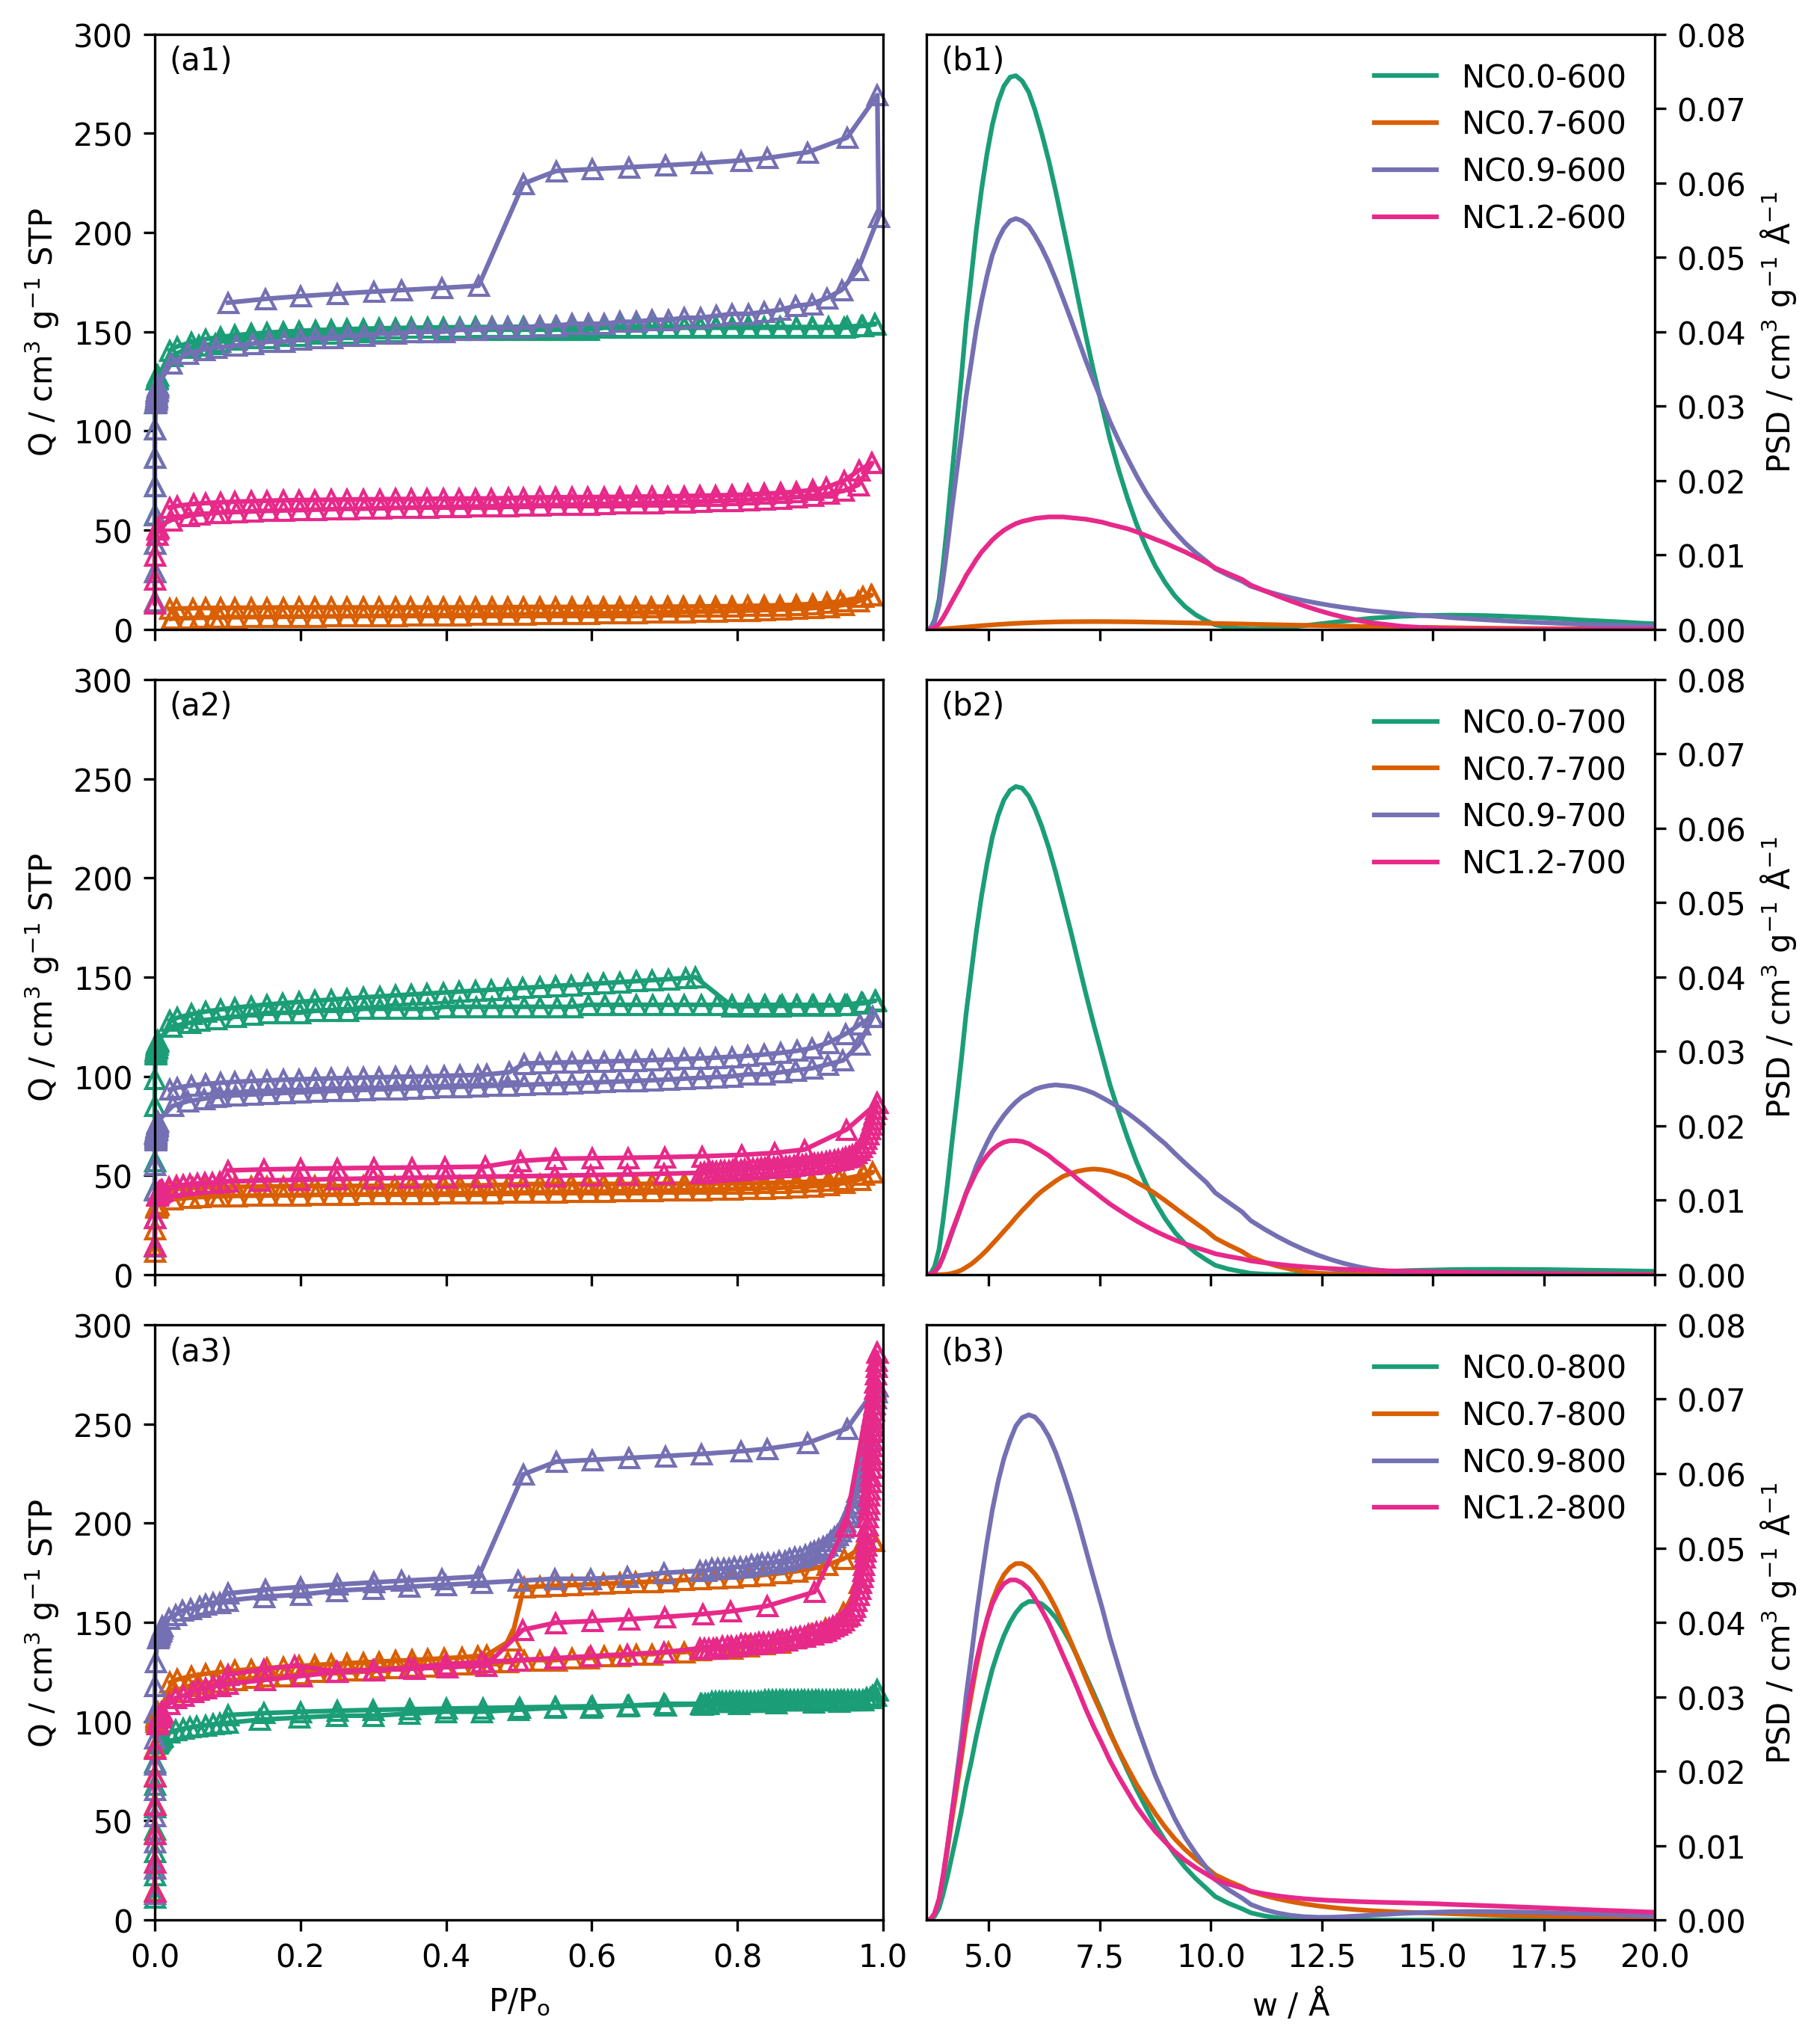
\includegraphics[width=\columnwidth, keepaspectratio]{4-impregnation/figs/NC_n2_isotherms.png}
    \caption{Isotherms (column a) and resultant PSDs (column b) for \acrshort{nc} samples activated at 600 (row 1), 700 (row 2), and 800 (row 3) \unit{\degreeCelsius}.}
    \label{fig:NC_n2_isotherms}
\end{figure}

Carbons derived from sodium carboxymethyl cellulose with a \acrshort{ds} between 0.7 and 1.2 consistently showed highest porosity at \acrshort{ds} of 0.9. While there is typically some optimum porogen:\ce{C} ratio for activation with \ce{NaOH} or \ce{KOH}, it is usually much higher than the extremely low value reported here.\citep{Sevilla2014Energy, Balahmar2017Biomass, tseng2006mesopore, Singh2019CO2, Boujibar2018CO2} A \acrshort{ds} of 0.9 corresponds to  an atomic \ce{Na}:\ce{C} ratio of just 0.12, while Balahmar \textit{et al.} reported that directly activated carbons from sawdust showed much higher $A_{BET}$ (\qty{1202}{\metre\squared\per\gram}) at a \ce{K}:\ce{C} atomic ratio of 0.19, which more than doubled when the amount of \gls{porogen} was doubled.\citep{Balahmar2017Biomass} Similarly, Tseng found that $A_{BET}$ of corn cob char-derived carbons was maximised at \qty{2500}{\metre\squared\per\gram} using a \ce{Na}:\ce{C} atomic ratio of 0.83. Indeed $V_t$ continued to increase as \ce{Na}:\ce{C} was increased to 1.3.\citep{tseng2006mesopore}\footnote{Atomic ratios not provided by original reports, determined by the author.} On the other hand, Roberts \textit{et al.} reported surface areas up to \qty{1051}{\metre\squared\per\gram}, for carbons derived from the pyrolysis of freeze-dried sodium poly(4-styrenesulfonate), which has an \ce{Na}:\ce{C} ratio of 0.13, similar to the sodium carboxymethyl cellulose reported here.\citep{Roberts2015Hierarchically} Indeed, others have corrobrated that polymeric salts with a similar amount of metal cation can produce carbons with similar surface areas.\citep{Yadav20123D, Puthusseri20143D, Hines2004Surface} These relatively high values for $A_{BET}$ at relatively low \gls{porogen}:\ce{C} ratios can be attributed to the development of porosity prior to oxidative chemical activation by the formation of cross-linkages between polymer chains. 


\paragraph{Hysteresis} Similarly to reported \ce{N2} isotherms on carbons derived from other polymeric salts,\citep{Roberts2015Hierarchically, Yadav20123D, Puthusseri20143D, Hines2004Surface} carbons produced in this work from sodium carboxymethyl cellulose show type I(a) character, with some degree of type II character and hysteresis (see figure \ref{fig:NC_n2_isotherms} (a1, a2, a3)). These hystereses appear to be permanent, as they are reproduced when the equilibration time is increased up to \qty{45}{\second} for the desorption branch, as shown in the appendix, figure \ref{fig:hyst}. According to the \acrshort{iupac} technical report on phyisorption and porosimetry, this hysteresis character is a result of network effects wherein wider pores only have access to the surface \textit{via} a much smaller pore entrance. During desorption this results in the larger pores remaining full until the narrow pore entrances are emptied at a much lower pressure.\citep{Thommes2015Physisorption} In their reports on polymeric salt-derived carbons, Hines \textit{et al.} and Yadav \textit{et al.} ascribe this behaviour to a mixed micro-/mesoporous structure.\citep{Yadav20123D, Hines2004Surface} The mesoporosity of the samples reported here is generally lower than those from polymeric sodium salts,\citep{Roberts2015Hierarchically, Yadav20123D} perhaps on account of the lower activation temperatures used in this work. Indeed, hysteresis is most prominent for samples activated at \qty{800}{\degreeCelsius}, and with the largest hyseresis occurring for samples derived from sodium carboxymethyl cellulose at a \acrshort{ds} of 0.9. This indicates that these network effects are dependent upon the harshness of the activation conditions. In particular, the reduction in the size of the hysteresis loop between samples NC0.9-800 and NC1.2-800 (figure \ref{fig:NC_n2_isotherms} (a3)) indicates that at a certain \ce{Na}:\ce{C} ratio, pore entrances are broadened by the action of the excess \gls{porogen}. The nature of the pore geometry and network connectivity may be investigated further by the use of a larger sorptive such as \ce{SF6}, as previously reported by Jagiello and others.\citep{LopezRamon1997Determination, Jagiello1995Adsorption, Navarro2006} The anomalously smaller hysteresis of all samples activated at \qty{700}{\degreeCelsius} requires further investigation, but may be connected to the high \ce{O} content of these samples as discussed in section \ref{sss:NC_composition}. 

\section{Conclusion}
\label{s:impregnation_conclusion}
This chapter has explored two alternative novel routes to the synthesis of \glspl{turbostratic carbon}, wherein it was attempted to increase \gls{porogen}-precursor contact, and improve the homogeneity of the distribution of the \gls{porogen}. In addition, the effect of small changes to the \gls{porogen}:precursor ratio was also studied, as well as \gls{activation} or \gls{htc} temperature. It was found that these techniques yield carbons which show unusual trends in porosity and elemental composition with respect to \glspl{turbostratic carbon} derived through more traditional techniques. 

In the case of carbons derived \textit{via} the hydrothermal impregnation of \ce{KOH} into sawdust, the extremely carbon-rich products were almost exclusively microporous. However, at a sufficiently high \ce{KOH}:\acrshort{sd} mass ratio (2.00), a carbon with extremely low density and unusually high mesoporosity (\qty{27}{\percent}) is produced. This is in contrast to sawudst-derived carbons derived through conventional activation methods. Such a product may be useful for electrochemical applications such as ion-transport.

On the other hand, the samples derived from the activation of sodium carboxymethyl cellulose give insight not only into the competitive pore-formation effects of polymeric cross-linking and oxidative chemical activation, but also show the fine control over porosity that is possible with the use of small, accurately quantified amounts of \gls{porogen}. The overall porosity of carbons in this set peaks at extremely low \gls{porogen}:\ce{C} atomic ratios (1.2), however what is more interesting is the indication of variations in pore network connectivity and/or pore geometry as shown by the synthetic condition-dependent appearance of hysteresis shown by \ce{N2} isothermal porosimetry. This apparent trend in porosity is mirrored by apparent changes in the composition of the carbons, indicating that it may be a function of the two competitive phenomena facilitating porogenesis from this precursor.

While the findings in this chapter give scope for a multitude of routes of further investigation, it is clear that as for the carbons in chapter \ref{ch:cbs}, \ce{N2} is insufficient as a probe molecule for accurately and thoroughly determining the porosity of these samples. In particular it appears that carbons in this work possess a high degree of ultramicroporosity, however the poor equilibration of the isotherms at low relative pressures means that precise \acrshortpl{psd} are impossible to determine. This has lead to the author exploring alternative techniques to attempt to understand the complex relationship between activation conditions and porosity in these unusual \glspl{turbostratic carbon} in chapter \ref{ch:dual_isotherm}.

\bibliographystyle{rsc}
\bibliography{bibliography/bib}
\chapter{Improved porosimetric techniques for highly ultramicroporous carbons}
\label{ch:dual_isotherm}

\newpage
\section*{Abstract}
It has been shown both in recent literature, and according to the work in chapters \ref{ch:cbs} and \ref{ch:impregnation} that porosimetry based on \ce{N2} isotherms at \qty{-196}{\degreeCelsius} is insufficient for the precise analysis of porosity in ultramicroporous carbons. This is a result of both \ce{N2}'s high quadrupole moment as well as its poor diffusion into \glspl{ultramicropore}. The investigation of alternative \glspl{adsorbate} for these materials, in particular \ce{H2} and \ce{O2} has shown some promise in this regard, and the development of the dual isotherm fitting method allows for a unified \acrshort{psd} to be determined with this method. As such this chapter investigates the relative utility of the simultaneous fitting of \ce{O2}/\ce{H2} isotherms to \acrfull{nldft} kernels in determining porosity of carbons found in this work, as compared to dual isotherm \ce{N2}/\ce{H2} as well as to single isotherm \acrshort{nldft} porosimetry and classical methods such as \acrshort{bet}. 

It was found that the \ce{O2}/\ce{H2} method provides an extremely high level of detail in the differences in porosity of carbons activated with differing amounts of \gls{porogen}. That is, not only can overall changes in porosity be observed, but more significantly very small changes in pore width are observable with this technique. The latter cannot be achieved using dual isotherm \ce{N2}/\ce{H2} fitting, or indeed by any other means investigated in this work. As a result, \ce{O2}/\ce{H2} analysis provides hints at pore formation mechanisms in these types of porous carbons that are not evident according to \ce{N2}/\ce{H2} analysis. Furthermore, it is apparent that the use of the \ce{H2} isotherm provides knowledge of porosity in the small \gls{ultramicropore} region which is inaccessible to either of the larger probes, \ce{O2} or \ce{N2}. Finally, the \acrshort{nldft} methodology used in this work provides quite different understanding of the variation of apparent surface area with synthetic conditions as compared to the traditional \acrshort{bet} method, which is likely a result of the greater suitability of the \acrshort{nldft} kernel to the analysis of ultramicroporous \glspl{turbostratic carbon} examined herein.
 
\newpage
\section{Experimental background}
\label{s:dual_intro}

\begin{figure}[b!]
    \centering
    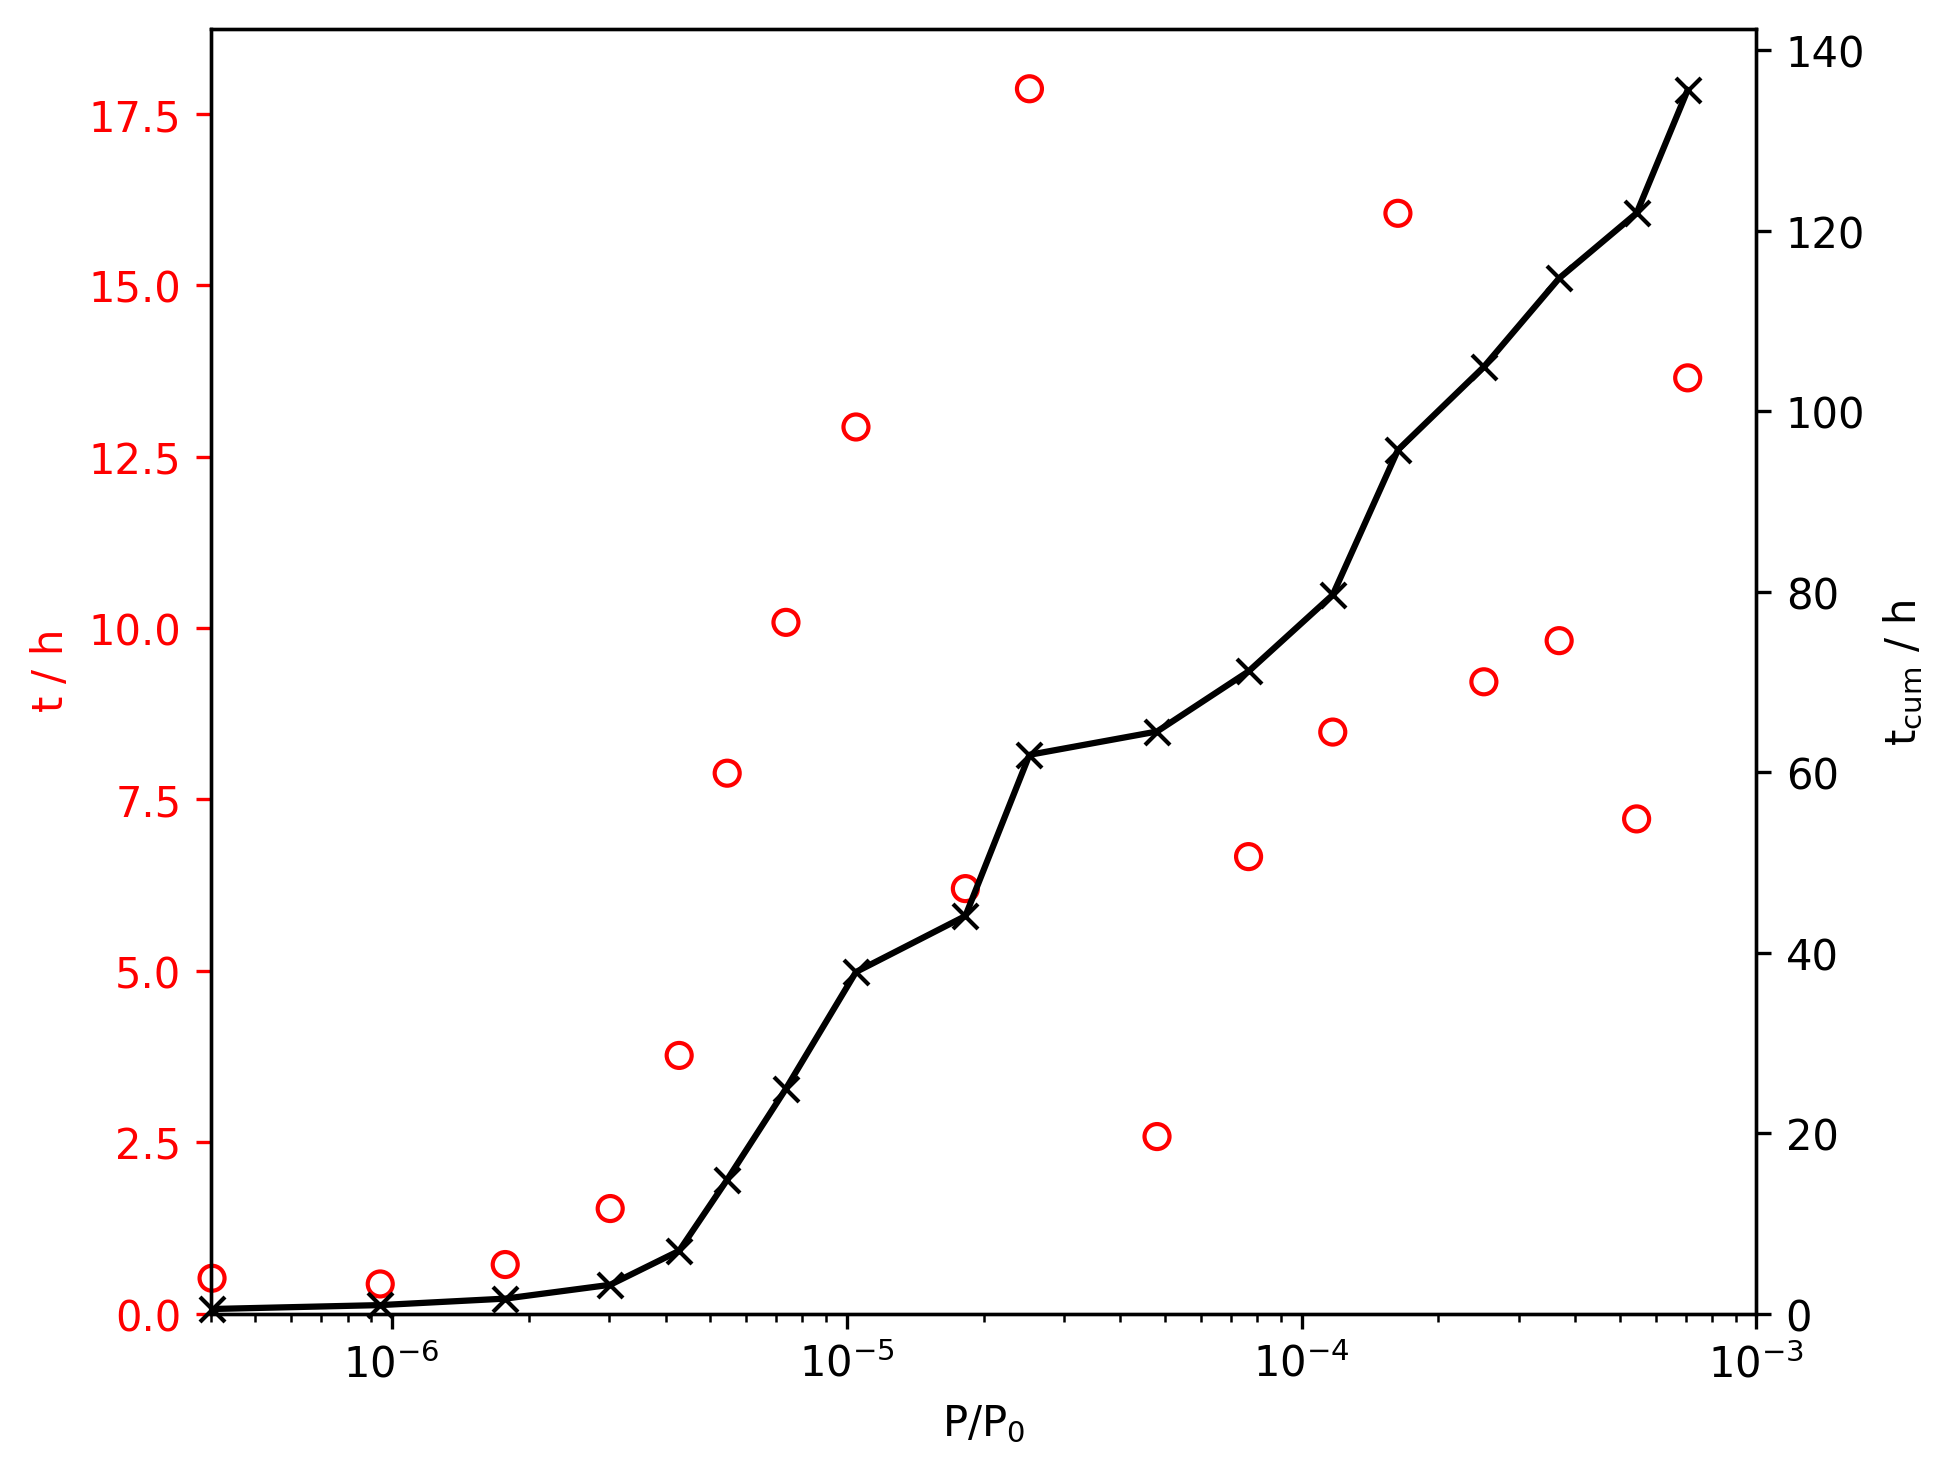
\includegraphics[width=0.95\columnwidth,keepaspectratio]{5-dual_isotherm/figs/timings.png}
    \caption{An example of the egregiously long equilibration times for individual points, $t$ and cumulative analysis time, $t_{cum}$ in the measurement of an \ce{N2} isotherm at \qty{-196}{\degreeCelsius} on sample hD-0700. The isotherm only reached a $P/P_0$ of $10^{-3}$ before being cancelled by the instrument.}
    \label{fig:timings}
\end{figure}

In chapters \ref{ch:cbs} and \ref{ch:impregnation}, it became clear that derivation of \acrshortpl{psd} and related porosimetric values from the typical \ce{N2} (\qty{-196}{\degreeCelsius}) isotherm was not sufficiently accurate. In particular, for carbons with a low degree of activation isotherm measurement became impractical due to extremely long equilibration times - see figure \ref{fig:timings}. In many cases this resulted in limited isotherms that do not include points at ultra-low pressures ($P/P_0 < 10^{-4}$) (examples of such isotherms are shown in figures \ref{fig:0TTT_psdisofull}, \ref{fig:NCxx-600_psdisofull}-\ref{fig:NCxx-800_psdisofull}). \acrshort{psd}s from these incomplete and/or poorly equilibrated isotherms indicate a high degree of porosity in the \gls{ultramicropore} region, however \glspl{ultramicropore} fill at ultra-low pressures. Thus, as noted in previous chapters there can be very minimal confidence in the results derived from this technique. This issue has been reported as early as 1982.\citep{RodriguezReinoso1982Activated} A solution in the literature to this problem has been to employ \ce{CO2} isotherms at \qty{0}{\degreeCelsius} in order to probe \glspl{ultramicropore} and small \glspl{supermicropore}.\citep{Jagiello2004Comparison, Jagiello2015Dual, Garrido1987Use, LozanoCastello2004Usefulness} The porosity up to some upper-limit (usually taken as somewhere around \qty{10}{\angstrom}) can then be calculated.\citep{furimsky2000characterization, sing1989use} \acrshort{psd}s have also been calculated from these isotherms,\citep{Jagiello2004Comparison} and indeed Jagiello and co-workers have developed techniques to fit \acrshort{nldft} kernels simultaneously to \ce{CO2} and \ce{N2} isotherms.\citep{Jagiello2019Enhanced, Jagiello2015Dual} However, in the case of \glspl{turbostratic carbon}, the effect of the quadrupole moment of both \ce{CO2} and \ce{N2} on the accuracy of the resultant \acrshort{psd} means that the much less polar \ce{H2} and \ce{O2} are now becoming common replacements to elucidate the full porosity of such materials.\citep{Jagiello2020Exploiting, Blankenship2022Confirmation, GrauMarin2020Evaluation} Furthermore, \ce{O2} and \ce{H2} isotherms can be measured at \qty{-196}{\degreeCelsius}, unlike \ce{CO2} which is solid at this temperature - thus eliminating the need to change temperature control apparatus. Therefore, this chapter investigates the relative utility of both \ce{N2}/\ce{H2} and \ce{O2}/\ce{H2} pairs in determining \acrshortpl{psd} of the ultramicroporous carbons produced in chapters \ref{ch:cbs} and \ref{ch:impregnation}.

\section[Exploring alternative porosimetric adsorbates]{Exploring alternative porosimetric \glspl{adsorbate}}
\label{s:dual_initial}
Section \ref{s:dual_intro} laid out the need to explore alternative porosimetric techniques for analysis of the ultramicroporous carbons produced in previous chapters. While a comprehensive comparison of dual fitting to \ce{N2}/\ce{H2} and \ce{O2}/\ce{H2} isotherm pairs is detailed in \ref{pub:dual_iso} (contained in this chapter), what follows here are the results of some initial analytical experiments using \ce{N2} and \ce{O2}, and combined \ce{O2}/\ce{H2} isotherms.

While the purpose of this chapter is to use more advanced, \acrshort{nldft} techniques in the determination of porosity from \gls{physisorption} isotherms, comparing the classical measures of surface area and pore volume yielded by \ce{N2} and \ce{O2} isotherms at \qty{-196}{\degreeCelsius} also gives some interesting insights. Results of these analyses are displayed in table \ref{tb:n2_o2_classical}. The important distinctions between these \glspl{adsorbate} are their molecular cross-sectional areas ($\sigma$), kinetic diameters ($d_k$) and quadrupole moments ($\mu$). As stated before, \ce{O2} is significantly less polar than \ce{N2}, these \glspl{adsorbate} having $\mu$ of 0.155 and 0.697 respectively.\citep{Lide2007Handbook, Poling2001Properties, Graham1998Measurement} In terms of $d_k$ they are similar, and $\sigma_{O_2}$ is only slightly smaller than $\sigma_{N_2}$ at \qtylist[list-units=single]{0.143; 0.162}{\nm\squared}  respectively. However, it should be noted that there is no definitive, exact value for these $\sigma$ values as they vary according to the surface the molecule is being adsorbed onto.\citep{kodera1959molecular, kodera1960molecular, livingston1949cross} This variability is much more significant in the case of \ce{N2} due to its greater polarity - indeed $\sigma_{N_2}$ can vary for individual molecules of \ce{N2} on a single \gls{adsorbent} at different \gls{adsorption} sites.\citep{Jagiello2020Exploiting}

\begin{table}[b!]
    \centering
    \caption{Comparison of classical measures of porosity derived using \ce{N2} and \ce{O2} porosimetry. $A_{BET}$ calculated using the Rouquerol method,\citep{Rouquerol2007Is} and $V_t$ using the single-point approach. Values in brackets indicate the microporous portion of surface area and pore volume as determined by t-plot using a Carbon Black STSA thickness curve. The two hD-0700 samples in table are repeat syntheses of the same sample. }
    \begin{tabularx}{\textwidth}{lXlXlXlXl}
    \toprule
        \textbf{Sample} & \multicolumn{4}{c}{$\mathbf{A_{BET}}$ \textbf{/ \unit[detect-weight]{\metre\squared\per\gram}}} &  \multicolumn{4}{c}{$\mathbf{V_t}$ \textbf{/ \unit[detect-weight]{\cm\cubed\per\gram}}} \\
        & \multicolumn{2}{c}{\textbf{\ce{N2}}} & \multicolumn{2}{c}{\textbf{\ce{O2}}} & \multicolumn{2}{c}{\textbf{\ce{N2}}} & \multicolumn{2}{c}{\textbf{\ce{O2}}} \\
    \midrule
        NC0.0-800 & 449 & (408) & 595 & (532) & 0.17 & (0.13) & 0.24 & (0.20) \\
        NC0.7-800 & 580 & (495) & 645 & (563) & 0.21 & (0.16) & 0.25 & (0.18) \\
        NC0.9-800 & 669 & (578) & 876 & (749) & 0.28 & (0.22) & 0.37 & (0.29) \\
        \\
        SA1.00-200 & 1410 & (1306) & 1513 & (1333) & 0.61 & (0.54) & 0.62 & (0.51)  \\
        \\
        SA0.00-250 & 949 & (838) & 596 & (514) & 0.18 & (0.16) & 0.25 & (0.20) \\
        SA0.50-250 & 906 & (826) & 1161 & (1066) & 0.51 & (0.47) & 0.40 & (0.34) \\
        SA1.00-250 & 1081 & (971) & 1266 & (1138) & 0.54 & (0.48) & 0.45 & (0.37) \\
        \\
        hD-0700\textit{(1)} & 278 & (242) & 428 & (355) & 0.18 & (0.11) & 0.16 & (0.12) \\
        hD-0700\textit{(2)} & 317 & (265) & 411 & (346) & 0.19 & (0.12) & 0.15 & (0.11) \\
    \bottomrule
    \end{tabularx}
    \label{tb:n2_o2_classical}
\end{table}

These issues with these classical analyses notwithstanding, the values for $A_{BET}$ derived from \ce{O2} porosimetry are generally higher than that from \ce{N2}. The relative percentage of surface area taken up by \glspl{micropore} is however consistent from both techniques, being between \qtylist[list-units=single]{83;92}{\percent} for all samples. On the other hand, $V_t$ does not show any consistency in the way it varies between the two techniques. It is likely that simply due to the large uncertainties in determination of pore volume \textit{via} the single-point method, any pattern is obscured. The increases in $A_{BET}$ found when using \ce{O2} at \qty{-196}{\degreeCelsius} as a molecular probe may indicate the ability of \ce{O2} to diffuse into pores inaccessible to \ce{N2}. It is also interesting to note that $A_{BET}$ is far more consistent for the two repeats of hD-0700 when determined using \ce{O2} rather than \ce{N2}, perhaps giving further indication of the improvements in reliability of results attained using this alternative \gls{adsorbate}. It is however difficult to categorically assert \ce{O2}'s superiority over \ce{N2} for this application from this evidence, due to the aforementioned problems with these classical techniques. 

\begin{figure}[hptb]
    \centering
    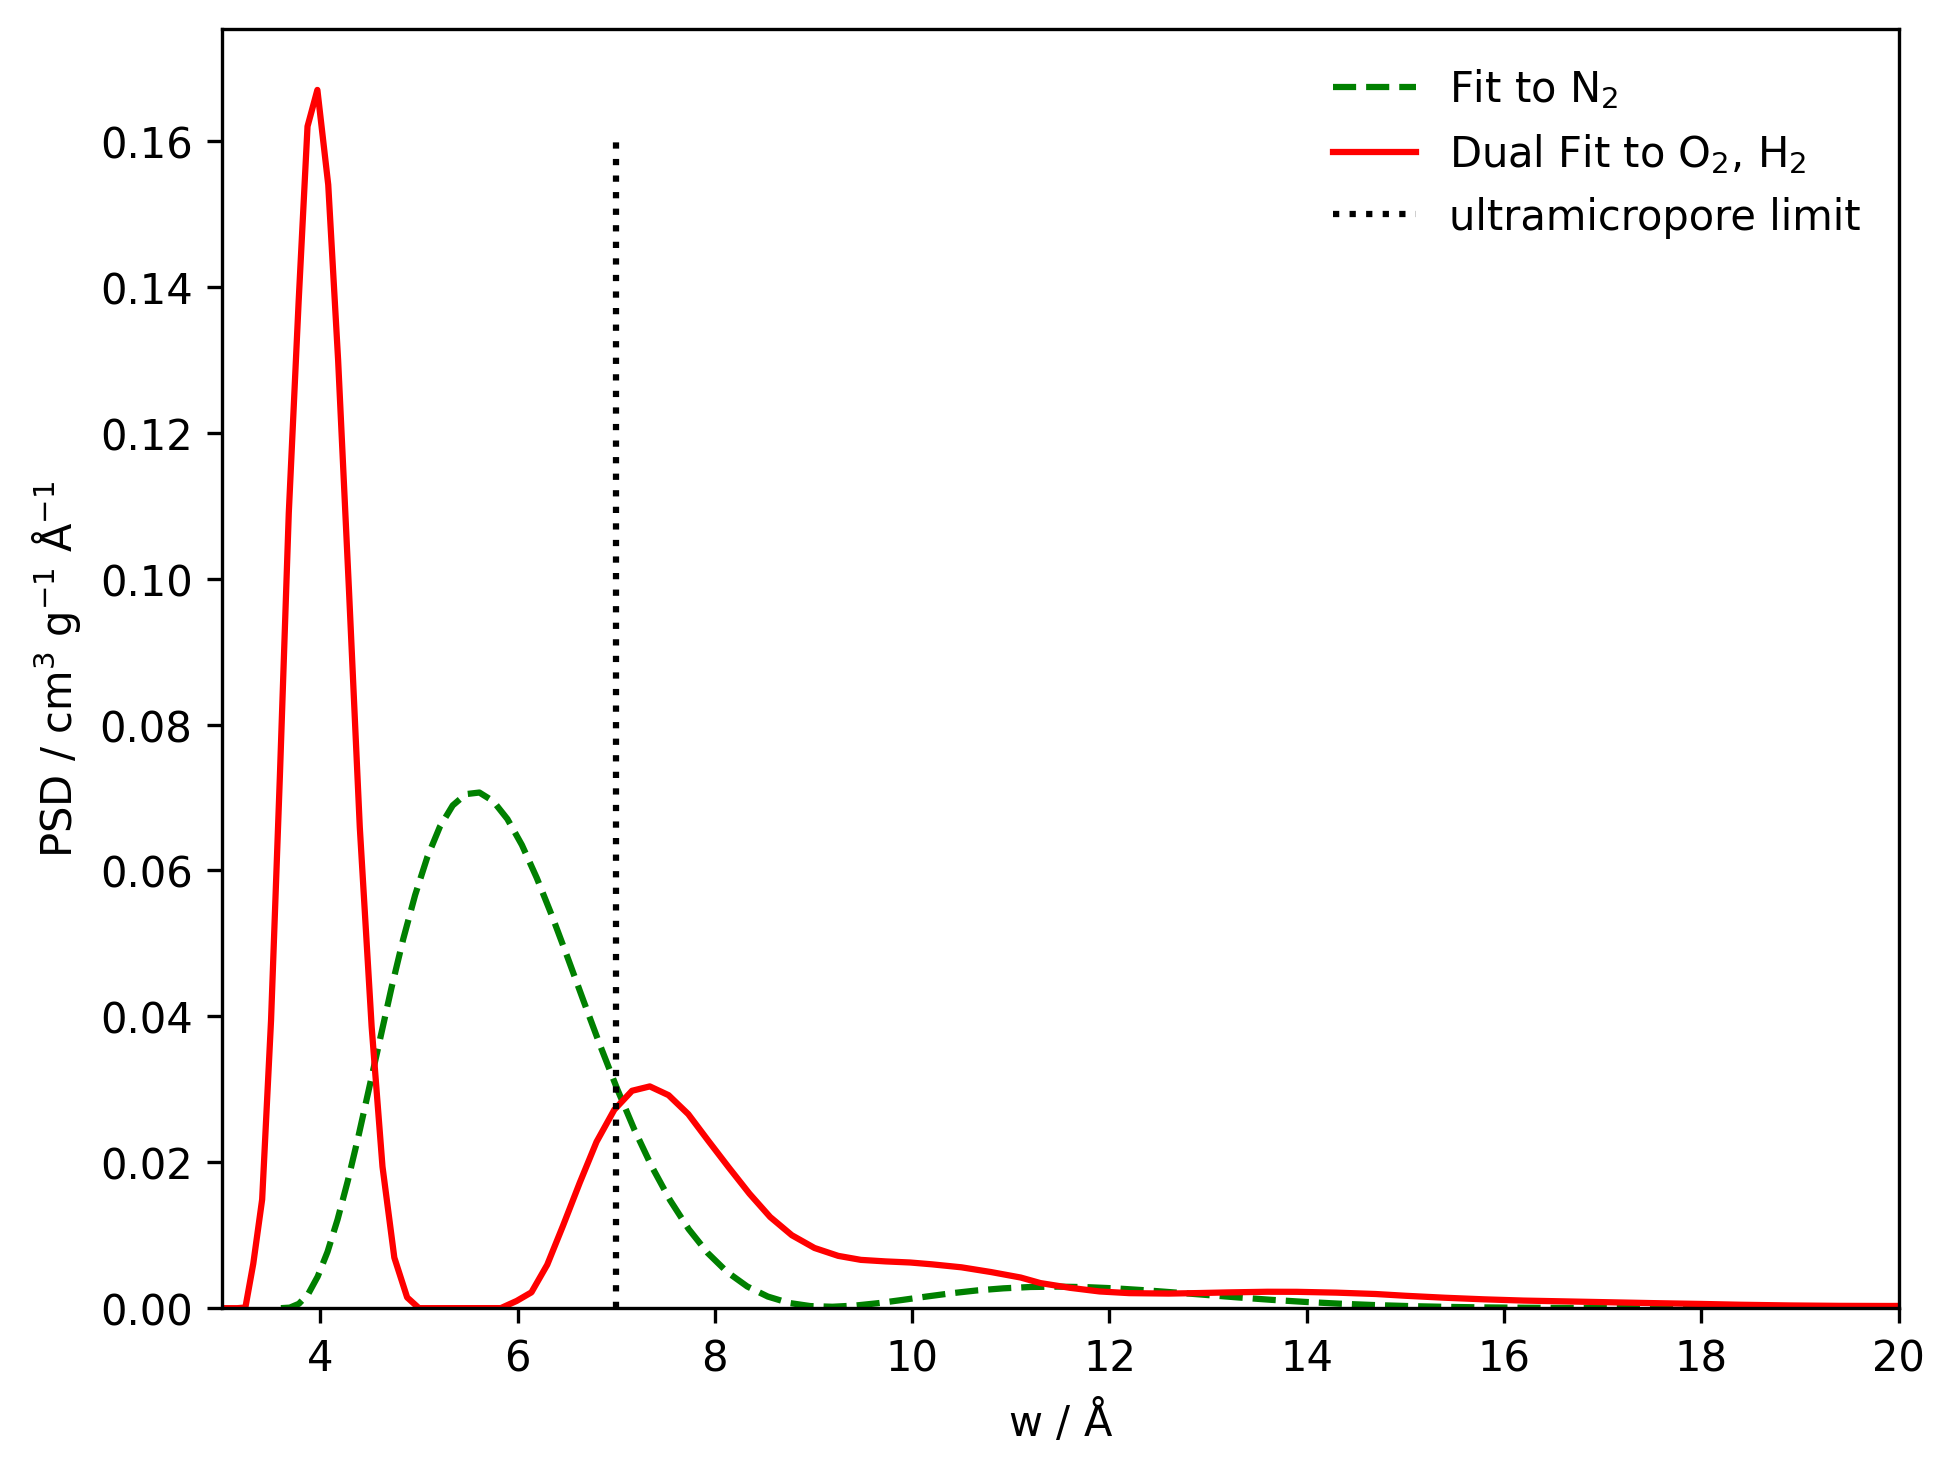
\includegraphics[width=\columnwidth, keepaspectratio]{5-dual_isotherm/figs/dual_psd_compare.png}
    \captionof{figure}{An example of the different \acrshortpl{psd} from single fit to \ce{N2} and dual fit to \ce{O2} and \ce{H2} isotherms on sample SA0.00-250. The \gls{ultramicropore} limit is also shown; clearly the dual fit shows a separation in pore regions that is different to the \gls{ultramicropore} limit of \qty{7.0}{\angstrom}. \newline}
    \label{fig:dual_psd_compare}
    
    \captionof{table}{Pore volume ($V_{NLDFT}$) and surface area ($A_{NLDFT}$) of selected samples from chapters \ref{ch:cbs} and \ref{ch:impregnation} in the \gls{micropore} region, divided into two regions according to the local minimum ($w_{locmin}$). Porosities calculated with simultaneous fit of 2D-NLDFT-HS kernels to \ce{O2} and \ce{H2} isotherms.}
    \begin{tabularx}{\textwidth}{llXXXX}
    \toprule
        \textbf{Sample} & $\mathbf{w_{locmin}}$ \textbf{/ \unit[detect-weight]{\angstrom}} & \multicolumn{2}{c}{$\mathbf{V_{NLDFT}}$ \textbf{/ \unit[detect-weight]{\cm\cubed\per\gram}}} & \multicolumn{2}{c}{$\mathbf{A_{NLDFT}}$ \textbf{/ \unit[detect-weight]{\metre\squared\per\gram}}} \\
        & & \textbf{1} & \textbf{2} & \textbf{1} & \textbf{2} \\
    \midrule
        NC0.0-800 & 5.5 & 0.14 & 0.09 & 715 & 184 \\
        NC0.7-800 & 5.3 & 0.12 & 0.15 & 620 & 366 \\
        NC0.9-800 & 5.4 & 0.13 & 0.20 & 669 & 507 \\
        \\
        SA1.00-200 & 6.1 & 0.20 & 0.38 & 868 & 824 \\
        \\
        SA0.00-250 & 5.4 & 0.12 & 0.33 & 627 & 811 \\
        SA0.50-250 & 6.1 & 0.17 & 0.35 & 812 & 820 \\
        SA1.00-250 & 6.1 & 0.19 & 0.37 & 841 & 195 \\
        \\
        hD-0700\textit{(1)} & 5.7 & 0.10 & 0.10 & 464 & 217 \\
        hD-0700\textit{(2)} & 5.5 & 0.09 & 0.09 & 444 & 217 \\
    \bottomrule
    \end{tabularx}
    \label{tb:finepore}
\end{figure}

Initial investigations into dual isotherm analysis were for the purpose of comparing porosity as given by fitting of the 2D-NLDFT-HS kernel to \ce{N2} isotherms to that determined by the dual fitting of the appropriate 2D-NLDFT-HS kernels to \ce{O2} and \ce{H2} isotherms on carbon samples that appear to have a high proportion of \glspl{ultramicropore}. An example of this comparison is shown in figure \ref{fig:dual_psd_compare}. In general, it was found that the dual \ce{O2}/\ce{H2} fit yields greater overall porosity than the single isotherm fit. Furthermore, the \acrshort{psd}s are consistently bimodal for the dual isotherm fit. While \glspl{micropore} are typically subdivided at \qty{7.0}{\angstrom} into \glspl{ultramicropore} and \glspl{supermicropore} (as indicated by the dotted line in figure \ref{fig:dual_psd_compare}), the minimum between the two regions is at a consistently lower pore width than this. For this purpose, the pore volume ($V_{NLDFT}$) and surface area ($A_{NLDFT}$) are given in table \ref{tb:finepore} as subdivided into these two regions according to the variable local minimum ($w_{locmin}$). The separate regions appear to be a result of different probeable pore sizes of the two adsorptives; an issue which is discussed in more depth in \ref{pub:dual_iso}, \textbf{section 3.3.1.}. 


The proportion of \glspl{micropore} taken up by these lower width peaks (peak 1) varies, with $V_{NLDFT}$ ranging from \qtyrange[list-units=single]{27}{61}{\percent} and $A_{NLDFT}$ from \qtyrange[list-units=single]{44}{81}{\percent} (see table \ref{tb:finepore}). This variation appears to be inversely related to degree of activation and indeed is the topic of \ref{pub:dual_iso}. In the case of the NC\textit{x.x-TTT} and SA\textit{x.xx}-250 samples it is clear that the proportion of microporosity taken up by the initial peak falls precipitously with \gls{porogen}:precursor ratio. The consistency found between the two repeats of hD-0700 (see table \ref{tb:n2_o2_classical}) when using \ce{O2} to determine classical measures of porosity is also present with these dual isotherm 2D-NLDFT-HS analyses. This lends further credence to the notion that the dual isotherm porosimetric method explored here may be superior to current, single isotherm methods.

The finer detail attained in the derived \acrshortpl{psd} from the dual \ce{O2}/\ce{H2} fits is of great interest as \glspl{ultramicropore} have been attributed to the low pressure uptake of \glspl{adsorbate} such as \ce{CO2} and \ce{H2}.\citep{Presser2011Effect, Sevilla2014Energy, Cabria2007optimum, DelaCasaLillo2002Hydrogen, Masika2012Hydrogen} What has not yet been investigated is the comparison of dual \ce{N2}/\ce{H2} fits with \ce{O2}/\ce{H2}. This, therefore is investigated in \ref{pub:dual_iso}. Furthermore, the work in chapter \ref{ch:pyPUC} shows that the porosity as shown by these dual isotherm techniques does have physical significance at least in terms of \ce{CO2} uptake capacity.
%
\newpage
\section[Publication I]{Publication I: Confirmation of pore formation mechanisms in biochars and activated carbons by dual isotherm analysis}

\textbf{Contribution of the author}: The author performed all synthesis and instrumental analysis of samples in the work, analysed the results and wrote the manuscript.

\textbf{Note}: For this publication, the sample names are slightly different. The variable \textit{x.xx} in SA\textit{x.xx-HHH} samples is truncated to \textit{x.x}, i.e. SA0.5-250 in the publication is equivalent to SA0.50-250 in chapter \ref{ch:impregnation}. As for NC\textit{x.x-TTT} samples only samples with \textit{TTT} of \qty{800}{\degreeCelsius} are examined, thus NC0.9 is identical to NC0.9-800 in chapter \ref{ch:impregnation}.  

\setcounter{opagenum}{\thepage}
\newpage

\setlength{\originalVOffset}{\voffset}   
\setlength{\originalHOffset}{\hoffset}

\setlength{\voffset}{0cm}
\setlength{\hoffset}{0cm}
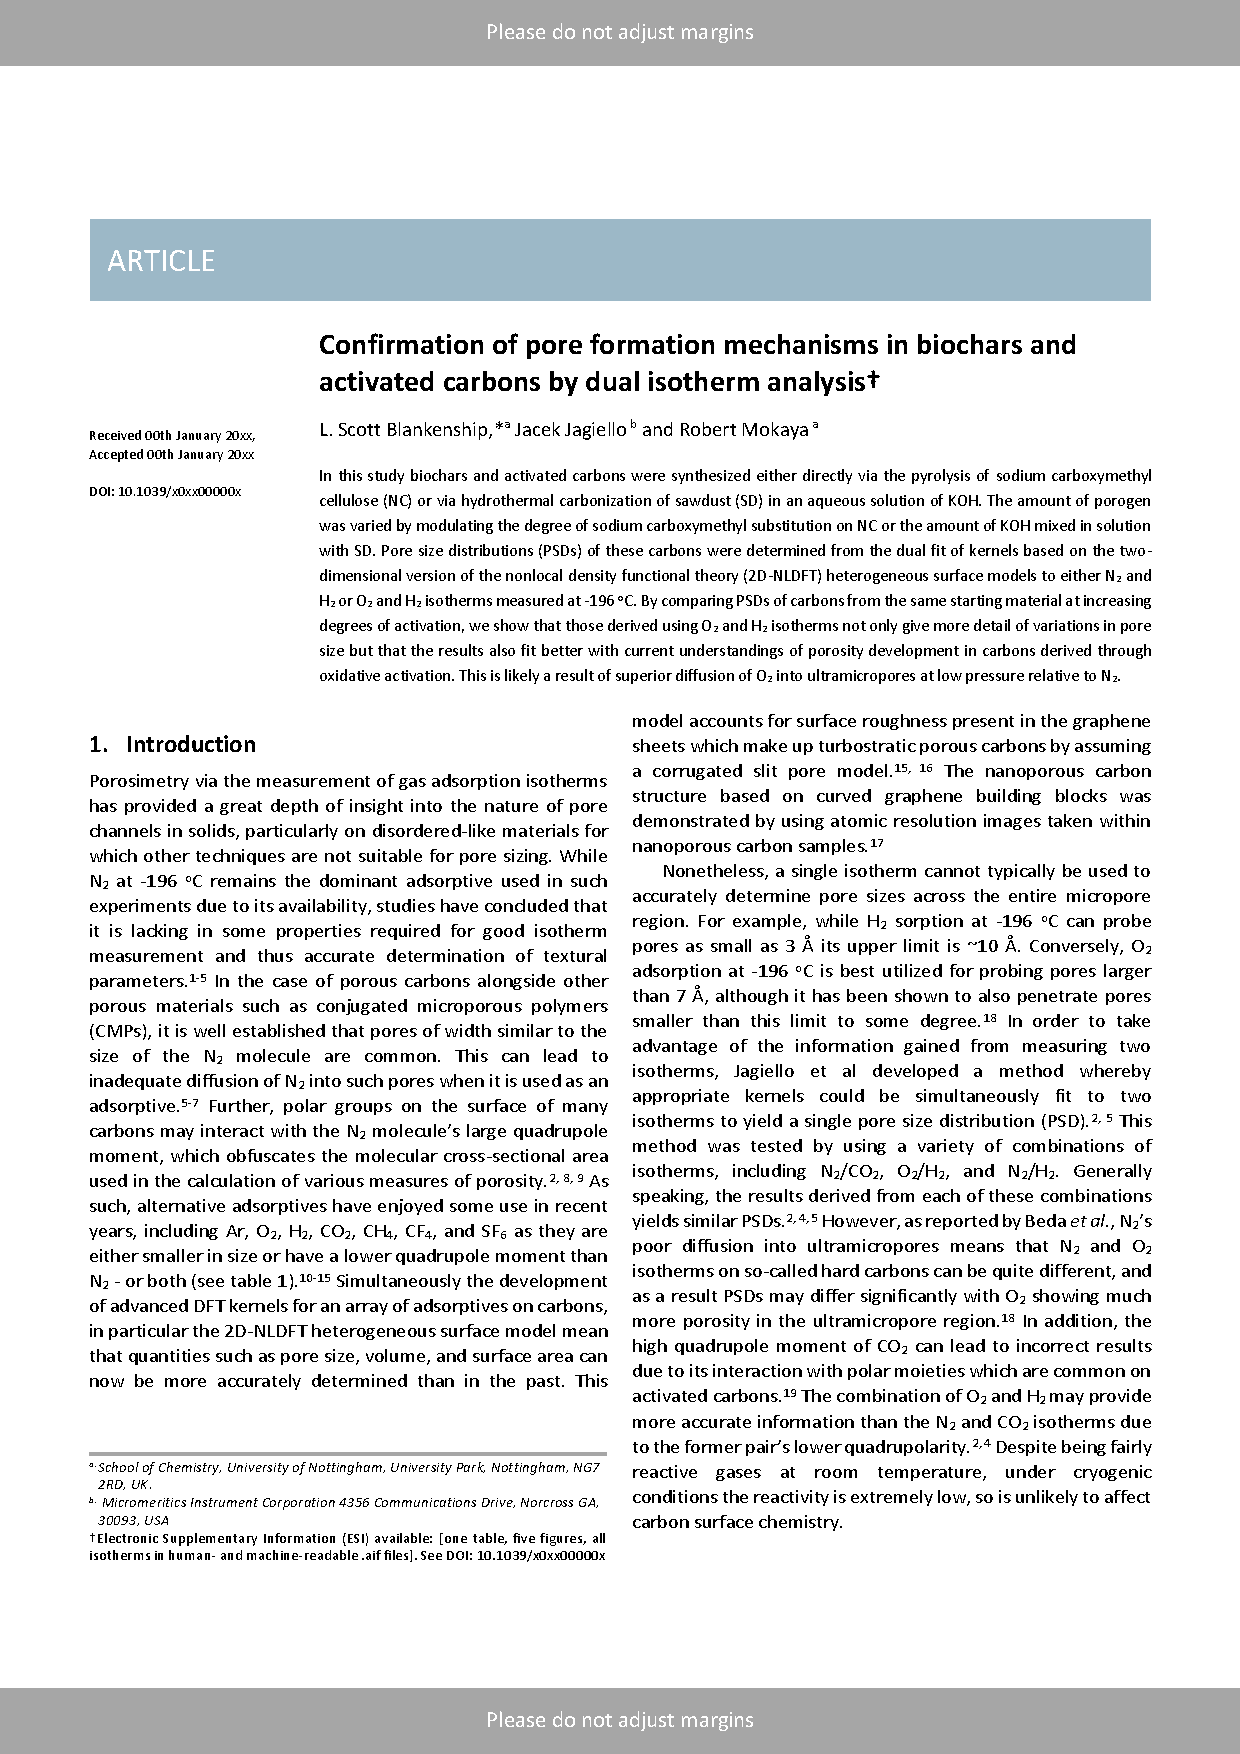
\includepdf[pagecommand={
    \setcounter{page}{\theopagenum}
    \thispagestyle{empty}
    },
    pages=-]{5-dual_isotherm/publication_02.pdf}
\setlength{\voffset}{\originalVOffset}
\setlength{\hoffset}{\originalHOffset}

\newpage
\section{Further analysis}
\ref{pub:dual_iso} contains only the \acrshortpl{psd} from the analysis of the SA\textit{x.xx}-250 and SA\textit{x.xx}-300 series as well as NC\textit{x.x}-800 series for \textit{x.x} in the range 0.0 to 0.9. Since publication, dual isotherm analyses of SA0.50-200, SA1.00-200 and NC1.2-800 has been completed. A discussion of the results follows here, particularly in relation to the utility of dual isotherm analyses on monitoring \acrshort{psd} development with changes in sample preparation conditions.

As discussed in section \ref{ss:sd_results}, the classically derived porosities of samples synthesised from \acrfull{sd} with identical \ce{KOH}:\acrshort{sd} ratios, do not vary significantly with \acrshort{htc} temperature. Nonetheless, it is interesting to compare such results using different porosimetric techniques. The \acrshortpl{psd} and associated fits are displayed in the appendix, figures \ref{fig:SA050-xxx_isopsd}, \ref{fig:SA100-xxx_isoposd}. While the dual \ce{O2}/\ce{H2} fits do appear to show small shifts in the position of the second maximum in the \acrshort{psd} for SA0.50-\textit{HHH} samples with hydrothermal impregnation temperature (see figure \ref{fig:SA050-xxx_isopsd}(2P)), this is not evident for SA1.00-\textit{HHH} samples (figure \ref{fig:SA100-xxx_isoposd}(2P)). Indeed it could be concluded that the dual \ce{N2}/\ce{H2} fits show just as much variation in the position of the second maximum. Thus, the \acrshort{psd} broadening observed in \ref{pub:dual_iso} according to dual isotherm \ce{O2}/\ce{H2} analysis is apparently only associated with \ce{KOH}:\acrshort{sd} ratio, as opposed to hydrothermal impregnation temperature.

\begin{figure}[hptb]
    \centering
    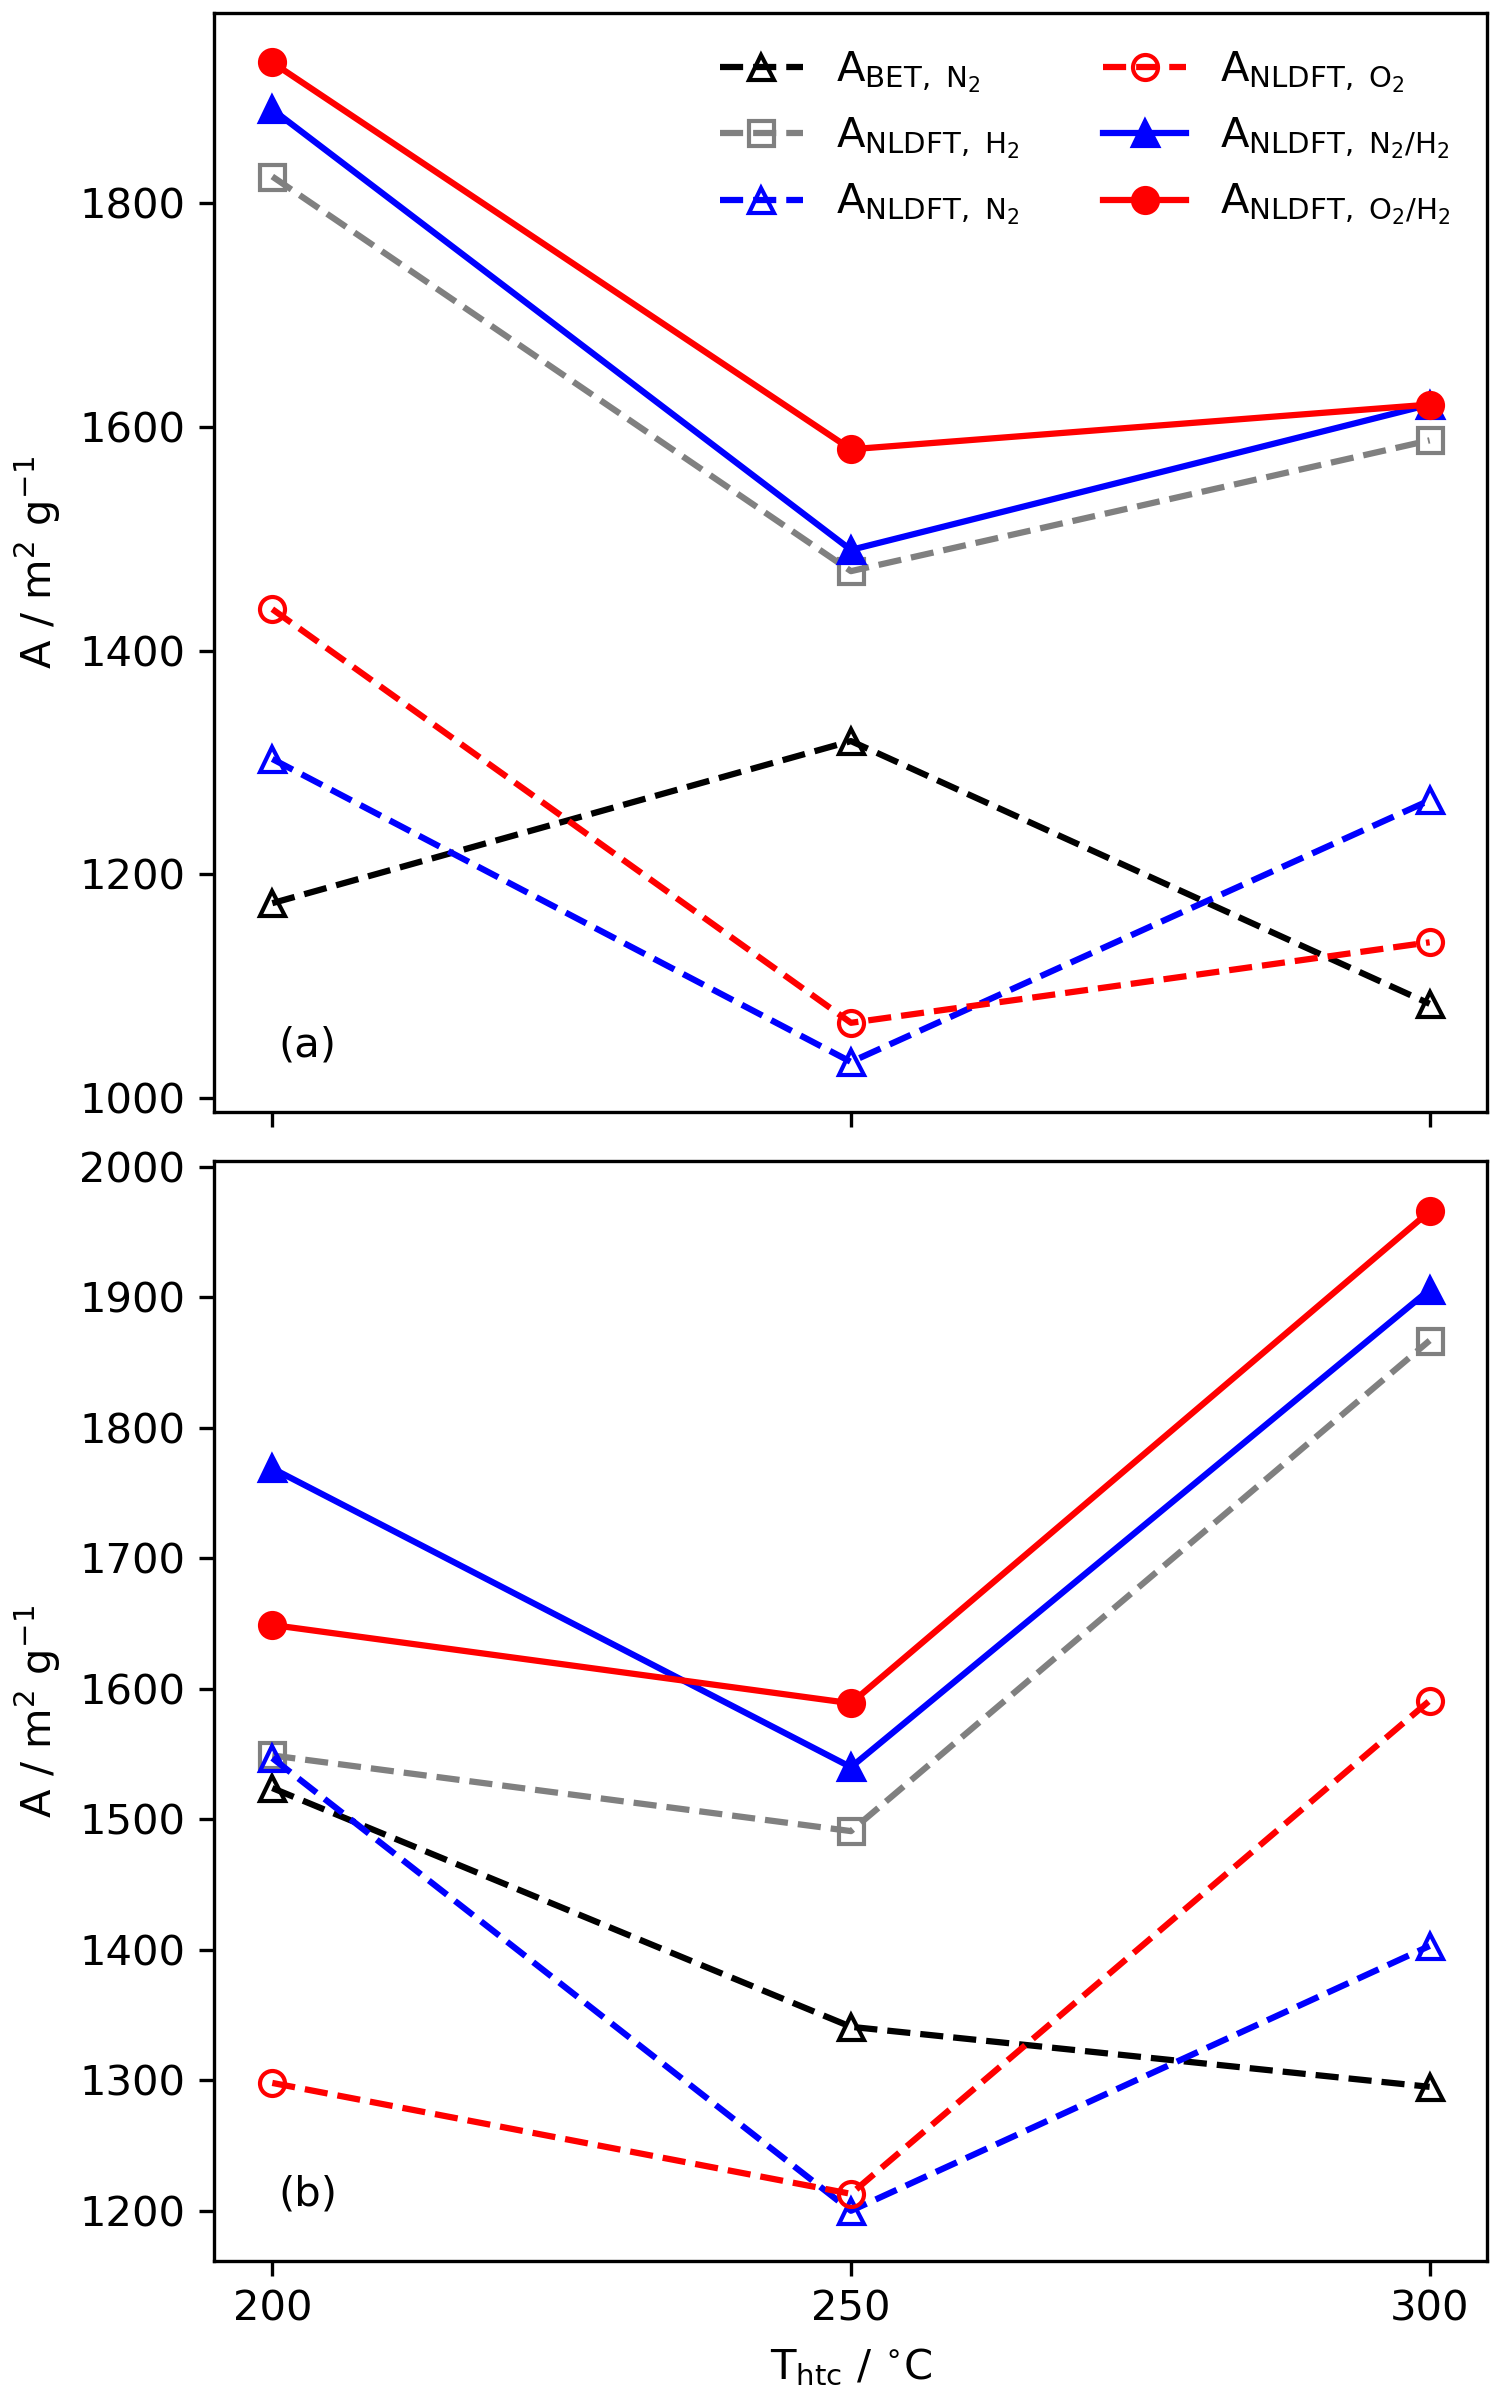
\includegraphics[width=0.95\columnwidth,keepaspectratio]{5-dual_isotherm/figs/SD_classical_nldft.png}
    \caption{Trends in surface area with hydrothermal impregnation temperature $T_{htc}$ of \acrshort{sd}-derived carbons, as determined \textit{via} the BET method as well as from fitting of 2D-NLDFT-HS kernel to \ce{H2}, \ce{N2}, \ce{O2} isotherms as well as dual-fitting to \ce{N2}/\ce{H2} and \ce{O2}/\ce{H2} pairs. Subfigures (a) and (b) are for \ce{KOH}:\acrshort{sd} ratios of 0.50 and 1.00 respectively.}
    \label{fig:classical_nldft_compare}
\end{figure}

A comparison of the trends in apparent surface area with hydrothermal carbonisation temperature ($\rm T_{htc}$) as determined by the \acrshort{bet} method on an \ce{N2} isotherm,\citep{Brunauer1938Adsorption} as well as \textit{via} fitting of 2D-NLDFT-HS kernels to \ce{N2}, \ce{O2}, \ce{H2} isotherms and dual fitting to \ce{N2}/\ce{H2}, \ce{O2}/\ce{H2} pairs is shown in figure \ref{fig:classical_nldft_compare}. For samples derived with both \ce{KOH}:\acrshort{sd} ratios of 0.50 and 1.00, the 2D-NLDFT method consistently shows a minimum in apparent surface area at $T_{htc}$ of \qty{250}{\degreeCelsius}. This is in contrast to $A_{BET,N_2}$ which shows a \textit{maximum} at this temperature for \ce{KOH}:\acrshort{sd} of 0.50, and a consistent decrease with temperature when the ratio is 1.00. Thus this discrepancy in the trend is likely a result of the inadequacy of the BET method for determining surface area in microporous materials, rather than an artefact of the nature of \ce{N2} \gls{adsorption}. Namely, the BET method relies on the formation of a monolayer in order to accurately quantify surface area, which is not possible in \glspl{micropore} as the probe molecule kinetic diameter is of the same order as the distance between pore walls (i.e. the pore width, $w$).\citep{Rouquerol2007Is, coasne2004grand, ambroz2018evaluation, walton2007applicability} Furthermore, the nature of the \gls{adsorption} is uncertain, as it is unknown to what degree the probe molecule is adsorbed on each of the pore walls in the (apparently) slit-shaped pores.\citep{Rouquerol2007Is, Brunauer1938Adsorption} \acrshort{nldft}-derived porosity, and in particular surface area determination does not have these assumptions that are unsuitable for highly microporous materials. Indeed, the kernel of model isotherms used in the 2D-NLDFT-HS method\citep{Jagiello20132D} is specifically designed for and suited to this kind of material. 

Of further interest are the relative apparent surface areas determined by each probe molecule using the 2D-NLDFT-HS method. \ce{O2} and \ce{N2} single fits give approximately similar values and are in a similar range as those derived using $A_{BET}$. Simultaneously dual isotherm \ce{O2}/\ce{H2} and \ce{N2}/\ce{H2}, as well as single isotherm \ce{H2} derived areas match well with one another, but give significantly higher values than the previously mentioned methods. This further confirms that the use of \ce{H2} as a probe molecule allows for the penetration of pores inaccessible to the larger \ce{O2} and \ce{H2} as was mentioned in \ref{pub:dual_iso}. The similarity in apparent surface areas derived using \ce{H2} alone, with the dual fit methods for a \ce{KOH}:\acrshort{sd} ratio of 0.50 is striking, indicating that all relevant porosity is accessible by \ce{H2} for these materials. There is greater discrepancy when \ce{KOH}:\acrshort{sd} is increased to 1.00, probably a result of \acrshort{psd} broadening through more aggressive action of the \gls{porogen}, and thus creating porosity accessible to \ce{N2} or \ce{O2} but which will not be filled by \ce{H2} at pressures up to \qty{1}{\bar}.

In section \ref{ss:NC}, a surprising reduction in total porosity for \textit{x.x} of 1.2 was discussed. That is, while increasing the \acrfull{ds} of \ce{Na} from 0.7, to 0.9 porosity increases ($A_{BET}$ and $V_t$), but these metrics reduce again when \acrshort{ds} is increased further to 1.2 (see table \ref{tb:nc_porosity}). This drop in overall porosity is also accompanied by small reductions in \% microporosity, and the trend occurs regardless of activation temperature. The more advanced techniques detailed in this chapter should give more detail as to the changes in porosity, and as such the \acrshortpl{psd} and associated isotherms and fits are shown in figure \ref{fig:NC_contraction}. This is of course a reproduction of \textbf{figure 3} in \ref{pub:dual_iso}, but with the inclusion of NC1.2-800 (referred to as NC1.2 in the publication).  

\begin{figure}[ht!]
    \centering
    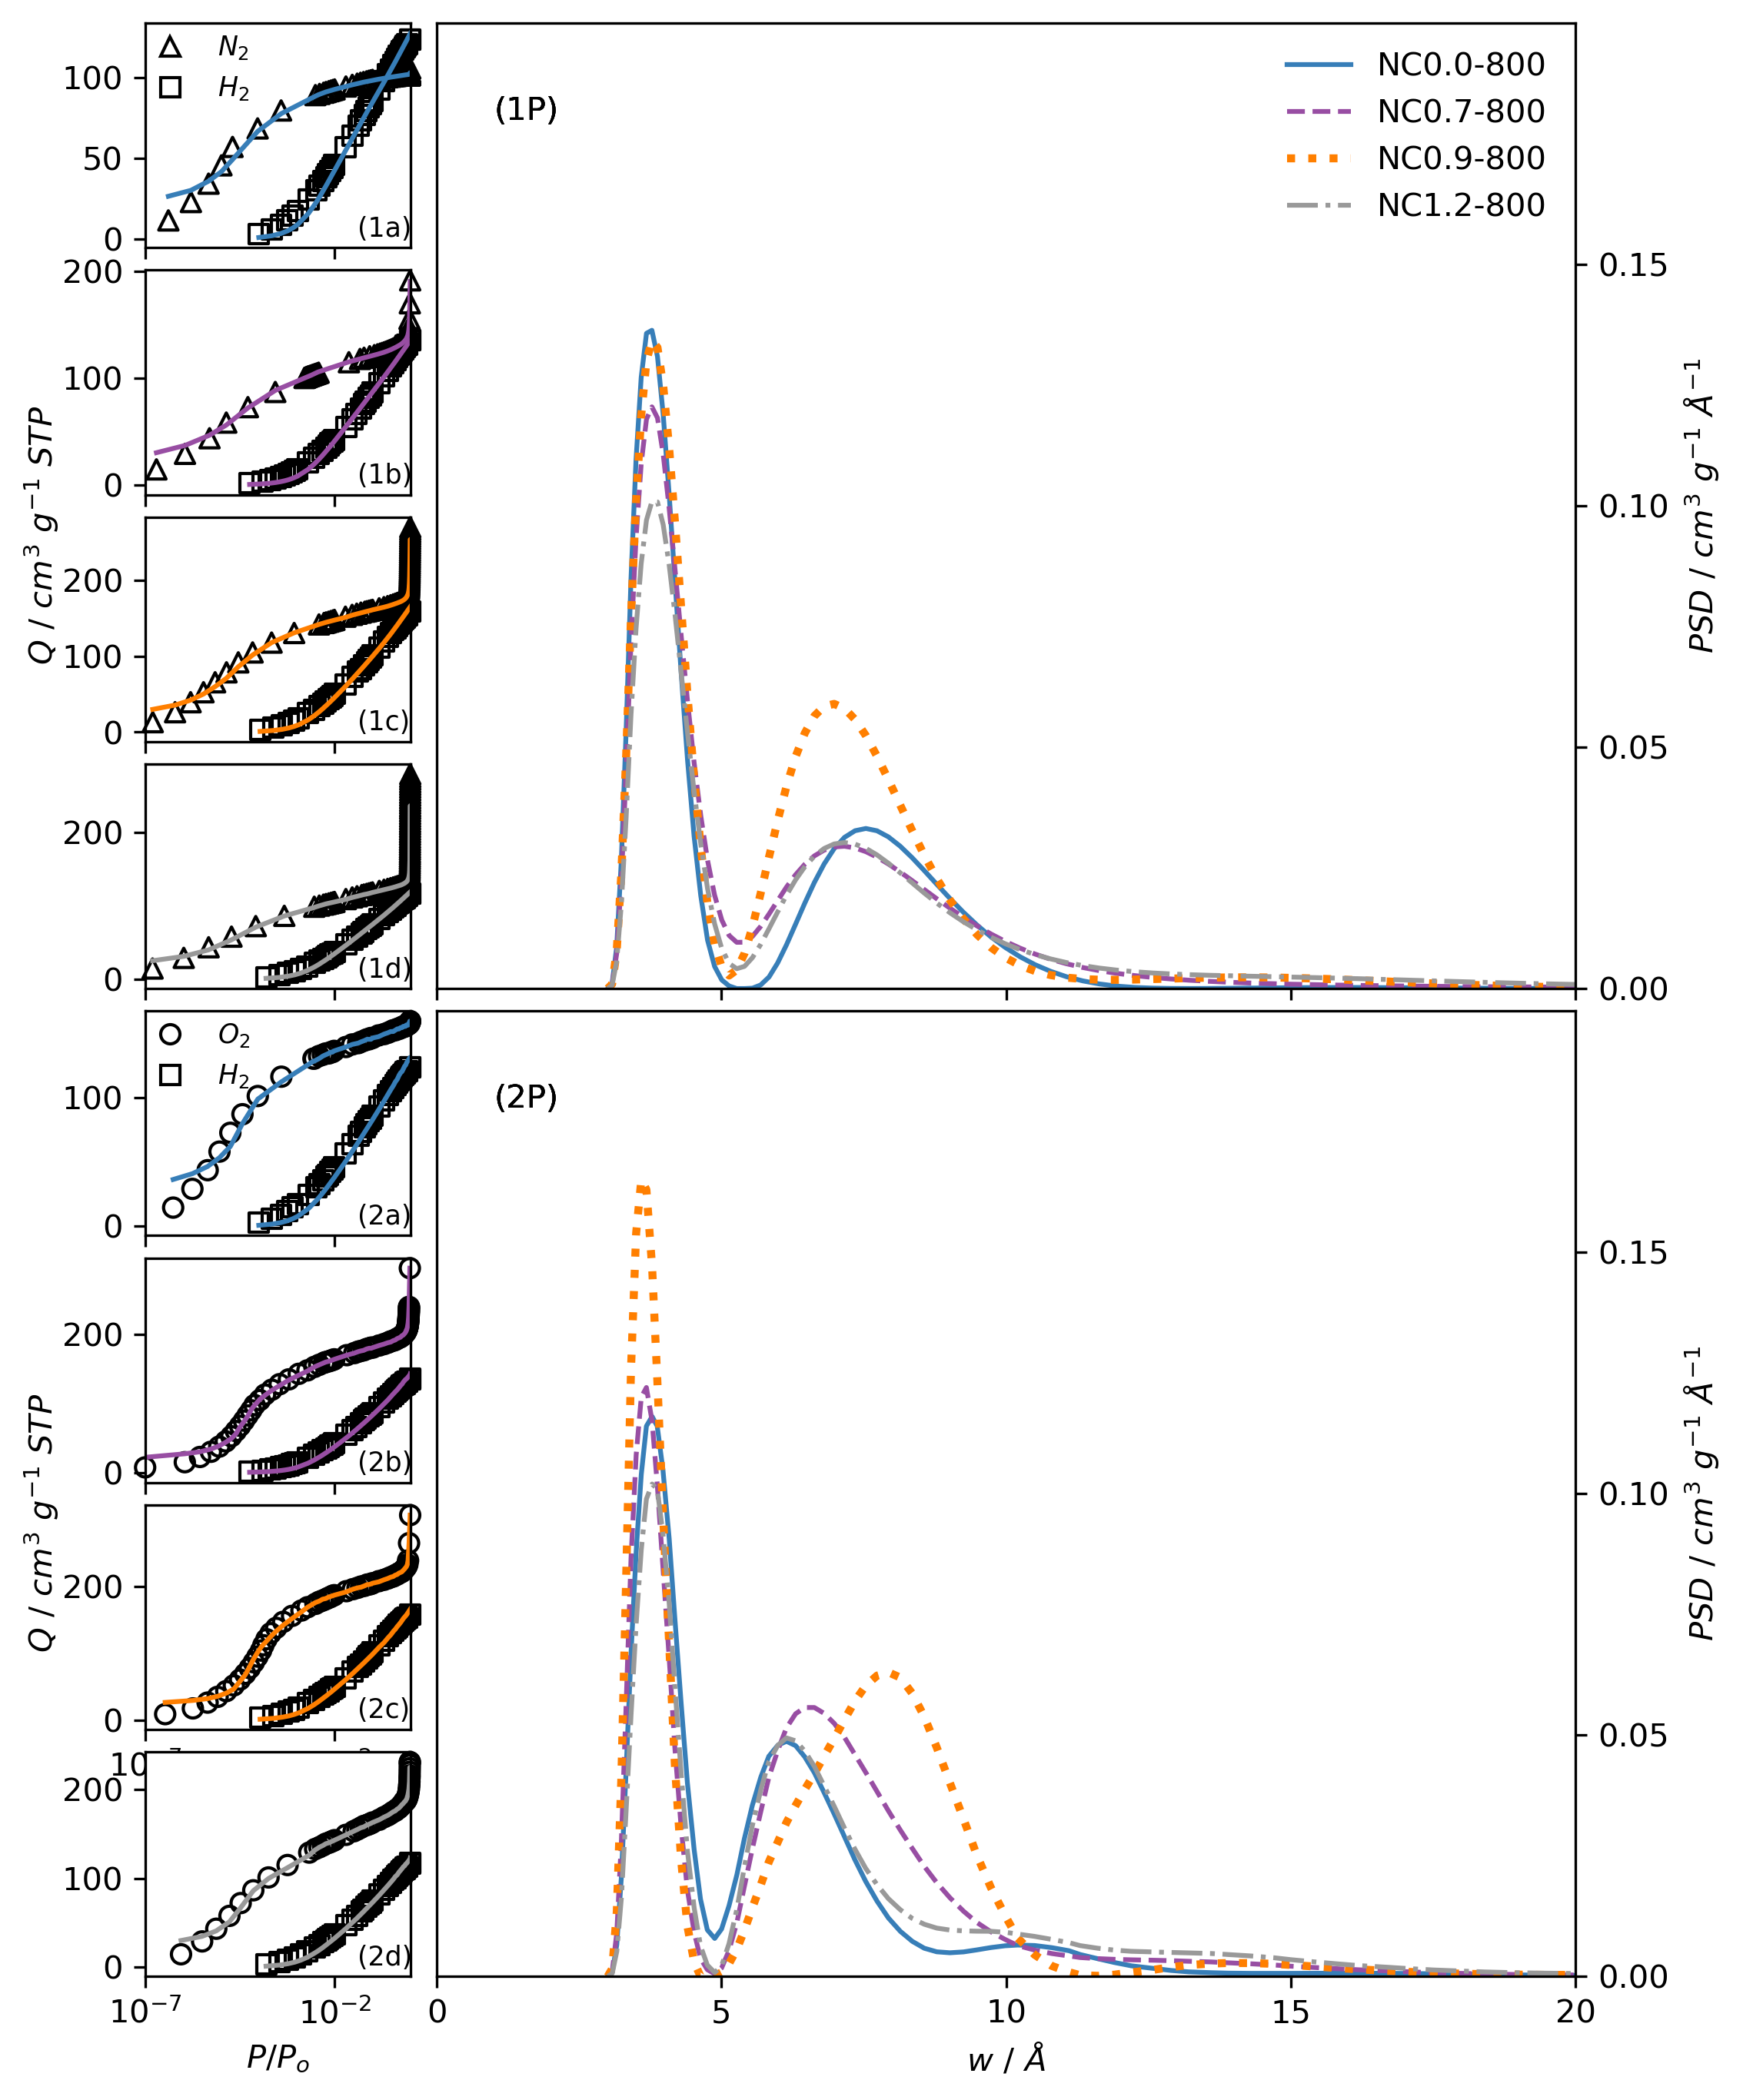
\includegraphics[width=\columnwidth,keepaspectratio]{5-dual_isotherm/figs/NCdual_isopsd.png}
    \caption{Fits to \ce{N2}/\ce{H2} (1a, 1b, 1c) and \ce{O2}/\ce{H2} (2a, 2b, 2c) isotherms of samples NC\textit{x.x}-800 (for all values of \textit{x.x} from 0.0 to 1.2), and resultant \acrshortpl{psd} (1P, 2P).}
    \label{fig:NC_contraction}
\end{figure}

The analysis performed using dual \ce{N2}/\ce{H2} porosimetry (see figure \ref{fig:NC_contraction}(1P)) indicates that the reduction in porosity for NC1.2-800 is associated with a decrease in the size of the peaks in the \acrshort{psd} relative to NC0.9-800. That is, there is no significant shift in in the position of the maxima but simply a reduction in overall porosity associated with both of these maxima. This is consistent with the overall conclusion in \ref{pub:dual_iso}, in that \ce{N2}/\ce{H2} analysis doesn't show variation in pore widths with degree of activation. On the other hand, \ce{O2}/\ce{H2} analysis (see figure \ref{fig:NC_contraction}(2P)) shows a contraction in the breadth of the \acrshort{psd} for \textit{x.x} of 1.2. Indeed, the position of the second maximum is the same as that for NC0.0-800. 

In section \ref{ss:NC} it was suggested that the trends in porosity were a result of competitive pore forming processes; while pore formation was dominated by formation of cross-links at \acrshort{ds} of 0.7 and 0.9, oxidative chemical activation began to take on a larger role at \acrshort{ds} of 1.2. In the case of NC0.0-800, no cross-link formation can occur thus porosity is formed \textit{via} gasification. The contraction in \acrshort{psd} for NC1.2-800 shown by \ce{O2}/\ce{H2} analysis indicates that this higher quantity of \ce{Na} present during \gls{pyrolysis} results in the destruction of cross-links and thus of the broader pores that are associated with their formation. The porosity that remains is that formed solely \textit{via} gasification as present in the \ce{Na}-free samples. On the other hand, the information given by \ce{N2}/\ce{H2} analysis indicates that there is a loss in porosity that is much more mechanistically difficult to explain. Perhaps the reduction in size of the second maximum could simply be put down to of pore collapse \textit{via} overactivation, but this ought to be associated with much more significant increase in mesoporosity which is not present here. It is much more difficult to derive nuanced, logical hypotheses on these pore formation mechanisms from the \ce{N2}/\ce{H2} analysis.

\section{Summary \& future work}
Porosimetry performed using \ce{O2} shows promise in more accurate determination of \acrshort{psd}, and porosity in general in ultramicroporous carbons. In particular, simultaneous fitting of the respective 2D-NLDFT-HS kernel to \ce{O2} and \ce{H2} isotherms consistently reveals a bimodal \acrshort{psd}. While this is also present for dual fits to \ce{N2} and \ce{H2}, the \ce{O2}/\ce{H2} method seems to show broadening in the \acrshort{psd} with increasing degree of activation which is not present in analysis performed using the former pair. These results ought to inform the selection of porosimetric \glspl{adsorbate} for highly ultramicroporous carbons. Furthermore, the results from dual isotherm analyses give further insights into potential mechanistic details of the somewhat unusual pore formation mechanisms in the \glspl{turbostratic carbon} reported in chapter \ref{ch:impregnation}. 

There was an attempt to fit three isotherms (\ce{N2}, \ce{O2}, and \ce{H2}) to their respective 2D-NLDFT-HS kernels simultaneously which proved fruitless. This gave poor fits to the experimental data, especially for carbons with a low degree of activation. This may indicate the difficulty \ce{N2} has in penetrating the smallest of \glspl{ultramicropore} and thus its limited utility in measuring porosity at these pore widths. However, three-way fits may indeed prove to be useful in the future in particular for materials with greater \acrshort{psd} hierarchy. For example, a simultaneous fit to \ce{SF6}, \ce{O2} and \ce{H2} isotherms (at \qtylist[list-units=single]{-50;-196;-196}{\degreeCelsius} respectively) would minimise the overlap of accessible pores for each of the three \glspl{adsorbate}, as the $d_k$ is \qty{5.50}{\angstrom}, so excludes the smallest of \glspl{ultramicropore}. This analysis may however not be necessary and the same information could be gleaned by using \ce{SF6} and \ce{H2}, which would minimise the overlap of pore sizes accessible to both \glspl{adsorbate} In addition, \ce{SF6} has a zero quadrupole moment compared to \ce{O2}'s of 0.155 which ought to reduce errors produced by carbon surface heterogeneity.


\newpage
\section[Publication I Supporting Information]{Publication I Supporting Information: Confirmation of pore formation mechanisms in biochars and activated carbons by dual isotherm analysis}

\textbf{Contribution of the author}: The author performed all synthesis and instrumental analysis of samples in the work, analysed the results and wrote the manuscript.

\textbf{Note}: For this publication, the sample names are slightly different. The variable \textit{x.xx} in SA\textit{x.xx-HHH} samples is truncated to \textit{x.x}, i.e. SA0.5-250 in the publication is equivalent to SA0.50-250 in chapter \ref{ch:impregnation}. As for NC\textit{x.x-TTT} samples only samples with \textit{TTT} of \qty{800}{\degreeCelsius} are examined, thus NC0.9 is identical to NC0.9-800 in chapter \ref{ch:impregnation}.
\setcounter{opagenum}{\thepage}
\newpage

\setlength{\originalVOffset}{\voffset}   
\setlength{\originalHOffset}{\hoffset}

\setlength{\voffset}{0cm}
\setlength{\hoffset}{0cm}
% too big for overleaf, try compilation later.

\includepdf[pagecommand={
    \setcounter{page}{\theopagenum}
    \thispagestyle{empty}
    },
    pages=-]{5-dual_isotherm/si_02.pdf}
\setlength{\voffset}{\originalVOffset}
\setlength{\hoffset}{\originalHOffset}

\bibliographystyle{rsc}
\bibliography{bibliography/bib}
\chapter{python Porosity Uptake Correlator (pyPUC)}
\label{ch:pyPUC}

\section{Introduction}

\section{Rationale for pyPUC}
\subsection{Dual isotherm analyses and relationship to low-pressure \ce{CO2} uptake}

\section{Software Design}

\newpage
\section[Publication III]{Publication III: Brute force determination of the optimum pore sizes for
\ce{CO2} uptake}

\textbf{Contribution of the author}: The author came up with the concept of the pyPUC software, designed and implemented it, and performed all analyses. A portion of the experimental work necessary to create DataSet 1, and all experimental work for DataSet 2 was also done by the author. The author wrote the paper in its entirety.

\newpage

\setlength{\originalVOffset}{\voffset}   
\setlength{\originalHOffset}{\hoffset}

\setlength{\voffset}{0cm}
\setlength{\hoffset}{0cm}
% too big for overleaf, try compilation later.
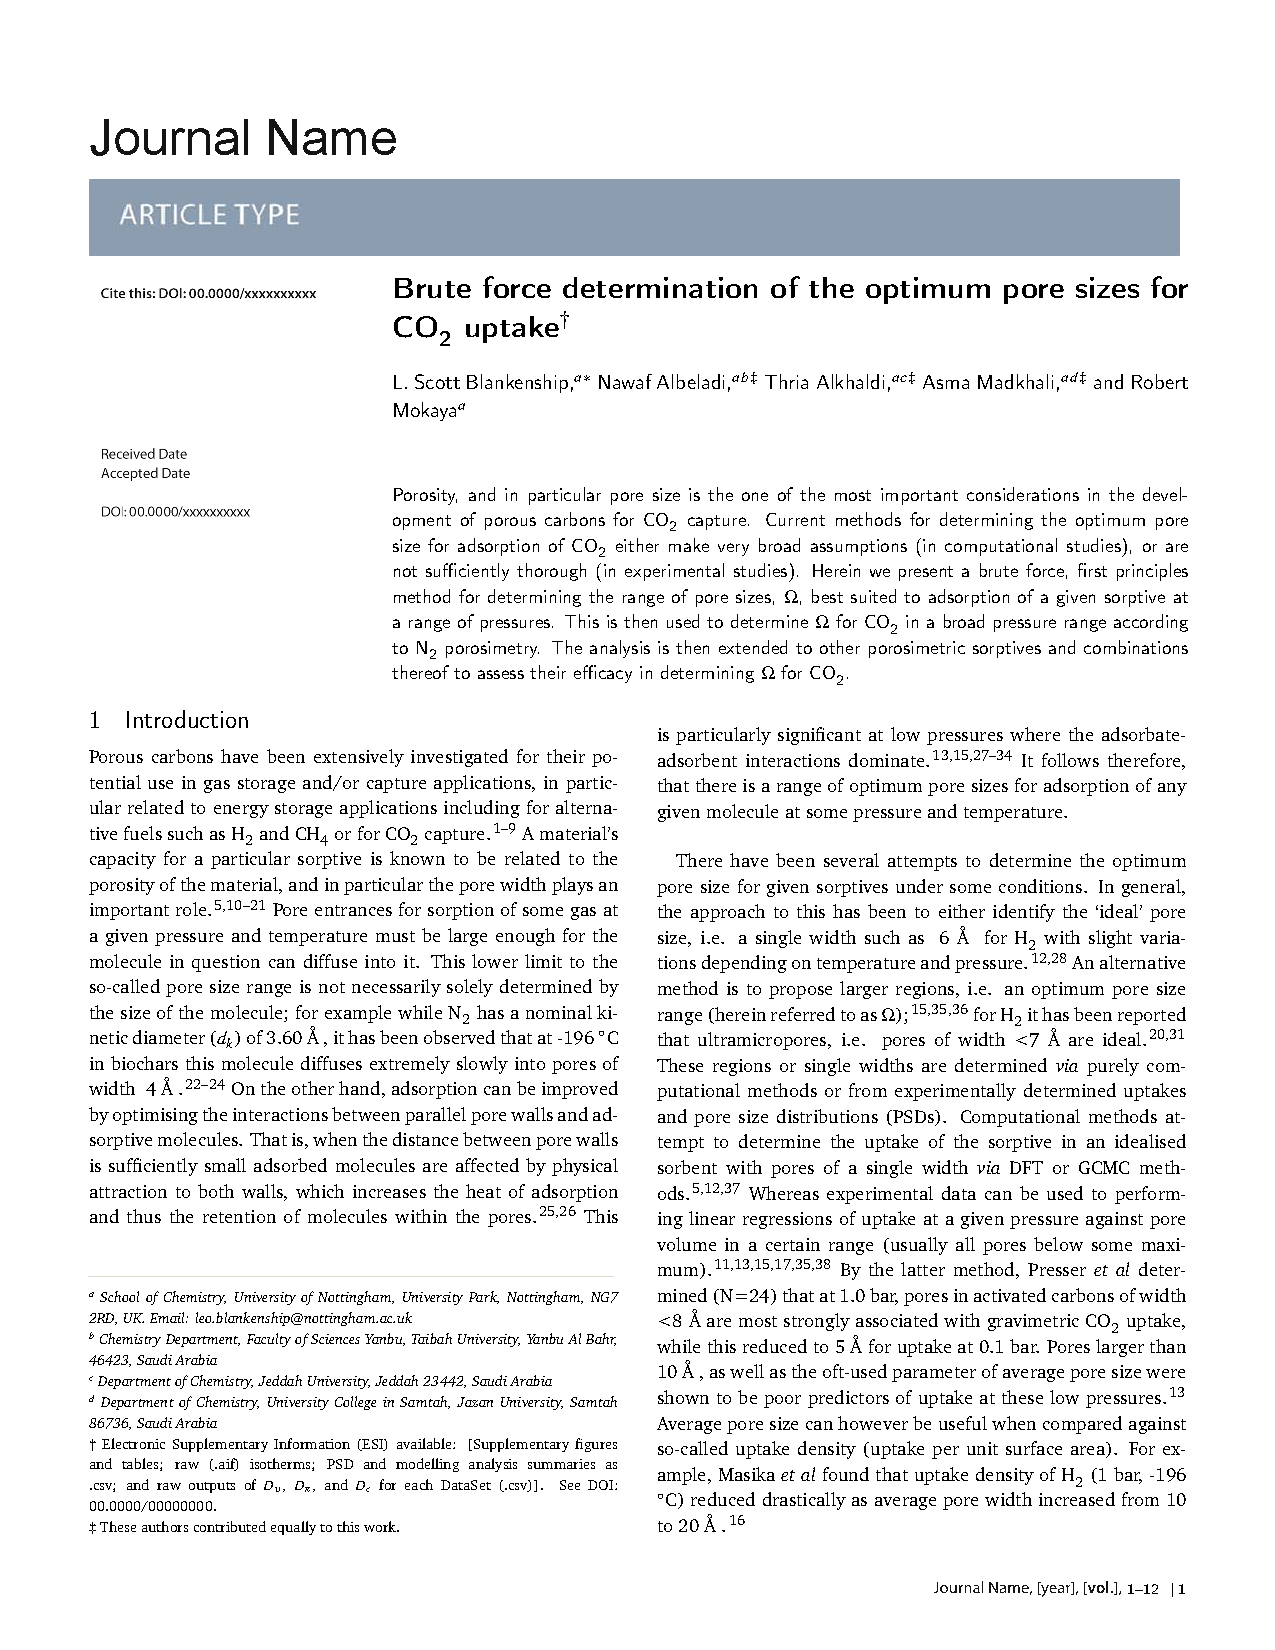
\includepdf[pages=-]{publication_03}
\setlength{\voffset}{\originalVOffset}
\setlength{\hoffset}{\originalHOffset}

\section{Summary \& Future Work}

\newpage
\section[Publication III Supporting Information]{Publication III Supporting Information: Brute force determination of the optimum pore sizes for \ce{CO2} uptake}

\newpage

\setlength{\originalVOffset}{\voffset}   
\setlength{\originalHOffset}{\hoffset}

\setlength{\voffset}{0cm}
\setlength{\hoffset}{0cm}
% too big for overleaf, try compilation later.
%\includepdf[pages=-]{si_03}
\setlength{\voffset}{\originalVOffset}
\setlength{\hoffset}{\originalHOffset}

\section*{References}
\chapter{Conclusions \& Outlook}
\label{ch:conclusion}
The work detailed in this thesis investigated the synthesis of \glspl{turbostratic carbon} to be utilised for \ce{CO2} capture, firstly developing the understanding of carbons derived from \acrfullpl{ucf} (see chapter \ref{ch:cbs}) based on the authors previous work detailed in \ref{pub:CA} and \ref{pub:CB}. It was found that the removal of the wrapping paper on the \acrfull{ucf} is likely an essential step in the production of carbons with the extremely high porosities \textit{via} activation using \ce{KOH}, and associated gravimetric \ce{H2} capacities seen in \ref{pub:CB}. Furthermore, retaining the wrapping paper in the precursor resulted in high levels of irremovable inorganic material left in the derived \glspl{turbostratic carbon}. The resultant hierarchically porous, medium surface area carbons were found to have reasonable \ce{CO2} uptake capacity nonetheless and such materials may have further application in \acrfull{psa} applications. In addition, a series of carbons activated without the use of any external \gls{porogen} were produced, and these materials \textit{appear} to be highly ultramicroporous, though the analytic techniques used in the chapter are insufficient to yield precise and accurate data concerning porosity within this pore width range. 

Inspired by assertions that impregnated contaminant \glspl{porogen} in \acrshortpl{ucf} may provide a degree of porosity that is higher than expected from \ce{KOH} activation alone, in chapter \ref{ch:impregnation} this so-called impregnation technique was further explored. This was done \textit{via} the hydrothermal impregnation of \ce{KOH} into \acrfull{sd} prior to pyrolytic \gls{activation}, as well as by the pyrolysis of \acrfull{nc}. The relationship between porosity of the derived samples and their activation conditions was of great interest. In particular, highly ultramicroporous carbons can be synthesised \textit{via} both methods explored in this chapter. Such porosity previously been shown to be useful for low-pressure \ce{CO2} capture. However what is more interesting is the relationship between porosity of- and the synthetic conditions used- to form these novel carbons. In particular, while in general carbons derived from \acrshort{sd} are essentially entirely microporous, at a sufficiently high \ce{KOH}:\acrshort{sd} ratio the derived material becomes almost entirely mesoporous. This change in \acrshort{psd} is also accompanied by an large reduction in density, resulting in an unprecedentedly diffuse \gls{turbostratic carbon}. The \acrshort{nc}-derived samples showed unusual trends in the relationship between \gls{porogen}:precursor ratio and porosity, in that maximisation of porosity appears to occur for an \ce{Na}:\ce{C} atomic ratio of 1.2 (corresponding to a \acrfull{ds} of the sodium carboxymethyl group of 0.9). As the precursor is polymeric with carboxyl sidechains, it can be expected that cross-links may form at some point during synthesis thus yielding porosity independently from the oxidative action of \ce{Na} and \ce{Na}-containing compounds. The aforementioned breakdown in porosity indicates that these two pore forming processes may be competitive; at higher \ce{Na}:\ce{C} ratios oxidative chemical activation destroys porosity previously produced \textit{via} cross-link formation.

The synthesis-based chapters \ref{ch:cbs} and \ref{ch:impregnation} give way to further routes of investigation with respect to routes to microporous carbons for small molecule adsorption. In particular, the reason for the difficulty in removal of inorganic contaminants in \gls{ucf}-derived carbons ought to be further investigated, as the extensive washing steps used are common and have been found to be overwhelmingly successful in the community of researchers working on \glspl{activated carbon}. Indeed, the metals identified ought to be very water soluble. Routes to understanding the stubbornness of these species include use of other solvents to remove them, as well as in-depth electron microscopic techniques to understand if and whether the metal clusters are `stuck' inside the pores. Additionally, understanding of the mechanisms of porogenesis in the materials described in chapter \ref{ch:impregnation} ought to be fully elucidated, perhaps \textit{via} thermal kinetic studies, in situ electron microscopy, and/or analysis of volatiles released during the pyrolytic processes. 

In terms of analytical methods what is clear from both of the synthetic chapters is that the traditional method of porosimetry as derived from \ce{N2} isotherms measured at \qty{-196}{\degreeCelsius} is insufficient, in that \ce{N2} does not appear to easily diffuse into the \glspl{ultramicropore} present in many of the materials previously described. As such, chapter \ref{ch:dual_isotherm} details the investigation of alternative porosimetric probes, namely \ce{H2} and \ce{O2}. While these probe molecules have been investigated prior to this work, this chapter showed that only the simultaneous fit of the 2D-NLDFT heterogeneous surface (2D-NLDFT-HS) kernel to both isotherms was able to give a precise and reasonable description of the subtle \acrshort{psd} broadening as associated with increased \gls{porogen} concentration. This may be related to the fact that both \ce{O2} and \ce{H2} seem to have less trouble diffusing into these extremely small pores. Apart from this, \ce{H2} has been confirmed to probe porosity that, as a result of restrictive pore openings is not accessible to the larger \ce{O2} and \ce{N2} molecules. As the low pressure \gls{adsorption} of small, environmentally-relevant molecules such as \ce{CO2} is supposed to be associated with the presence of \glspl{ultramicropore}, the accurate understanding of porosity within such pores is vital and as such the work in chapter \ref{ch:dual_isotherm} ought to inform how porosity is measured in \glspl{turbostratic carbon}. In future these techniques should be exploited on a series of porous crystaline materials with varying \acrshortpl{psd}, but with significant porosity which is poorly accessible to \ce{N2} at \qty{-196}{\degreeCelsius}. Crystallographic data can then be compared to porosities determined as a result of \acrshort{nldft} kernel fitting to each of these isotherms and pairs thereof. This will give an indication of the accuracy of each of the isothermal porosimetric techniques which is not possible to achieve on the turbostratic materials studied in this work.

Chapter \ref{ch:pyPUC} seeks to thoroughly investigate the association of pore width with \ce{CO2} uptake as a function of pressure. In order to meticulously investigate this relationship, a small piece of software known as the \acrfull{pypuc} was produced. Starting with an experimental dataset of gravimetric \ce{CO2} uptake isotherms and \acrshortpl{psd} from a set of \glspl{turbostratic carbon}, pyPUC performs linear regressions between porosity of pores with some range of widths, and \ce{CO2} uptake at a given pressure. This process is repeated for all pore width ranges and all \ce{CO2} uptakes. As a result, a statistically optimal pore width range can be determined for uptake of \ce{CO2} at a given pressure. It was confirmed that the optimum pore width range broadened with increasing pressure, but this seems to be more associated with an increase in the upper limit, that is at higher pressures \ce{CO2} uptake becomes associated with larger and larger pores. However, past some pressure \glspl{ultramicropore} become insignificant to \ce{CO2} uptake. As mentioned in the previous paragraph, \ce{N2} porosimetry is inadequate for probing the smallest of \glspl{ultramicropore}. \acrshort{pypuc} was also able to determine that the understanding of the relationship between low-pressure \ce{CO2} uptake and ultramicroporosity is best described using dual isotherm \ce{O2}/\ce{H2} porosimetry. That is, the $r^2$ values for correlations between uptake of \ce{CO2} at $\sim$1 bar or less and the optimum pore size range are best using this porosimetric method. \acrshort{pypuc} has much more potential, in particular for the investigation of the poorly understood relationship between \ce{CH4} adsorption and pore size. In addition, the software can easily be adapted to incorporate other variables such as surface chemistry and heat of \gls{adsorption} into the understandings of the relationships determined.

In summary, this thesis presents multiple novel methods for the production of highly ultramicroporous \glspl{turbostratic carbon}, and investigates improvements to the porosimetric methodology used in their characterisation. Furthermore, a computational tool (\acrshort{pypuc}) has been created, which has helped in the thorough elucidation of the relationship between \ce{CO2} uptake and pore size. This work raises interesting questions as to the nature of pore formation mechanisms in these materials, while \acrshort{pypuc} should provide a means and philosophy by which to investigate the adsorption capacity-porosity relationship in porous materials in general.


%\newpage
%\frontpagestyle
%\addcontentsline{toc}{chapter}{Bibliography}
%\bibliographystyle{apalike}
%\renewcommand\bibname{Bibliography}
%\bibliography{bibliography/bibliography}

\begin{appendices}
\addtocontents{toc}{\protect\renewcommand{\protect\cftchappresnum}{Appendix }}

\chapter{Composition}

\newpage
\begin{figure}[h]
    \centering
    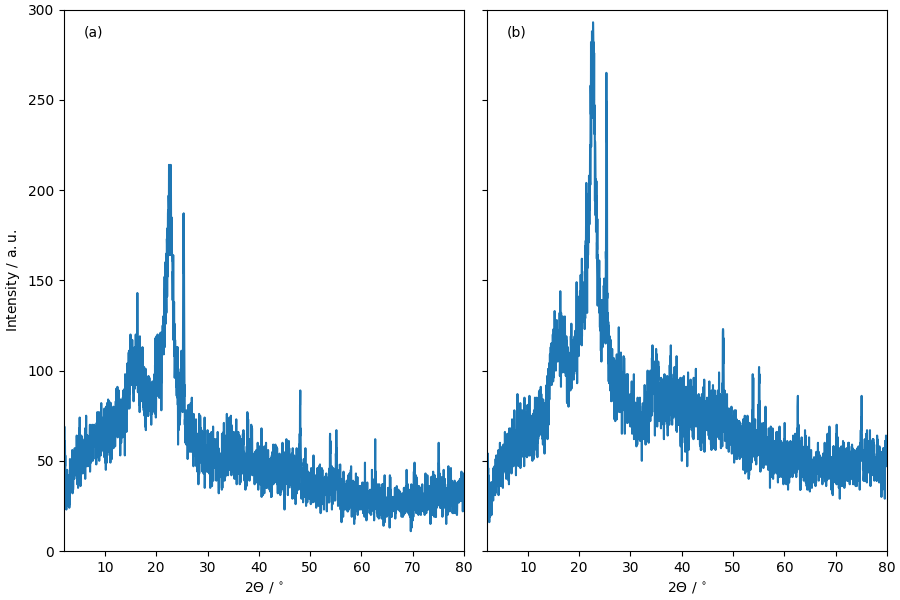
\includegraphics[width=\columnwidth, keepaspectratio]{4-cbs/figs/xrd_hydrochar.png}
    \caption{P-XRD spectra for samples hC-hydrochar (a) and hD-hydrochar (b).}
    \label{fig:xrd_hydrochar}
\end{figure}

\begin{figure}[h]
    \centering
    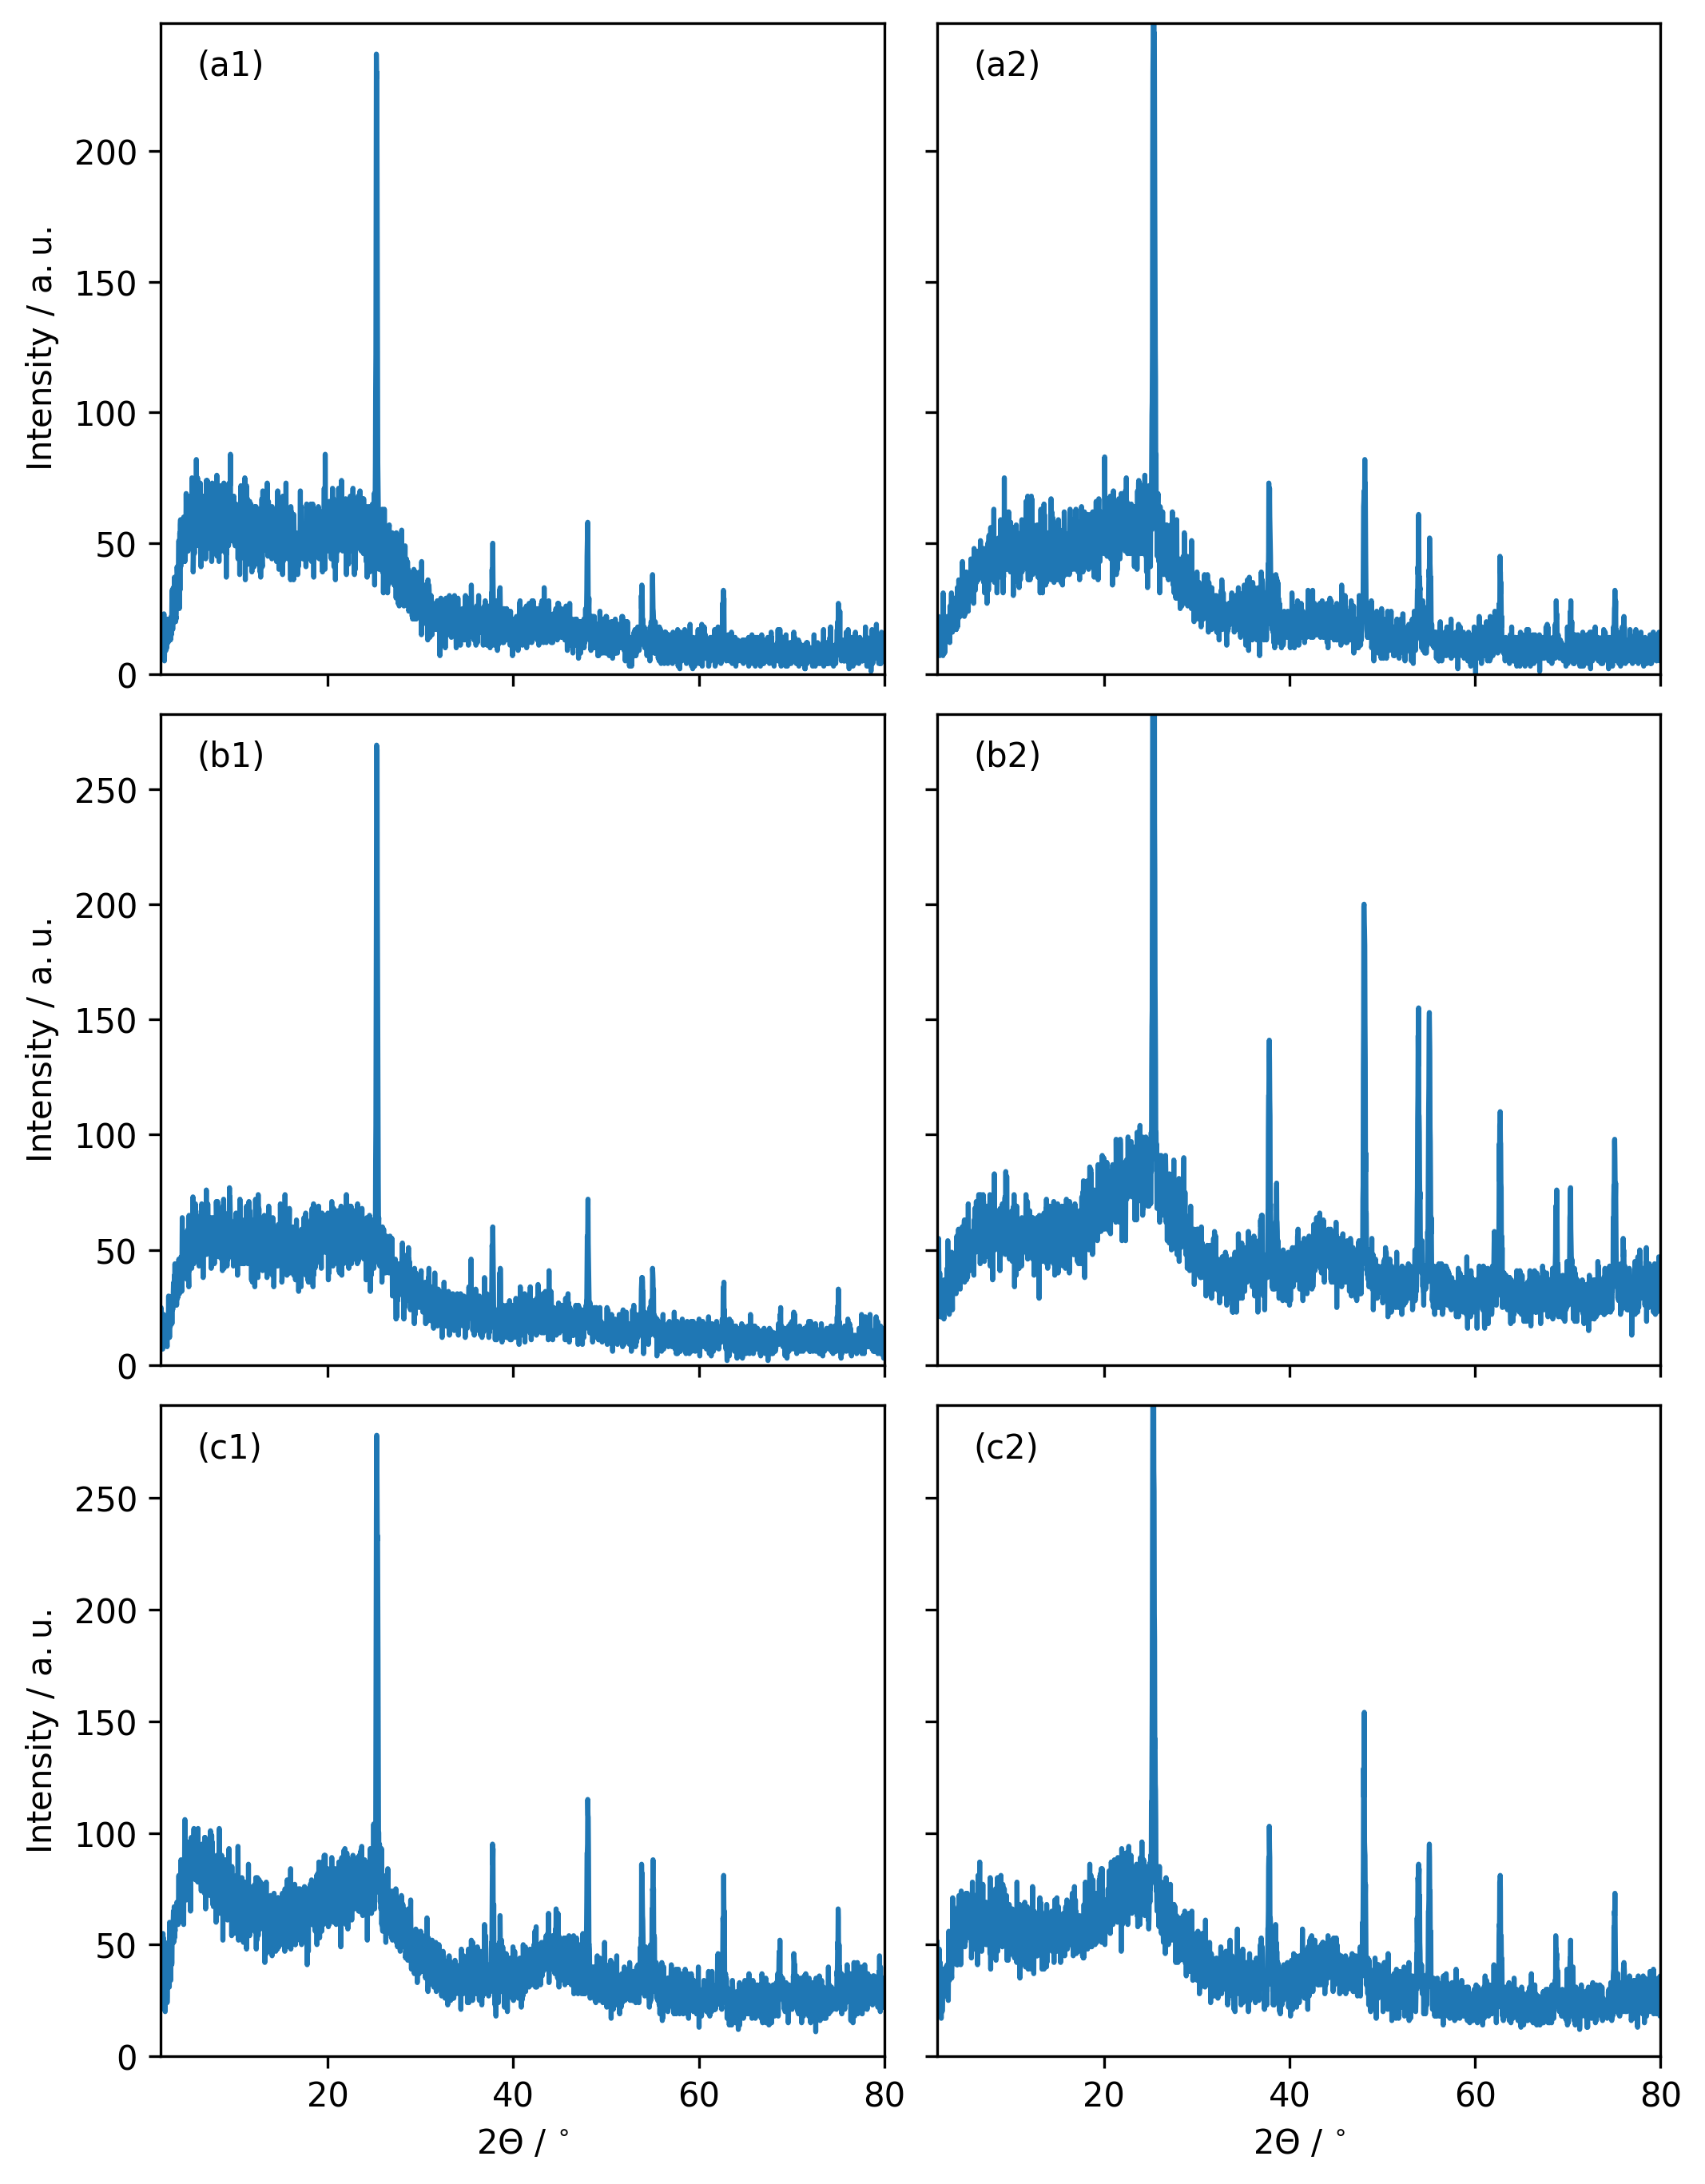
\includegraphics[width=\columnwidth, keepaspectratio]{4-cbs/figs/xrd_hC-0TTT.png}
    \caption{P-XRD spectra for samples hC-0600 (a1), hC-0600$'$ (a2), hC-0700 (b1), hC-0700$'$ (b2), hC-0800 (c1), hC-0800$'$ (c2).}
    \label{fig:xrd_hC-0TTT}
\end{figure}

\begin{figure}[h]
    \centering
    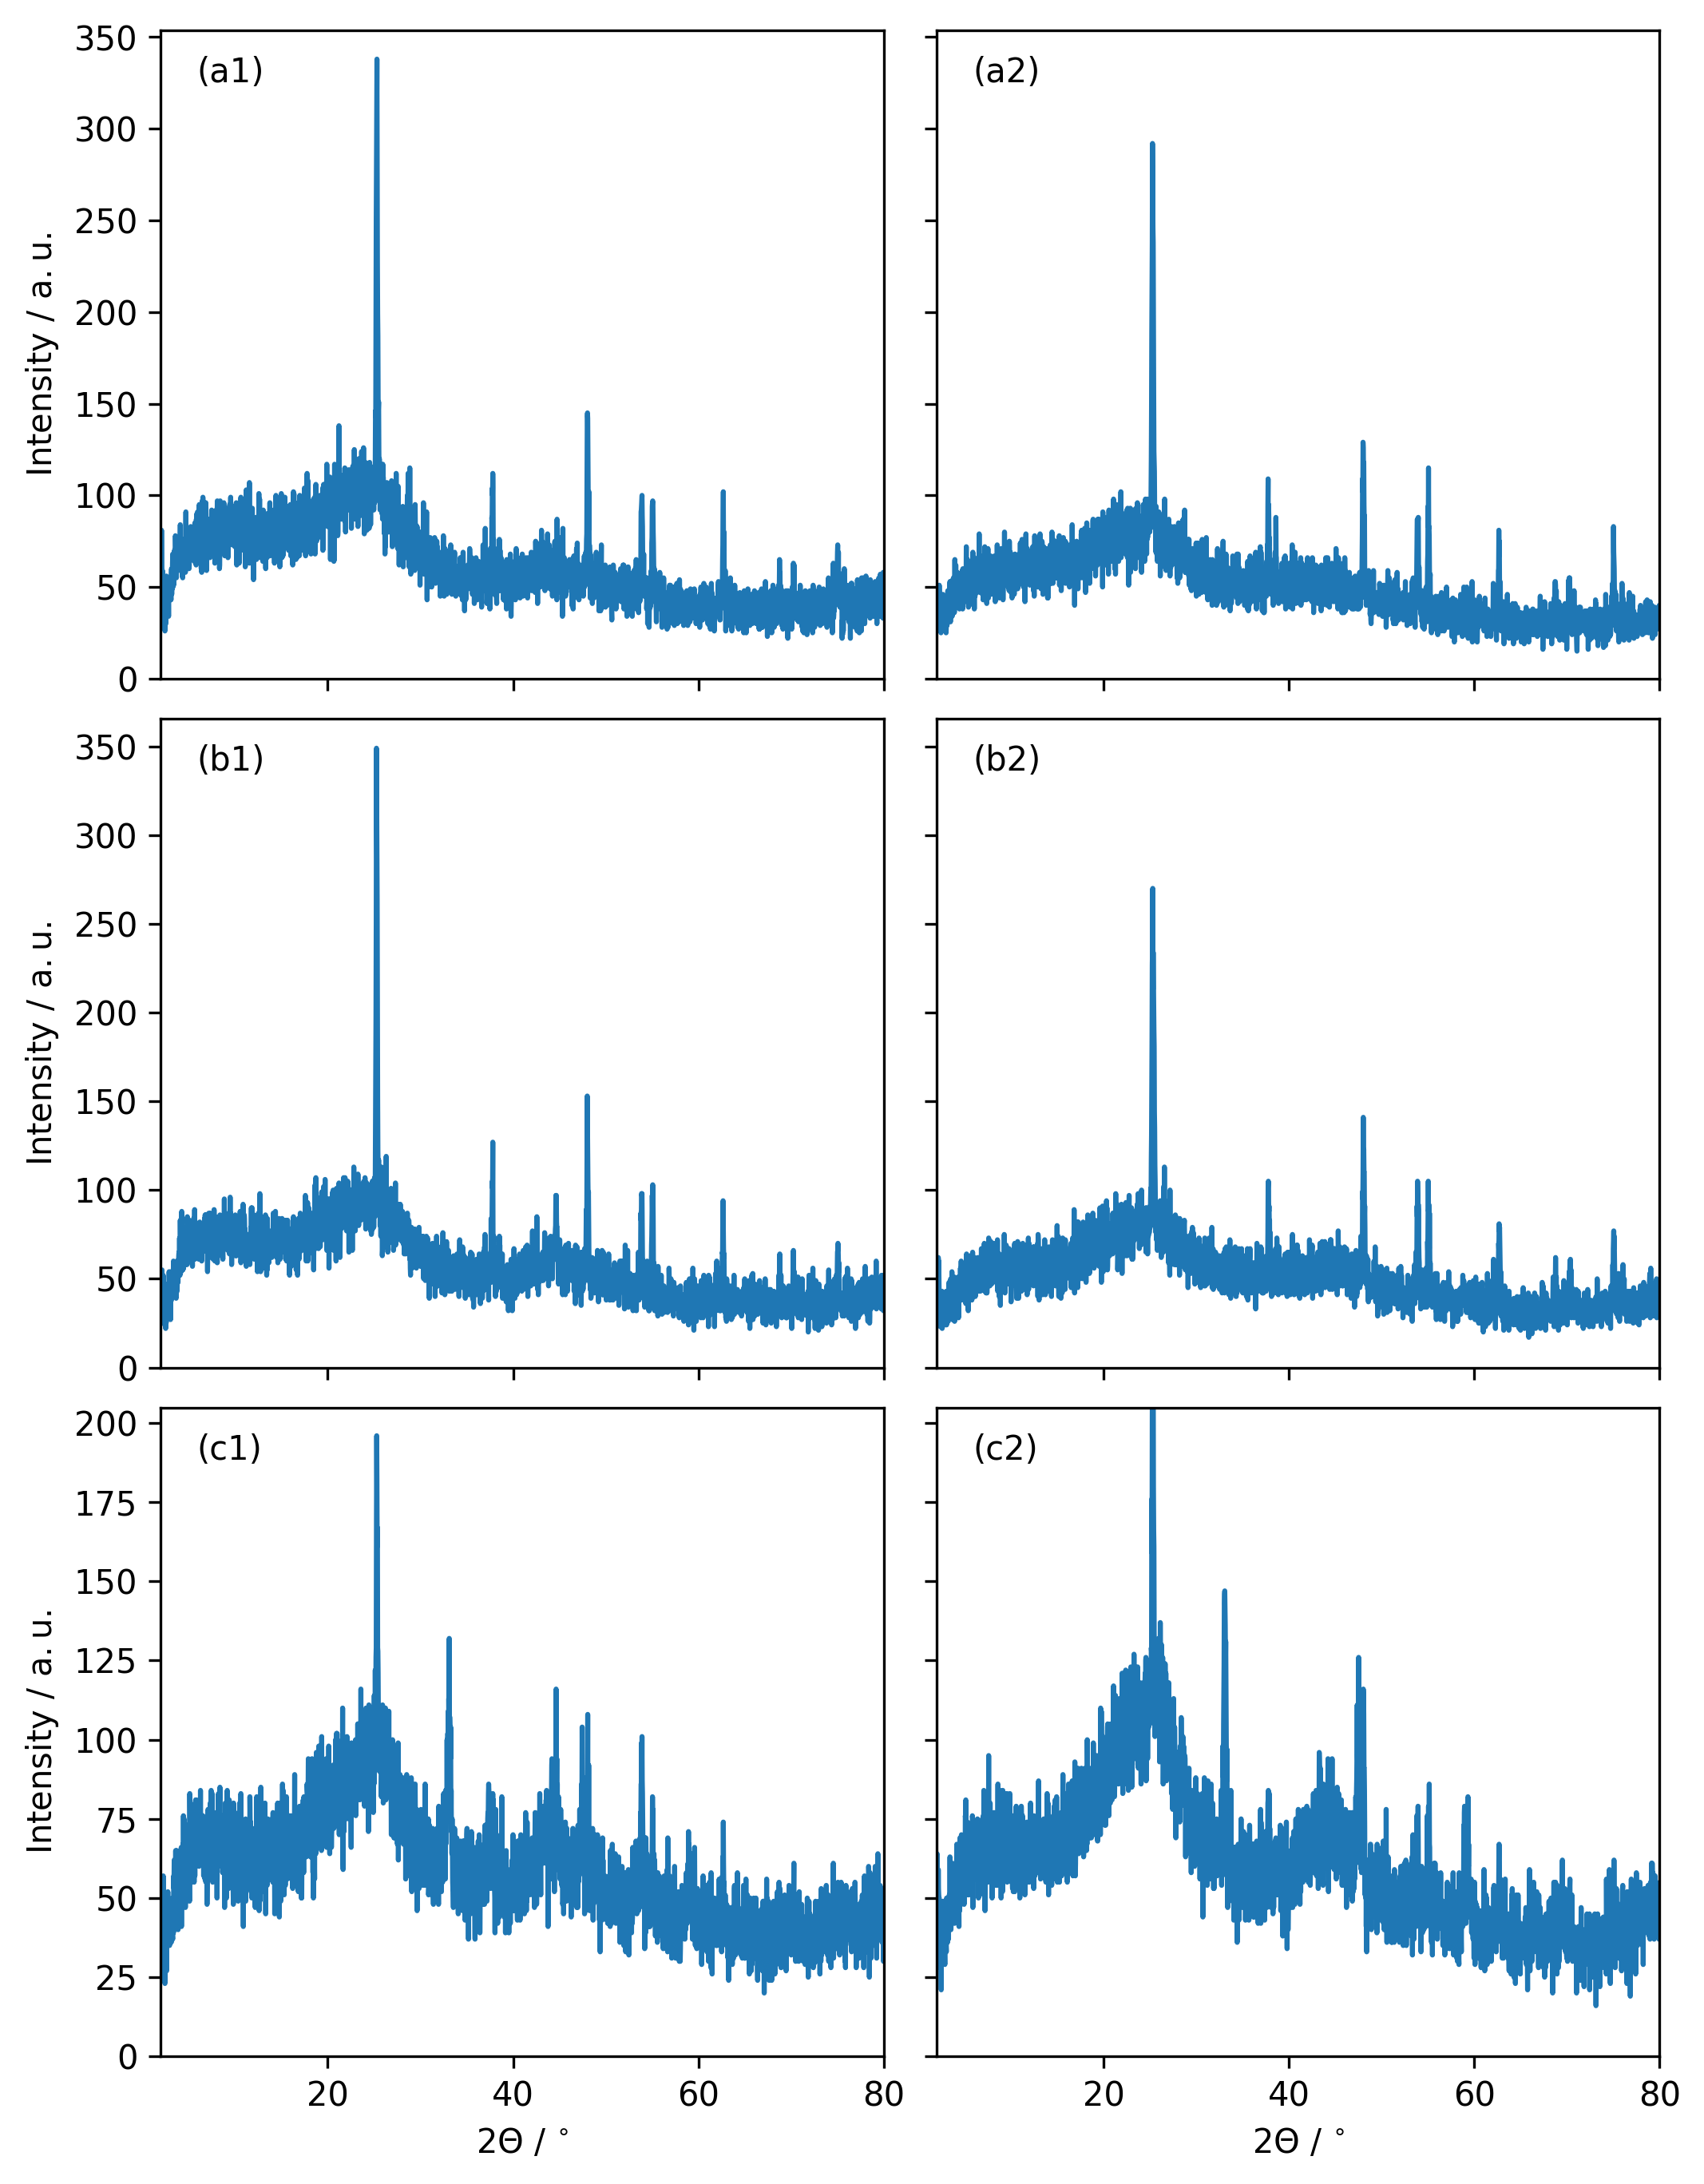
\includegraphics[width=\columnwidth, keepaspectratio]{4-cbs/figs/xrd_hD-0TTT.png}
    \caption{P-XRD spectra for samples hD-0600 (a1), hD-0600$'$ (a2), hD-0700 (b1), hD-0700$'$ (b2), hD-0800 (c1), hD-0800$'$ (c2).}
    \label{fig:xrd_hD-0TTT}
\end{figure}

\begin{figure}[h]
    \centering
    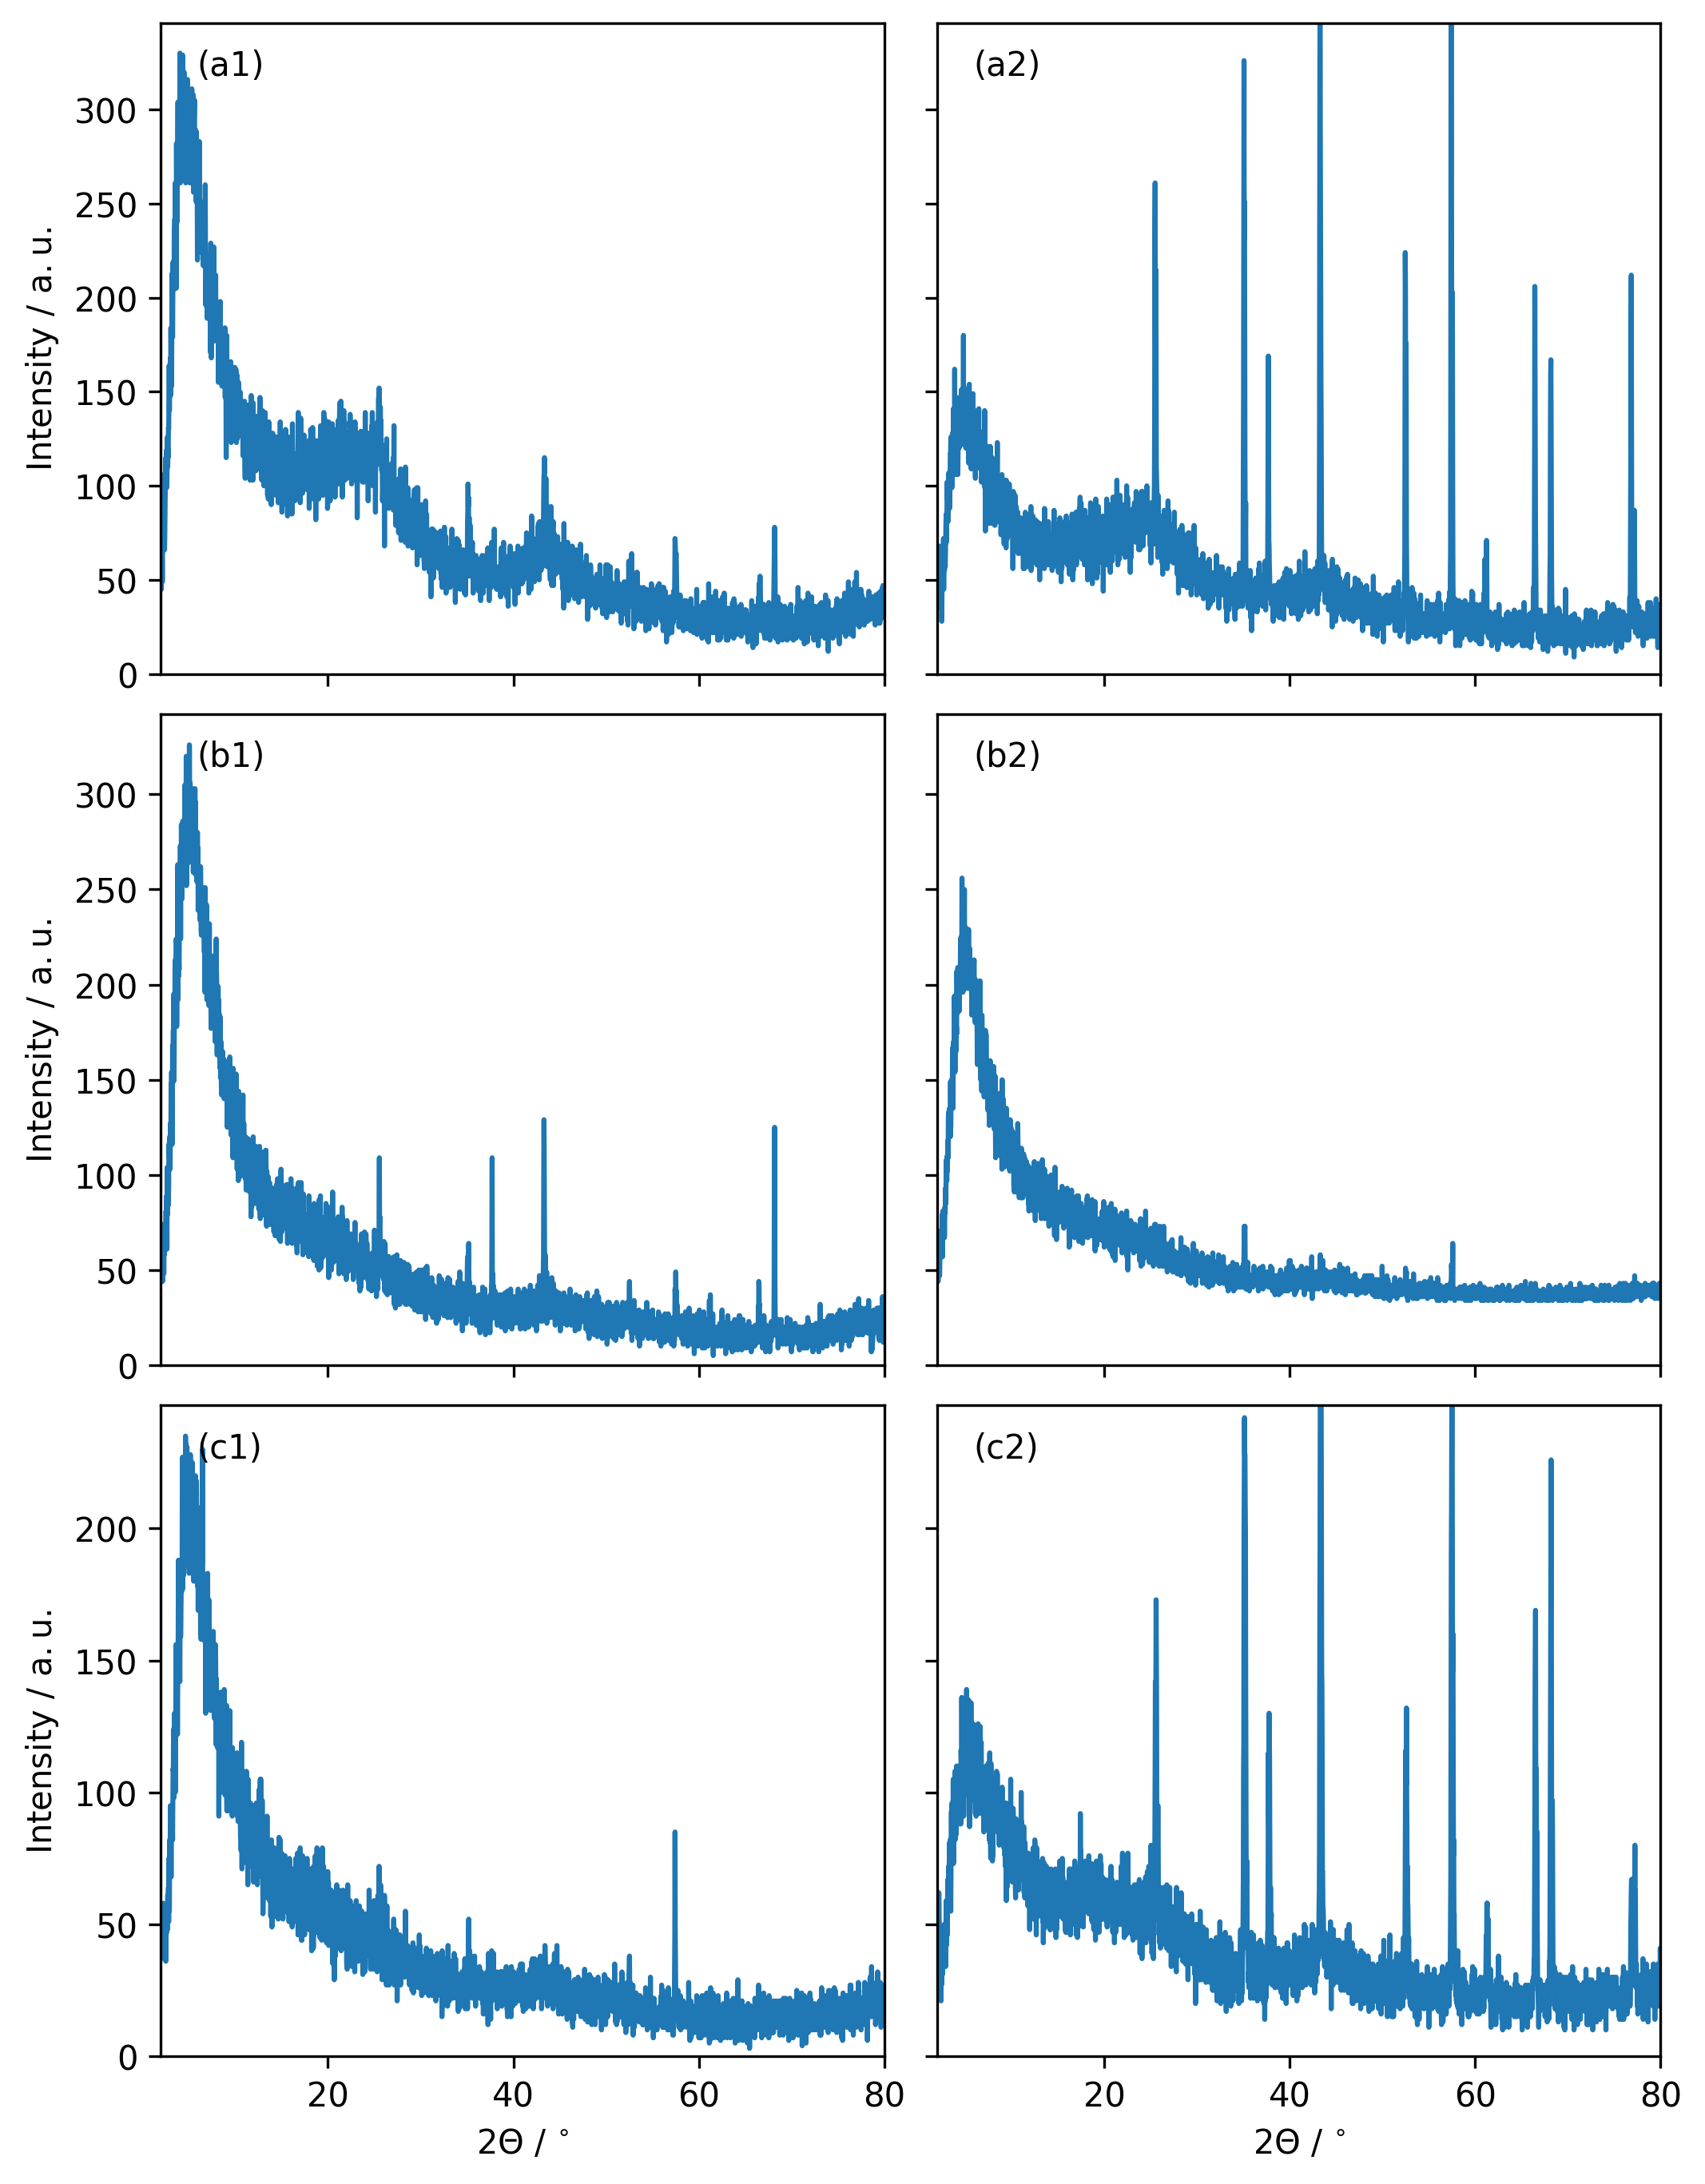
\includegraphics[width=\columnwidth, keepaspectratio]{4-cbs/figs/xrd_KOH.png}
    \caption{P-XRD spectra for samples hC-4600 (a1), hD-4600 (a2), hC-4700 (b1), hD-4700 (b2), hC-4800 (c1), hD-4800 (c2).}
    \label{fig:xrd_KOH}
\end{figure}

\begin{figure}[h]
    \centering
    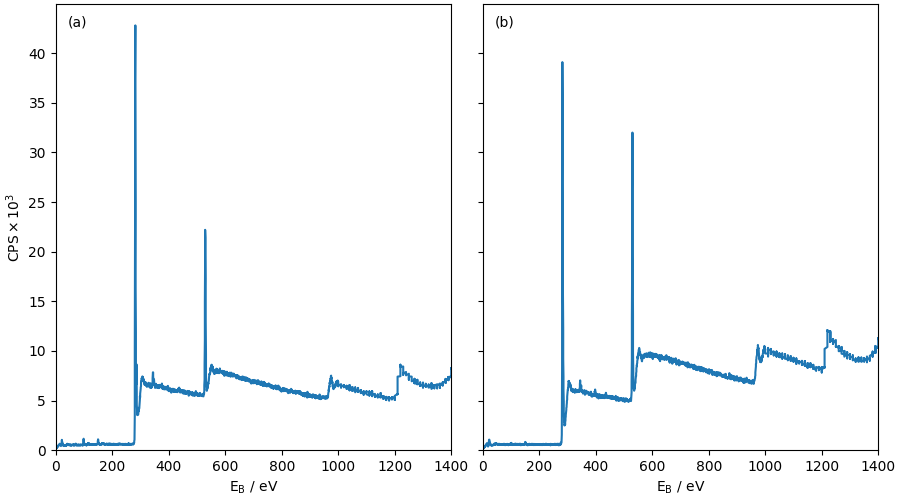
\includegraphics[width=\columnwidth, keepaspectratio]{4-cbs/figs/xps.png}
    \caption{XPS spectra for samples hD-0700 (a) and hD-hydrochar (b).}
    \label{fig:cb_xps}
\end{figure}

\begin{figure}[h!]
    \centering
    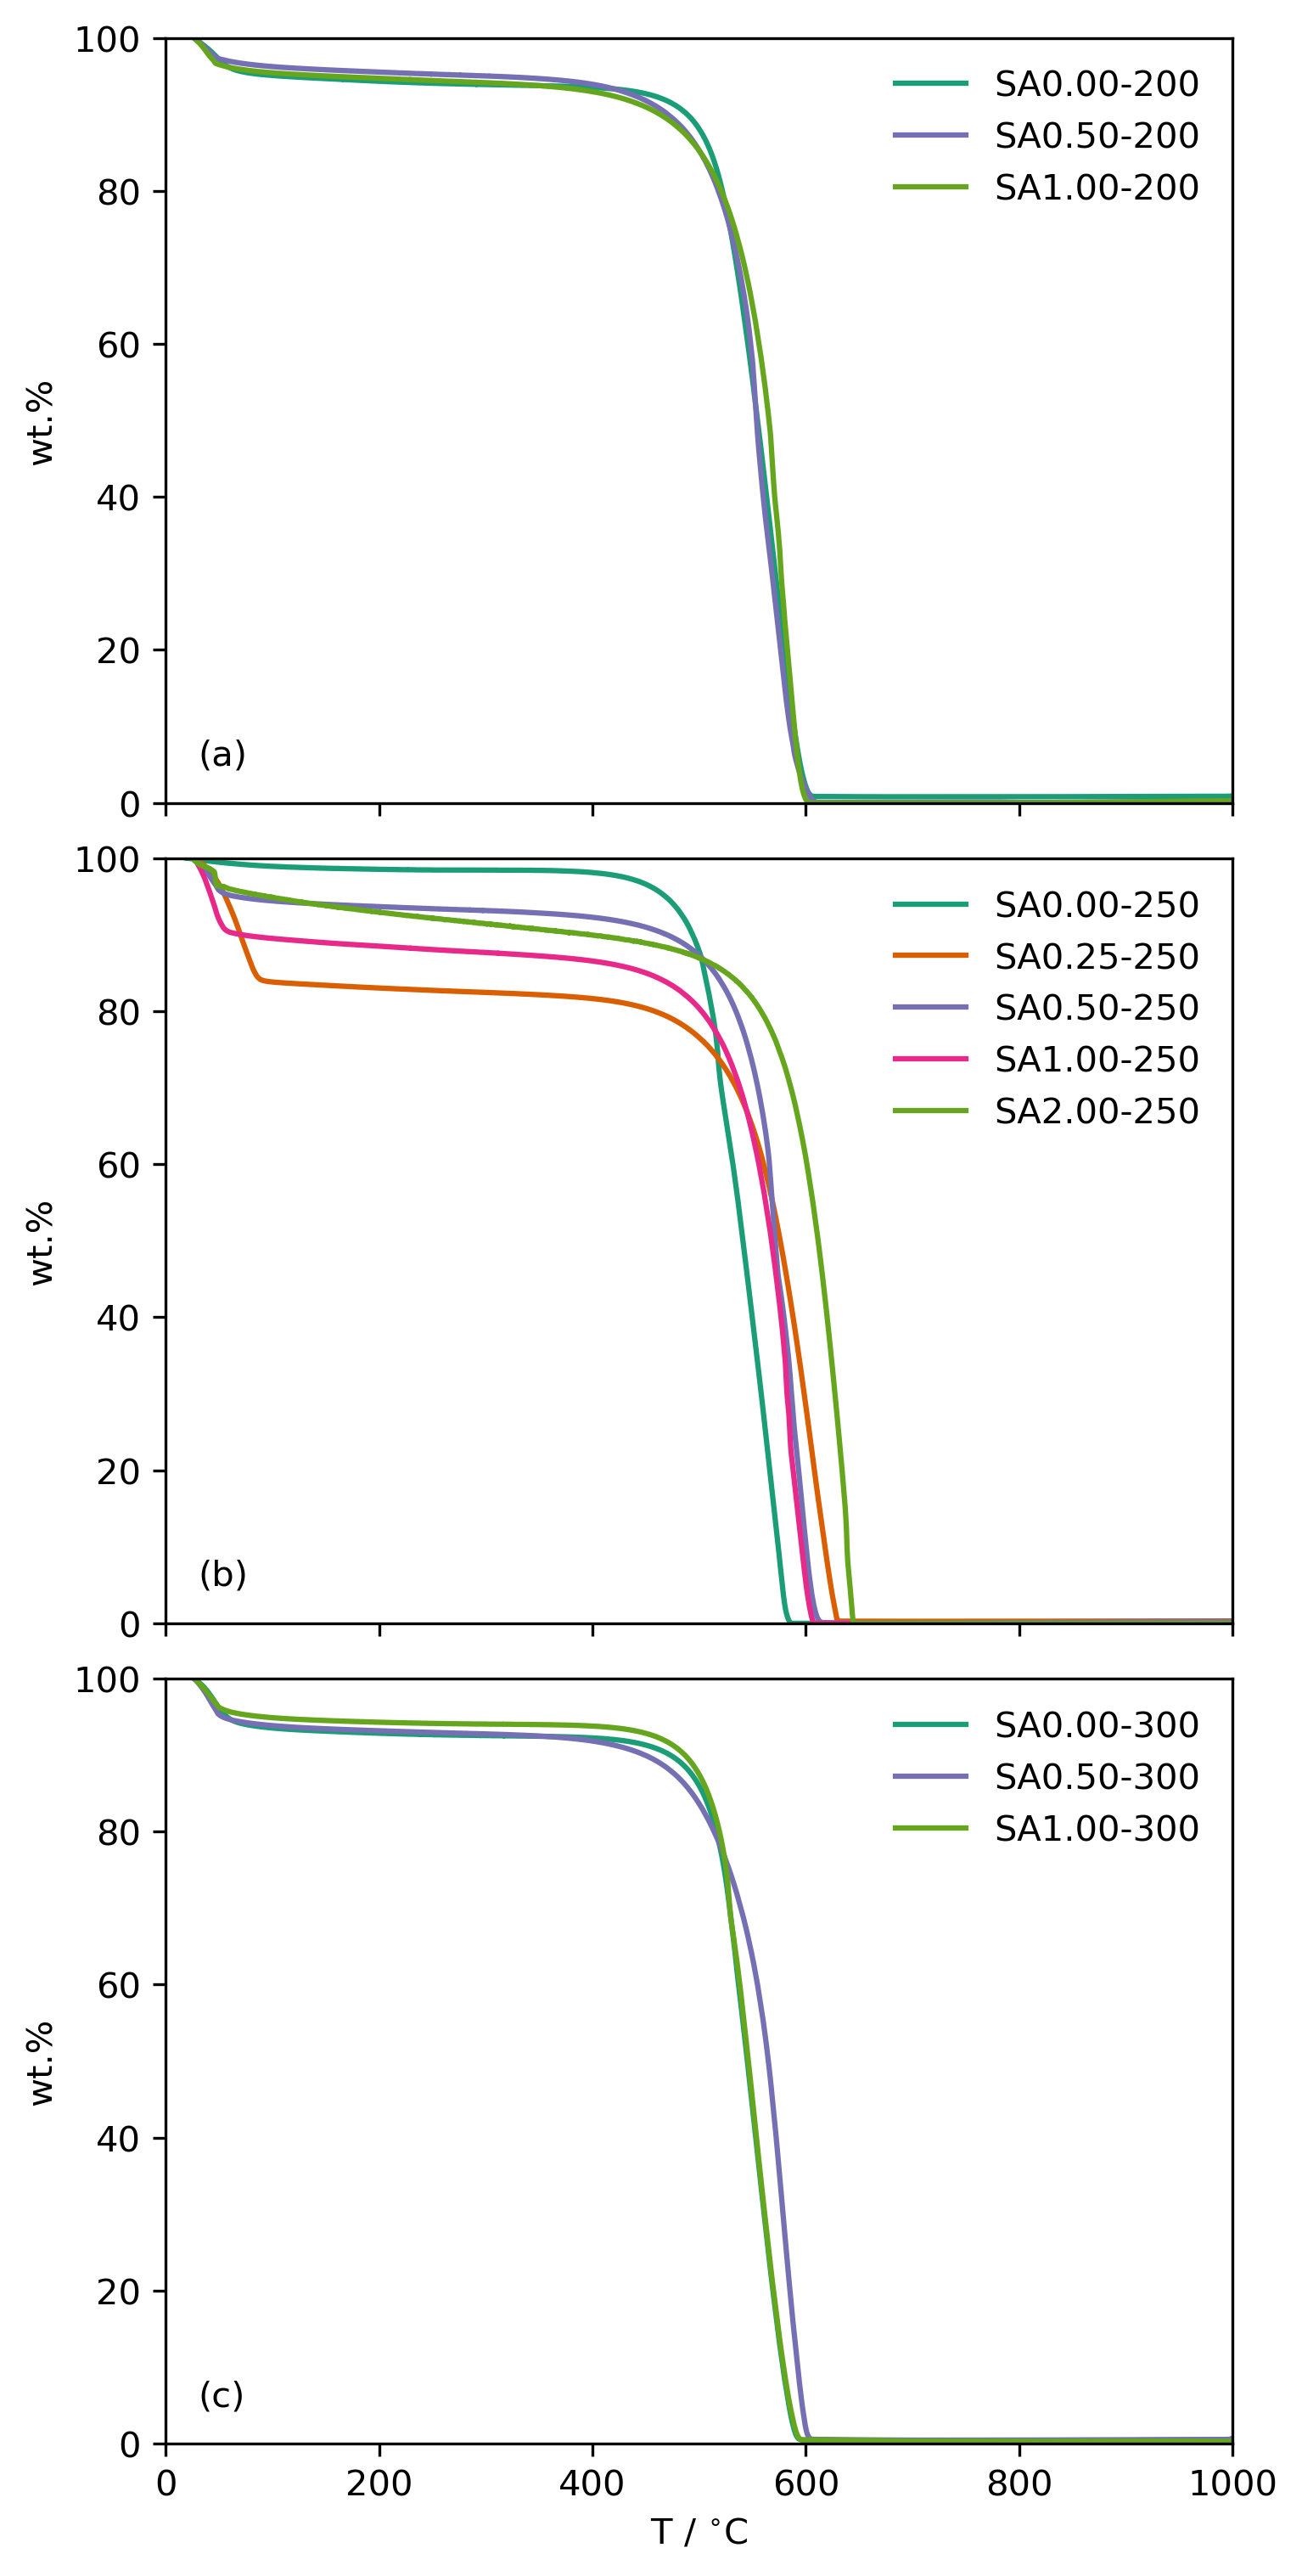
\includegraphics[width=0.8\columnwidth, keepaspectratio]{4-impregnation/figs/SD_tga_adj.png}
    \caption{TGA curves for SD\textit{x.xx-HHH} samples.}
    \label{fig:SD_tga}
\end{figure}

\chapter{Porosimetry}

\newpage
\begin{figure}[p]
    \centering
    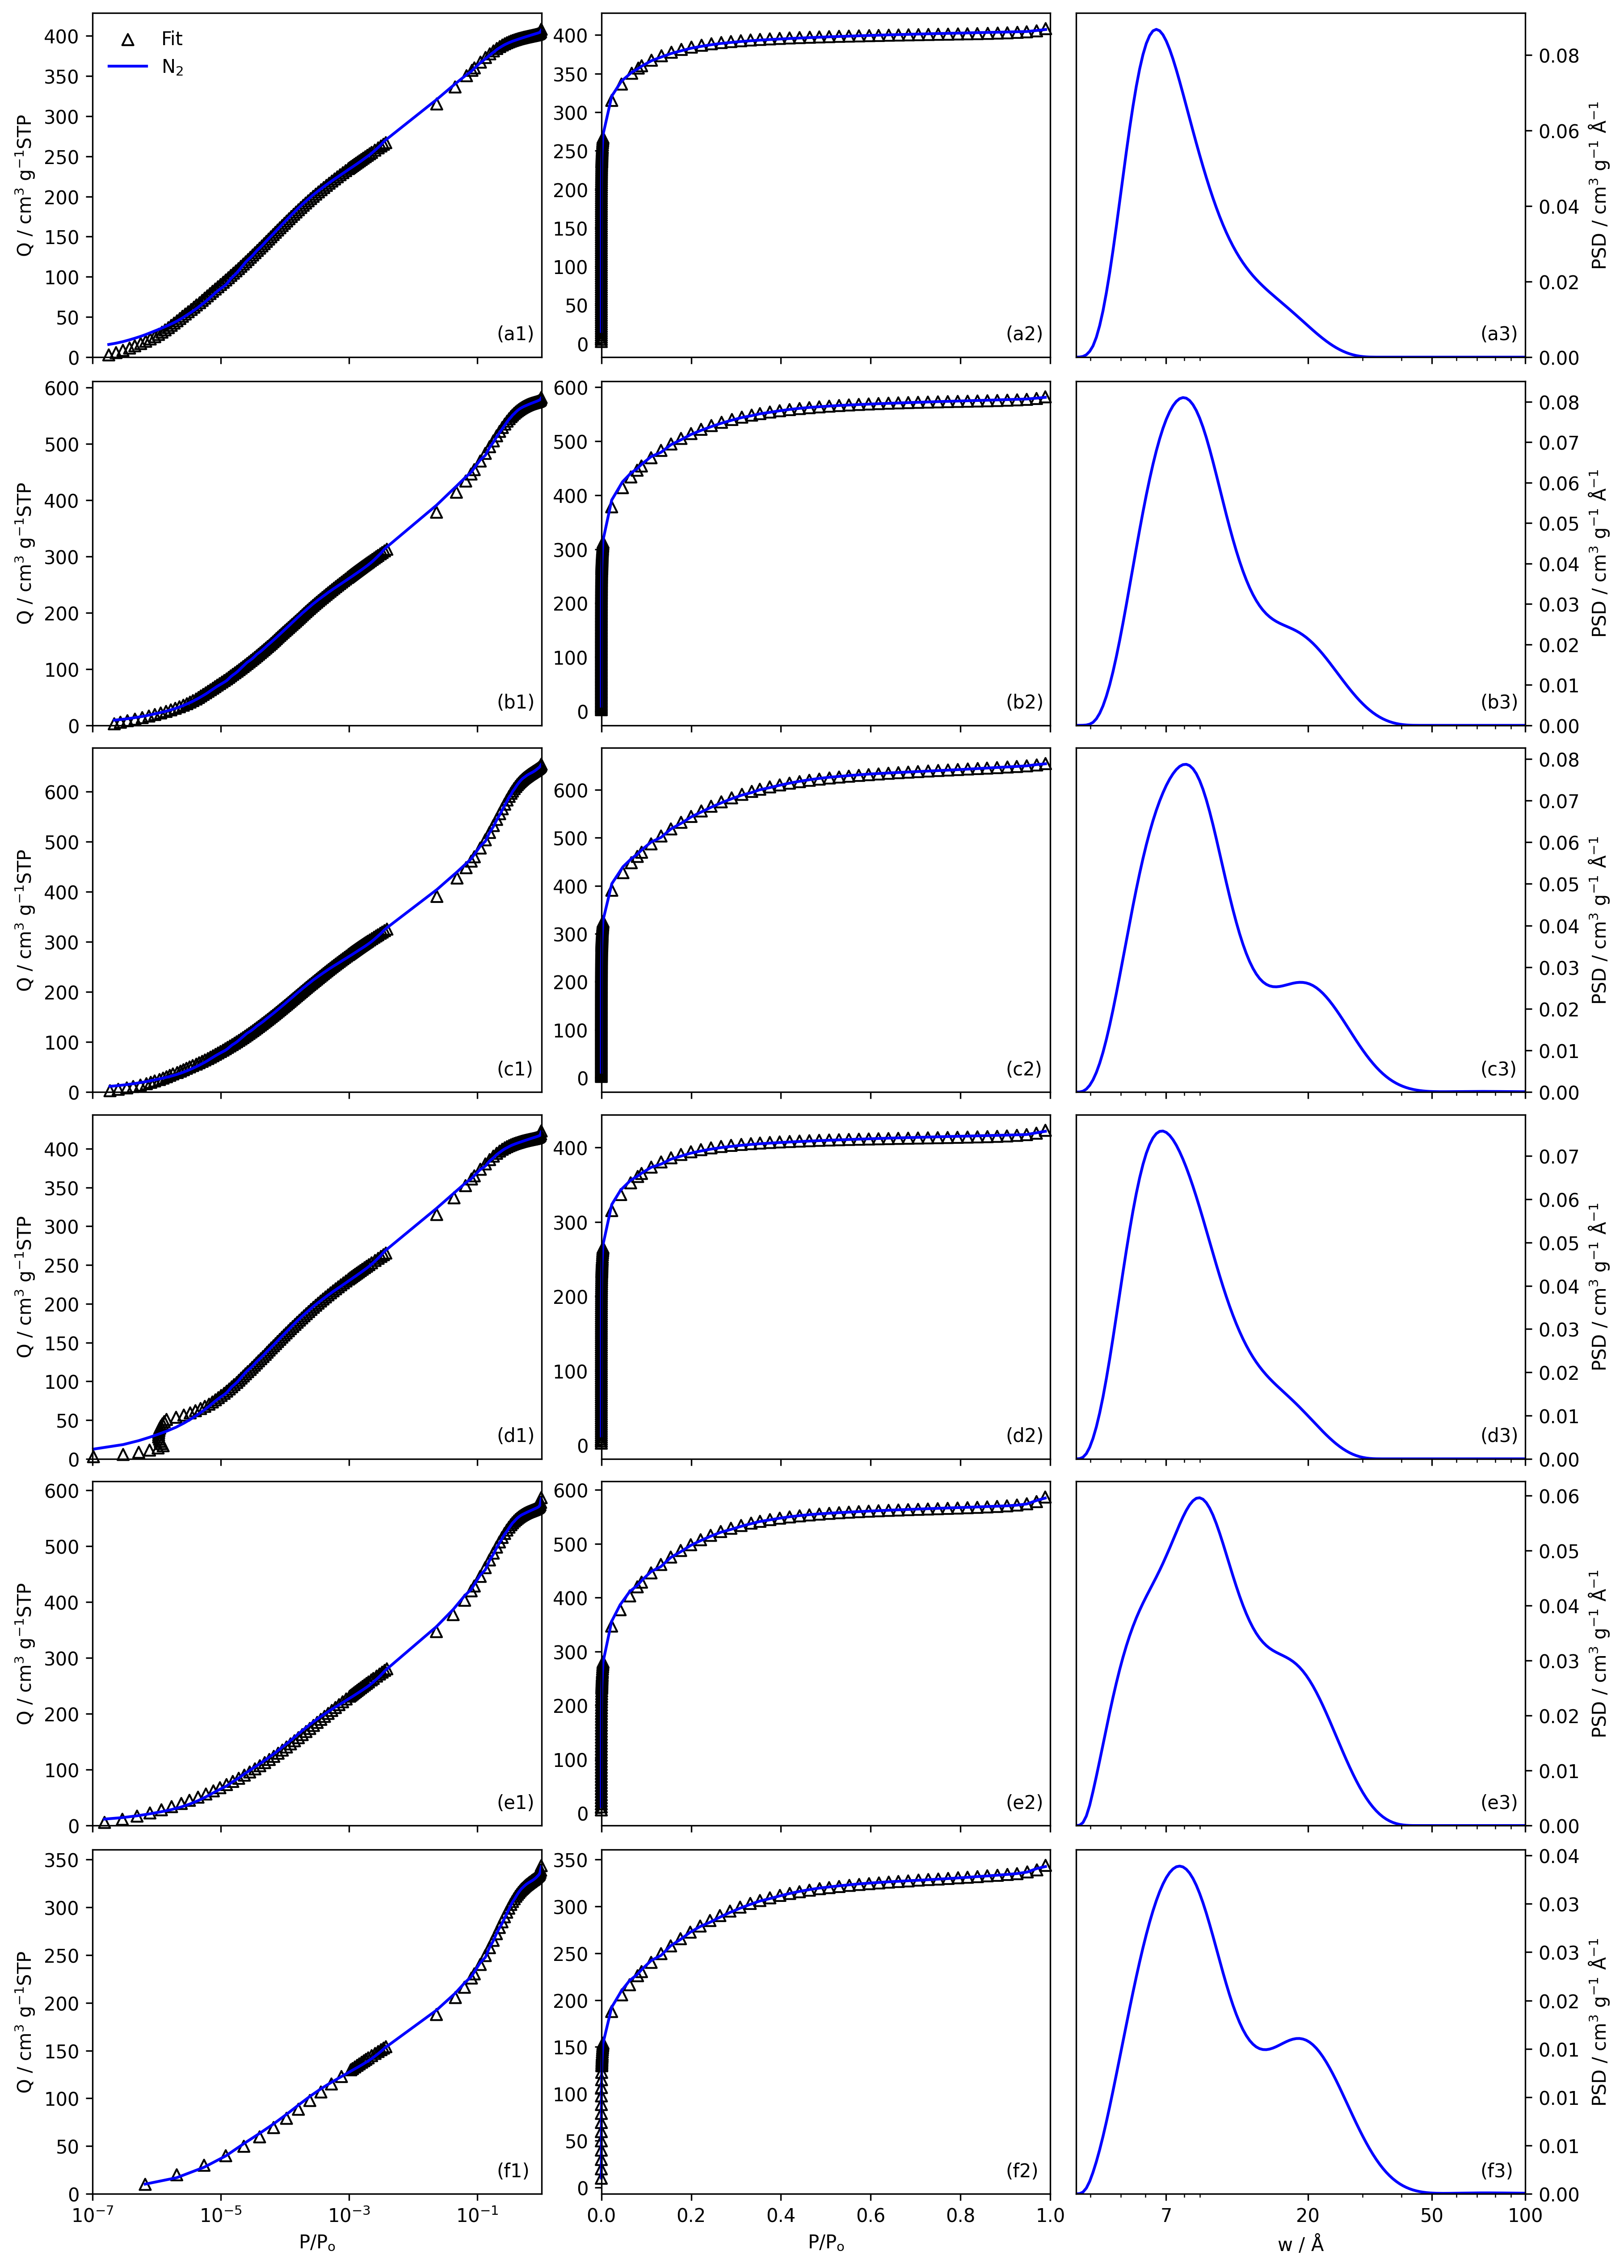
\includegraphics[width=\columnwidth, keepaspectratio]{4-cbs/figs/CB-4TTT_isopsd.png}
    \caption{Fits to \ce{N2} isotherms with logarithmic (a) and linear (b) relative pressure scale, and resultant differential PSDs (c) for samples hC-4600, hC-4700, hC-4800, hD-4600, hD-4700, hD-4800 in order in rows (1-6).}
    \label{fig:4TTT_psdisofull}
\end{figure}

\begin{figure}[p]
    \centering
    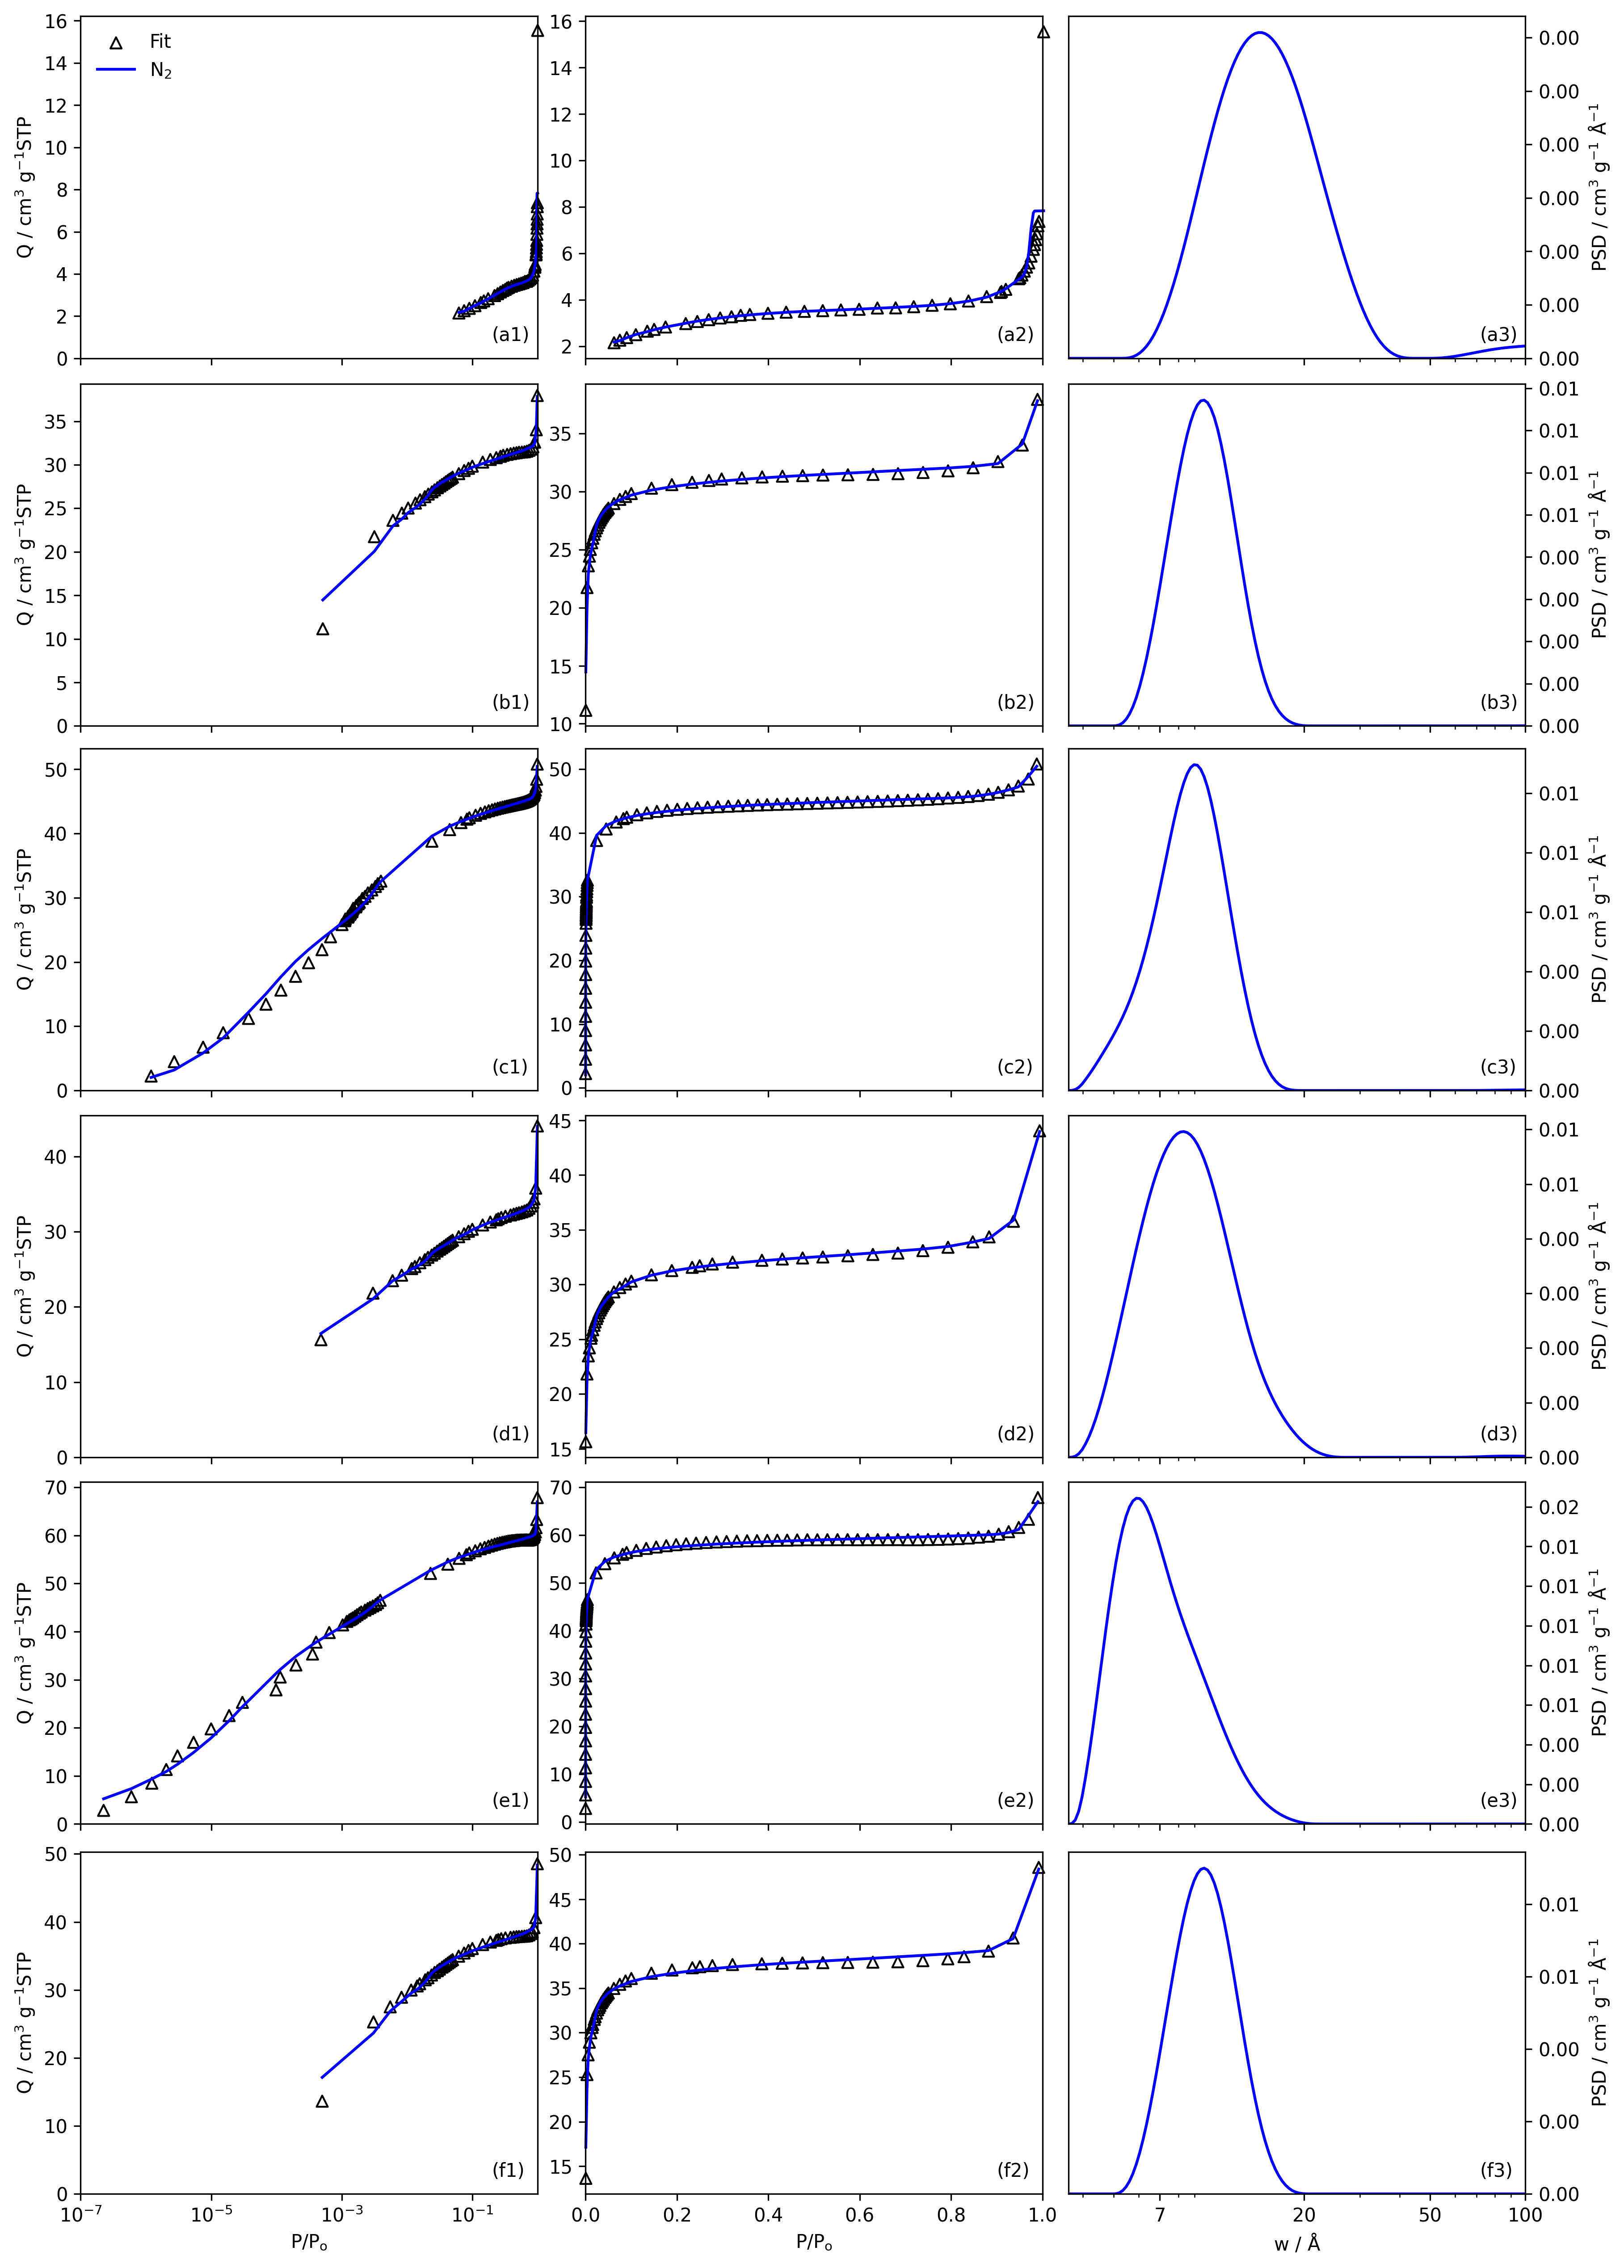
\includegraphics[width=\columnwidth, keepaspectratio]{4-cbs/figs/CB-0TTT_isopsd.png}
    \caption{Fits to \ce{N2} isotherms with logarithmic (a) and linear (b) relative pressure scale, and resultant differential PSDs (c) for samples hD-0600, hD-0700, hD-0800, hD-0600$'$, hD-0700$'$, and hD-0800$'$ in order in rows (1-6).}
    \label{fig:0TTT_psdisofull}
\end{figure}

\begin{figure}[h]
    \centering
    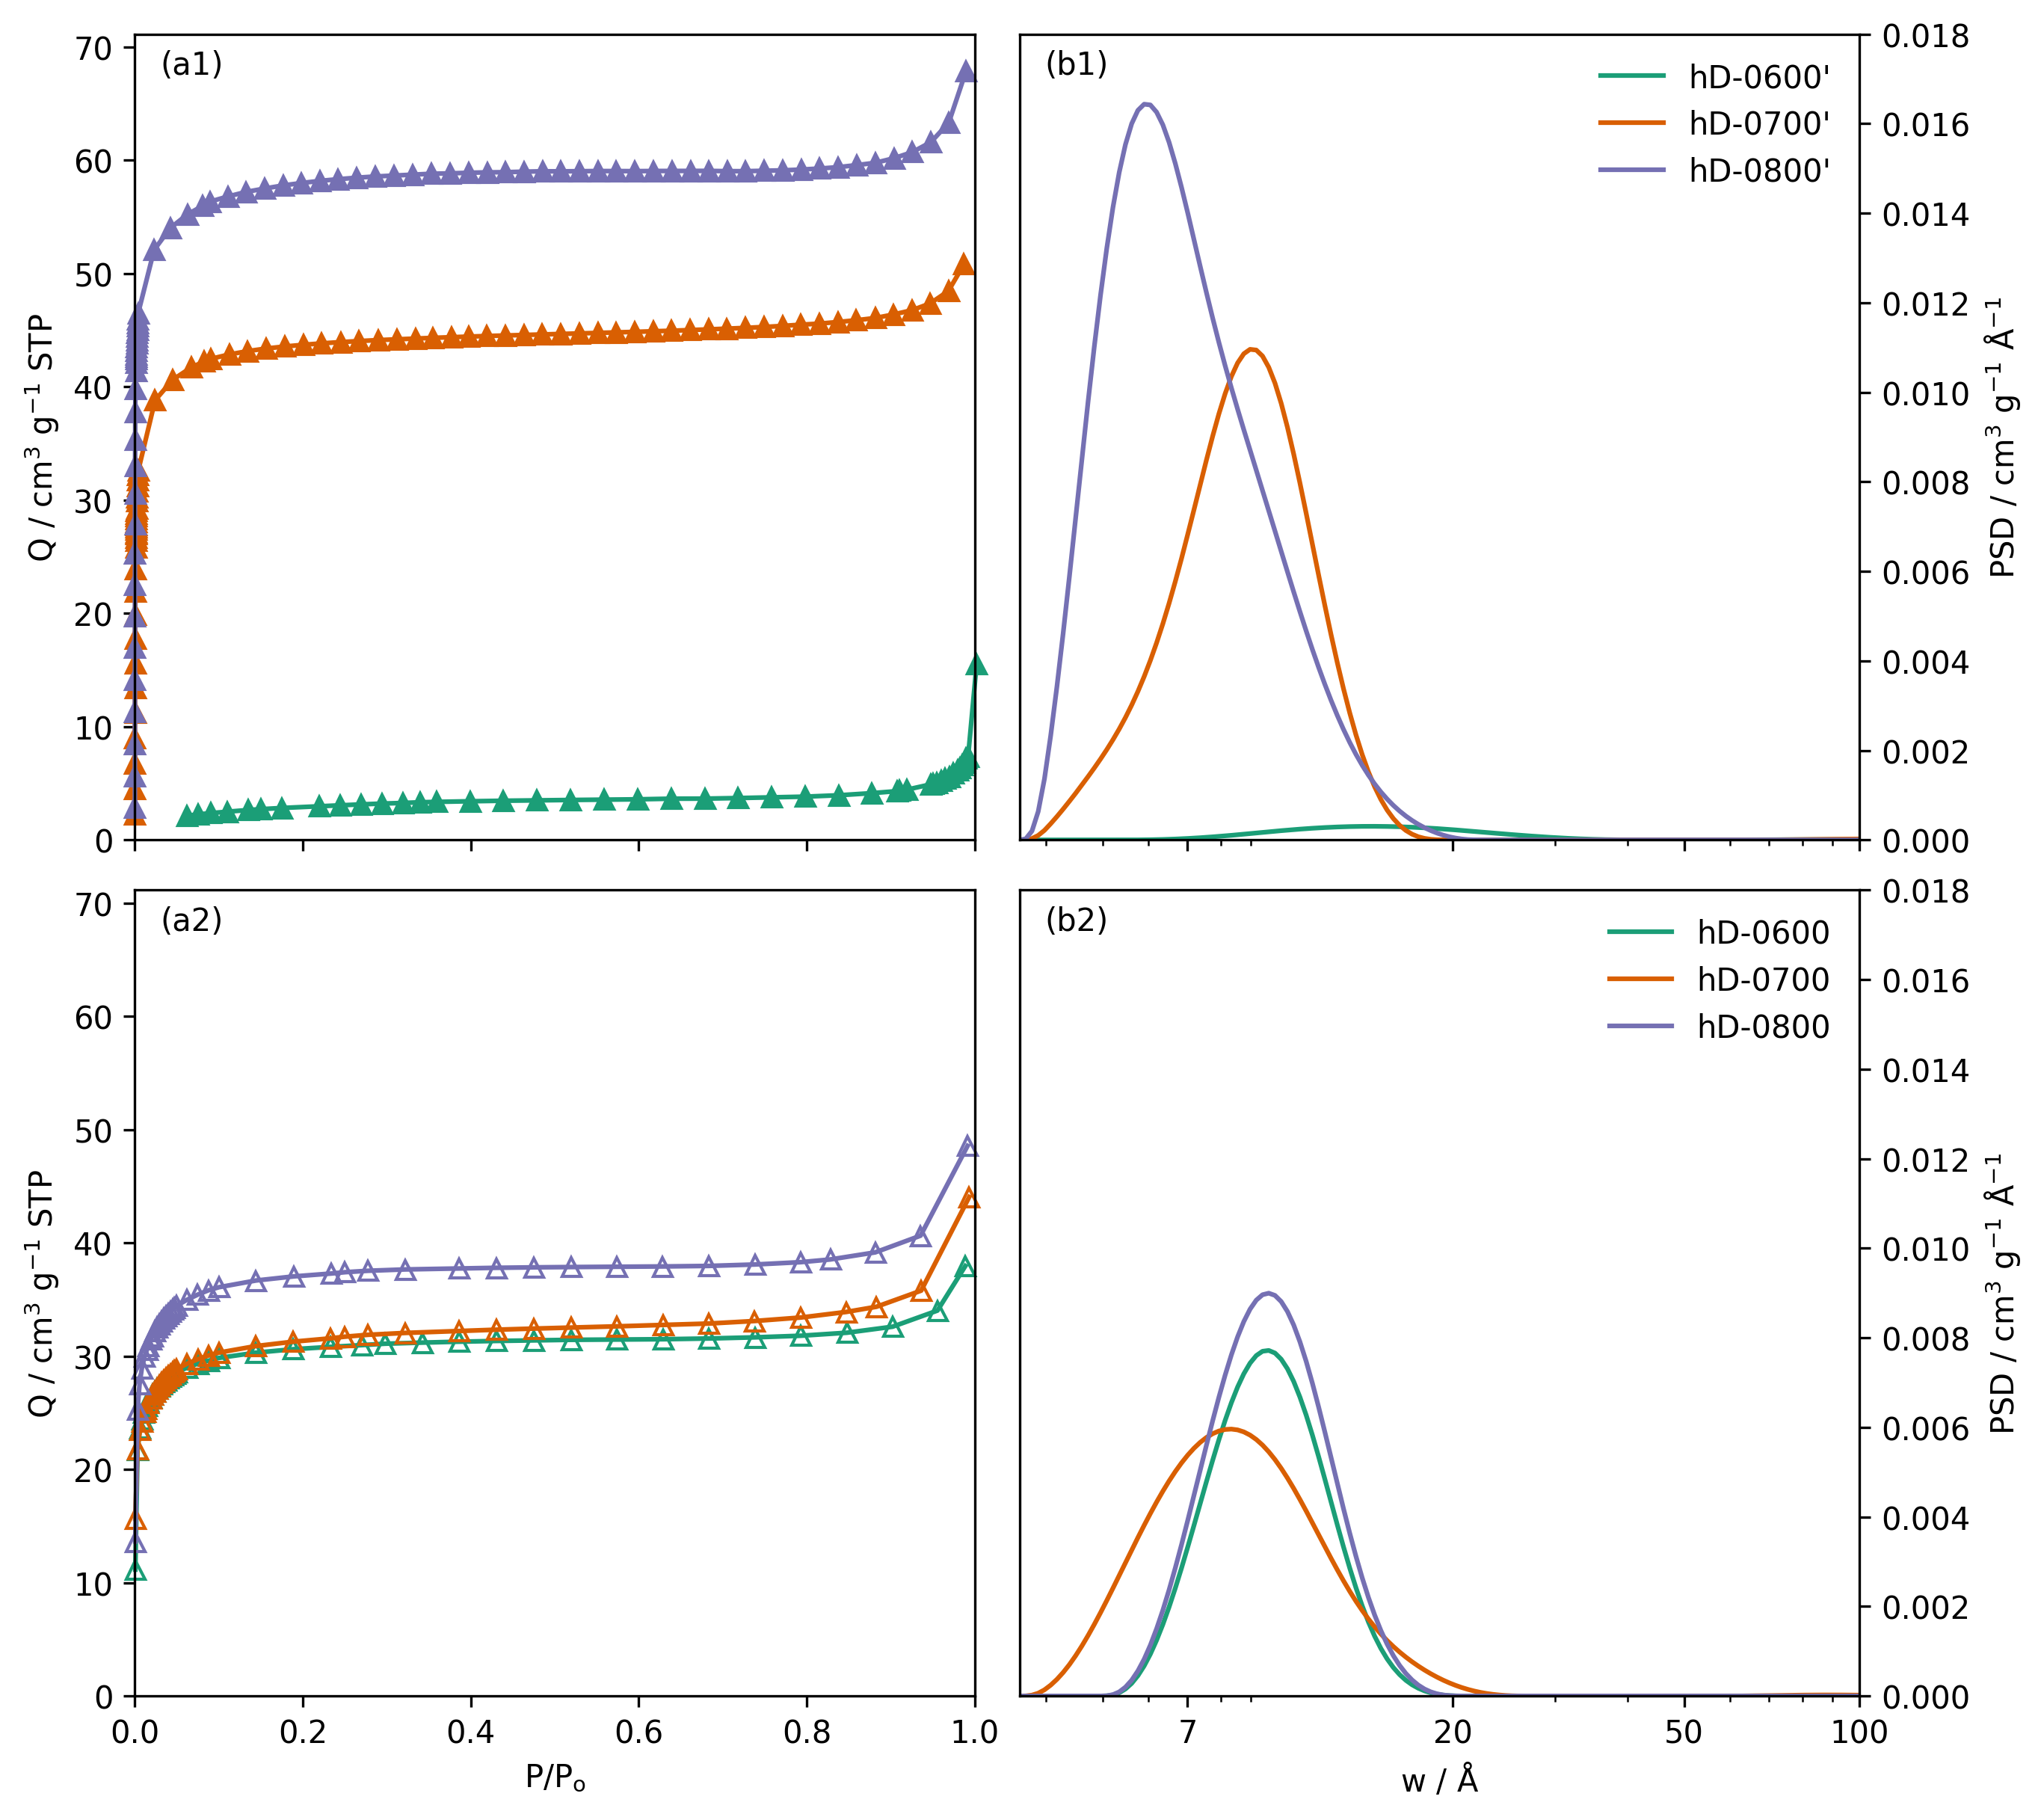
\includegraphics[width=\columnwidth, keepaspectratio]{4-cbs/figs/0TTT_n2_isotherms.png}
    \caption{Isotherms and resultant PSDs for samples hD-0\textit{TTT} and hD-0\textit{TTT}$'$.}
    \label{fig:0TTT_psdiso}
\end{figure}


\begin{figure}[h]
    \centering
    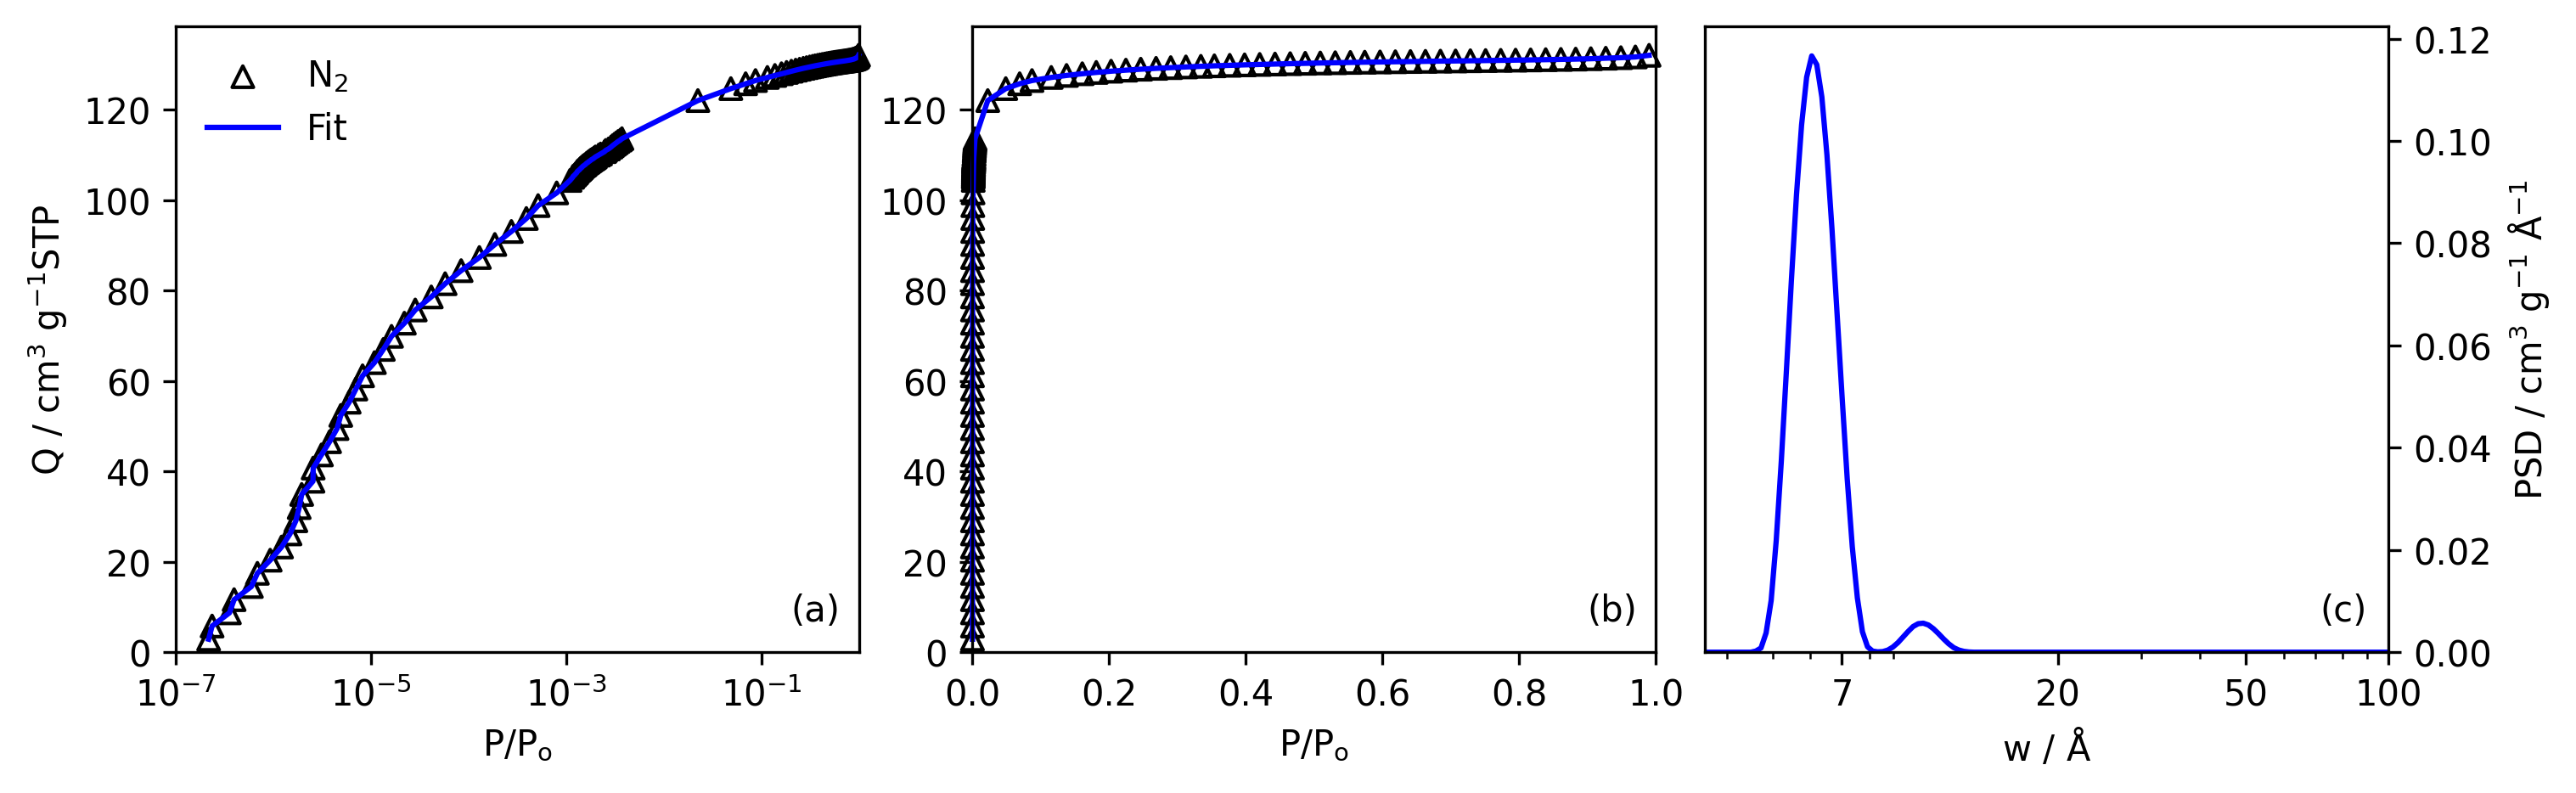
\includegraphics[width=\columnwidth, keepaspectratio]{4-cbs/figs/CA_iso_psd.png}
    \caption{Fits to \ce{N2} isotherms with logarithmic (a) and linear (b) relative pressure scale, and resultant differential PSDs (c) for the cellulose acetate derived sample CA-0800.}
    \label{fig:CA_psdiso}
\end{figure}

\clearpage
\begin{table}[h]
    \centering
    \caption{Porosity of CA-0800}
    \label{tb:CA_porosity}
    \begin{tabularx}{0.9\textwidth}{llllll}
    \toprule
        \multicolumn{2}{l}{$\mathbf{A_{BET}\ /\ m^2\ g^{-1}}$}  & \multicolumn{2}{l}{\textbf{Pore volume} / $\mathbf{cm^3\ g^{-1}}$} & \multicolumn{2}{l}{\textbf{Pore size / \AA}} \\
    \midrule
    522 & (491) & 0.20 & (0.19) & 6 \\
    \bottomrule
    \end{tabularx}
\end{table}

\begin{figure}[p]
    \centering
    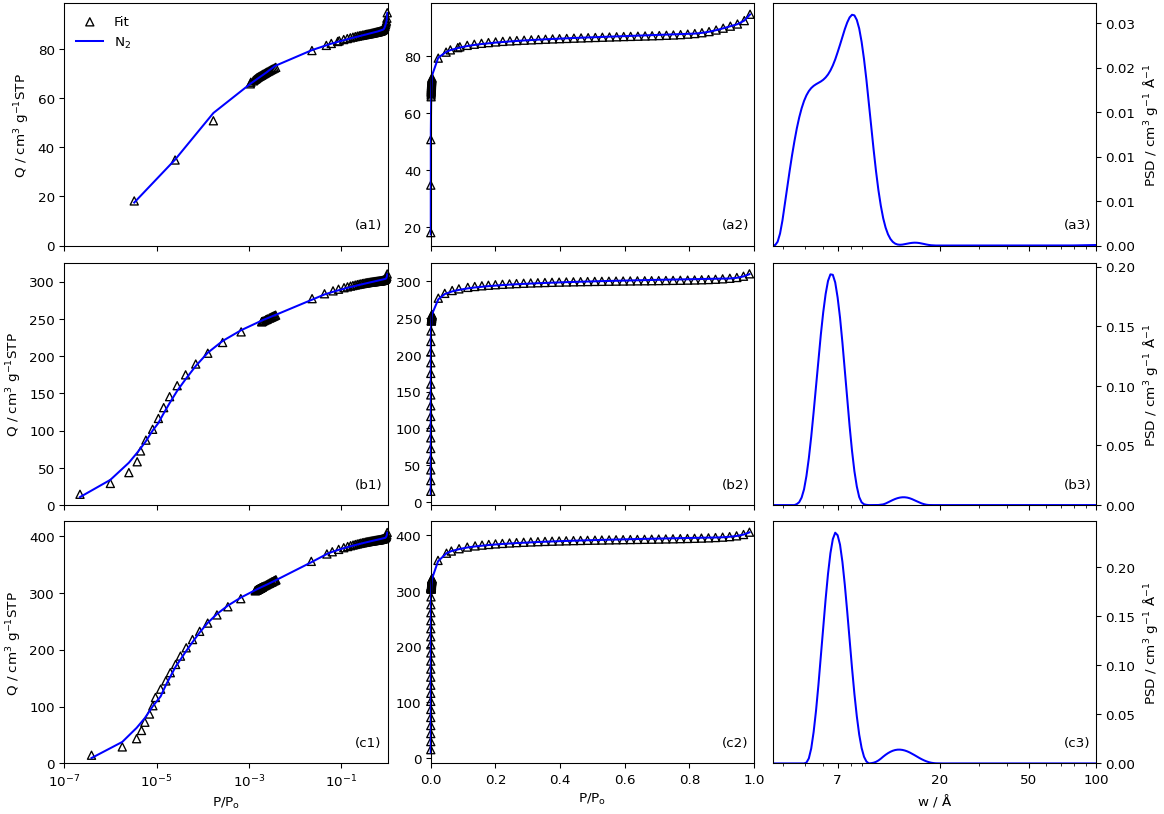
\includegraphics[width=\columnwidth, keepaspectratio]{4-impregnation/figs/SAxxx-200_isopsd.png}
    \caption{Fits to \ce{N2} isotherms with logarithmic (a) and linear (b) relative pressure scale, and resultant differential PSDs (c) for samples SA0.00-200, SA0.50-200, and SA1.00-200 in order in rows (1-3).}
    \label{fig:SAxxx-200_isopsd}
\end{figure}

\begin{figure}[p]
    \centering
    \includegraphics[width=\columnwidth, keepaspectratio]{4-impregnation/figs/SAxxx-250_isopsd.png}
    \caption{Fits to \ce{N2} isotherms with logarithmic (a) and linear (b) relative pressure scale, and resultant differential PSDs (c) for samples SA0.00-250, SA0.25-250, SA0.50-250, SA1.0-250, and SA2.00-250 in order in rows (1-5).}
    \label{fig:SAxxx-250_isopsd}
\end{figure}

\begin{figure}[p]
    \centering
    \includegraphics[width=\columnwidth, keepaspectratio]{4-impregnation/figs/SAxxx-300_isopsd.png}
    \caption{Fits to \ce{N2} isotherms with logarithmic (a) and linear (b) relative pressure scale, and resultant differential PSDs (c) for samples SA0.00-300, SA0.50-300, and SA1.00-300 in order in rows (1-3).}
    \label{fig:SAxxx-300_isopsd}
\end{figure}

\begin{figure}[p]
    \centering
    \includegraphics[width=0.87\columnwidth, keepaspectratio]{4-impregnation/figs/NC_tga.png}
    \caption{Unadjusted TGA curves for NC\textit{x.x-TTT} samples.}
    \label{fig:NC_tga}
\end{figure}

\begin{figure}[p]
    \centering
    \includegraphics[width=\columnwidth, keepaspectratio]{4-impregnation/figs/NCxx-600_isopsd.png}
    \caption{Fits to \ce{N2} isotherms with logarithmic (a) and linear (b) relative pressure scale, and resultant differential PSDs (c) for samples NC0.0-600, NC0.7-600, NC0.9-600, and NC1.2-600 in order in rows (1-4).}
    \label{fig:NCxx-600_psdisofull}
\end{figure}

\begin{figure}[p]
    \centering
    \includegraphics[width=\columnwidth, keepaspectratio]{4-impregnation/figs/NCxx-700_isopsd.png}
    \caption{Fits to \ce{N2} isotherms with logarithmic (a) and linear (b) relative pressure scale, and resultant differential PSDs (c) for samples NC0.0-700, NC0.7-700, NC0.9-700, and NC1.2-700 in order in rows (1-4).}
    \label{fig:NCxx-700_psdisofull}
\end{figure}

\begin{figure}[p]
    \centering
    \includegraphics[width=\columnwidth, keepaspectratio]{4-impregnation/figs/NCxx-800_isopsd.png}
    \caption{Fits to \ce{N2} isotherms with logarithmic (a) and linear (b) relative pressure scale, and resultant differential PSDs (c) for samples NC0.0-800, NC0.7-800, NC0.9-800, and NC1.2-800 in order in rows (1-4).}
    \label{fig:NCxx-800_psdisofull}
\end{figure}

\begin{figure}[p]
    \centering
    \includegraphics[width=\columnwidth, keepaspectratio]{4-impregnation/figs/hyst.png}
    \caption{Demonstration of the permanence of the hysteresis loop for \ce{N2} isotherms on \acrshort{nc} samples (NC0.9-800 in this case) even when isotherm is given longer to equilibrate during the desorption branch. Small discrepancies in the adsorption branch are likely due to errors in measurement of sample mass.}
    \label{fig:hyst}
\end{figure}

\begin{figure}[hptb]
    \centering
    \includegraphics[width=\columnwidth, keepaspectratio]{5-dual_isotherm/figs/SA050-xxx_isopsd.png}
    \caption{Changes in porosity with \gls{htc} temperature for SA0.5-\textit{TTT} carbons. Compared according to dual fit \ce{N2}/\ce{H2} (1) and \ce{O2}/\ce{H2} (2) porosimetry.}
    \label{fig:SA050-xxx_isopsd}
\end{figure}

\begin{figure}[hptb]
    \centering
    \includegraphics[width=\columnwidth, keepaspectratio]{5-dual_isotherm/figs/SA100-xxx_isopsd.png}
    \caption{Changes in porosity with \gls{htc} temperature for SA1.0-\textit{TTT} carbons. Compared according to dual fit \ce{N2}/\ce{H2} (1) and \ce{O2}/\ce{H2} (2) porosimetry.}
    \label{fig:SA100-xxx_isoposd}
\end{figure}

\chapter{Computation}
\newpage

\begin{figure}[h]
\centering
    \begin{verbatim}
        
    Loading DataFrame generated at 15:09 on 22-01-26
    ------------------------------------------------
    
    Project name = 0000_example, Sorptive = co2, T = 298 K
    Models used = ['Langmuir', 'DSLangmuir', 
                    'TSLangmuir', 'GAB', 
                    'Freundlich', 'DR', 'Toth'], 
    Number of isotherms = 4
    Pressure range = 1.0 - 4.0 bar, with increment 1.0
                
    \end{verbatim}
    \captionof{figure}{An example of the report generated after processing experimental uptake isotherms with pyPUC.\\}
    \label{fig:loading_report}
    
    \centering
    \begin{verbatim}
    
    Parameter DataFrame generated at 15:08 on 22-01-26 
    ------------------------------------------------
    
    Project name = 0000_example, Sorptives = n2h2,
    Number of PSDs = 4, calculated for surface area.
    Using pore widths between 4.0 and 7.0 A with a 
    minimum increment of 1.0 A
                
    \end{verbatim}
    \captionof{figure}{An example of the report generated after processing experimental \acrshortpl{psd} with pyPUC.}
    \label{fig:psd_report}
\end{figure}

\end{appendices}





\end{document}